\input{lib/config.tex}
\usepackage{listings}
\usepackage{graphicx}
\usepackage{ragged2e}
\begin{document}

\onecolumn\begin{@twocolumntrue}
    \begin{minipage}{0.3\textwidth}{\def\svgwidth{0.97\columnwidth}\input{fig/Escudo_UD.eps_tex}}
    \end{minipage}
    \vspace{10pt}
    \begin{minipage}{0.677\textwidth}
        \begin{center}
            \vspace{12mm}
        
            \Large{\textbf {{Makefile Taller OpenMP}}
            \vspace{3mm}
            
            \large{\textbf {Samuel Esteban Paredes Benavides, 20201135050, Johann Mauricio Guevara Hernández, 20211107013}}
            \vspace{2mm}
    
            \large{\textit{Sistemas Distribuidos, Programa Académico de Física}}
            \vspace{1mm}
            \large{\textit{Universidad Distrital Francisco José de Caldas}}
            \vspace{1mm}

            \large{\today}
        \end{center}
\vspace{5pt}
\end{minipage}

\centerline{\rule{0.95\textwidth}{0.4pt}}
\end{@twocolumntrue}

\section{Propuesta del Proyecto y Objetivos}

\subsection{Descripción de la Asignatura y el Reto}
El presente trabajo se enmarca dentro de la asignatura \textbf{Sistemas Distribuidos}, bajo la tutoría del docente \textbf{Carlos Andrés Gómez Vasco}. 

\textbf{Objetivo Principal:} 
Aplicar diferentes directivas de la API OpenMP para paralelizar un código secuencial escrito en C++ que resuelve la ecuación de Poisson 2D mediante el método numérico de diferencias finitas. A través de este proceso, se busca analizar exhaustivamente el impacto de cada estrategia de paralelización (y sincronización) en el rendimiento computacional, la escalabilidad y la estructura del programa.

Para lograr este objetivo, el taller plantea una progresión estructurada a través de siete actividades clave:
\begin{enumerate}
    \item Implementación del paralelismo básico en bucles (\texttt{\#pragma omp parallel for}) manejando reducciones para evitar condiciones de carrera.
    \item Aceleración de bucles anidados mediante la directiva \texttt{collapse(2)}.
    \item Ejecución de funciones independientes en paralelo utilizando \texttt{sections}.
    \item Control explícito de las regiones paralelas y evaluación de políticas de planificación (\texttt{schedule(static)} vs \texttt{schedule(dynamic)}).
    \item Control detallado de la sincronización de hilos empleando \texttt{nowait}, \texttt{barrier}, \texttt{single} y \texttt{critical}.
    \item Conteo de iteraciones globales comparando el rendimiento y la seguridad del acceso a memoria compartida entre \texttt{critical} y \texttt{atomic}.
    \item Exploración de paralelismo asíncrono y partición del dominio mediante la directiva orientada a tareas (\texttt{task}).
\end{enumerate}

\subsection{Ejercicios Propuestos: Ecuación de Poisson 2D}
La ecuación de Poisson es una ecuación diferencial parcial elíptica de segundo orden, de gran utilidad en física e ingeniería para describir campos potenciales (eléctricos, gravitatorios, de temperatura, entre otros). En su forma bidimensional, se expresa como:

\begin{equation}
    \nabla^2 u = \frac{\partial^2 u}{\partial x^2} + \frac{\partial^2 u}{\partial y^2} = f(x,y)
\end{equation}

Para evaluar la robustez y exactitud de los métodos numéricos implementados a lo largo del proyecto, se proponen cuatro problemas de contorno de Dirichlet distintos. En cada caso, se conoce la función fuente $f(x,y)$ y la solución analítica exacta $u(x,y)$, la cual se emplea tanto para establecer las condiciones de frontera en los bordes del dominio espacial como para validar el error de la solución numérica aproximada.

A continuación, se presentan las cuatro ecuaciones diferenciales a resolver:

\subsubsection*{Ejercicio 1}
Resolver la ecuación de Poisson en un dominio rectangular con una función fuente exponencial:
\begin{equation}
    \frac{\partial^2 u}{\partial x^2} + \frac{\partial^2 u}{\partial y^2} = (x^2 + y^2)e^{xy}
\end{equation}
\begin{itemize}
    \item \textbf{Dominio Espacial:} $0 < x < 2 \quad \text{y} \quad 0 < y < 1$
    \item \textbf{Solución Analítica (Condición de Frontera):} $u(x,y) = e^{xy}$
\end{itemize}

\subsubsection*{Ejercicio 2 (Ecuación de Laplace)}
Resolver la ecuación de Laplace (un caso especial de la ecuación de Poisson donde la fuente es nula):
\begin{equation}
    \frac{\partial^2 u}{\partial x^2} + \frac{\partial^2 u}{\partial y^2} = 0
\end{equation}
\begin{itemize}
    \item \textbf{Dominio Espacial:} $1 < x < 2 \quad \text{y} \quad 0 < y < 1$
    \item \textbf{Solución Analítica (Condición de Frontera):} $u(x,y) = \ln(x^2 + y^2)$
\end{itemize}

\subsubsection*{Ejercicio 3}
Resolver la ecuación de Poisson con un término fuente constante:
\begin{equation}
    \frac{\partial^2 u}{\partial x^2} + \frac{\partial^2 u}{\partial y^2} = 4
\end{equation}
\begin{itemize}
    \item \textbf{Dominio Espacial:} $1 < x < 2 \quad \text{y} \quad 0 < y < 2$
    \item \textbf{Solución Analítica (Condición de Frontera):} $u(x,y) = (x-y)^2$
\end{itemize}

\subsubsection*{Ejercicio 4}
Resolver la ecuación de Poisson con un término fuente racional:
\begin{equation}
    \frac{\partial^2 u}{\partial x^2} + \frac{\partial^2 u}{\partial y^2} = \frac{x}{y} + \frac{y}{x}
\end{equation}
\begin{itemize}
    \item \textbf{Dominio Espacial:} $1 < x < 2 \quad \text{y} \quad 1 < y < 2$
    \item \textbf{Solución Analítica (Condición de Frontera):} $u(x,y) = xy \ln(xy)$
\end{itemize}

Estos cuatro sistemas matemáticos se centralizaron programáticamente en una cabecera de utilidad (\texttt{utils.h}), garantizando que cualquier experimento de escalabilidad evalúe las cuatro dinámicas físicas de manera consistente.

\section{Implementación de la Ecuación de Poisson 2D con OpenMP}

En esta sección se detalla la solución numérica de la ecuación de Poisson en dos dimensiones utilizando el método de diferencias finitas. Para evaluar las diferentes estrategias de paralelización en memoria compartida, se desarrollaron cinco versiones del código en C++ haciendo uso de las directivas de OpenMP.

\subsection{Códigos Fuente C++}

A continuación se presentan las cinco implementaciones evaluadas. Cada versión inicializa la grilla, aplica la función fuente gaussiana, resuelve el sistema iterativamente hasta alcanzar la convergencia y exporta los resultados a un archivo de datos (\texttt{.dat}).

\subsubsection{Versión 1: Serial (Código Base)}
Esta versión representa la implementación secuencial sin paralelismo, la cual sirve como línea base para calcular la aceleración (\textit{speedup}) de las demás implementaciones.

\begin{lstlisting}[language=C++, caption=Implementación Serial de la Ecuación de Poisson.]
#include <iostream>
#include <vector>
#include <cmath>
#include <algorithm>
#include <fstream>

const double x_0 = 0.0, x_f = 1.0;
const double y_0 = 0.0, y_f = 1.0;
const double e = 8.85e-12; 
const double TOL = 1e-6;

void initialize_grid(int M, int N, std::vector<std::vector<double>>& T, std::vector<std::vector<double>>& source, double& h, double& k) {
    h = (x_f - x_0) / M;
    k = (y_f - y_0) / N;

    T.resize(M + 1, std::vector<double>(N + 1, 0.0));
    source.resize(M + 1, std::vector<double>(N + 1, 0.0));

    for (int j = 0; j <= N; ++j) {
        T[M][j] = 0.0;
        T[0][j] = 0.0;
    }
    for (int i = 0; i <= M; ++i) {
        T[i][0] = 0.0;
        T[i][N] = std::pow(x_0 + i * h, 1.0);
    }
}

void poisson_source(int M, int N, std::vector<std::vector<double>>& source, double h, double k) {
    double mu = 0.5, sigma = 0.1;
    for (int i = 0; i <= M; ++i) {
        for (int j = 0; j <= N; ++j) {
            double x = x_0 + i * h;
            double y = y_0 + j * k;
            source[i][j] = std::exp(-((x - mu)*(x - mu) + (y - mu)*(y - mu)) / (2 * sigma * sigma)) / (std::sqrt(2 * M_PI * sigma));
            if (i == 0 || i == M || j == 0 || j == N) {
                source[i][j] = 0.0;
            }
        }
    }
}

void solve_poisson(std::vector<std::vector<double>>& T, const std::vector<std::vector<double>>& source, int M, int N, double h, double k) {
    double constante = 1.0 / e;
    double delta = 1.0;

    while (delta > TOL) {
        delta = 0.0;
        for (int i = 1; i < M; ++i) {
            for (int j = 1; j < N; ++j) {
                double T_new = (
                    ((T[i + 1][j] + T[i - 1][j]) * k * k) +
                    ((T[i][j + 1] + T[i][j - 1]) * h * h) -
                    (constante * source[i][j] * h * h * k * k)) /
                    (2.0 * (h * h + k * k));

                delta = std::max(delta, std::abs(T_new - T[i][j]));
                T[i][j] = T_new;
            }
        }
    }
}

void export_to_file(const std::vector<std::vector<double>>& T, double h, double k, int M, int N, const std::string& filename) {
    std::ofstream file(filename);
    if (!file.is_open()) {
        std::cerr << "No se pudo abrir el archivo para escritura." << std::endl;
        return;
    }
    for (int i = 0; i <= M; ++i) {
        for (int j = 0; j <= N; ++j) {
            double x = x_0 + i * h;
            double y = y_0 + j * k;
            file << x << "\t" << y << "\t" << T[i][j] << "\n";
        }
    }
    file.close();
}

int main() {
    int M = 50, N = 50;
    double h, k;
    std::vector<std::vector<double>> T, source;

    initialize_grid(M, N, T, source, h, k);
    poisson_source(M, N, source, h, k);
    solve_poisson(T, source, M, N, h, k);

    export_to_file(T, h, k, M, N, "data/solucion_serial.dat");
    std::cout << "[Serial] Simulación completada." << std::endl;
    return 0;
}
\end{lstlisting}

\subsubsection{Versión 2: Parallel For (Collapse)}
\begin{lstlisting}[language=C++, caption=Implementación utilizando \texttt{\#pragma omp parallel for collapse(2)}.]
#include <iostream>
#include <vector>
#include <cmath>
#include <algorithm>
#include <fstream>
#include <omp.h>

const double x_0 = 0.0, x_f = 1.0;
const double y_0 = 0.0, y_f = 1.0;
const double e = 8.85e-12; 
const double TOL = 1e-6;

void initialize_grid(int M, int N, std::vector<std::vector<double>>& T, std::vector<std::vector<double>>& source, double& h, double& k) {
    h = (x_f - x_0) / M;
    k = (y_f - y_0) / N;

    T.resize(M + 1, std::vector<double>(N + 1, 0.0));
    source.resize(M + 1, std::vector<double>(N + 1, 0.0));

    for (int j = 0; j <= N; ++j) {
        T[M][j] = 0.0;
        T[0][j] = 0.0;
    }
    for (int i = 0; i <= M; ++i) {
        T[i][0] = 0.0;
        T[i][N] = std::pow(x_0 + i * h, 1.0);
    }
}

void poisson_source(int M, int N, std::vector<std::vector<double>>& source, double h, double k) {
    double mu = 0.5, sigma = 0.1;
    for (int i = 0; i <= M; ++i) {
        for (int j = 0; j <= N; ++j) {
            double x = x_0 + i * h;
            double y = y_0 + j * k;
            source[i][j] = std::exp(-((x - mu)*(x - mu) + (y - mu)*(y - mu)) / (2 * sigma * sigma)) / (std::sqrt(2 * M_PI * sigma));
            if (i == 0 || i == M || j == 0 || j == N) {
                source[i][j] = 0.0;
            }
        }
    }
}

void solve_poisson(std::vector<std::vector<double>>& T, const std::vector<std::vector<double>>& source, int M, int N, double h, double k) {
    double constante = 1.0 / e;
    double delta = 1.0;

    while (delta > TOL) {
        delta = 0.0;
        
        #pragma omp parallel for collapse(2) reduction(max:delta)
        for (int i = 1; i < M; ++i) {
            for (int j = 1; j < N; ++j) {
                double T_new = (
                    ((T[i + 1][j] + T[i - 1][j]) * k * k) +
                    ((T[i][j + 1] + T[i][j - 1]) * h * h) -
                    (constante * source[i][j] * h * h * k * k)) /
                    (2.0 * (h * h + k * k));

                delta = std::max(delta, std::abs(T_new - T[i][j]));
                T[i][j] = T_new;
            }
        }
    }
}

void export_to_file(const std::vector<std::vector<double>>& T, double h, double k, int M, int N, const std::string& filename) {
    std::ofstream file(filename);
    if (!file.is_open()) {
        std::cerr << "No se pudo abrir el archivo para escritura." << std::endl;
        return;
    }
    for (int i = 0; i <= M; ++i) {
        for (int j = 0; j <= N; ++j) {
            double x = x_0 + i * h;
            double y = y_0 + j * k;
            file << x << "\t" << y << "\t" << T[i][j] << "\n";
        }
    }
    file.close();
}

int main() {
    int M = 50, N = 50;
    double h, k;
    std::vector<std::vector<double>> T, source;

    initialize_grid(M, N, T, source, h, k);
    poisson_source(M, N, source, h, k);
    solve_poisson(T, source, M, N, h, k);

    export_to_file(T, h, k, M, N, "data/solucion_parallel_for.dat");
    std::cout << "[Parallel For] Simulación completada." << std::endl;
    return 0;
}
\end{lstlisting}

\subsubsection{Versión 3: Región Crítica (Critical)}
\begin{lstlisting}[language=C++, caption=Implementación sincronizada con \texttt{\#pragma omp critical}.]
#include <iostream>
#include <vector>
#include <cmath>
#include <algorithm>
#include <fstream>
#include <omp.h>

const double x_0 = 0.0, x_f = 1.0;
const double y_0 = 0.0, y_f = 1.0;
const double e = 8.85e-12; 
const double TOL = 1e-6;

void initialize_grid(int M, int N, std::vector<std::vector<double>>& T, std::vector<std::vector<double>>& source, double& h, double& k) {
    h = (x_f - x_0) / M;
    k = (y_f - y_0) / N;

    T.resize(M + 1, std::vector<double>(N + 1, 0.0));
    source.resize(M + 1, std::vector<double>(N + 1, 0.0));

    for (int j = 0; j <= N; ++j) {
        T[M][j] = 0.0;
        T[0][j] = 0.0;
    }
    for (int i = 0; i <= M; ++i) {
        T[i][0] = 0.0;
        T[i][N] = std::pow(x_0 + i * h, 1.0);
    }
}

void poisson_source(int M, int N, std::vector<std::vector<double>>& source, double h, double k) {
    double mu = 0.5, sigma = 0.1;
    for (int i = 0; i <= M; ++i) {
        for (int j = 0; j <= N; ++j) {
            double x = x_0 + i * h;
            double y = y_0 + j * k;
            source[i][j] = std::exp(-((x - mu)*(x - mu) + (y - mu)*(y - mu)) / (2 * sigma * sigma)) / (std::sqrt(2 * M_PI * sigma));
            if (i == 0 || i == M || j == 0 || j == N) {
                source[i][j] = 0.0;
            }
        }
    }
}

void solve_poisson(std::vector<std::vector<double>>& T, const std::vector<std::vector<double>>& source, int M, int N, double h, double k) {
    double constante = 1.0 / e;
    double delta = 1.0;
    int iterations = 0;

    while (delta > TOL) {
        delta = 0.0;
        
        #pragma omp parallel for collapse(2) reduction(max:delta)
        for (int i = 1; i < M; ++i) {
            for (int j = 1; j < N; ++j) {
                double T_new = (
                    ((T[i + 1][j] + T[i - 1][j]) * k * k) +
                    ((T[i][j + 1] + T[i][j - 1]) * h * h) -
                    (constante * source[i][j] * h * h * k * k)) /
                    (2.0 * (h * h + k * k));

                delta = std::max(delta, std::abs(T_new - T[i][j]));
                T[i][j] = T_new;
            }
        }
        
        #pragma omp critical
        {
            iterations++;
        }
    }
    std::cout << "-> Iteraciones completadas (Critical): " << iterations << std::endl;
}

void export_to_file(const std::vector<std::vector<double>>& T, double h, double k, int M, int N, const std::string& filename) {
    std::ofstream file(filename);
    if (!file.is_open()) {
        std::cerr << "No se pudo abrir el archivo para escritura." << std::endl;
        return;
    }
    for (int i = 0; i <= M; ++i) {
        for (int j = 0; j <= N; ++j) {
            double x = x_0 + i * h;
            double y = y_0 + j * k;
            file << x << "\t" << y << "\t" << T[i][j] << "\n";
        }
    }
    file.close();
}

int main() {
    int M = 50, N = 50;
    double h, k;
    std::vector<std::vector<double>> T, source;

    initialize_grid(M, N, T, source, h, k);
    poisson_source(M, N, source, h, k);
    solve_poisson(T, source, M, N, h, k);

    export_to_file(T, h, k, M, N, "data/solucion_critical.dat");
    std::cout << "[Critical] Simulación completada." << std::endl;
    return 0;
}
\end{lstlisting}

\subsubsection{Versión 4: Operaciones Atómicas (Atomic)}
\begin{lstlisting}[language=C++, caption=Implementación sincronizada mediante \texttt{\#pragma omp atomic}.]
#include <iostream>
#include <vector>
#include <cmath>
#include <algorithm>
#include <fstream>
#include <omp.h>

const double x_0 = 0.0, x_f = 1.0;
const double y_0 = 0.0, y_f = 1.0;
const double e = 8.85e-12; 
const double TOL = 1e-6;

void initialize_grid(int M, int N, std::vector<std::vector<double>>& T, std::vector<std::vector<double>>& source, double& h, double& k) {
    h = (x_f - x_0) / M;
    k = (y_f - y_0) / N;

    T.resize(M + 1, std::vector<double>(N + 1, 0.0));
    source.resize(M + 1, std::vector<double>(N + 1, 0.0));

    for (int j = 0; j <= N; ++j) {
        T[M][j] = 0.0;
        T[0][j] = 0.0;
    }
    for (int i = 0; i <= M; ++i) {
        T[i][0] = 0.0;
        T[i][N] = std::pow(x_0 + i * h, 1.0);
    }
}

void poisson_source(int M, int N, std::vector<std::vector<double>>& source, double h, double k) {
    double mu = 0.5, sigma = 0.1;
    for (int i = 0; i <= M; ++i) {
        for (int j = 0; j <= N; ++j) {
            double x = x_0 + i * h;
            double y = y_0 + j * k;
            source[i][j] = std::exp(-((x - mu)*(x - mu) + (y - mu)*(y - mu)) / (2 * sigma * sigma)) / (std::sqrt(2 * M_PI * sigma));
            if (i == 0 || i == M || j == 0 || j == N) {
                source[i][j] = 0.0;
            }
        }
    }
}

void solve_poisson(std::vector<std::vector<double>>& T, const std::vector<std::vector<double>>& source, int M, int N, double h, double k) {
    double constante = 1.0 / e;
    double delta = 1.0;
    int iterations = 0;

    while (delta > TOL) {
        delta = 0.0;
        
        #pragma omp parallel for collapse(2) reduction(max:delta)
        for (int i = 1; i < M; ++i) {
            for (int j = 1; j < N; ++j) {
                double T_new = (
                    ((T[i + 1][j] + T[i - 1][j]) * k * k) +
                    ((T[i][j + 1] + T[i][j - 1]) * h * h) -
                    (constante * source[i][j] * h * h * k * k)) /
                    (2.0 * (h * h + k * k));

                delta = std::max(delta, std::abs(T_new - T[i][j]));
                T[i][j] = T_new;
            }
        }
        
        #pragma omp atomic
        iterations++;
    }
    std::cout << "-> Iteraciones completadas (Atomic): " << iterations << std::endl;
}

void export_to_file(const std::vector<std::vector<double>>& T, double h, double k, int M, int N, const std::string& filename) {
    std::ofstream file(filename);
    if (!file.is_open()) {
        std::cerr << "No se pudo abrir el archivo para escritura." << std::endl;
        return;
    }
    for (int i = 0; i <= M; ++i) {
        for (int j = 0; j <= N; ++j) {
            double x = x_0 + i * h;
            double y = y_0 + j * k;
            file << x << "\t" << y << "\t" << T[i][j] << "\n";
        }
    }
    file.close();
}

int main() {
    int M = 50, N = 50;
    double h, k;
    std::vector<std::vector<double>> T, source;

    initialize_grid(M, N, T, source, h, k);
    poisson_source(M, N, source, h, k);
    solve_poisson(T, source, M, N, h, k);

    export_to_file(T, h, k, M, N, "data/solucion_atomic.dat");
    std::cout << "[Atomic] Simulación completada." << std::endl;
    return 0;
}
\end{lstlisting}

\subsubsection{Versión 5: Tareas por Bloques (Task)}
\begin{lstlisting}[language=C++, caption=Implementación orientada a tareas empleando \texttt{\#pragma omp task}.]
#include <iostream>
#include <vector>
#include <cmath>
#include <algorithm>
#include <fstream>
#include <omp.h>

const double x_0 = 0.0, x_f = 1.0;
const double y_0 = 0.0, y_f = 1.0;
const double e = 8.85e-12; 
const double TOL = 1e-6;

void initialize_grid(int M, int N, std::vector<std::vector<double>>& T, std::vector<std::vector<double>>& source, double& h, double& k) {
    h = (x_f - x_0) / M;
    k = (y_f - y_0) / N;

    T.resize(M + 1, std::vector<double>(N + 1, 0.0));
    source.resize(M + 1, std::vector<double>(N + 1, 0.0));

    for (int j = 0; j <= N; ++j) {
        T[M][j] = 0.0;
        T[0][j] = 0.0;
    }
    for (int i = 0; i <= M; ++i) {
        T[i][0] = 0.0;
        T[i][N] = std::pow(x_0 + i * h, 1.0);
    }
}

void poisson_source(int M, int N, std::vector<std::vector<double>>& source, double h, double k) {
    double mu = 0.5, sigma = 0.1;
    for (int i = 0; i <= M; ++i) {
        for (int j = 0; j <= N; ++j) {
            double x = x_0 + i * h;
            double y = y_0 + j * k;
            source[i][j] = std::exp(-((x - mu)*(x - mu) + (y - mu)*(y - mu)) / (2 * sigma * sigma)) / (std::sqrt(2 * M_PI * sigma));
            if (i == 0 || i == M || j == 0 || j == N) {
                source[i][j] = 0.0;
            }
        }
    }
}

void solve_poisson(std::vector<std::vector<double>>& T, const std::vector<std::vector<double>>& source, int M, int N, double h, double k) {
    double constante = 1.0 / e;
    double delta = 1.0;
    int block_size = 10;

    while (delta > TOL) {
        double max_delta = 0.0;
        
        #pragma omp parallel shared(max_delta)
        {
            #pragma omp single
            {
                for (int bi = 1; bi < M; bi += block_size) {
                    for (int bj = 1; bj < N; bj += block_size) {
                        
                        #pragma omp task shared(max_delta)
                        {
                            double local_delta = 0.0;
                            for (int i = bi; i < std::min(bi + block_size, M); ++i) {
                                for (int j = bj; j < std::min(bj + block_size, N); ++j) {
                                    double T_new = (
                                        ((T[i + 1][j] + T[i - 1][j]) * k * k) +
                                        ((T[i][j + 1] + T[i][j - 1]) * h * h) -
                                        (constante * source[i][j] * h * h * k * k)) /
                                        (2.0 * (h * h + k * k));

                                    local_delta = std::max(local_delta, std::abs(T_new - T[i][j]));
                                    T[i][j] = T_new;
                                }
                            }
                            #pragma omp critical
                            {
                                max_delta = std::max(max_delta, local_delta);
                            }
                        }
                    }
                }
                #pragma omp taskwait
            }
        }
        delta = max_delta;
    }
}

void export_to_file(const std::vector<std::vector<double>>& T, double h, double k, int M, int N, const std::string& filename) {
    std::ofstream file(filename);
    if (!file.is_open()) {
        std::cerr << "No se pudo abrir el archivo para escritura." << std::endl;
        return;
    }
    for (int i = 0; i <= M; ++i) {
        for (int j = 0; j <= N; ++j) {
            double x = x_0 + i * h;
            double y = y_0 + j * k;
            file << x << "\t" << y << "\t" << T[i][j] << "\n";
        }
    }
    file.close();
}

int main() {
    int M = 50, N = 50;
    double h, k;
    std::vector<std::vector<double>> T, source;

    initialize_grid(M, N, T, source, h, k);
    poisson_source(M, N, source, h, k);
    solve_poisson(T, source, M, N, h, k);

    export_to_file(T, h, k, M, N, "data/solucion_task.dat");
    std::cout << "[Task] Simulación completada." << std::endl;
    return 0;
}
\end{lstlisting}

\subsection{Automatización y Medición de Tiempos}

La orquestación de la compilación y ejecución de las distintas versiones se efectuó combinando un \texttt{Makefile} para la gestión de dependencias y un script en Bash para la medición de tiempos.

\begin{lstlisting}[language=bash, caption=Script \texttt{benchmark.sh} para el registro de tiempos de ejecución.]
#!/bin/bash

LOG_FILE="Tiempos_Ejecucion_Poisson.txt"

# Formato limpio para el archivo de texto
echo "Reporte de Tiempos de Ejecución - Taller OpenMP Poisson 2D" > $LOG_FILE
echo "==========================================================" >> $LOG_FILE

# Configurar el formato del comando 'time' de Bash (solo segundos)
TIMEFORMAT="%R segundos"

echo "Iniciando benchmark de tiempos..."

# 1. Ejecutar Secuencial
echo "-> Ejecutando versión Secuencial..."
echo -n "Secuencial          : " >> $LOG_FILE
{ time ./bin/poisson_serial ; } 2>> $LOG_FILE

# 2. Ejecutar Parallel For (Collapse)
echo "-> Ejecutando versión Parallel For (collapse)..."
echo -n "Parallel For        : " >> $LOG_FILE
{ time ./bin/poisson_parallel_for ; } 2>> $LOG_FILE

# 3. Ejecutar Critical
echo "-> Ejecutando versión Critical..."
echo -n "Critical            : " >> $LOG_FILE
{ time ./bin/poisson_critical ; } 2>> $LOG_FILE

# 4. Ejecutar Atomic
echo "-> Ejecutando versión Atomic..."
echo -n "Atomic              : " >> $LOG_FILE
{ time ./bin/poisson_atomic ; } 2>> $LOG_FILE

# 5. Ejecutar Task
echo "-> Ejecutando versión Task..."
echo -n "Task                : " >> $LOG_FILE
{ time ./bin/poisson_task ; } 2>> $LOG_FILE

echo "" >> $LOG_FILE
echo "Ejecución finalizada." >> $LOG_FILE

echo "Benchmark completado. Los resultados se han guardado en $LOG_FILE"
\end{lstlisting}

\begin{lstlisting}[language=make, caption=Archivo \texttt{Makefile} para la automatización del proyecto.]
# ---------------------------------------------------------------------------
# Configuración del compilador y directorios
# ---------------------------------------------------------------------------
CXX      := g++
# Es vital mantener -fopenmp para que el paralelismo funcione
CXXFLAGS := -std=c++17 -O3 -Wall -Wextra -fopenmp -Iinclude

BIN_DIR  := bin
SRC_DIR  := src
DATA_DIR := data
IMAG_DIR := imag
DOC_DIR  := documents

# Encuentra todos los .cpp y genera los nombres de los ejecutables
SRCS := $(wildcard $(SRC_DIR)/*.cpp)
EXES := $(patsubst $(SRC_DIR)/%.cpp, $(BIN_DIR)/%, $(SRCS))

MKDIR_P  := mkdir -p

.PHONY: all run view clean directories docs

all: directories $(EXES)

directories:
    $(MKDIR_P) $(BIN_DIR) $(DATA_DIR) $(IMAG_DIR) $(DOC_DIR)

# Regla de compilación genérica para los 5 archivos
$(BIN_DIR)/%: $(SRC_DIR)/%.cpp
    $(CXX) $(CXXFLAGS) $< -o $@

# ---------------------------------------------------------------------------
# Ejecución y Benchmark de tiempos
# ---------------------------------------------------------------------------
run: all
    @echo "========================================"
    @echo "Preparando el entorno de pruebas..."
    @chmod +x scripts/benchmark.sh
    @./scripts/benchmark.sh
    @echo "========================================"

# ---------------------------------------------------------------------------
# Generación de gráficas
# ---------------------------------------------------------------------------
view:
    @echo "Generando gráficas en 3D..."
    python3 scripts/graficas.py

# ---------------------------------------------------------------------------
# Limpieza
# ---------------------------------------------------------------------------
clean:
    rm -rf $(BIN_DIR) $(DATA_DIR) $(IMAG_DIR)
    rm -rf $(DOC_DIR)/doc_output
    rm -rf $(DOC_DIR)/*.pdf

# ---------------------------------------------------------------------------
# Documentación técnica (Doxygen + LaTeX → PDF)
# ---------------------------------------------------------------------------
docs:
    doxygen $(DOC_DIR)/Doxyfile
    @cd  documents/doc_output/latex && make
    @echo "✅ Documentación generada en: $(DOC_DIR) /documents/doc_output/latex/refman.pdf"
    @cp documents/doc_output/latex/refman.pdf documents/Poisson_OpenMP.pdf
    @echo "�� Copiado como Poisson_OpenMP.pdf en la carpeta documents$(DOC_DIR)"
    @xdg-open documents/Poisson_OpenMP.pdf > /dev/null 2>&1 &
\end{lstlisting}

\subsection{Visualización de Resultados}

Para corroborar la validez de los resultados numéricos emitidos por las cinco implementaciones, se desarrolló el siguiente script en Python que procesa los archivos \texttt{.dat} y genera visualizaciones de superficie en 3D correspondientes a los perfiles del potencial eléctrico simulado.

\begin{lstlisting}[language=Python, caption=Script \texttt{graficas.py} para la generación de superficies 3D.]
import os
import numpy as np
import matplotlib.pyplot as plt
import glob

def plot_3d(filename, output_name):
    try:
        # Cargar datos
        data = np.loadtxt(filename)
        if data.size == 0:
            print(f"El archivo {filename} está vacío.")
            return
            
        x = data[:, 0]
        y = data[:, 1]
        z = data[:, 2]

        # Inferir las dimensiones de la grilla M y N basándonos en los valores únicos
        M = len(np.unique(x))
        N = len(np.unique(y))

        # Reorganizar como matrices 2D
        X = x.reshape((M, N))
        Y = y.reshape((M, N))
        Z = z.reshape((M, N))

        # Crear la figura 3D
        fig = plt.figure(figsize=(10, 7))
        ax = fig.add_subplot(111, projection='3d')
        
        # Superficie con malla negra
        surf = ax.plot_surface(X, Y, Z, cmap='coolwarm', edgecolor='k', linewidth=0.5, alpha=0.9)

        ax.set_xlabel('X')
        ax.set_ylabel('Y')
        ax.set_zlabel('Potencial')
        ax.set_title(f'Solución: {os.path.basename(filename)}')

        # Guardar en la carpeta de imágenes
        plt.savefig(output_name, dpi=300)
        plt.close()
        print(f"✅ Gráfica guardada: {output_name}")
        
    except Exception as e:
        print(f"❌ Error procesando {filename}: {e}")

if __name__ == '__main__':
    os.makedirs('imag', exist_ok=True)
    archivos_dat = glob.glob('data/*.dat')

    if not archivos_dat:
        print("No se encontraron archivos .dat en la carpeta 'data/'. Ejecuta 'make run' primero.")

    for archivo in archivos_dat:
        nombre_base = os.path.basename(archivo).replace('.dat', '.png')
        ruta_salida = os.path.join('imag', nombre_base)
        plot_3d(archivo, ruta_salida)
\end{lstlisting}

A continuación, se ilustran los resultados visuales arrojados por cada una de las versiones numéricas. Se comprueba gráficamente que, independientemente de la estrategia de sincronización empleada (serial, atomic, critical, paralell for o task), el sistema converge hacia el mismo perfil de distribución de potencial.

\begin{figure}[H]
    \centering
    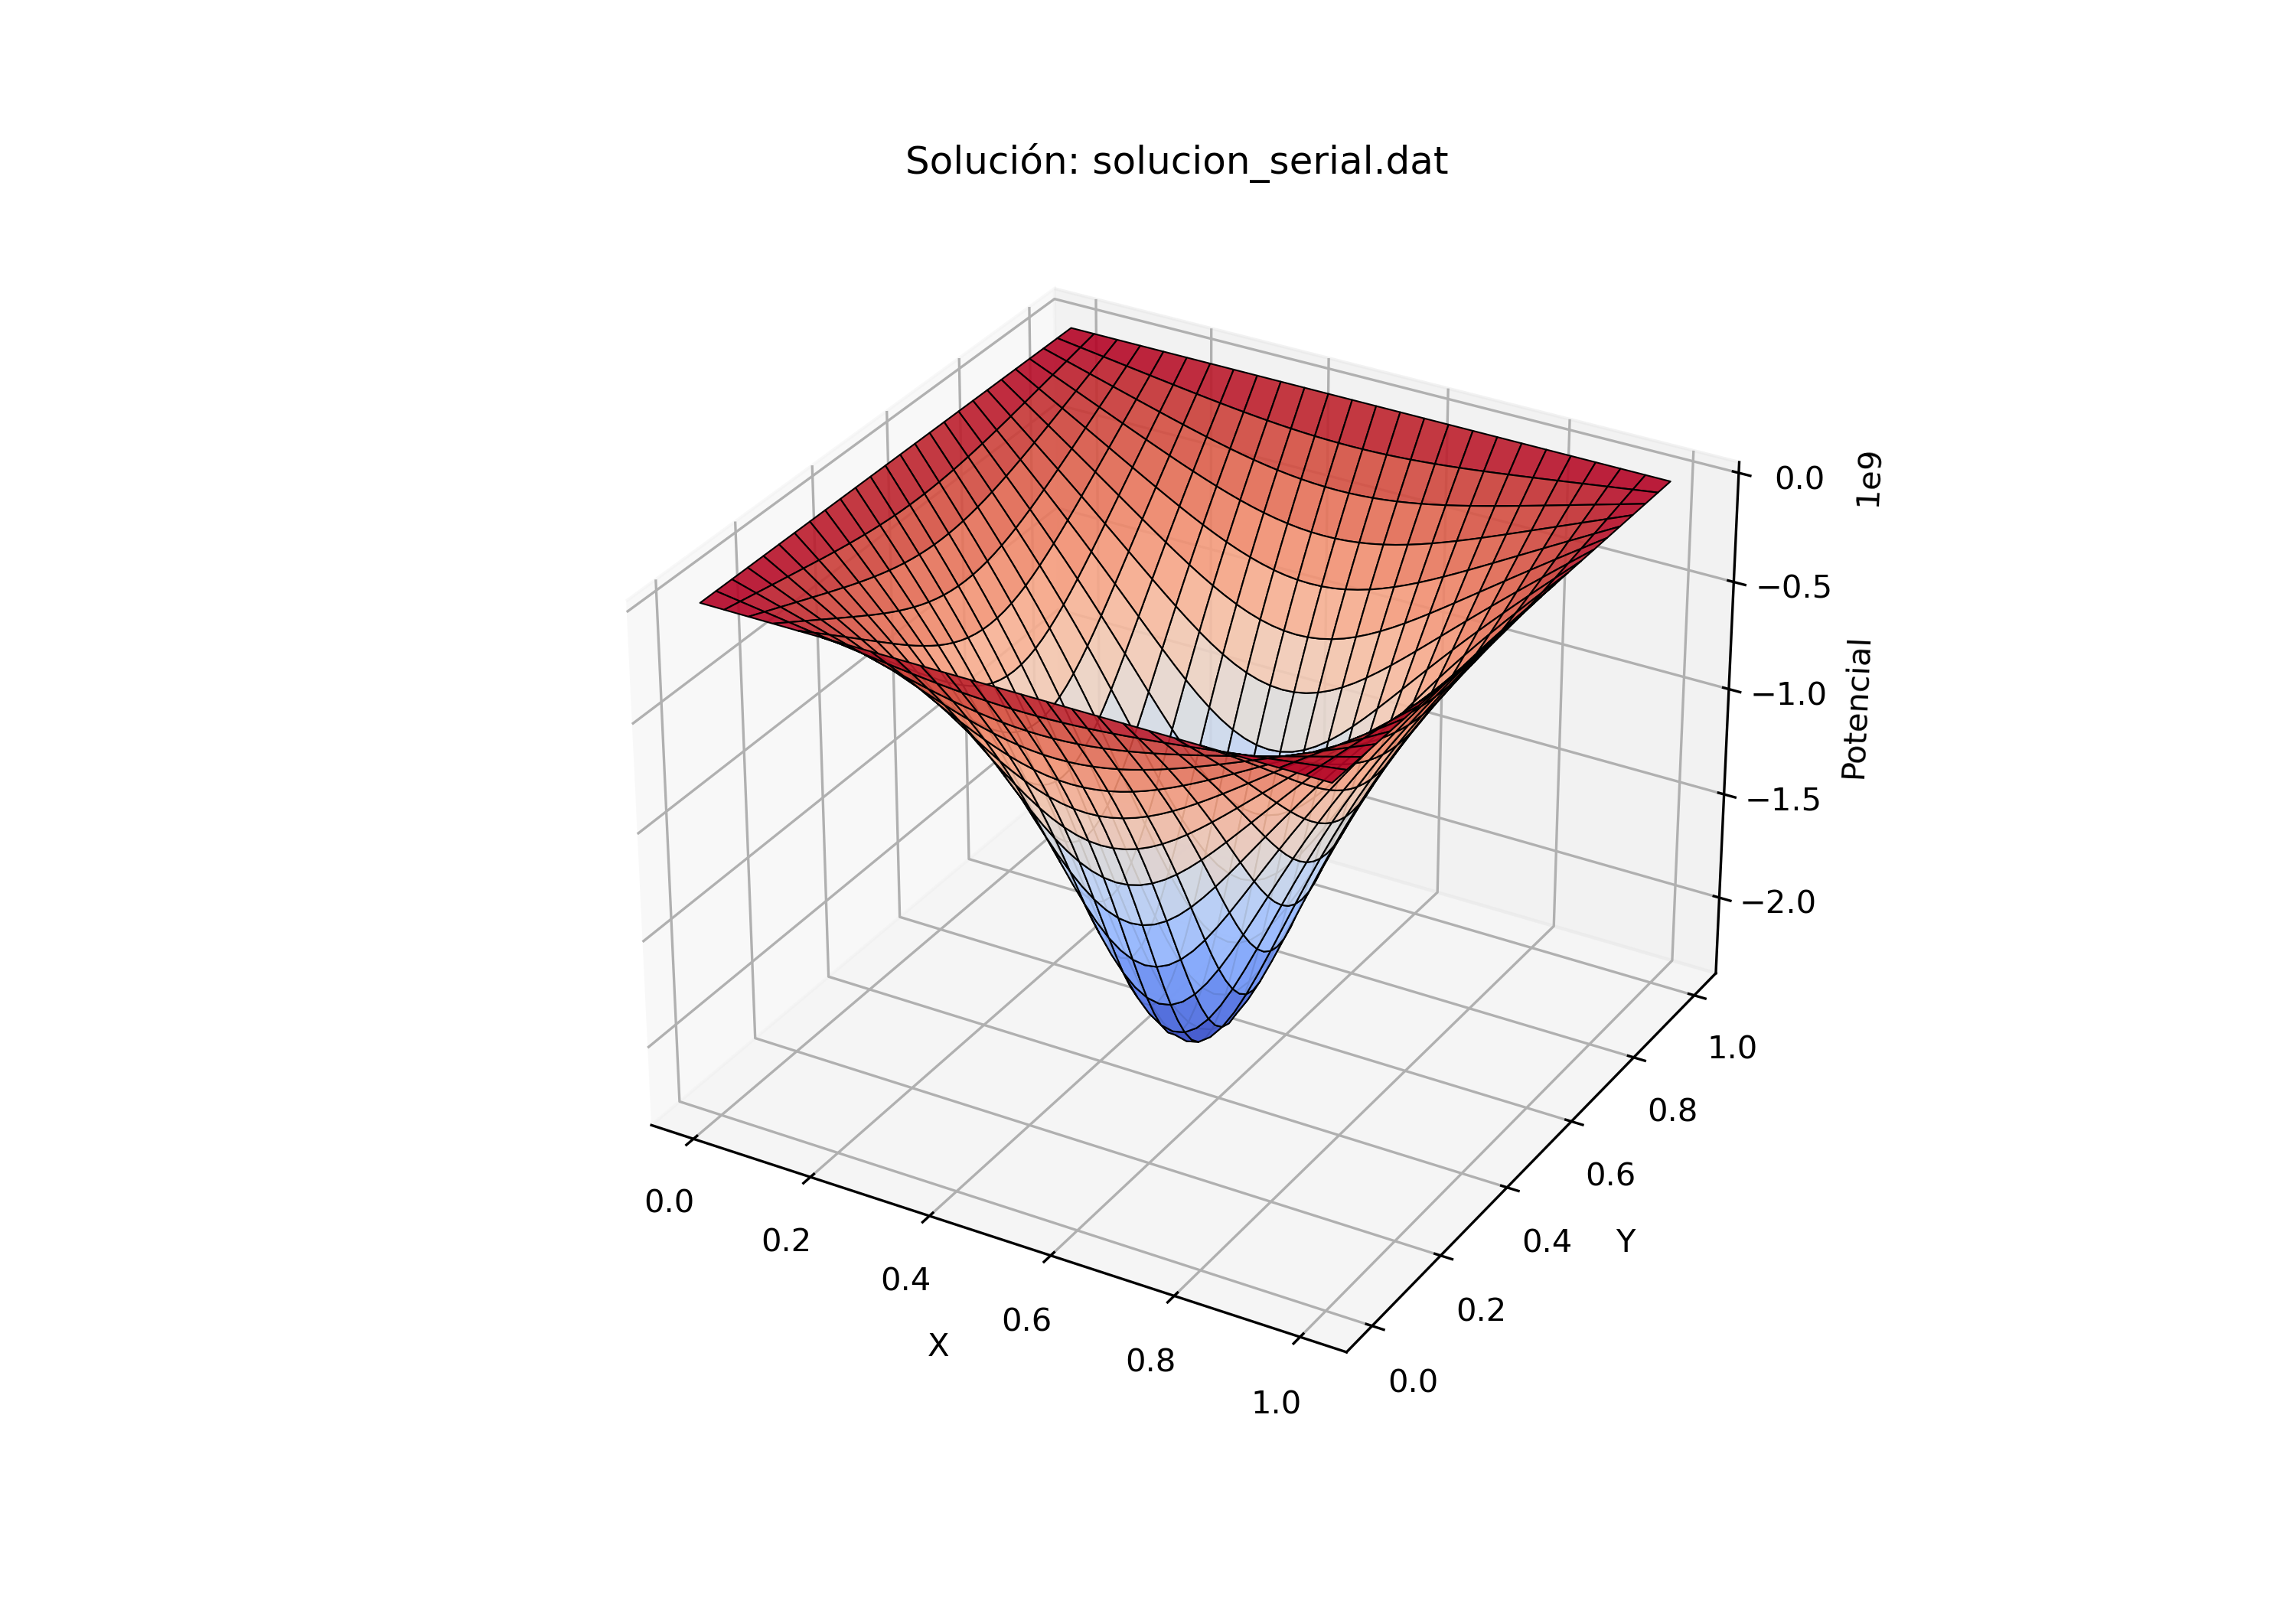
\includegraphics[width=0.8\textwidth]{imag/solucion_serial.png}
    \caption{Perfil de distribución de potencial obtenido con la versión Serial.}
\end{figure}

\begin{figure}[H]
    \centering
    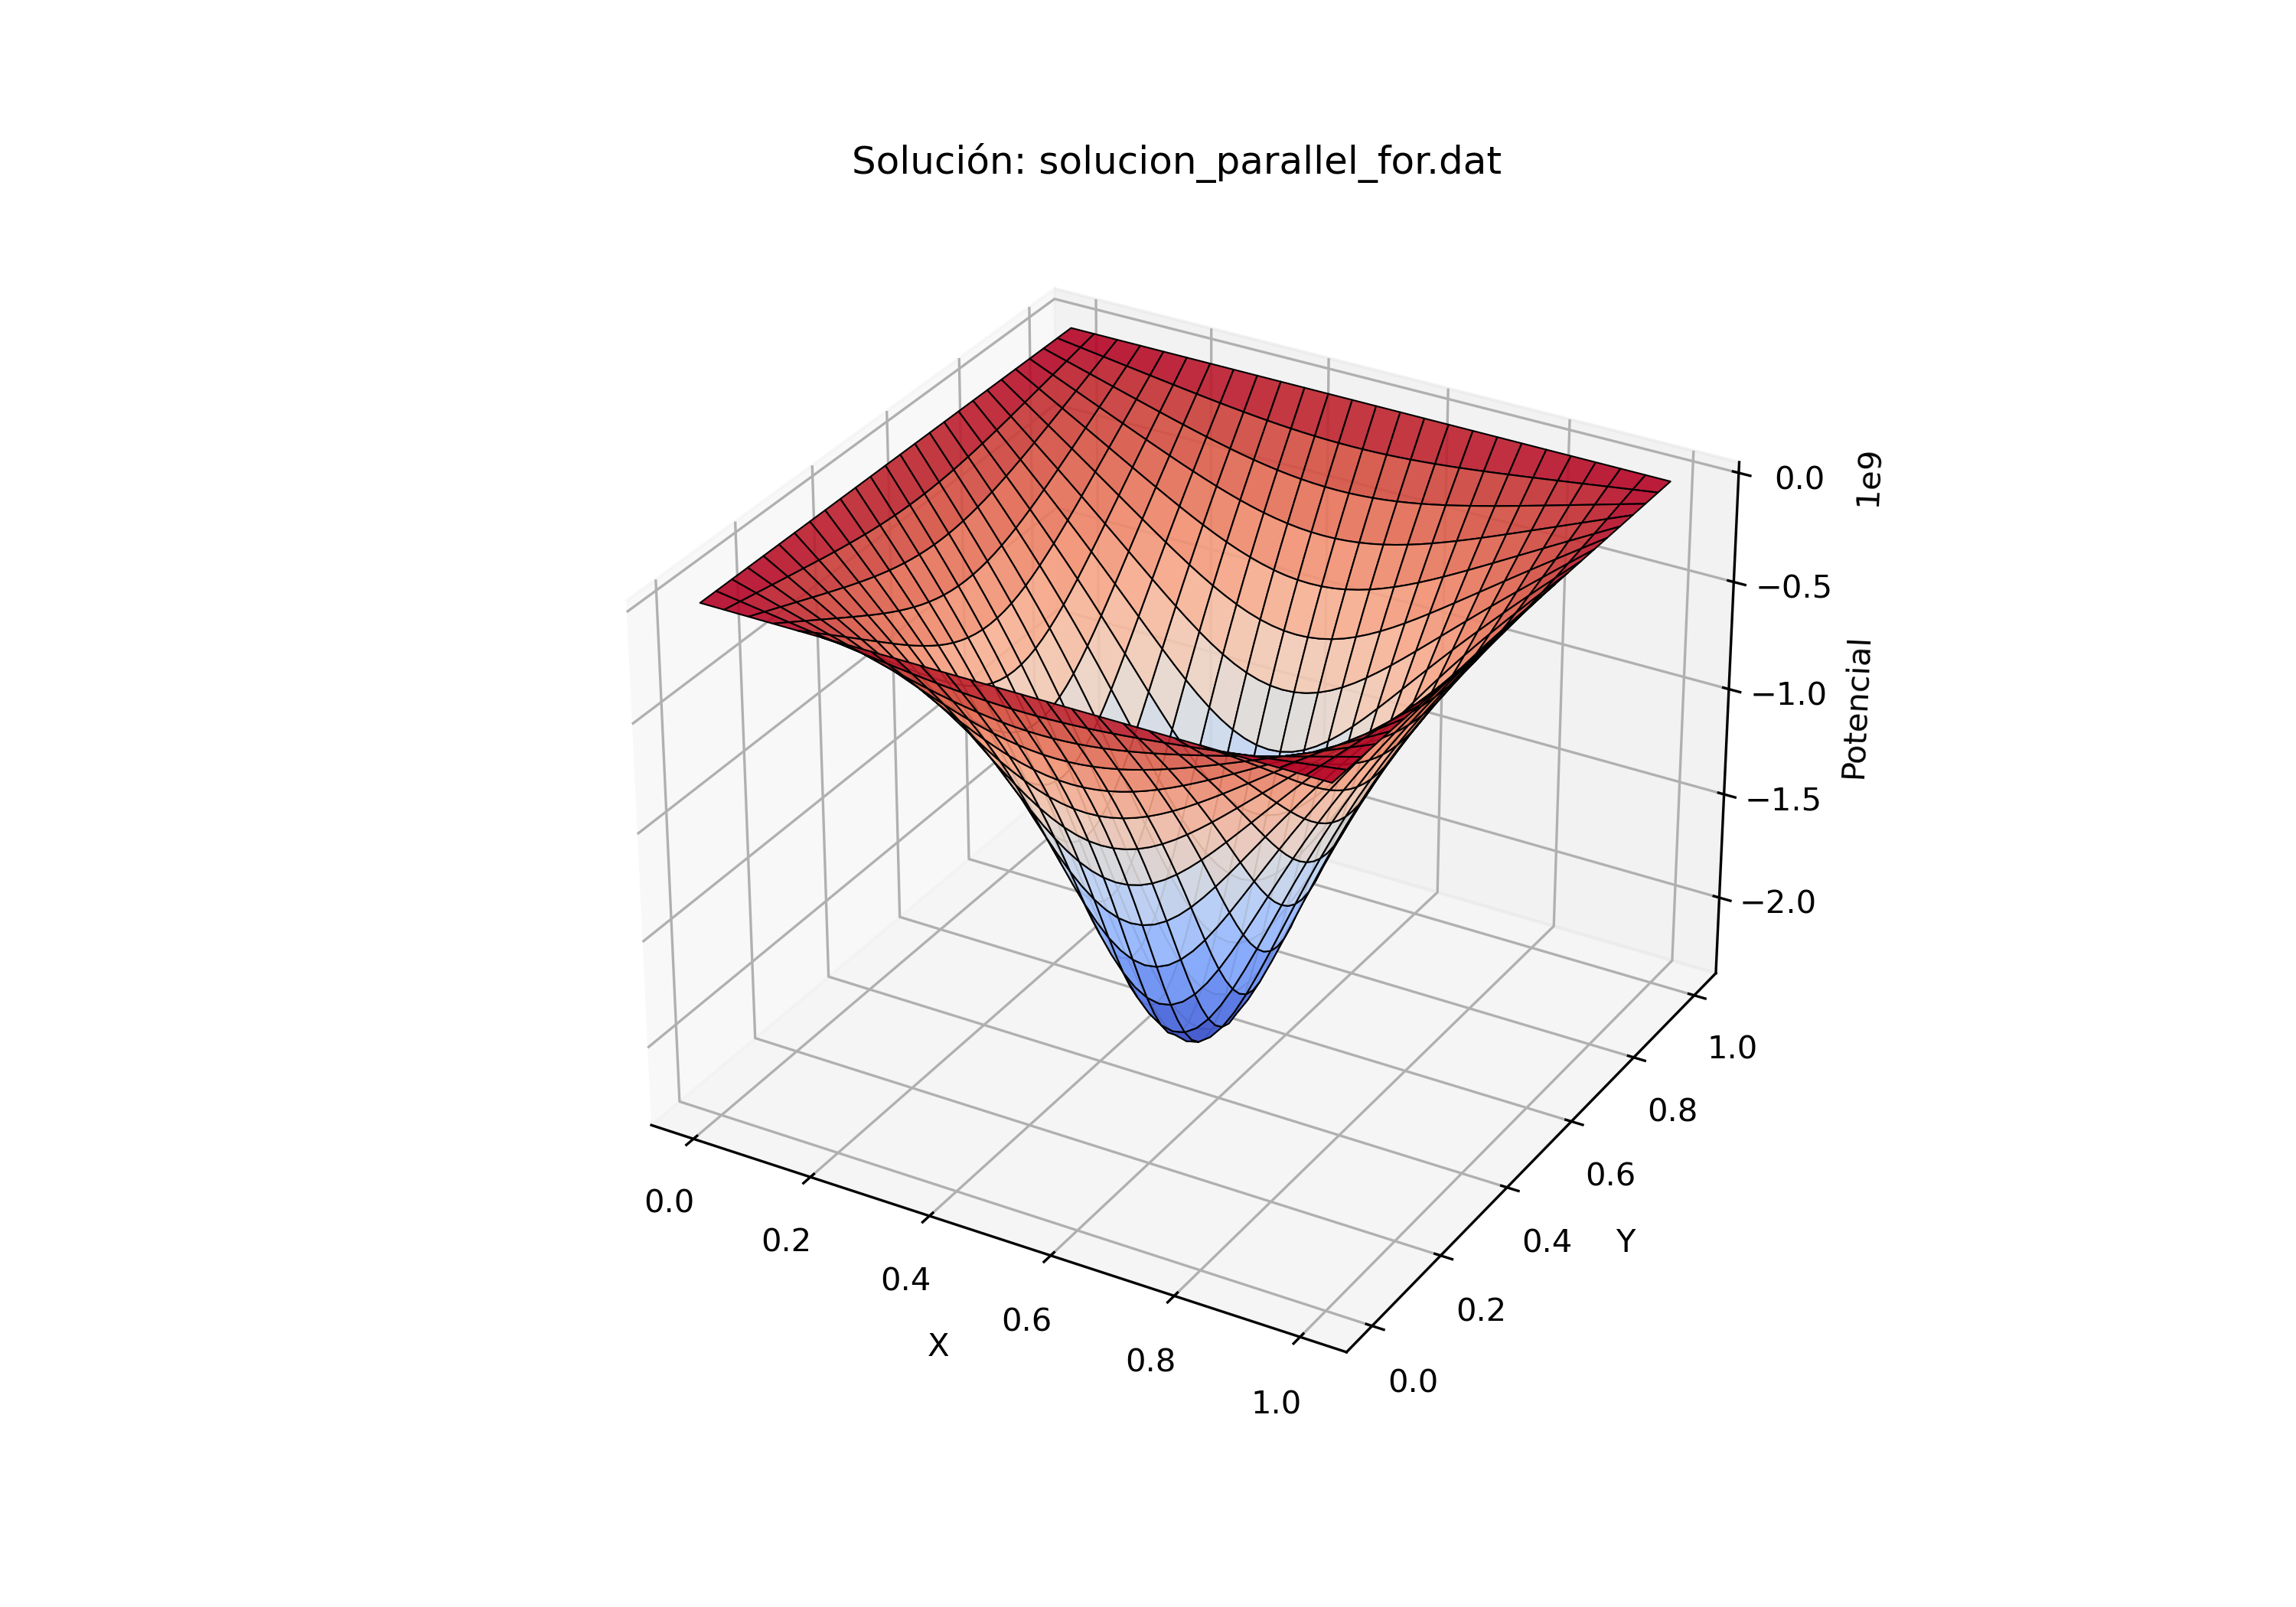
\includegraphics[width=0.8\textwidth]{imag/solucion_parallel_for.png}
    \caption{Perfil de distribución de potencial obtenido mediante paralelización con \texttt{collapse(2)}.}
\end{figure}

\begin{figure}[H]
    \centering
    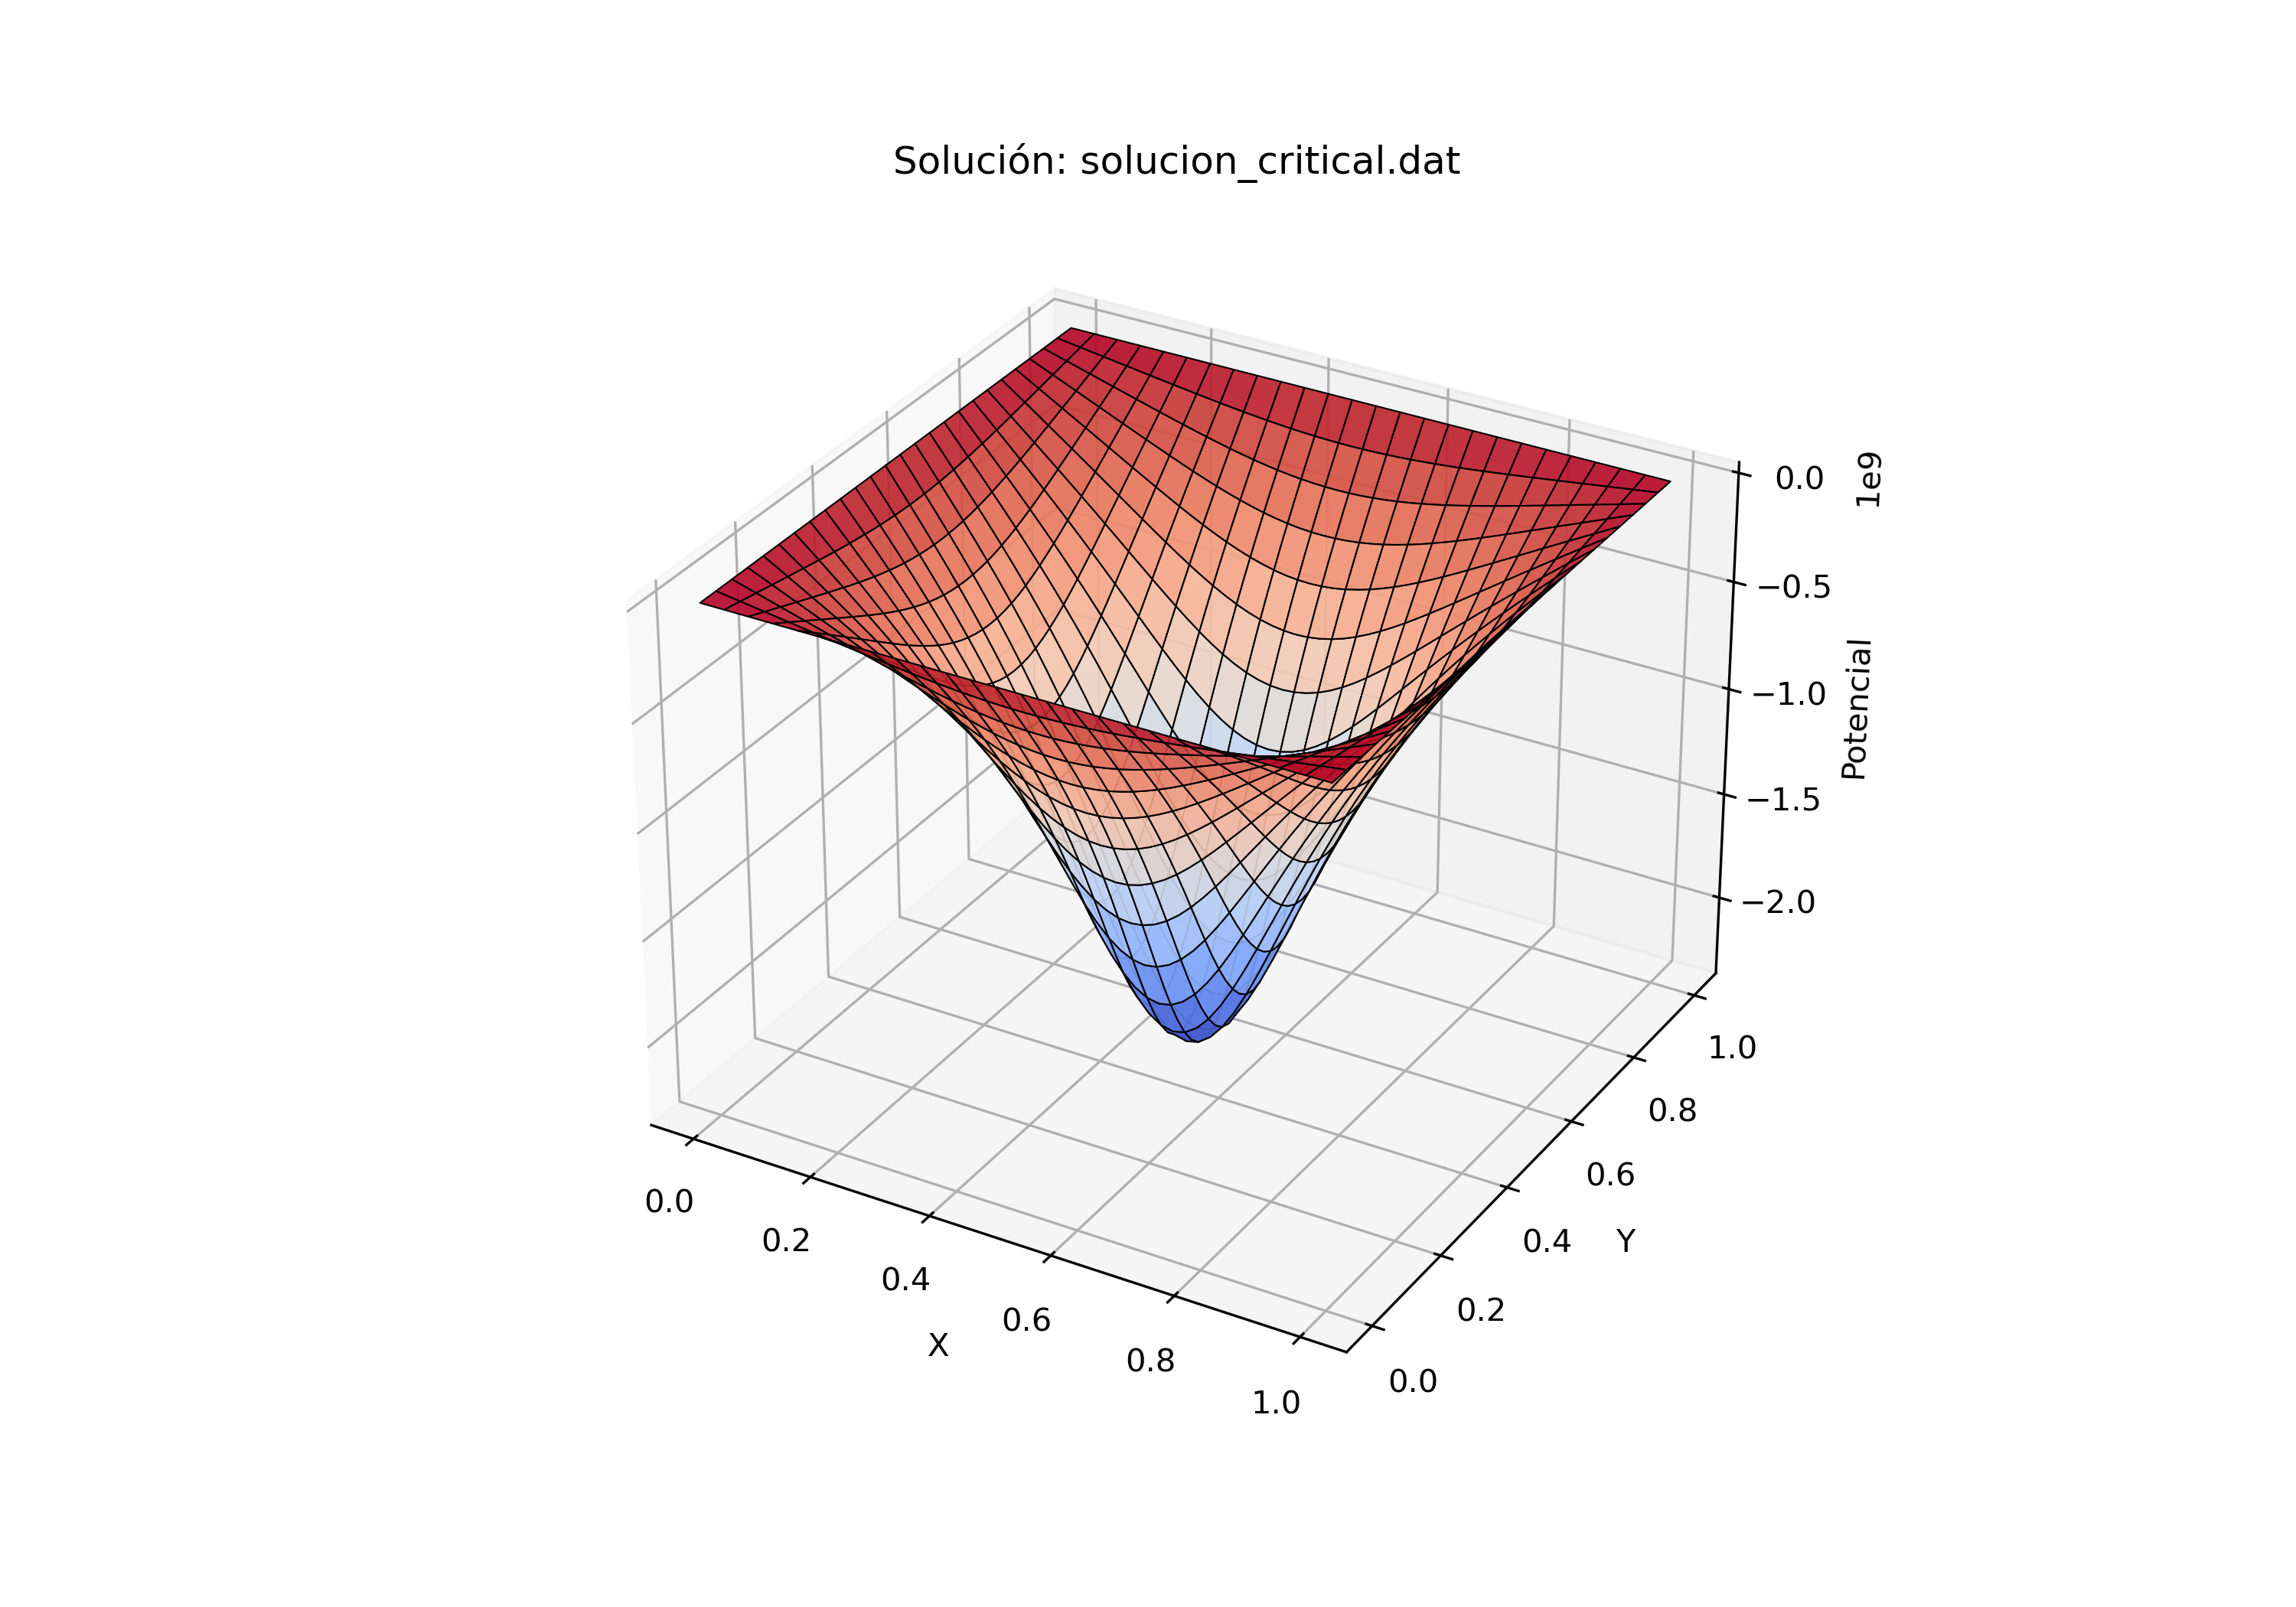
\includegraphics[width=0.8\textwidth]{imag/solucion_critical.png}
    \caption{Perfil de distribución de potencial obtenido utilizando una sección \texttt{critical}.}
\end{figure}

\begin{figure}[H]
    \centering
    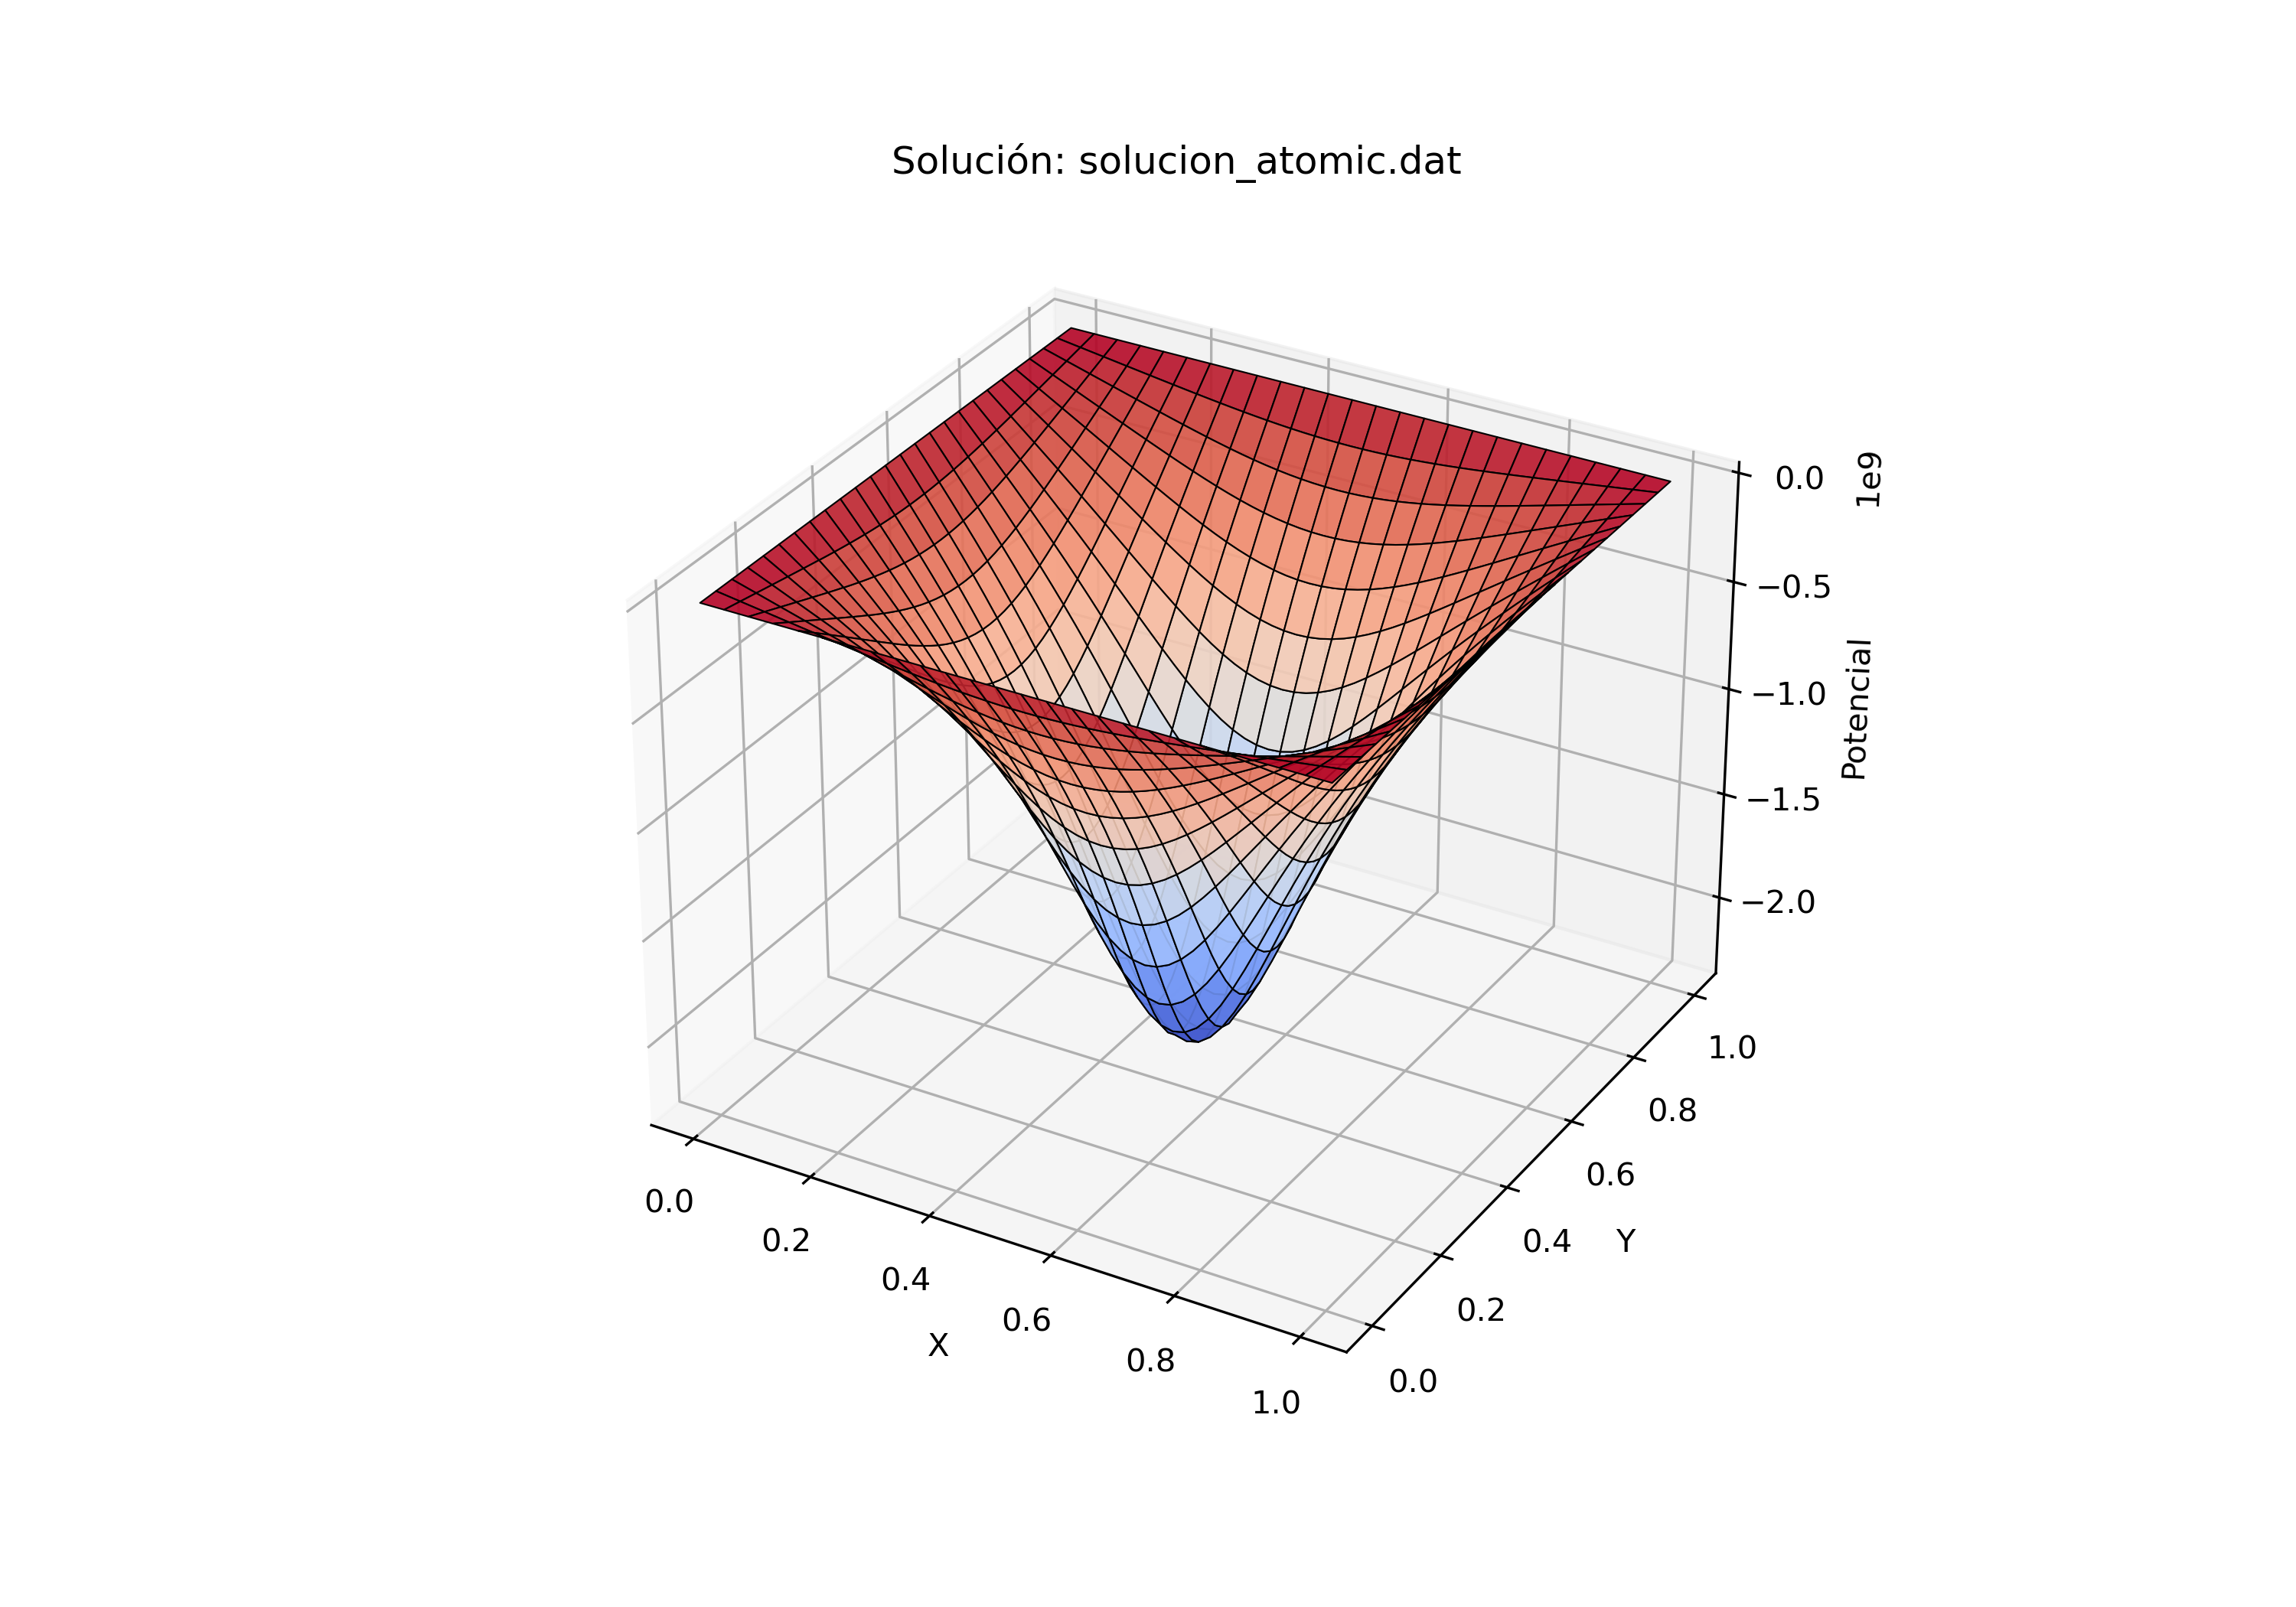
\includegraphics[width=0.8\textwidth]{imag/solucion_atomic.png}
    \caption{Perfil de distribución de potencial obtenido utilizando control \texttt{atomic}.}
\end{figure}

\begin{figure}[H]
    \centering
    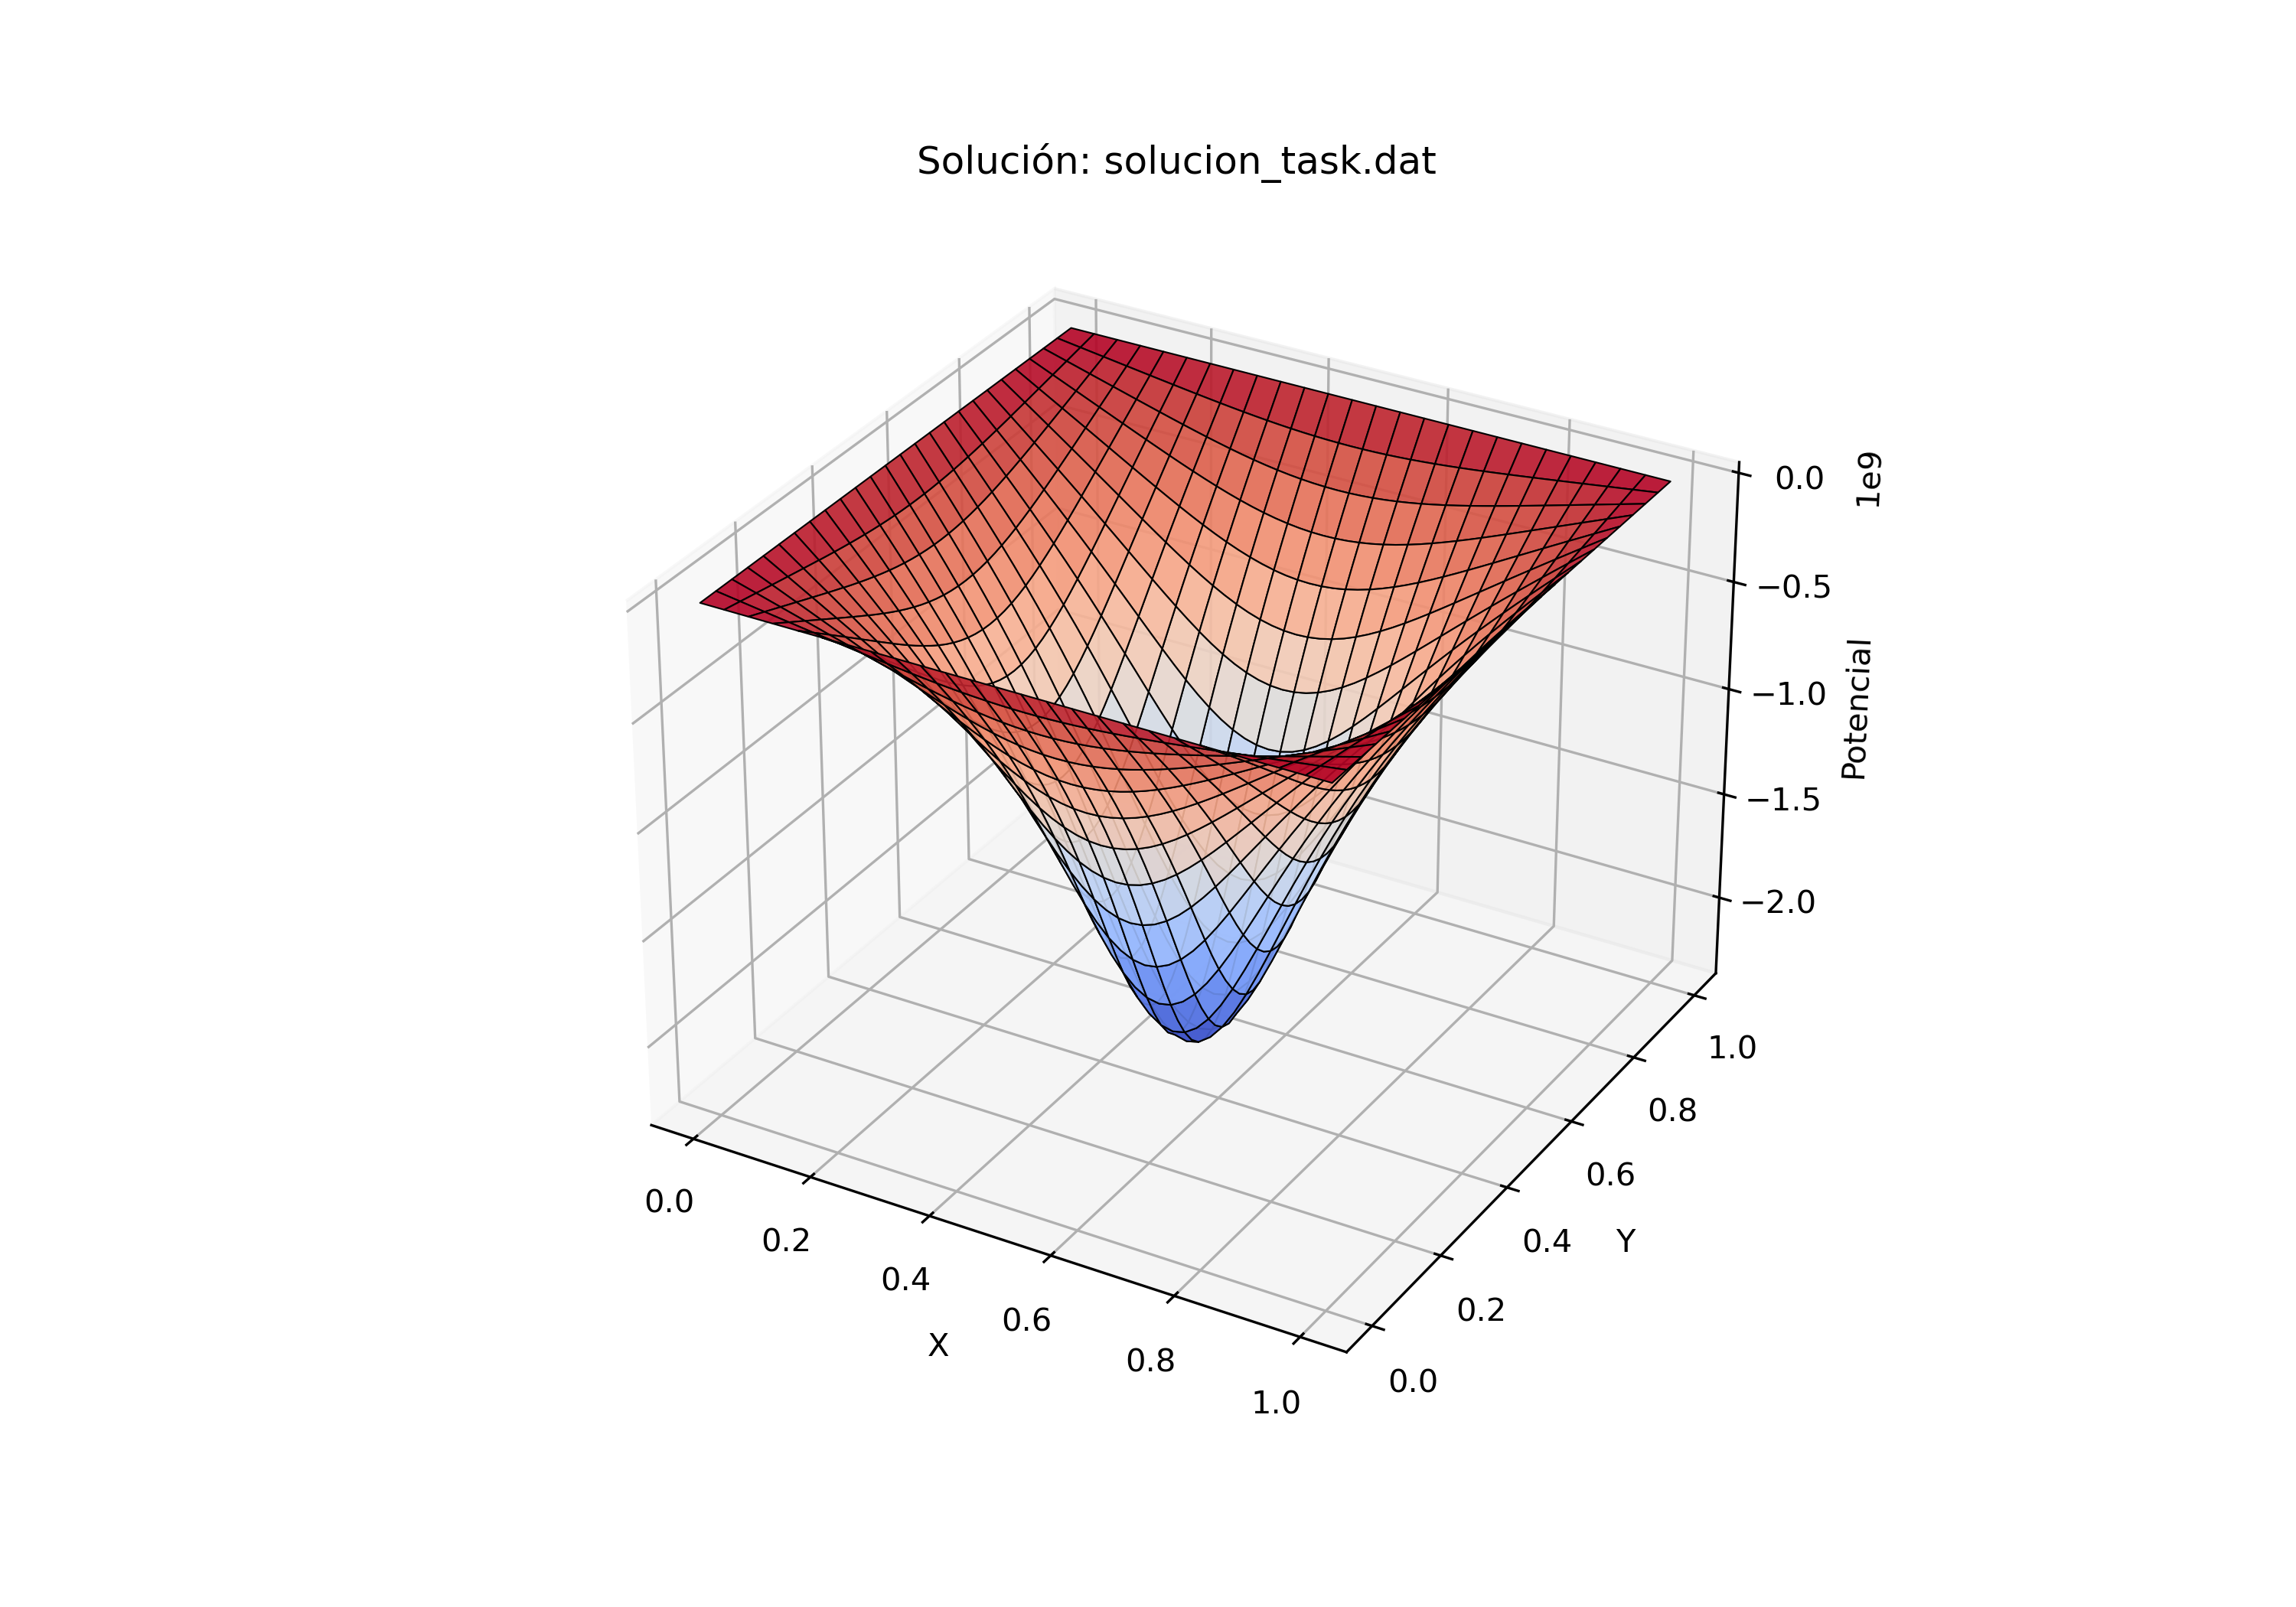
\includegraphics[width=0.8\textwidth]{imag/solucion_task.png}
    \caption{Perfil de distribución de potencial obtenido mediante el enfoque orientado a tareas (\texttt{task}).}
\end{figure}

\section{Resolución Multiproblema de la Ecuación de Poisson}

Para cumplir con los requerimientos de los ejercicios propuestos, en los cuales se exige resolver la ecuación de Poisson bajo cuatro condiciones de frontera y dominios distintos, se procedió a refactorizar la estructura del proyecto. 

En lugar de duplicar el código C++ para cada problema, se creó una cabecera auxiliar (\texttt{utils.h}) que centraliza las funciones matemáticas. Este enfoque modular permite que cada ejecutable itere automáticamente sobre los cuatro problemas, calcule las mallas numéricas y evalúe el error analítico sin alterar la lógica de las directivas OpenMP.

\subsection{Cabecera Auxiliar Matemática (\texttt{utils.h})}
En este archivo se definen los cuatro dominios espaciales, las soluciones analíticas exactas (que operan como condiciones de frontera de Dirichlet en los bordes) y el término fuente $f(x,y)$ correspondiente al Laplaciano de cada función. Adicionalmente, incluye una protección para evitar que el sistema exporte archivos de datos masivos cuando se ejecutan pruebas de estrés (\texttt{M > 1000}) en el clúster.

\begin{lstlisting}[language=C++, caption=Cabecera \texttt{utils.h} para la gestión de las cuatro ecuaciones diferenciales.]
#ifndef UTILS_H
#define UTILS_H

#include <iostream>
#include <vector>
#include <cmath>
#include <algorithm>
#include <fstream>
#include <string>

// Permite modificar la malla desde la compilación (Bash)
#ifndef VALOR_M
#define VALOR_M 50
#endif
#ifndef VALOR_N
#define VALOR_N 50
#endif

// Tolerancia estricta
const double TOL = 1e-7; 

// Obtiene los límites del dominio según el ejemplo
void get_domain(int ex, double& x_0, double& x_f, double& y_0, double& y_f) {
    if (ex == 1) { x_0=0.0; x_f=2.0; y_0=0.0; y_f=1.0; }
    else if (ex == 2) { x_0=1.0; x_f=2.0; y_0=0.0; y_f=1.0; }
    else if (ex == 3) { x_0=1.0; x_f=2.0; y_0=0.0; y_f=2.0; }
    else if (ex == 4) { x_0=1.0; x_f=2.0; y_0=1.0; y_f=2.0; }
    else { x_0=0.0; x_f=1.0; y_0=0.0; y_f=1.0; } // Fallback de seguridad
}

// Soluciones analíticas exactas (Condiciones de frontera)
double exact_sol(int ex, double x, double y) {
    if (ex == 1) return std::exp(x * y);
    if (ex == 2) return std::log(x * x + y * y);
    if (ex == 3) return (x - y) * (x - y);
    if (ex == 4) return x * y * std::log(x * y);
    return 0.0;
}

// Funciones fuente (Lado derecho de la Ecuación de Poisson)
double source_func(int ex, double x, double y) {
    if (ex == 1) return (x * x + y * y) * std::exp(x * y);
    if (ex == 2) return 0.0;
    if (ex == 3) return 4.0;
    if (ex == 4) return (x / y) + (y / x);
    return 0.0;
}

void initialize_grid(int ex, int M, int N, std::vector<std::vector<double>>& T, double& h, double& k) {
    double x_0 = 0.0, x_f = 0.0, y_0 = 0.0, y_f = 0.0; // Inicializadas
    get_domain(ex, x_0, x_f, y_0, y_f);
    h = (x_f - x_0) / M;
    k = (y_f - y_0) / N;

    T.assign(M + 1, std::vector<double>(N + 1, 0.0));
    
    // Condiciones de frontera exactas
    for (int j = 0; j <= N; ++j) {
        T[0][j] = exact_sol(ex, x_0, y_0 + j * k);
        T[M][j] = exact_sol(ex, x_f, y_0 + j * k);
    }
    for (int i = 0; i <= M; ++i) {
        T[i][0] = exact_sol(ex, x_0 + i * h, y_0);
        T[i][N] = exact_sol(ex, x_0 + i * h, y_f);
    }
}

void get_source_matrix(int ex, int M, int N, std::vector<std::vector<double>>& source, double h, double k) {
    double x_0 = 0.0, x_f = 0.0, y_0 = 0.0, y_f = 0.0; // Inicializadas
    get_domain(ex, x_0, x_f, y_0, y_f);
    source.assign(M + 1, std::vector<double>(N + 1, 0.0));
    for (int i = 0; i <= M; ++i) {
        for (int j = 0; j <= N; ++j) {
            source[i][j] = source_func(ex, x_0 + i * h, y_0 + j * k);
        }
    }
}

void export_to_file(int ex, const std::vector<std::vector<double>>& T, double h, double k, int M, int N, const std::string& method_name) {
    // PROTECCIÓN PARA EL CLÚSTER
    if (M > 1000) return; 

    double x_0 = 0.0, x_f = 0.0, y_0 = 0.0, y_f = 0.0; 
    get_domain(ex, x_0, x_f, y_0, y_f);
    
    std::string filename = "data/solucion_" + method_name + "_Ej" + std::to_string(ex) + ".dat";
    std::ofstream file(filename);
    if (!file.is_open()) return;
    
    for (int i = 0; i <= M; ++i) {
        for (int j = 0; j <= N; ++j) {
            file << (x_0 + i * h) << "\t" << (y_0 + j * k) << "\t" << T[i][j] << "\n";
        }
    }
    file.close();
}
#endif
\end{lstlisting}

\subsection{Implementaciones Multiproblema en C++}

Los códigos principales se ajustaron para delegar la inicialización a \texttt{utils.h}. Cada \texttt{main()} ahora recorre los cuatro ejercicios propuestos, ejecutando el algoritmo matemático subyacente de cada estrategia de paralelización.

\subsubsection{Implementación: Atomic}
\begin{lstlisting}[language=C++, caption=Versión iterativa con \texttt{\#pragma omp atomic}.]
#include "utils.h"
#include <omp.h>

void solve_poisson(std::vector<std::vector<double>>& T, const std::vector<std::vector<double>>& source, int M, int N, double h, double k, int ex) {
    double delta = 1.0;
    int iterations = 0;
    while (delta > TOL) {
        delta = 0.0;
        #pragma omp parallel for collapse(2) reduction(max:delta)
        for (int i = 1; i < M; ++i) {
            for (int j = 1; j < N; ++j) {
                double T_new = (((T[i+1][j] + T[i-1][j]) * k*k) + ((T[i][j+1] + T[i][j-1]) * h*h) - (source[i][j] * h*h * k*k)) / (2.0 * (h*h + k*k));
                delta = std::max(delta, std::abs(T_new - T[i][j]));
                T[i][j] = T_new;
            }
        }
        #pragma omp atomic
        iterations++;
    }
    if(M <= 1000) std::cout << "Ej " << ex << " Iteraciones (Atomic): " << iterations << std::endl;
}

int main() {
    int M = VALOR_M, N = VALOR_N;
    for (int ex = 1; ex <= 4; ++ex) {
        std::vector<std::vector<double>> T, source; double h, k;
        initialize_grid(ex, M, N, T, h, k); get_source_matrix(ex, M, N, source, h, k);
        solve_poisson(T, source, M, N, h, k, ex);
        export_to_file(ex, T, h, k, M, N, "atomic");
    }
    return 0;
}
\end{lstlisting}

\subsubsection{Implementación: Critical}
\begin{lstlisting}[language=C++, caption=Versión iterativa con \texttt{\#pragma omp critical}.]
#include "utils.h"
#include <omp.h>

void solve_poisson(std::vector<std::vector<double>>& T, const std::vector<std::vector<double>>& source, int M, int N, double h, double k, int ex) {
    double delta = 1.0;
    int iterations = 0;
    while (delta > TOL) {
        delta = 0.0;
        #pragma omp parallel for collapse(2) reduction(max:delta)
        for (int i = 1; i < M; ++i) {
            for (int j = 1; j < N; ++j) {
                double T_new = (((T[i+1][j] + T[i-1][j]) * k*k) + ((T[i][j+1] + T[i][j-1]) * h*h) - (source[i][j] * h*h * k*k)) / (2.0 * (h*h + k*k));
                delta = std::max(delta, std::abs(T_new - T[i][j]));
                T[i][j] = T_new;
            }
        }
        #pragma omp critical
        { iterations++; }
    }
    if(M <= 1000) std::cout << "Ej " << ex << " Iteraciones (Critical): " << iterations << std::endl;
}

int main() {
    int M = VALOR_M, N = VALOR_N;
    for (int ex = 1; ex <= 4; ++ex) {
        std::vector<std::vector<double>> T, source; double h, k;
        initialize_grid(ex, M, N, T, h, k); get_source_matrix(ex, M, N, source, h, k);
        solve_poisson(T, source, M, N, h, k, ex);
        export_to_file(ex, T, h, k, M, N, "critical");
    }
    return 0;
}
\end{lstlisting}

\subsubsection{Implementación: Parallel For}
\begin{lstlisting}[language=C++, caption=Versión con \texttt{\#pragma omp parallel for collapse(2)}.]
#include "utils.h"
#include <omp.h>

void solve_poisson(std::vector<std::vector<double>>& T, const std::vector<std::vector<double>>& source, int M, int N, double h, double k) {
    double delta = 1.0;
    while (delta > TOL) {
        delta = 0.0;
        #pragma omp parallel for collapse(2) reduction(max:delta)
        for (int i = 1; i < M; ++i) {
            for (int j = 1; j < N; ++j) {
                double T_new = (((T[i+1][j] + T[i-1][j]) * k*k) + ((T[i][j+1] + T[i][j-1]) * h*h) - (source[i][j] * h*h * k*k)) / (2.0 * (h*h + k*k));
                delta = std::max(delta, std::abs(T_new - T[i][j]));
                T[i][j] = T_new;
            }
        }
    }
}

int main() {
    int M = VALOR_M, N = VALOR_N;
    for (int ex = 1; ex <= 4; ++ex) {
        std::vector<std::vector<double>> T, source; double h, k;
        initialize_grid(ex, M, N, T, h, k);
        get_source_matrix(ex, M, N, source, h, k);
        solve_poisson(T, source, M, N, h, k);
        export_to_file(ex, T, h, k, M, N, "parallel_for");
    }
    return 0;
}
\end{lstlisting}

\subsubsection{Implementación: Serial}
\begin{lstlisting}[language=C++, caption=Versión secuencial base para métricas de aceleración.]
#include "utils.h"

void solve_poisson(std::vector<std::vector<double>>& T, const std::vector<std::vector<double>>& source, int M, int N, double h, double k) {
    double delta = 1.0;
    while (delta > TOL) {
        delta = 0.0;
        for (int i = 1; i < M; ++i) {
            for (int j = 1; j < N; ++j) {
                double T_new = (((T[i+1][j] + T[i-1][j]) * k*k) + ((T[i][j+1] + T[i][j-1]) * h*h) - (source[i][j] * h*h * k*k)) / (2.0 * (h*h + k*k));
                delta = std::max(delta, std::abs(T_new - T[i][j]));
                T[i][j] = T_new;
            }
        }
    }
}

int main() {
    int M = VALOR_M, N = VALOR_N;
    for (int ex = 1; ex <= 4; ++ex) {
        std::vector<std::vector<double>> T, source;
        double h, k;
        initialize_grid(ex, M, N, T, h, k);
        get_source_matrix(ex, M, N, source, h, k);
        solve_poisson(T, source, M, N, h, k);
        export_to_file(ex, T, h, k, M, N, "serial");
    }
    return 0;
}
\end{lstlisting}

\subsubsection{Implementación: Task}
\begin{lstlisting}[language=C++, caption=Versión basada en descomposición por tareas (\texttt{task}).]
#include "utils.h"
#include <omp.h>

void solve_poisson(std::vector<std::vector<double>>& T, const std::vector<std::vector<double>>& source, int M, int N, double h, double k) {
    double delta = 1.0;
    int block_size = std::max(10, M / 10); // Escala el bloque dinámicamente
    while (delta > TOL) {
        double max_delta = 0.0;
        #pragma omp parallel shared(max_delta)
        {
            #pragma omp single
            {
                for (int bi = 1; bi < M; bi += block_size) {
                    for (int bj = 1; bj < N; bj += block_size) {
                        #pragma omp task shared(max_delta)
                        {
                            double local_delta = 0.0;
                            for (int i = bi; i < std::min(bi + block_size, M); ++i) {
                                for (int j = bj; j < std::min(bj + block_size, N); ++j) {
                                    double T_new = (((T[i+1][j] + T[i-1][j]) * k*k) + ((T[i][j+1] + T[i][j-1]) * h*h) - (source[i][j] * h*h * k*k)) / (2.0 * (h*h + k*k));
                                    local_delta = std::max(local_delta, std::abs(T_new - T[i][j]));
                                    T[i][j] = T_new;
                                }
                            }
                            #pragma omp critical
                            { max_delta = std::max(max_delta, local_delta); }
                        }
                    }
                }
                #pragma omp taskwait
            }
        }
        delta = max_delta;
    }
}

int main() {
    int M = VALOR_M, N = VALOR_N;
    for (int ex = 1; ex <= 4; ++ex) {
        std::vector<std::vector<double>> T, source; double h, k;
        initialize_grid(ex, M, N, T, h, k); get_source_matrix(ex, M, N, source, h, k);
        solve_poisson(T, source, M, N, h, k);
        export_to_file(ex, T, h, k, M, N, "task");
    }
    return 0;
}
\end{lstlisting}

\subsection{Automatización: Benchmark y Gráficas}

El proceso se automatizó mediante un script \texttt{bash} que inyecta parámetros en el compilador C++, y un script de Python que genera gráficas superponiendo la solución analítica exacta (malla de líneas negras) sobre la solución numérica discretizada (puntos rojos).

\begin{lstlisting}[language=bash, caption=Script de Benchmark Dinámico para Clúster.]
#!/bin/bash

METODOS=("poisson_serial" "poisson_parallel_for" "poisson_critical" "poisson_atomic" "poisson_task")
TAMANOS=(50 250 500) # Para el clúster puedes cambiar a: (1000 2000 5000)
HILOS=(12 24 48 64)
LOG="benchmark_cluster_resultados.txt"

echo "Metodo,Hilos,N,Tiempo(s)" > $LOG

echo "Iniciando Benchmark Multihilo..."

# Limpiamos binarios previos
mkdir -p bin data imag
rm -f bin/*

for n in "${TAMANOS[@]}"; do
    echo "=========================================="
    echo "  Compilando para tamaño de Malla N=$n"
    echo "=========================================="
    
    # 1. Compilar todo con el nuevo tamaño inyectado por preprocesador
    for m in "${METODOS[@]}"; do
        g++ -std=c++17 -O3 -Wall -Wextra -fopenmp -Isrc -DVALOR_M=$n -DVALOR_N=$n "src/$m.cpp" -o "bin/$m"
    done

    # 2. Ejecutar variando el número de hilos
    for h in "${HILOS[@]}"; do
        export OMP_NUM_THREADS=$h
        echo "--- Probando con $h Hilos ---"
        
        for m in "${METODOS[@]}"; do
            if [[ "$m" == "poisson_serial" && "$h" != "${HILOS[0]}" ]]; then
                continue 
            fi

            echo -n "  Ejecutando $m ... "
            START=$(date +%s.%N)
            ./bin/$m
            END=$(date +%s.%N)
            
            DURACION=$(echo "$END - $START" | bc)
            echo "Hecho en $DURACION s"
            
            if [[ "$m" == "poisson_serial" ]]; then
                echo "$m,1,$n,$DURACION" >> $LOG
            else
                echo "$m,$h,$n,$DURACION" >> $LOG
            fi
        done
    done
done
echo "Benchmark completado. Revisa $LOG"
\end{lstlisting}

\begin{lstlisting}[language=Python, caption=Script de visualización analítica vs. numérica.]
import os
import numpy as np
import matplotlib.pyplot as plt
import glob

# Diccionario de soluciones analíticas según el ejemplo
def sol_analitica(ex, x, y):
    if ex == 1: return np.exp(x * y)
    if ex == 2: return np.log(x**2 + y**2)
    if ex == 3: return (x - y)**2
    if ex == 4: return x * y * np.log(x * y)
    return x*0

def plot_comparative_3d(filename, output_name):
    try:
        data = np.loadtxt(filename)
        if data.size == 0: return
        
        ex_num = 1
        for i in range(1, 5):
            if f"Ej{i}" in filename: ex_num = i
            
        x = data[:, 0]; y = data[:, 1]; z = data[:, 2]
        M = len(np.unique(x)); N = len(np.unique(y))
        X = x.reshape((M, N)); Y = y.reshape((M, N)); Z_num = z.reshape((M, N))

        Z_ana = sol_analitica(ex_num, X, Y)

        fig = plt.figure(figsize=(10, 7))
        ax = fig.add_subplot(111, projection='3d')
        
        # Malla negra para la solución analítica
        ax.plot_wireframe(X, Y, Z_ana, color='black', label='Solución analítica', linewidth=1)
        
        # Puntos rojos para la solución numérica
        ax.scatter(X, Y, Z_num, color='red', s=5, label='Solución numérica', alpha=0.8)

        ax.set_xlabel('X')
        ax.set_ylabel('Y')
        ax.set_zlabel('Potencial')
        ax.set_title(f'Ecuación de Poisson - Ejemplo {ex_num}')
        ax.legend()

        plt.savefig(output_name, dpi=300)
        plt.close()
        print(f"Gráfica guardada: {output_name}")
    except Exception as e:
        print(f"Error procesando {filename}: {e}")

if __name__ == '__main__':
    os.makedirs('imag', exist_ok=True)
    archivos = glob.glob('data/*.dat')
    for arc in archivos:
        salida = os.path.join('imag', os.path.basename(arc).replace('.dat', '.png'))
        plot_comparative_3d(arc, salida)
\end{lstlisting}

\subsection{Resultados Gráficos (Analítica vs Numérica)}

A continuación se presentan las 20 gráficas de las distribuciones obtenidas tras resolver los cuatro ejemplos matemáticos implementando los cinco métodos computacionales en estudio. En todas ellas se constata que la solución discretizada computacionalmente se ajusta de manera ideal a la malla analítica (exacta).

% === EJEMPLO 1 ===
\begin{figure}[H]
    \centering
    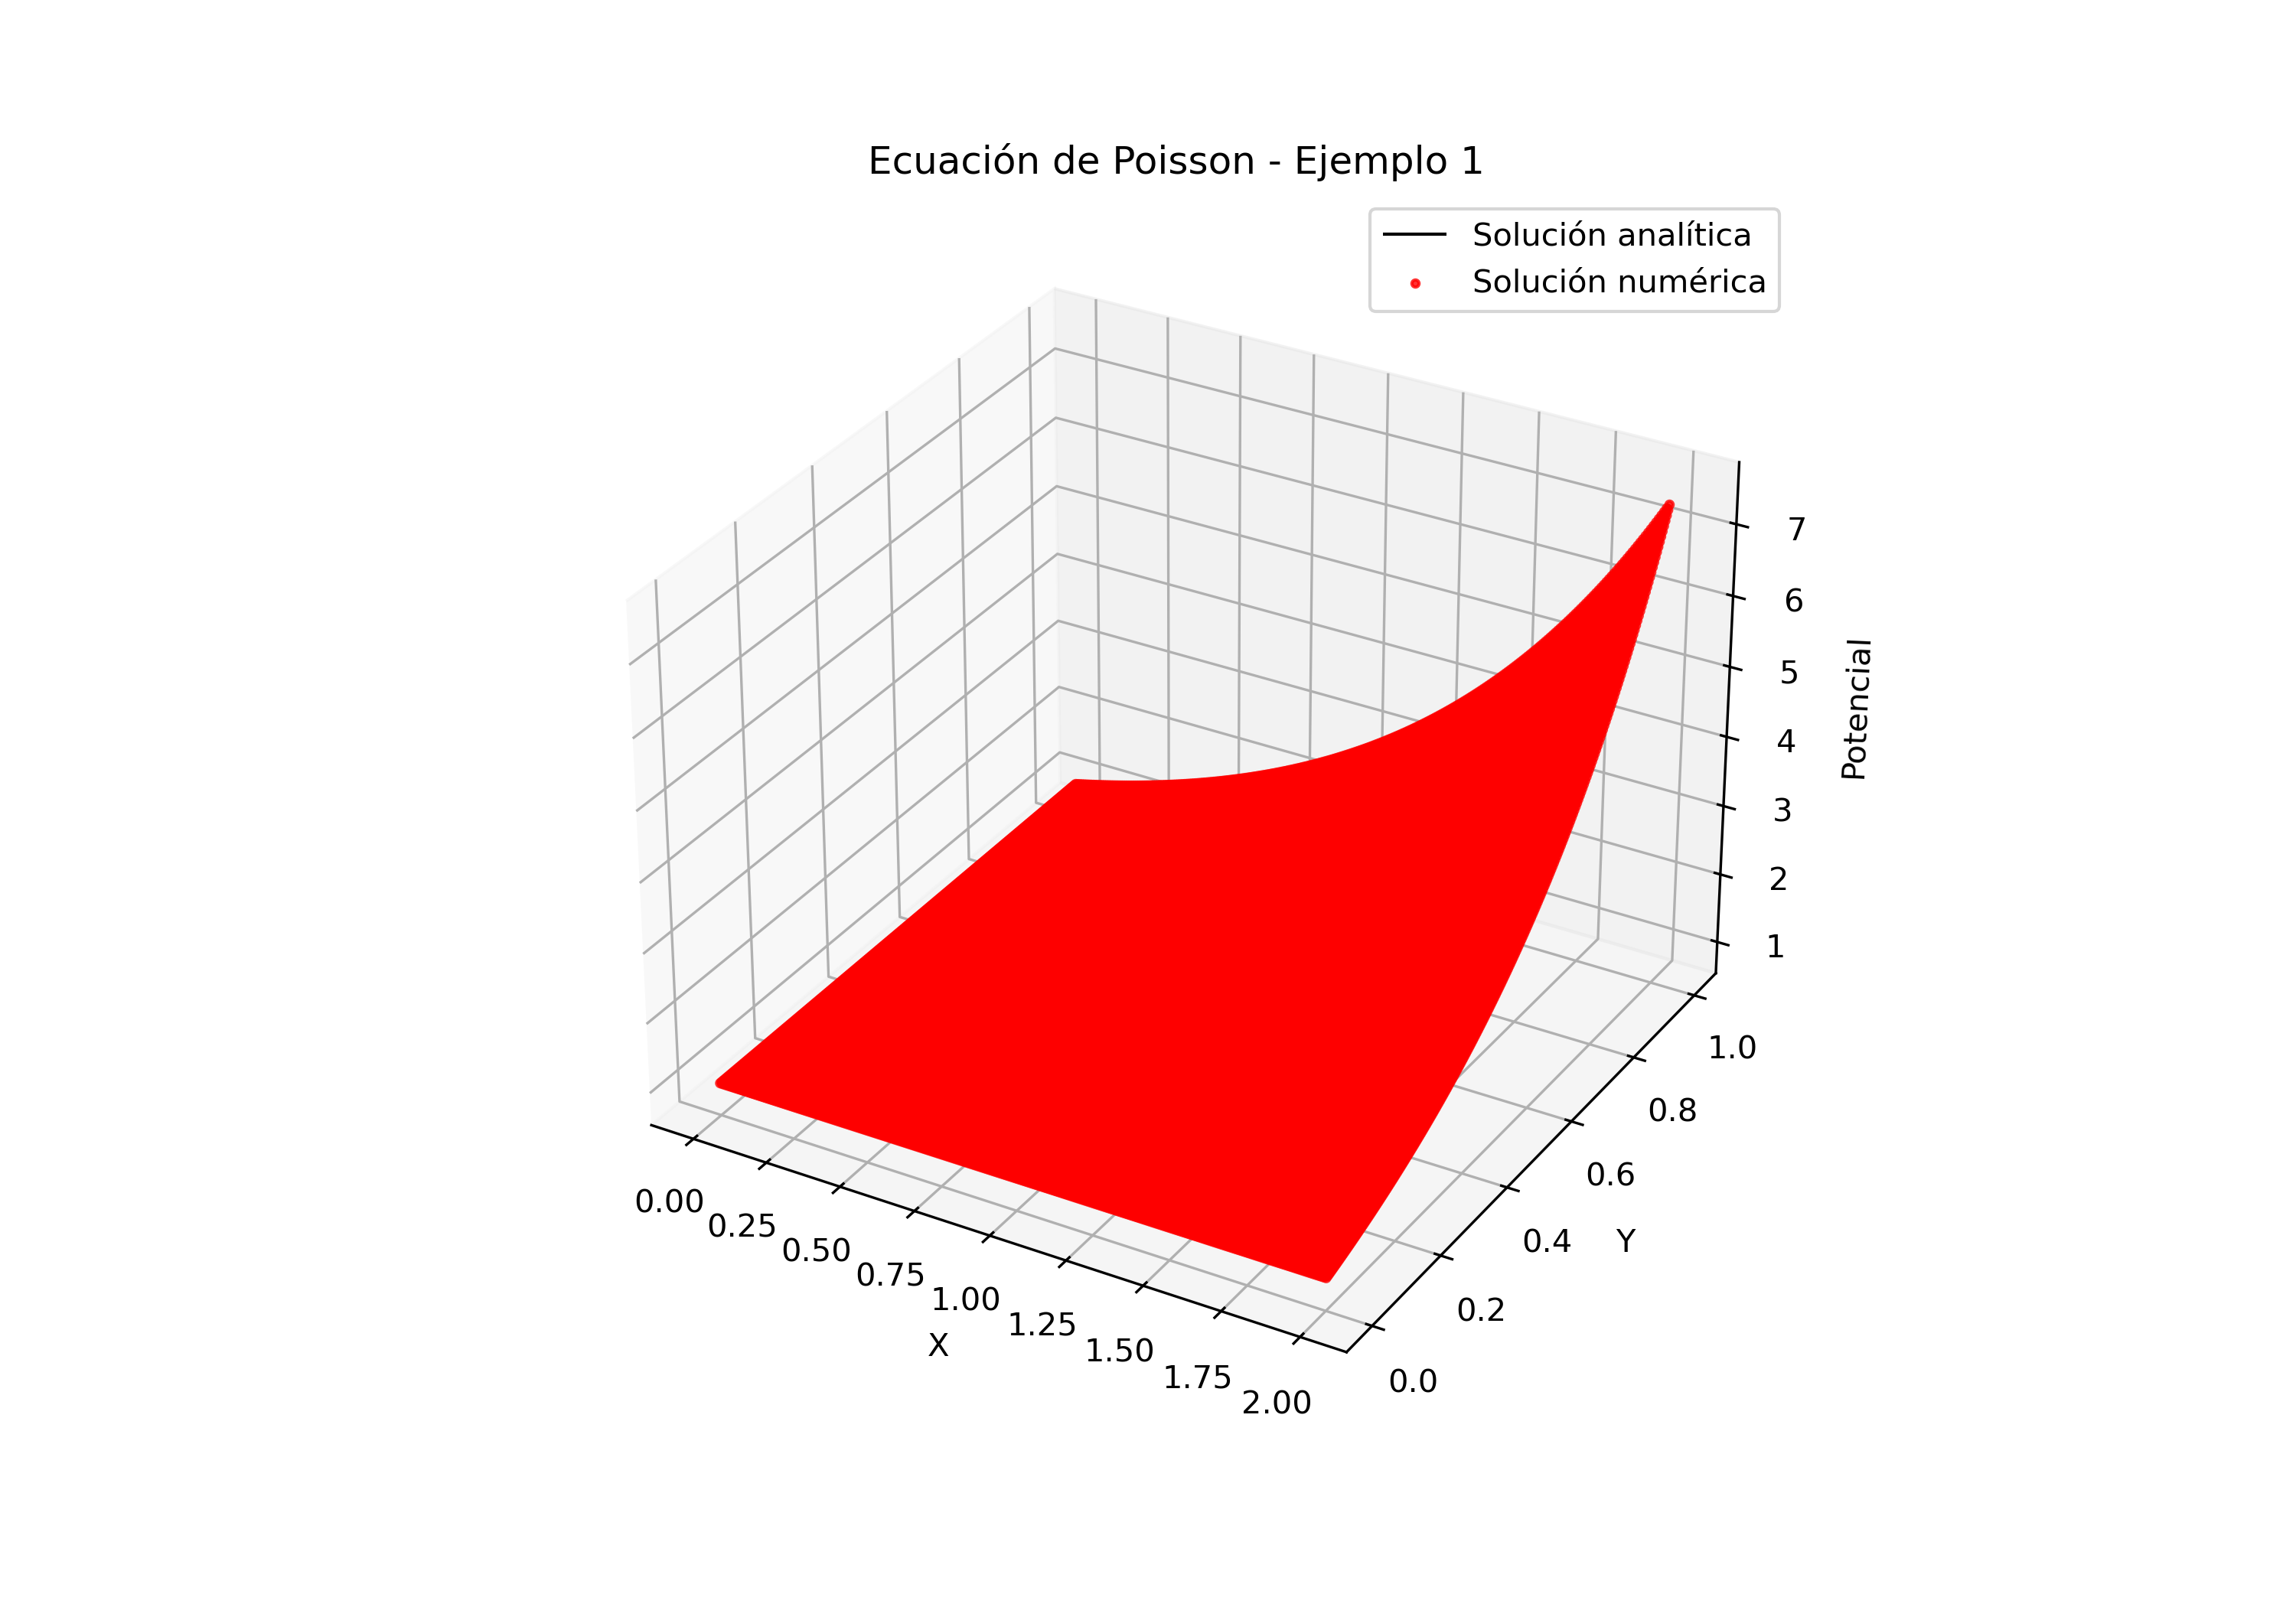
\includegraphics[width=0.8\textwidth]{imag/solucion_serial_Ej1.png}
    \caption{Ejemplo 1 resuelto con método secuencial.}
\end{figure}
\begin{figure}[H]
    \centering
    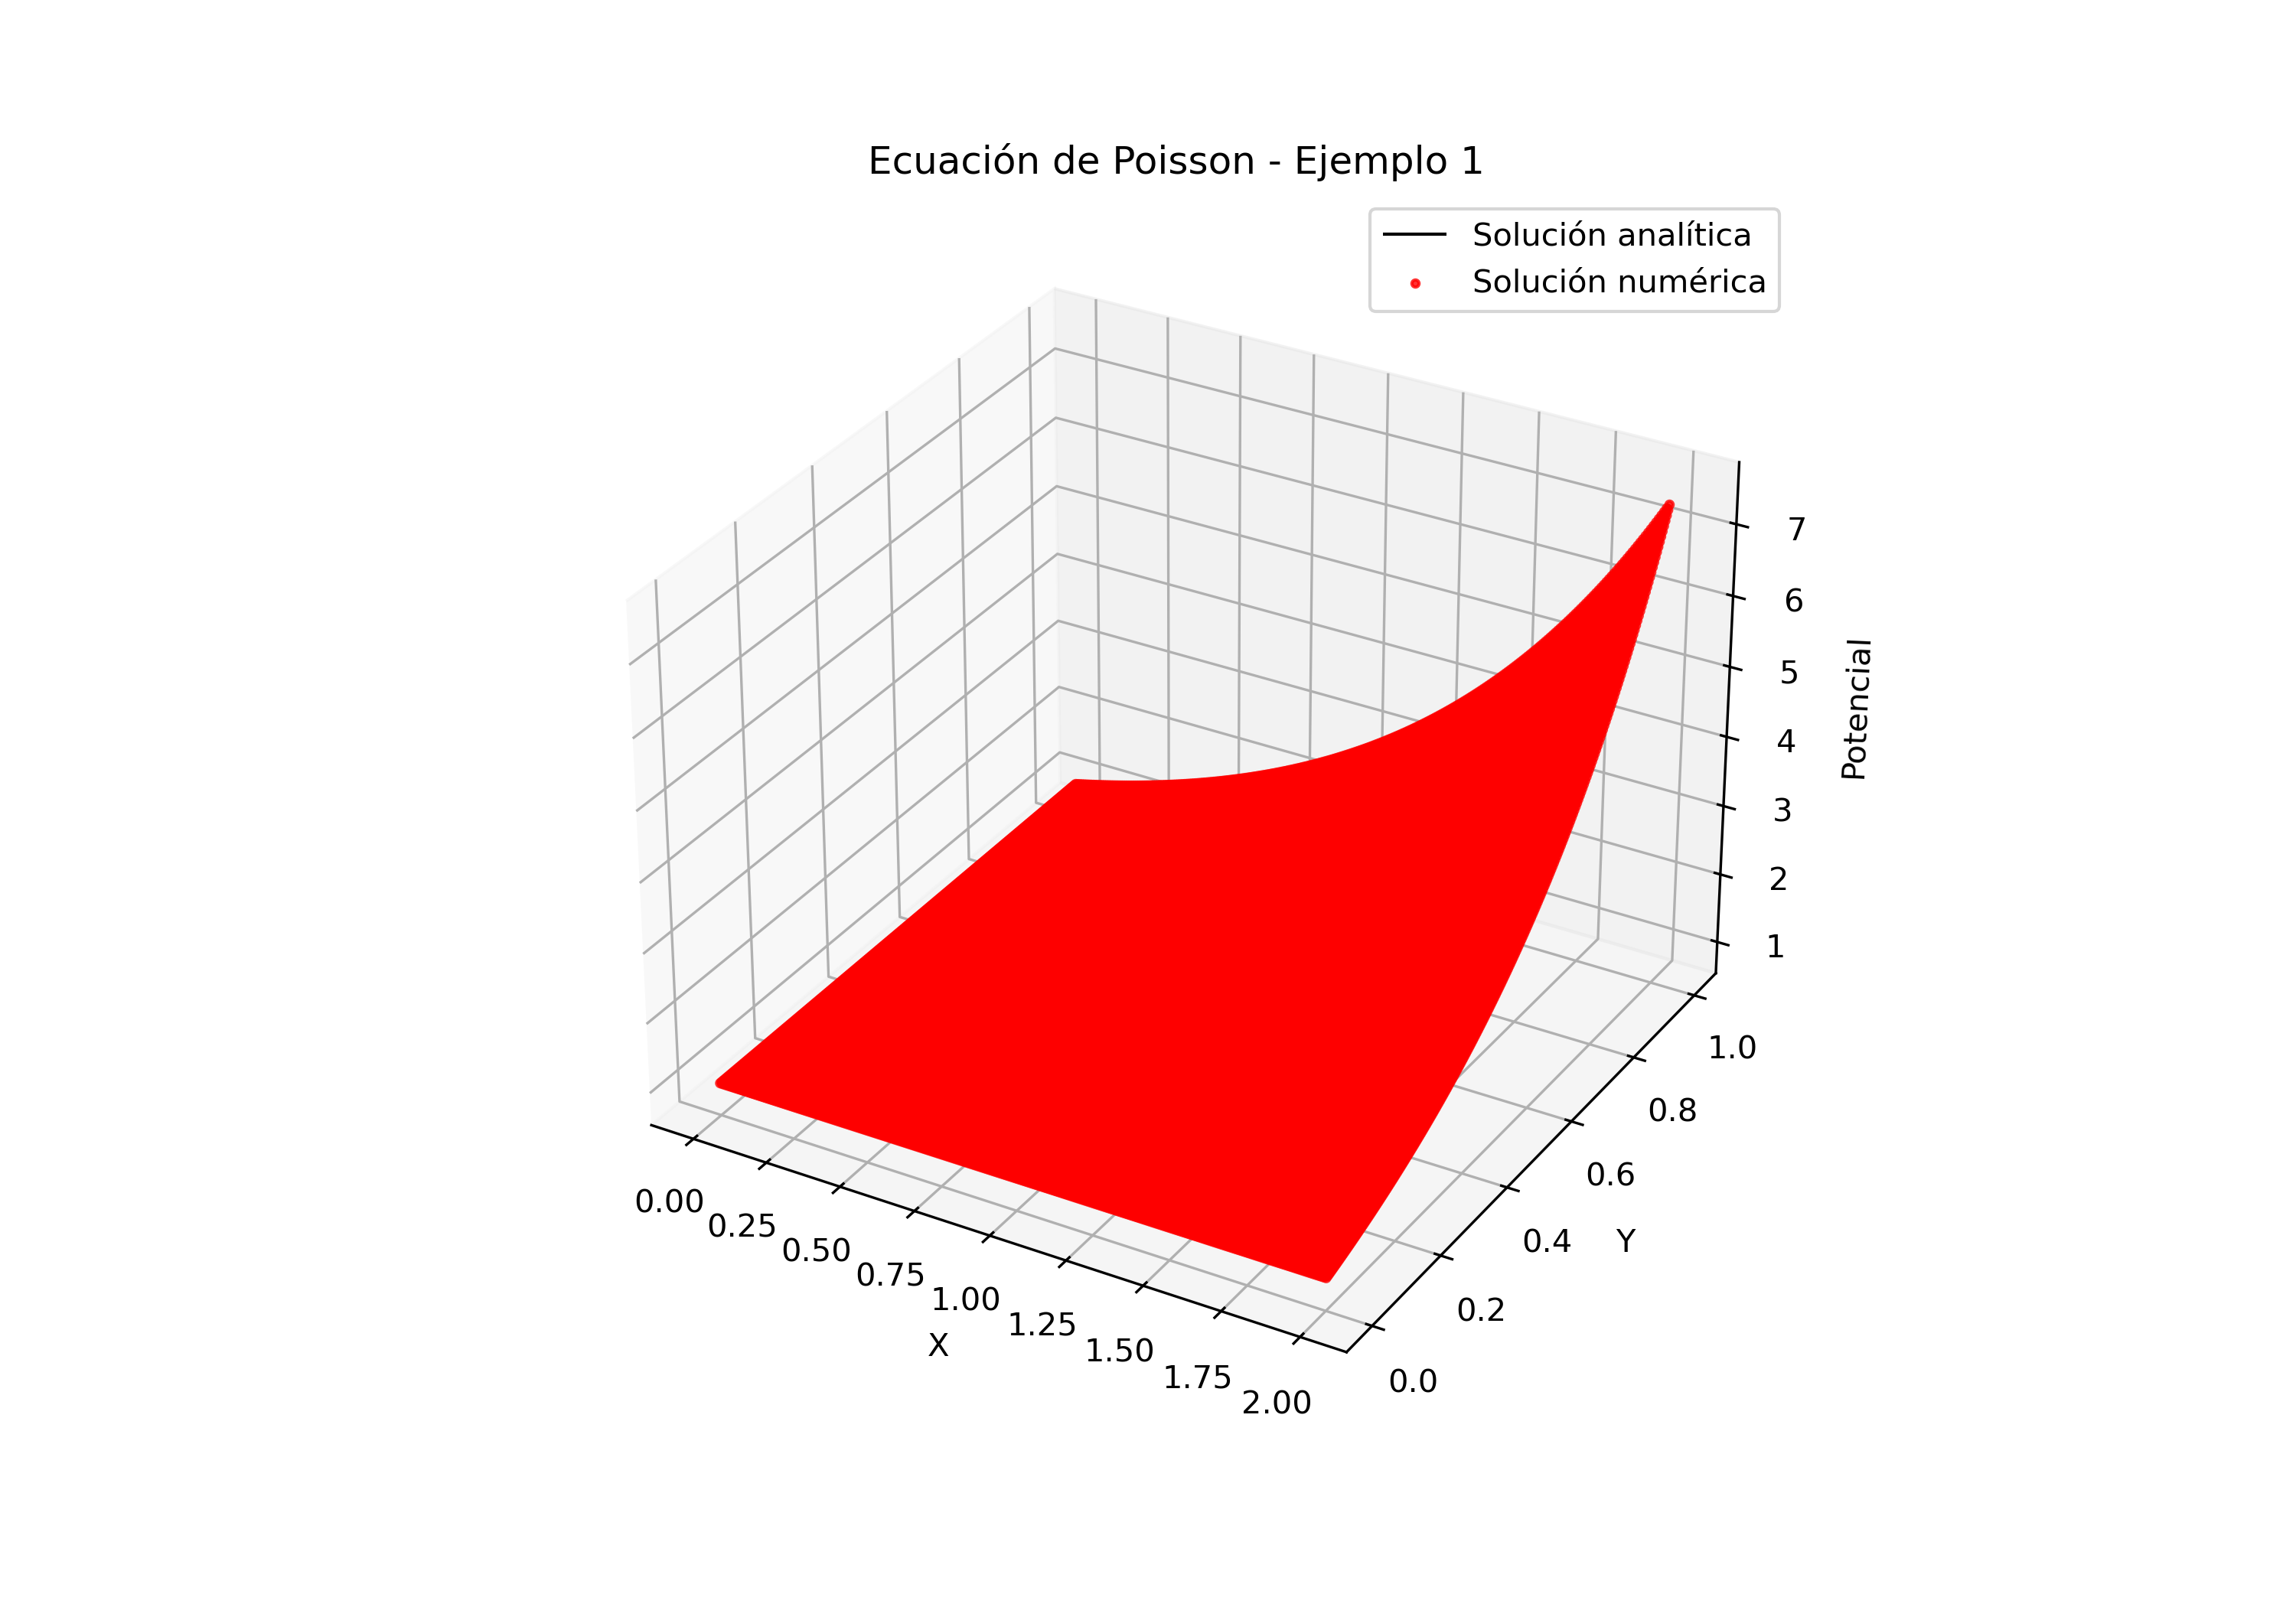
\includegraphics[width=0.8\textwidth]{imag/solucion_parallel_for_Ej1.png}
    \caption{Ejemplo 1 resuelto con \texttt{parallel for collapse}.}
\end{figure}
\begin{figure}[H]
    \centering
    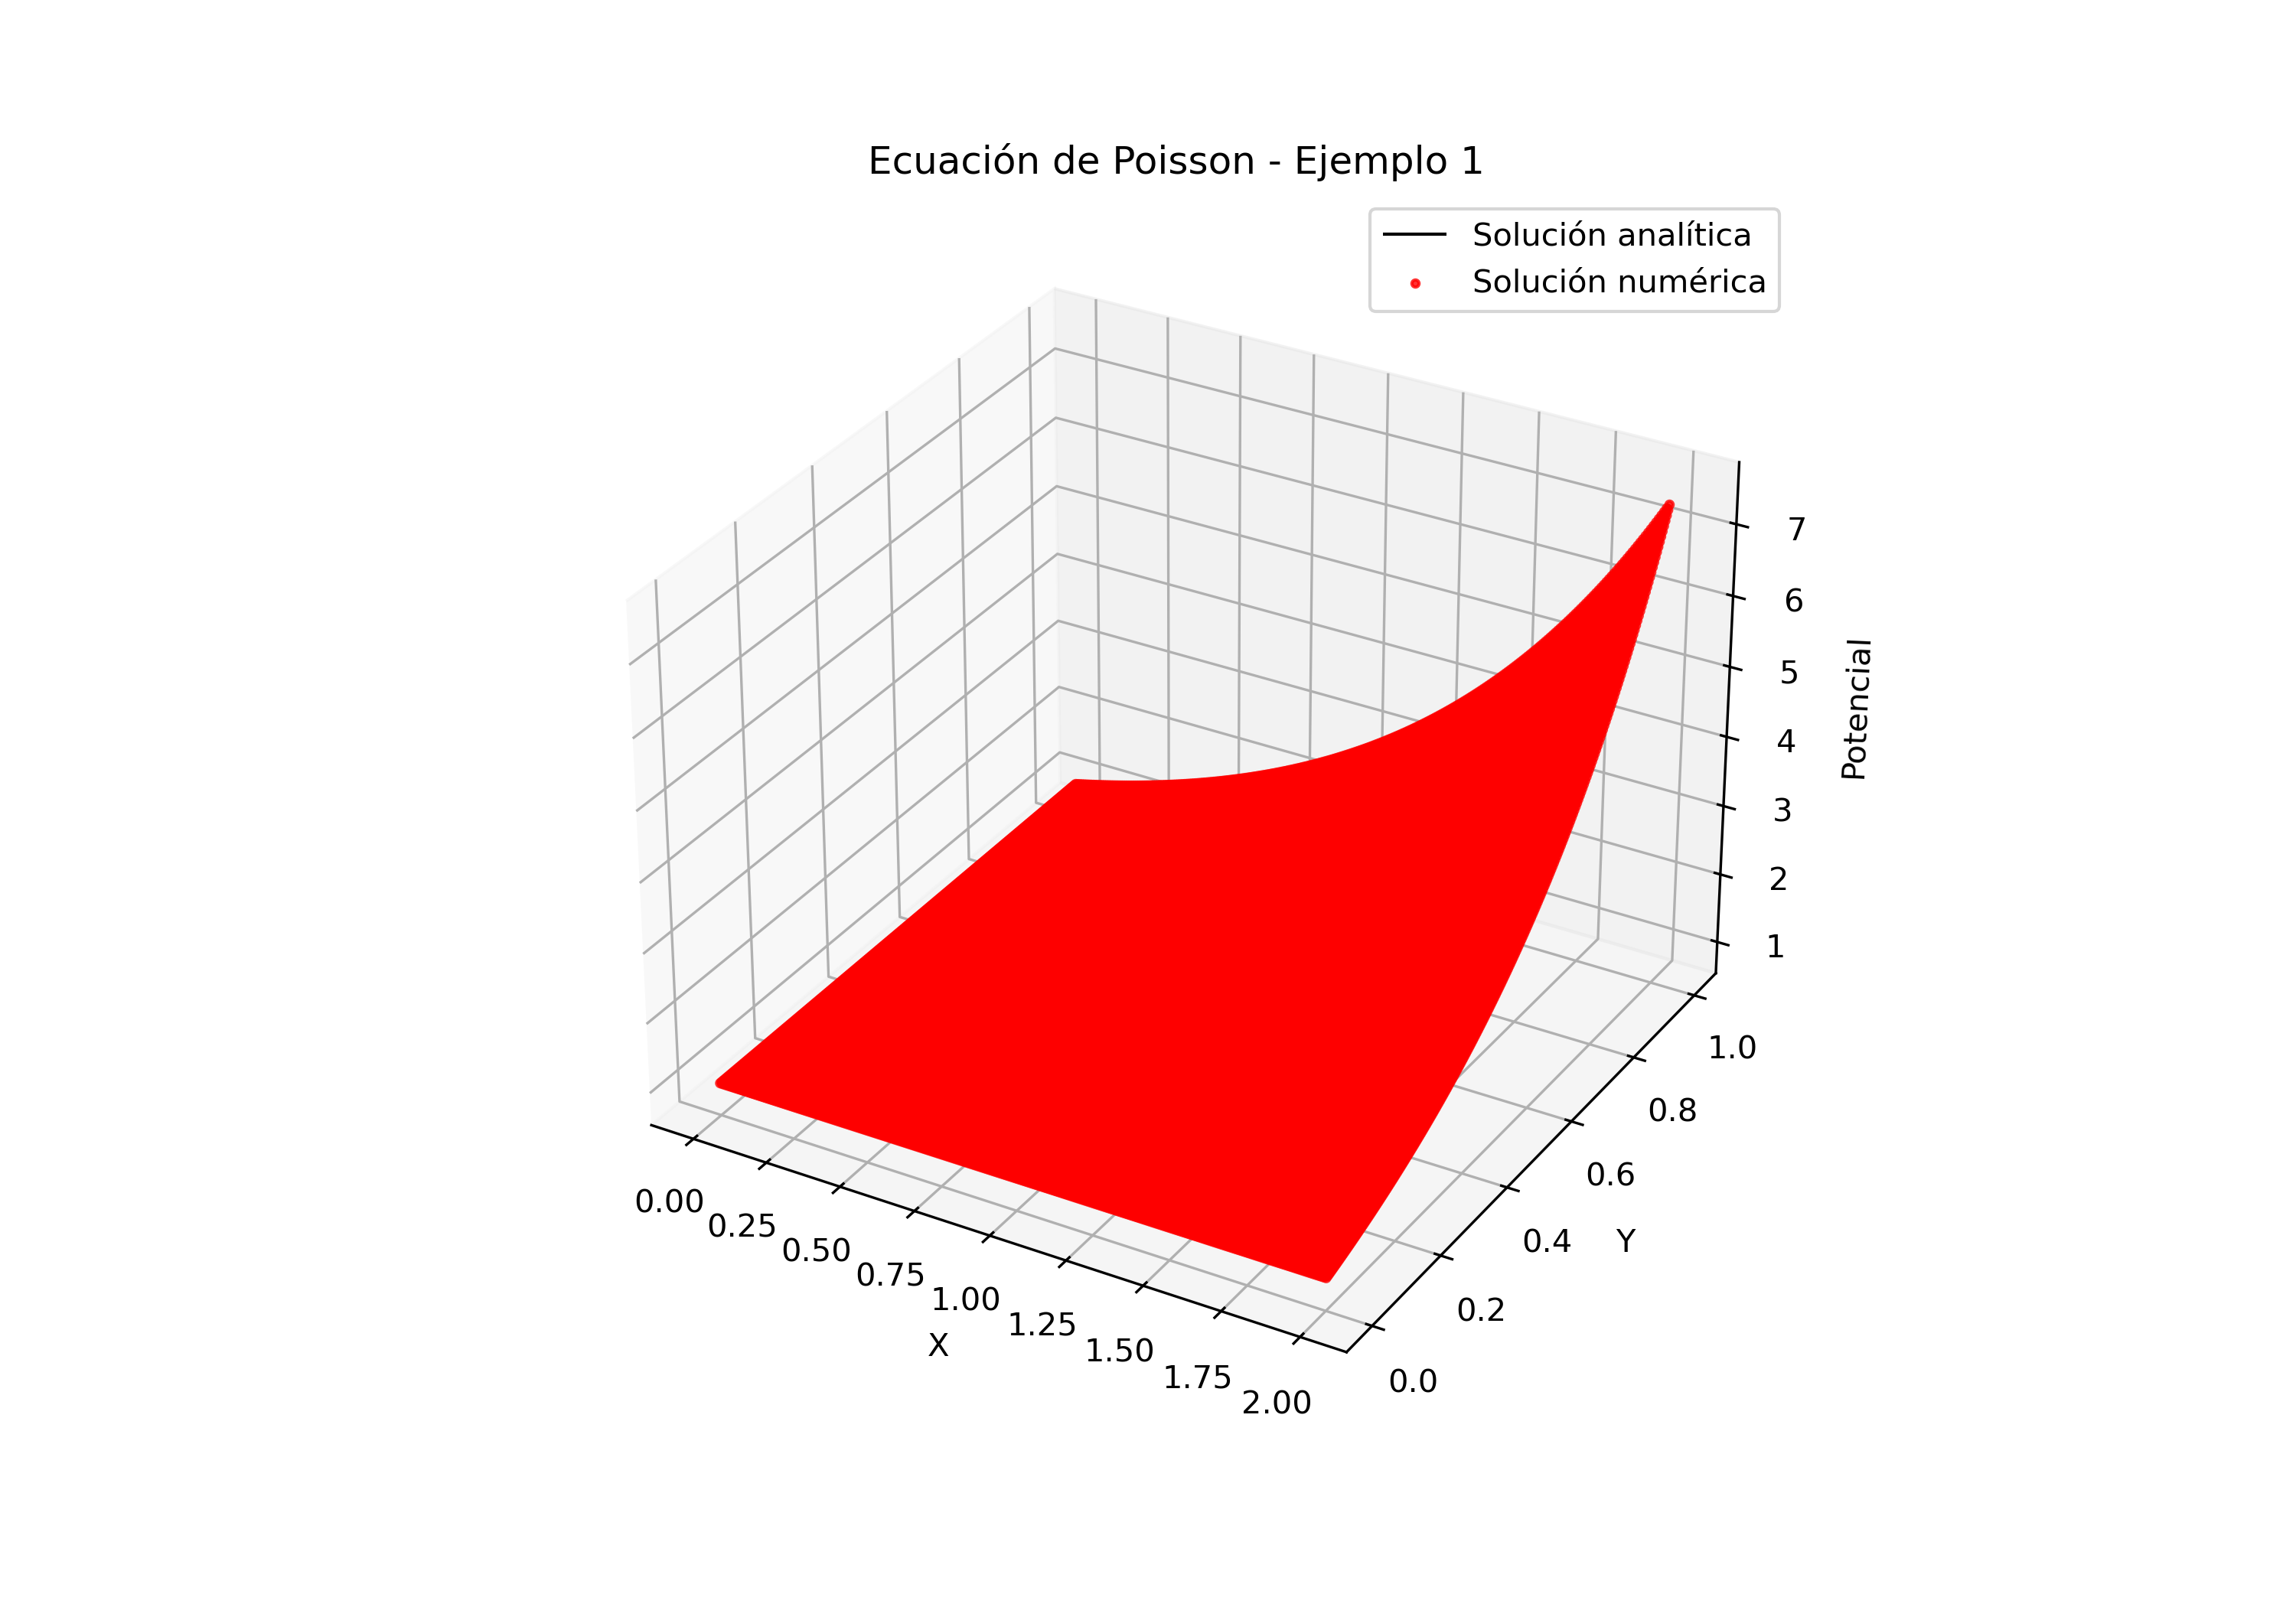
\includegraphics[width=0.8\textwidth]{imag/solucion_critical_Ej1.png}
    \caption{Ejemplo 1 resuelto con \texttt{critical}.}
\end{figure}
\begin{figure}[H]
    \centering
    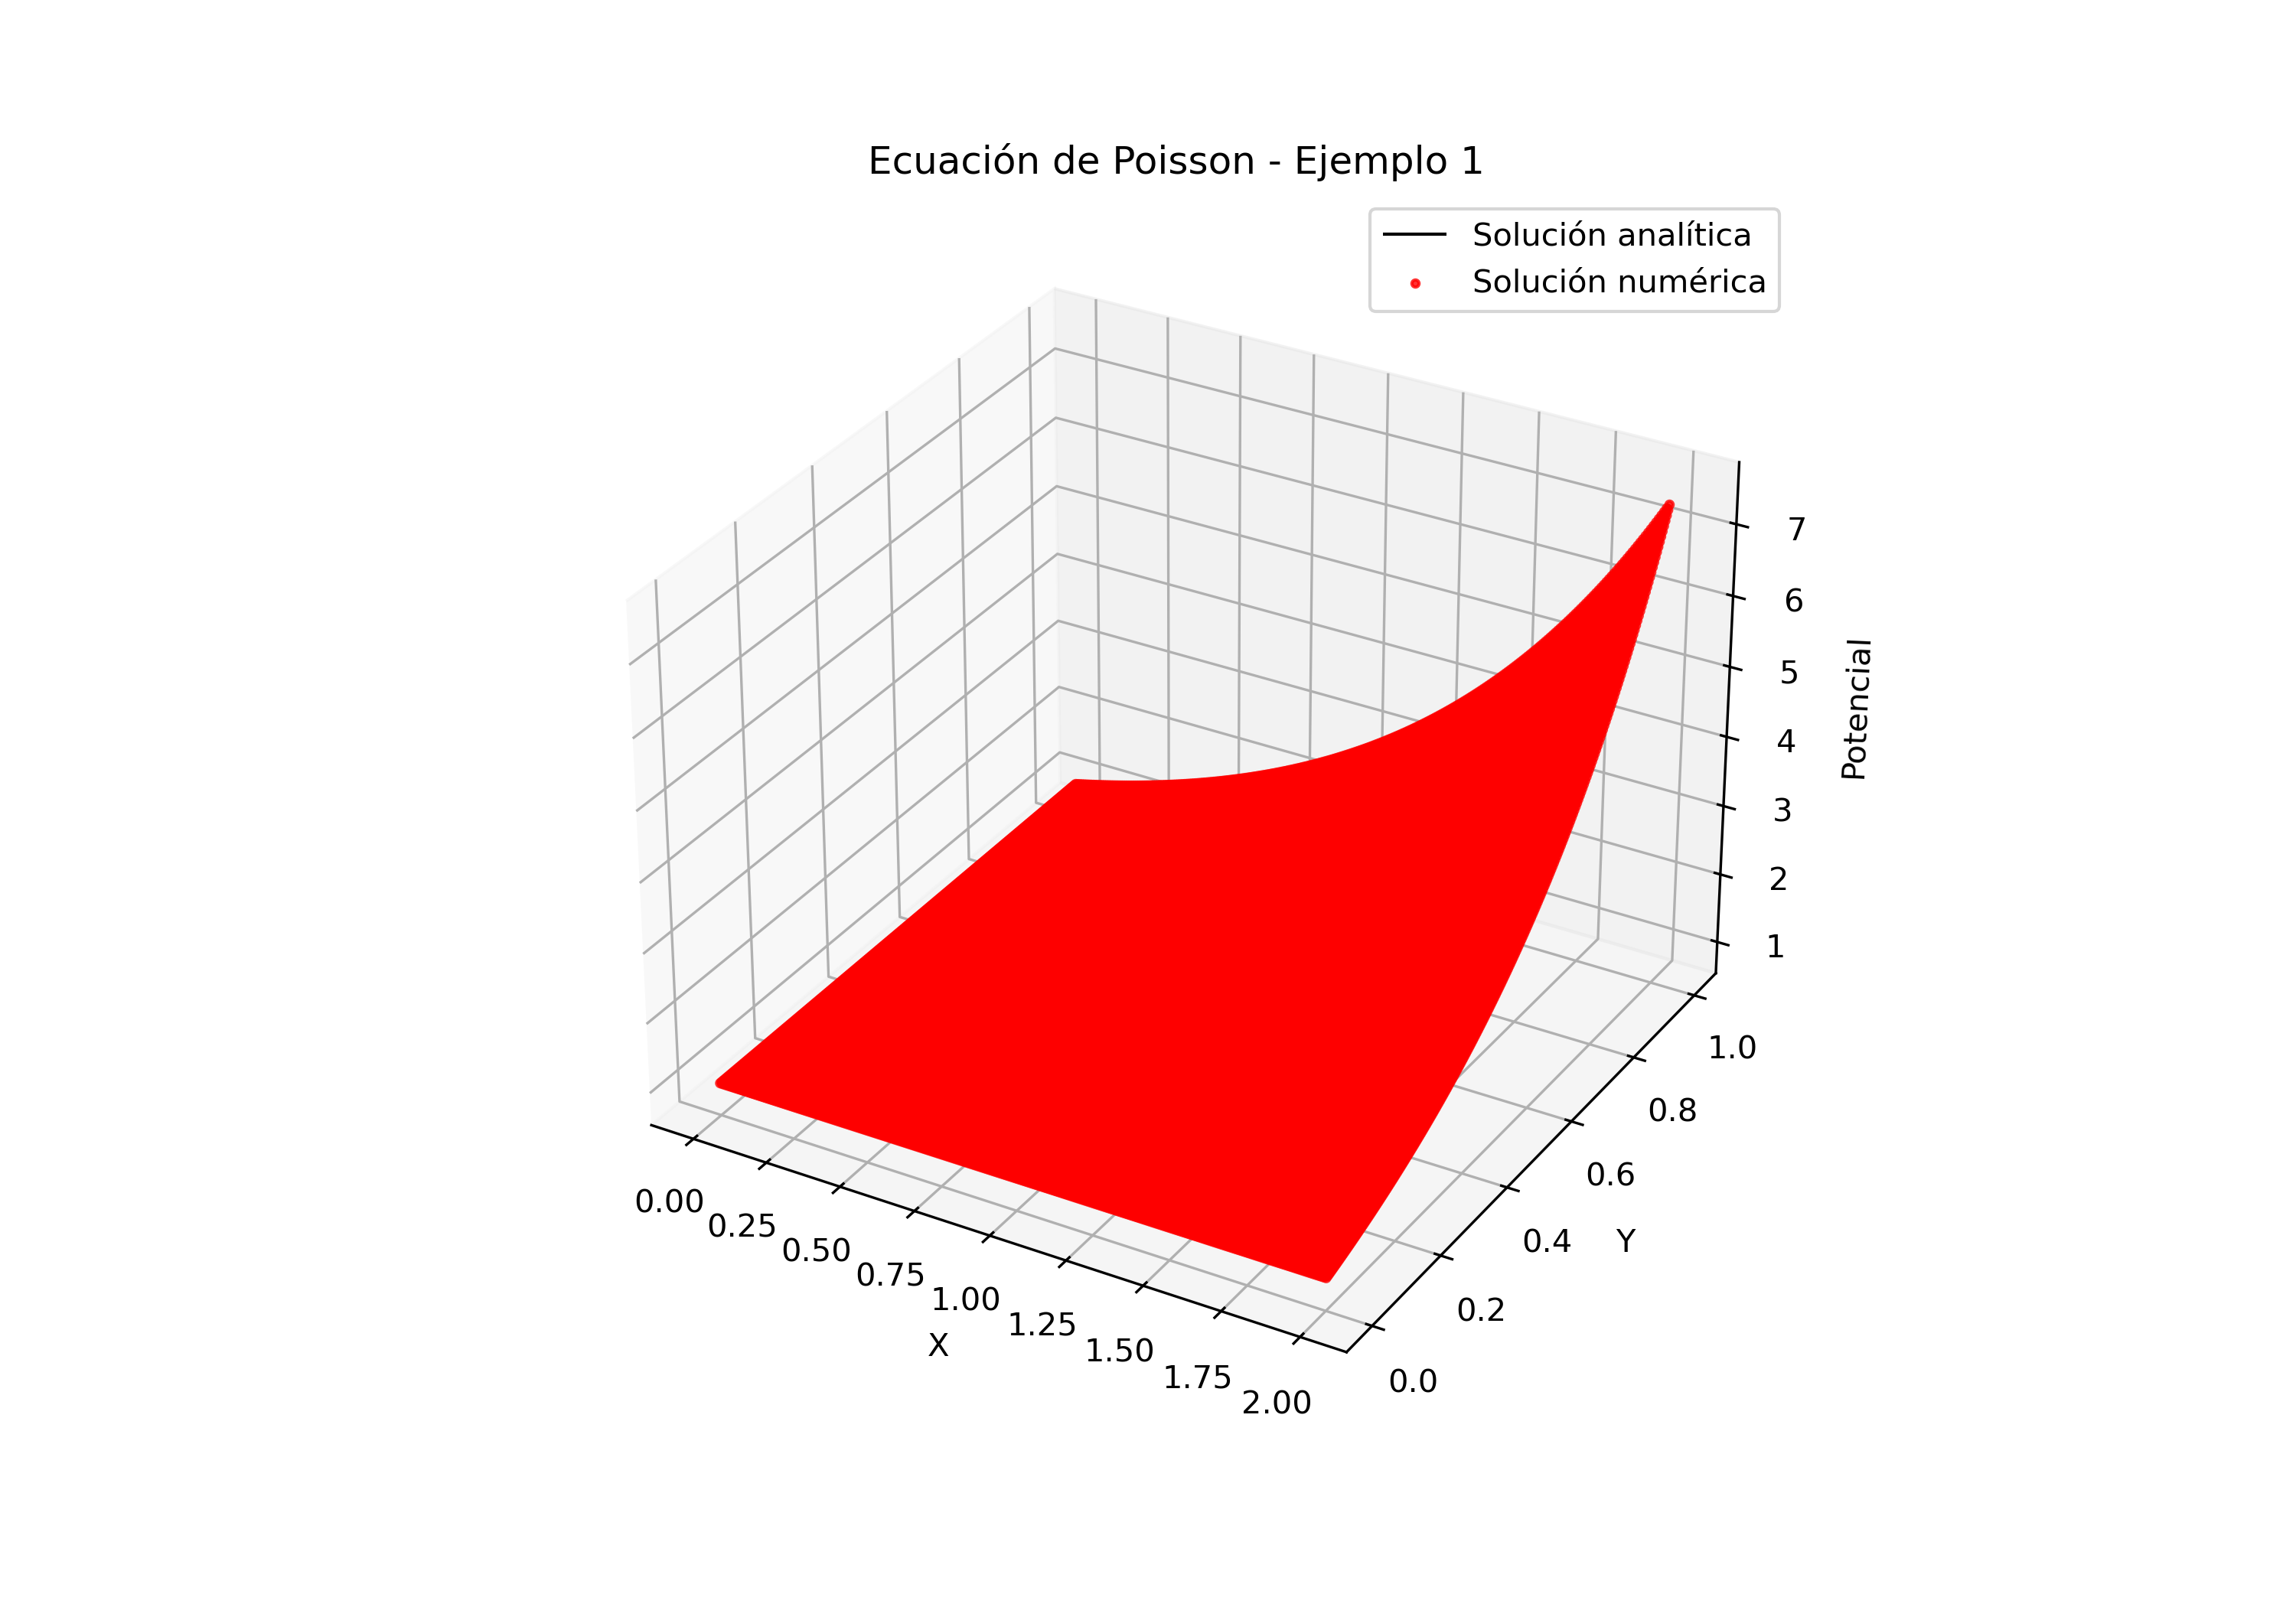
\includegraphics[width=0.8\textwidth]{imag/solucion_atomic_Ej1.png}
    \caption{Ejemplo 1 resuelto con \texttt{atomic}.}
\end{figure}
\begin{figure}[H]
    \centering
    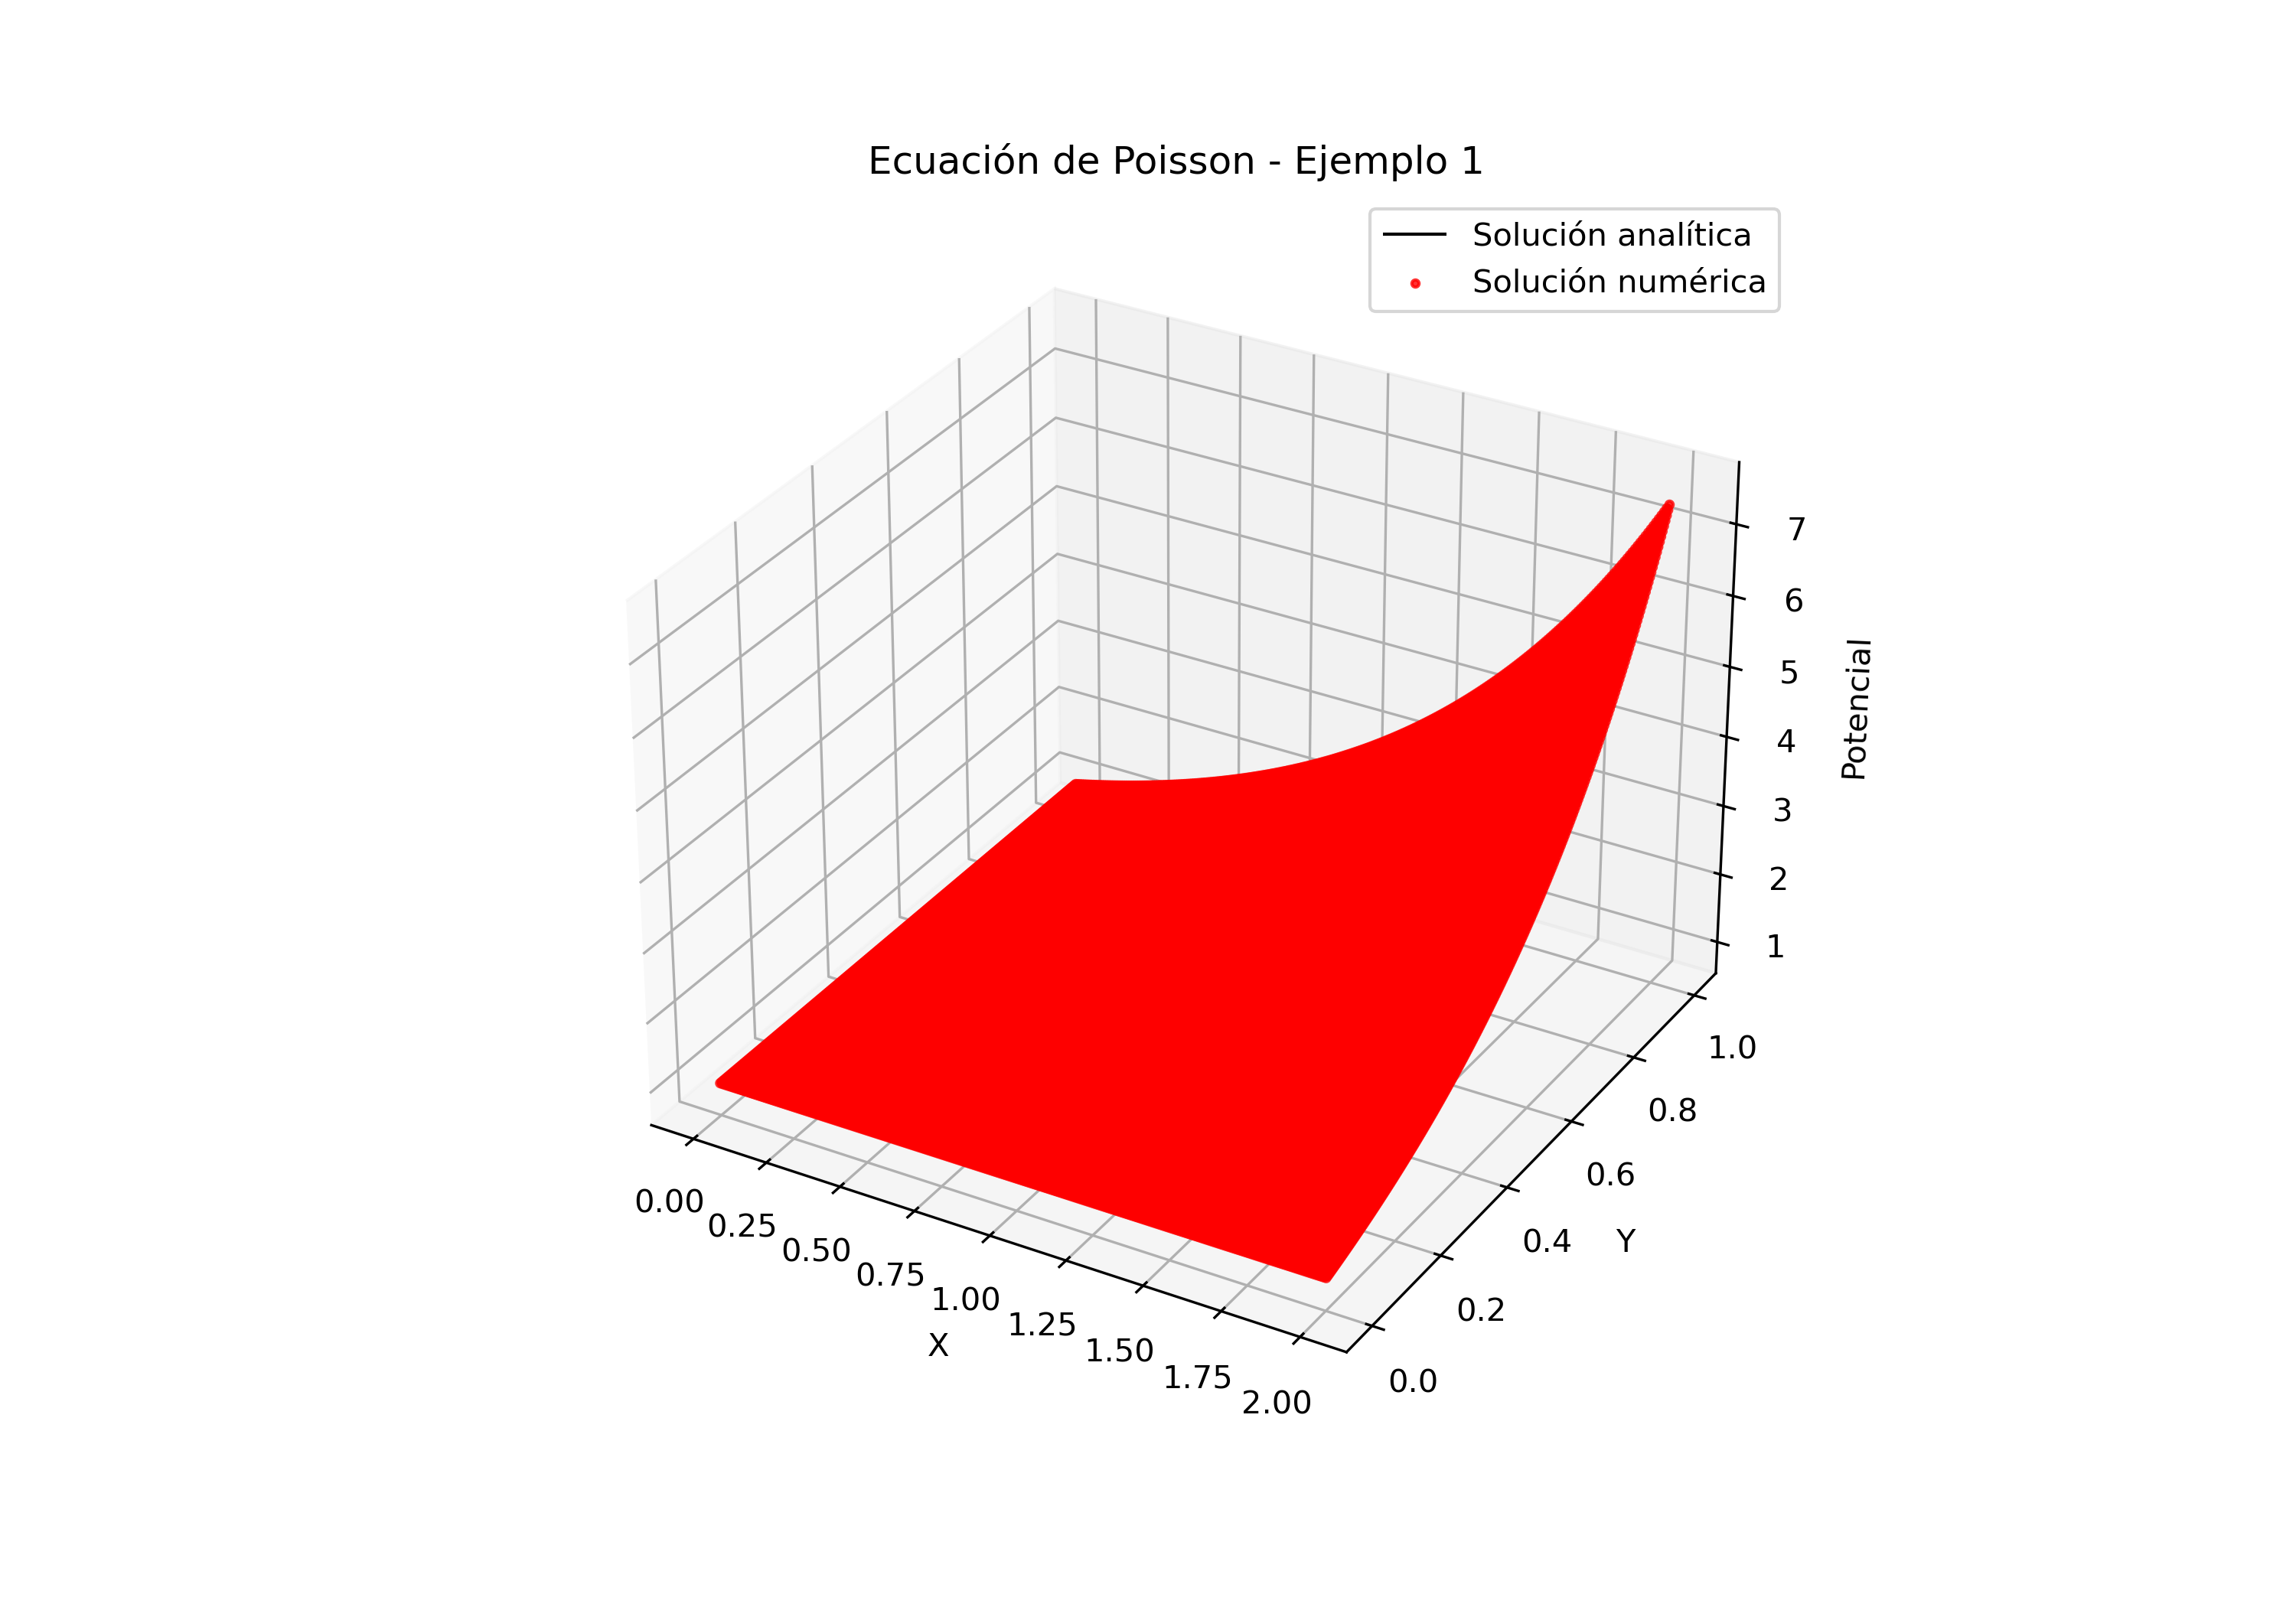
\includegraphics[width=0.8\textwidth]{imag/solucion_task_Ej1.png}
    \caption{Ejemplo 1 resuelto con \texttt{task}.}
\end{figure}

% === EJEMPLO 2 ===
\begin{figure}[H]
    \centering
    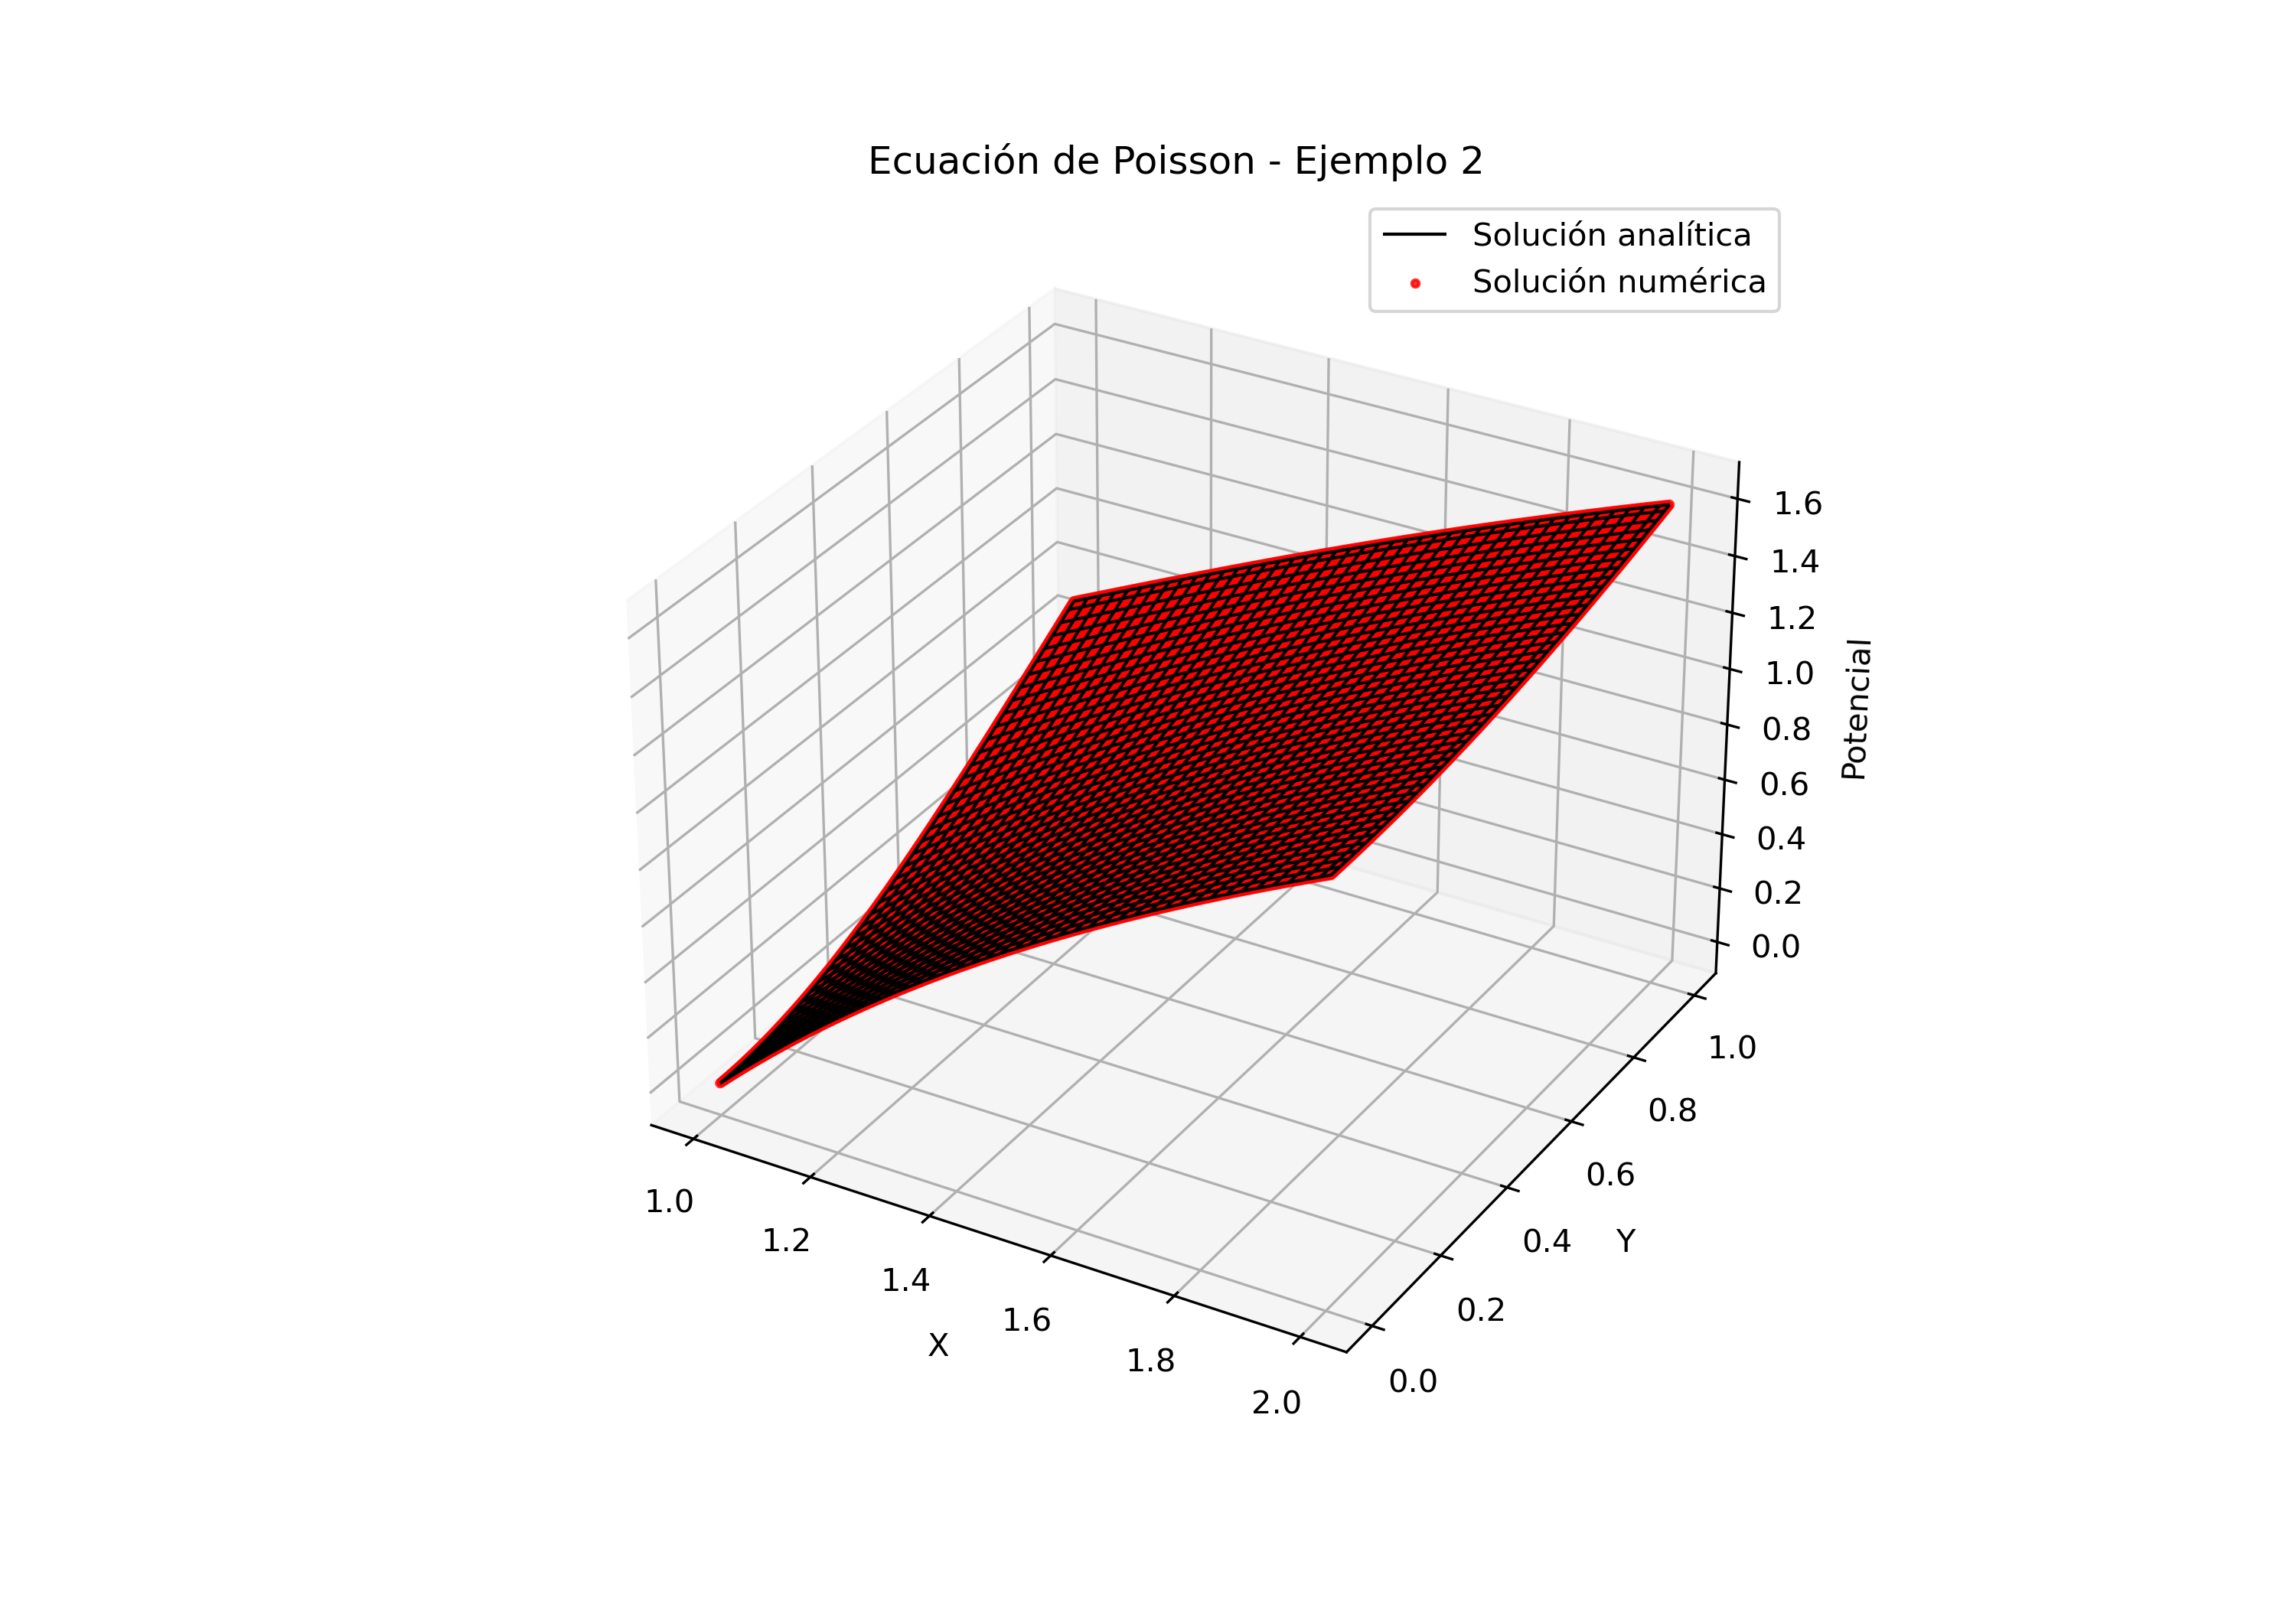
\includegraphics[width=0.8\textwidth]{imag/solucion_serial_Ej2.png}
    \caption{Ejemplo 2 resuelto con método secuencial.}
\end{figure}
\begin{figure}[H]
    \centering
    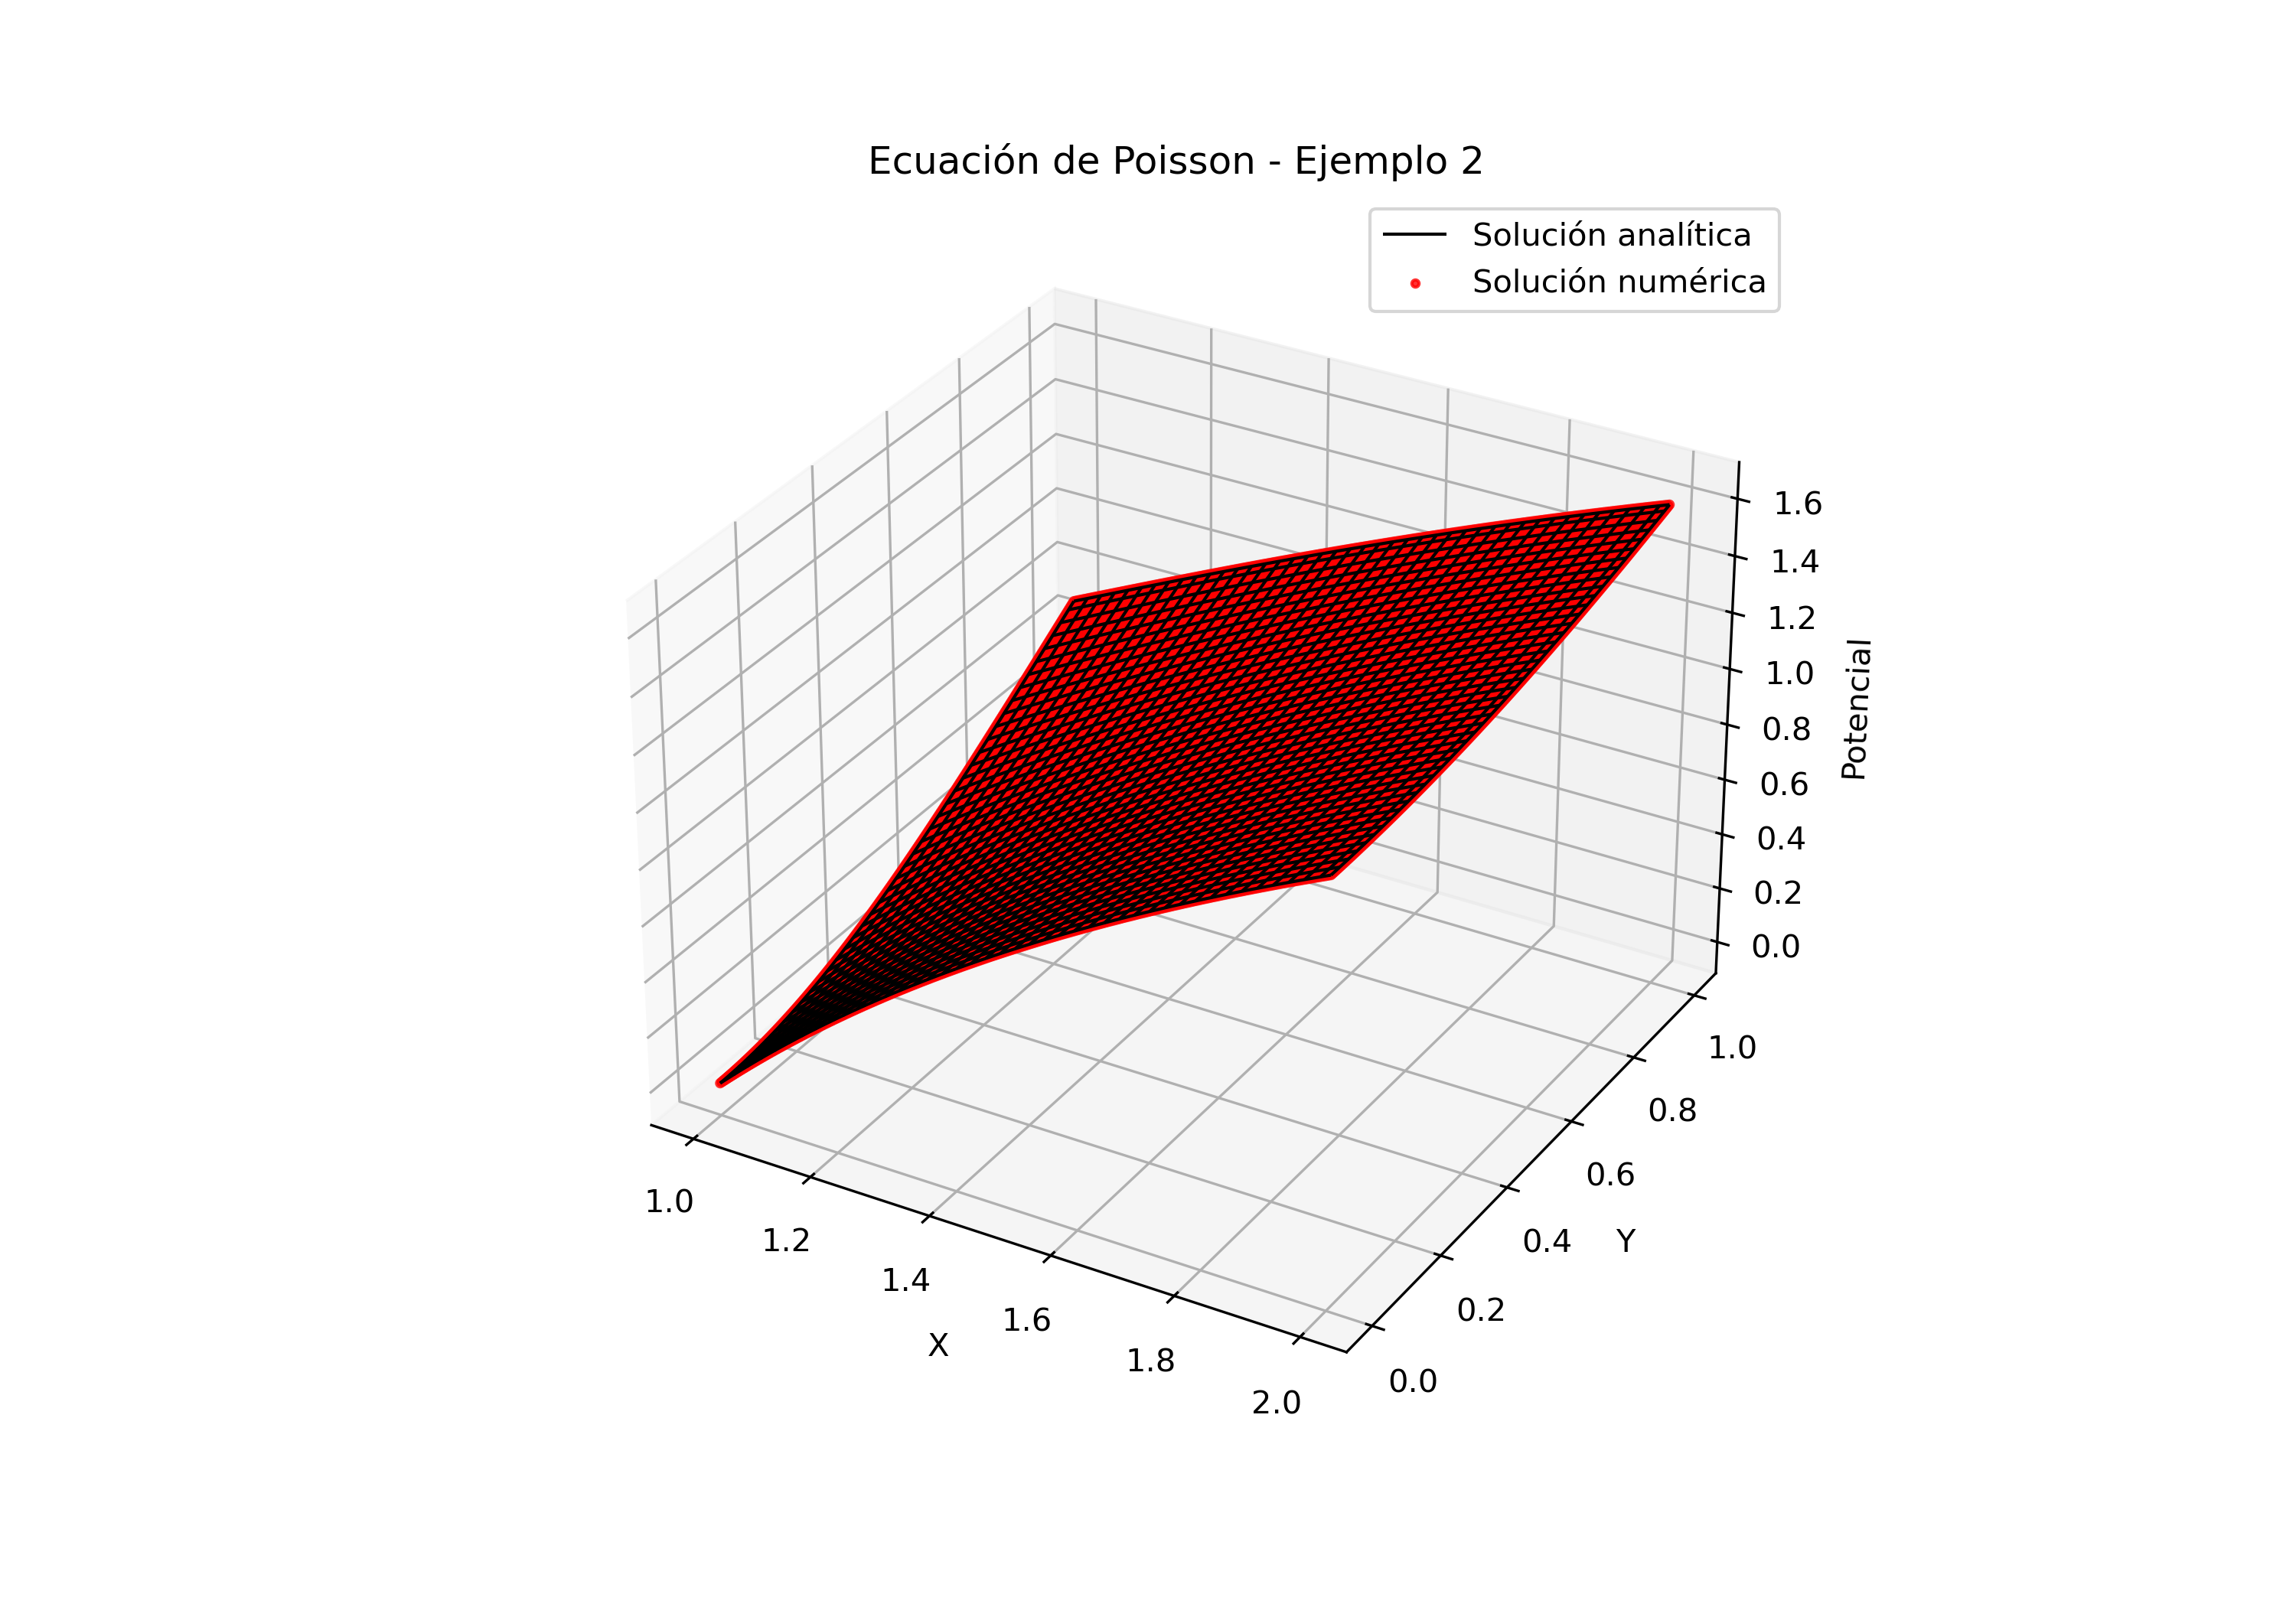
\includegraphics[width=0.8\textwidth]{imag/solucion_parallel_for_Ej2.png}
    \caption{Ejemplo 2 resuelto con \texttt{parallel for collapse}.}
\end{figure}
\begin{figure}[H]
    \centering
    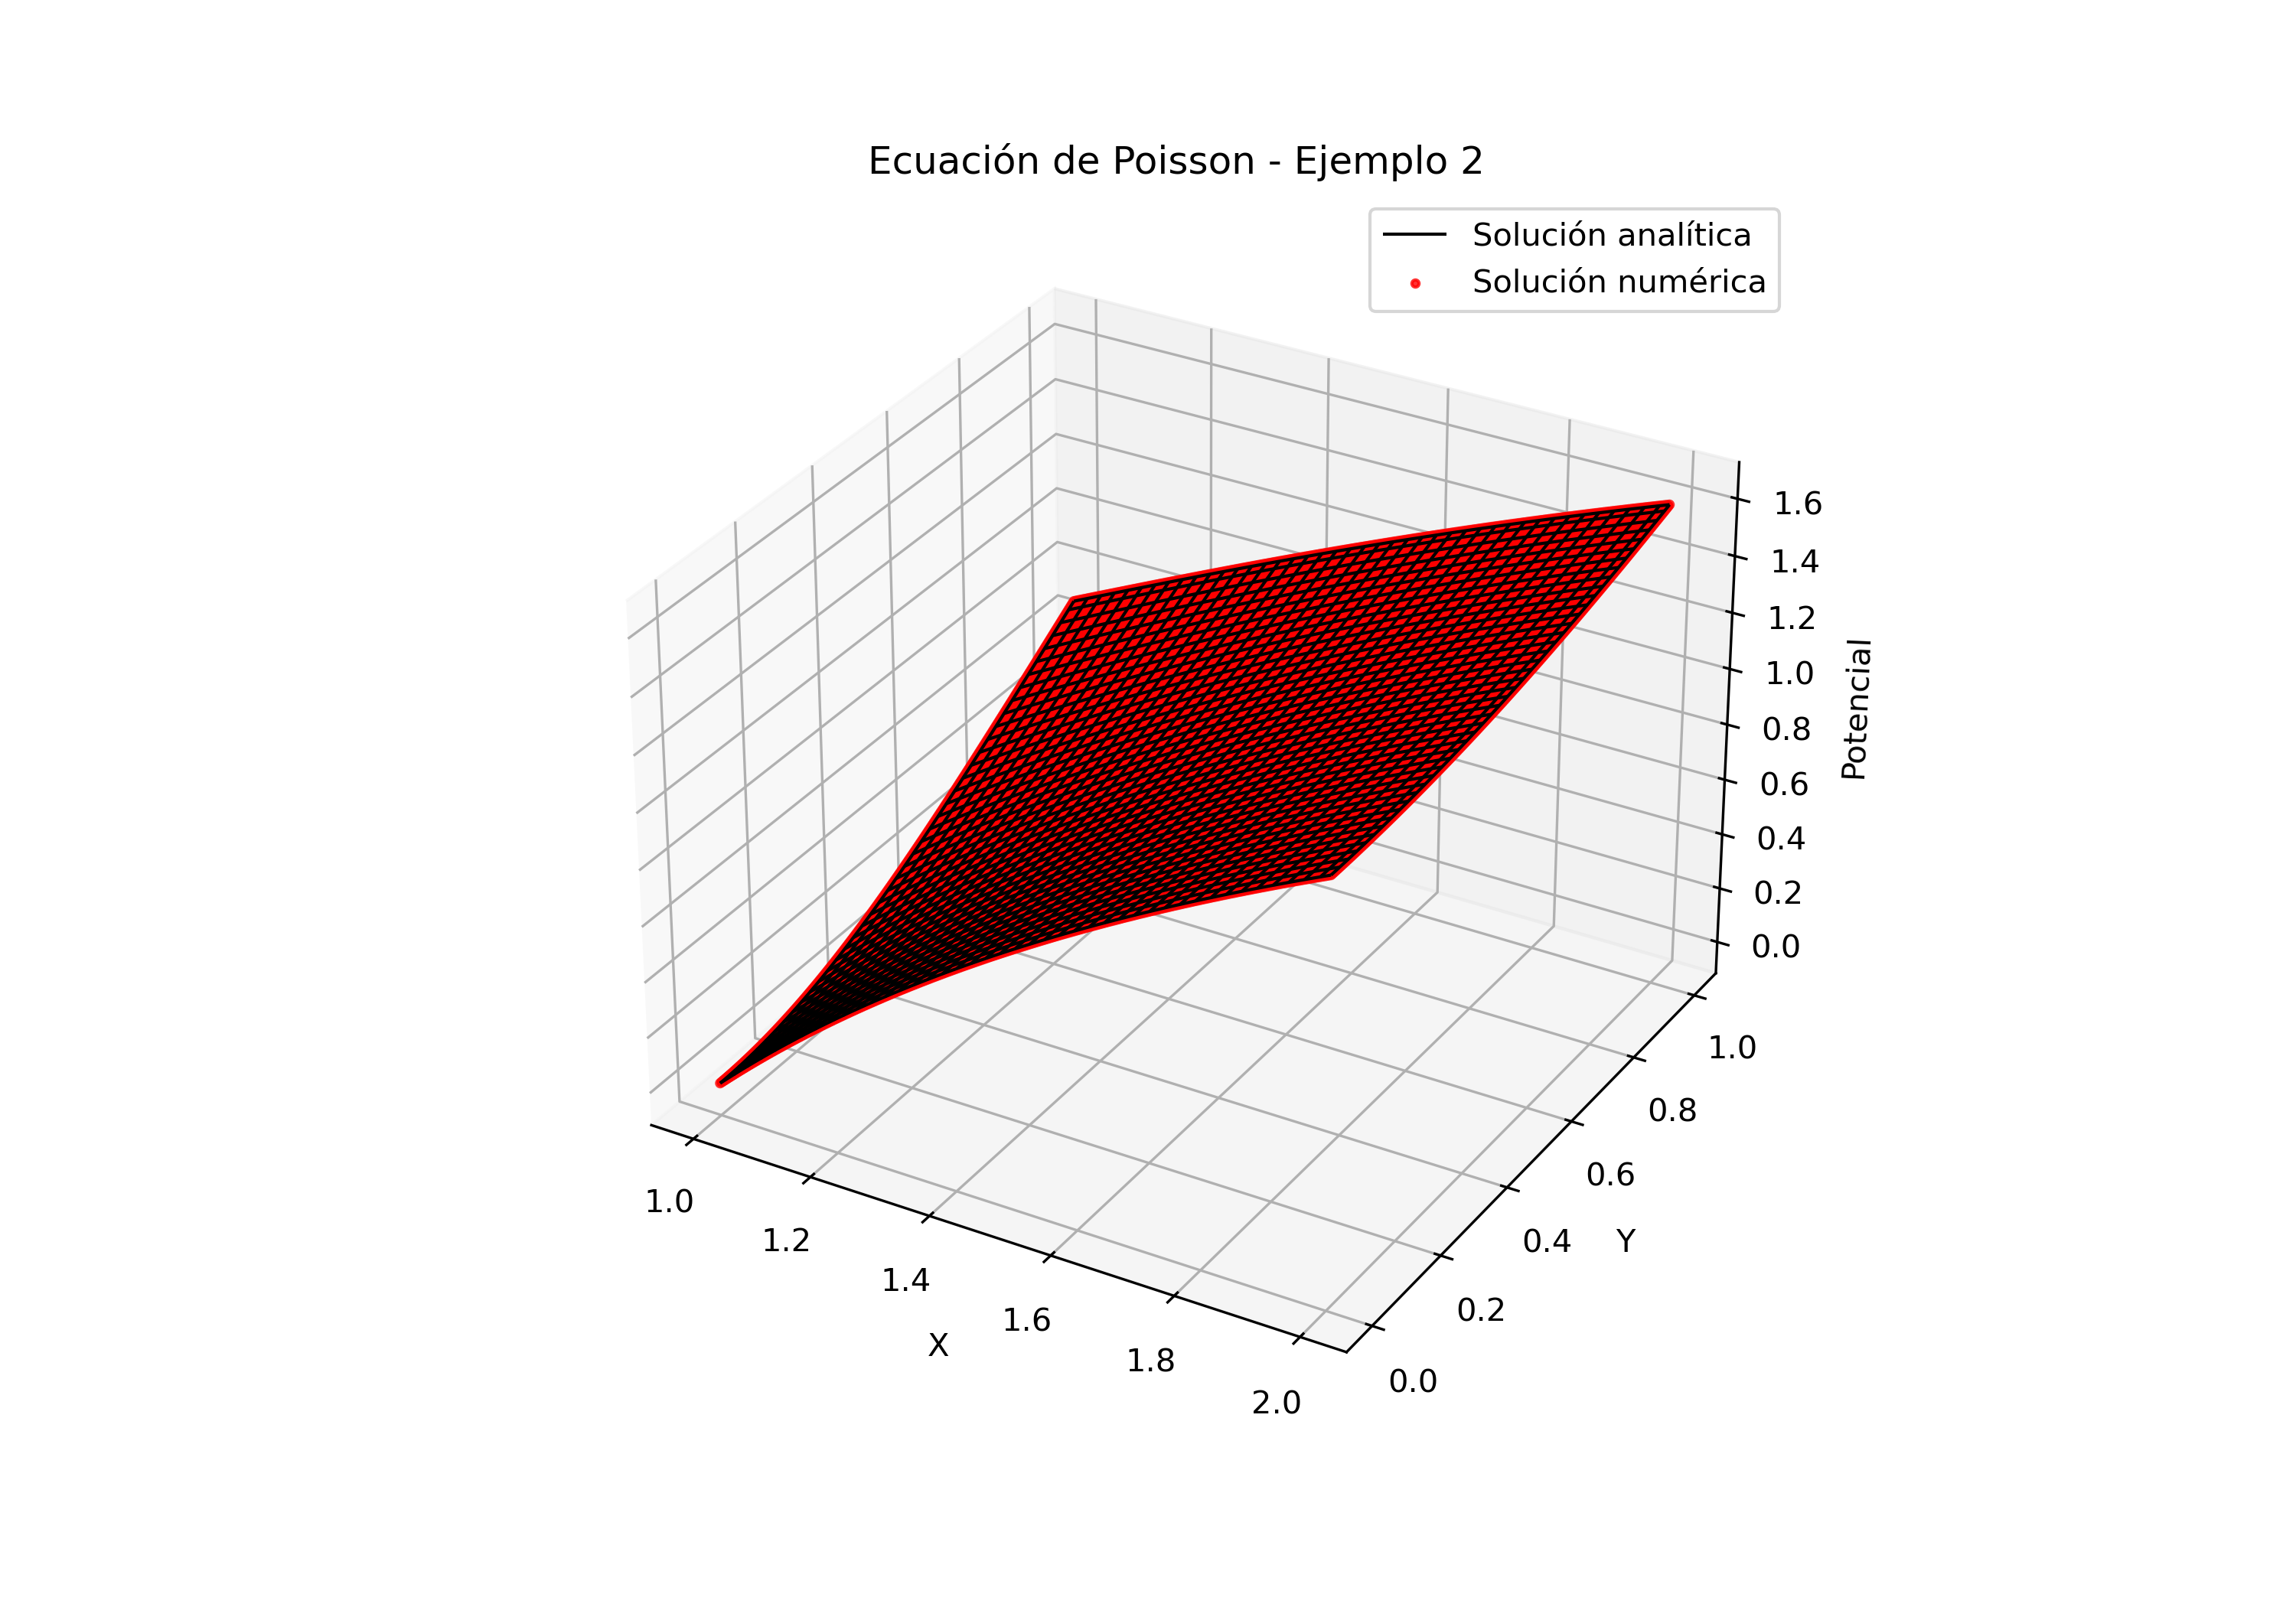
\includegraphics[width=0.8\textwidth]{imag/solucion_critical_Ej2.png}
    \caption{Ejemplo 2 resuelto con \texttt{critical}.}
\end{figure}
\begin{figure}[H]
    \centering
    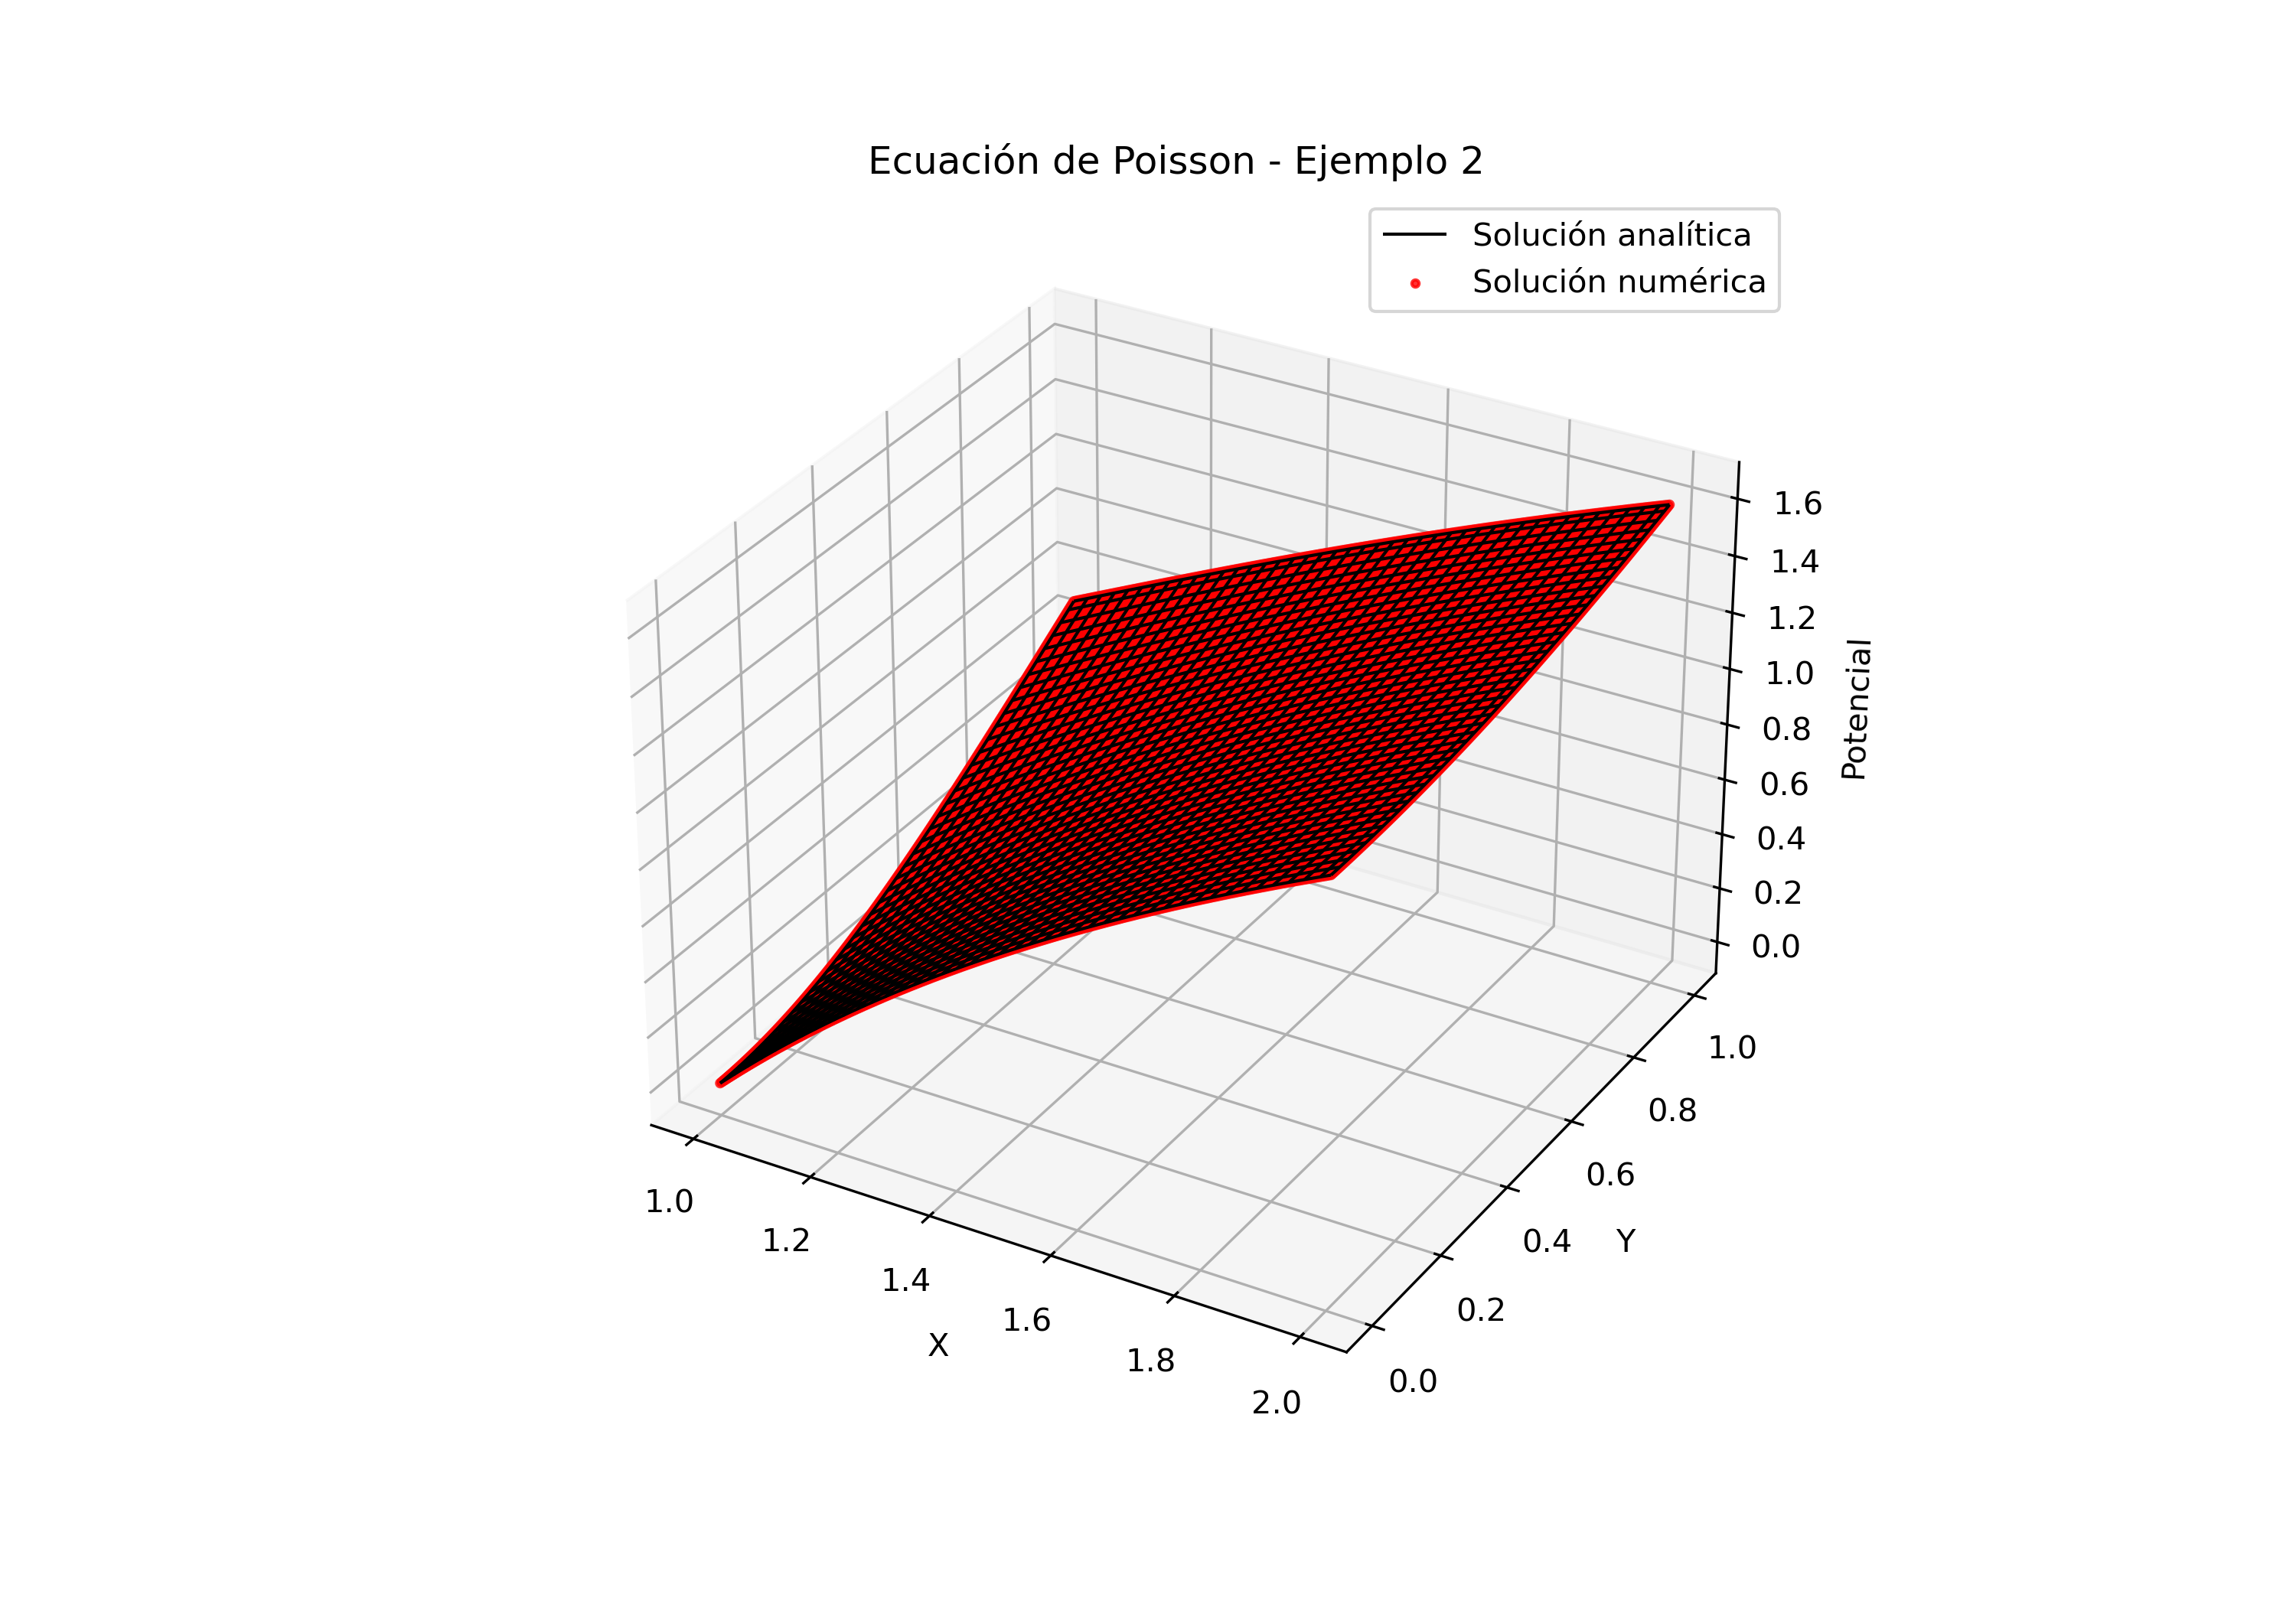
\includegraphics[width=0.8\textwidth]{imag/solucion_atomic_Ej2.png}
    \caption{Ejemplo 2 resuelto con \texttt{atomic}.}
\end{figure}
\begin{figure}[H]
    \centering
    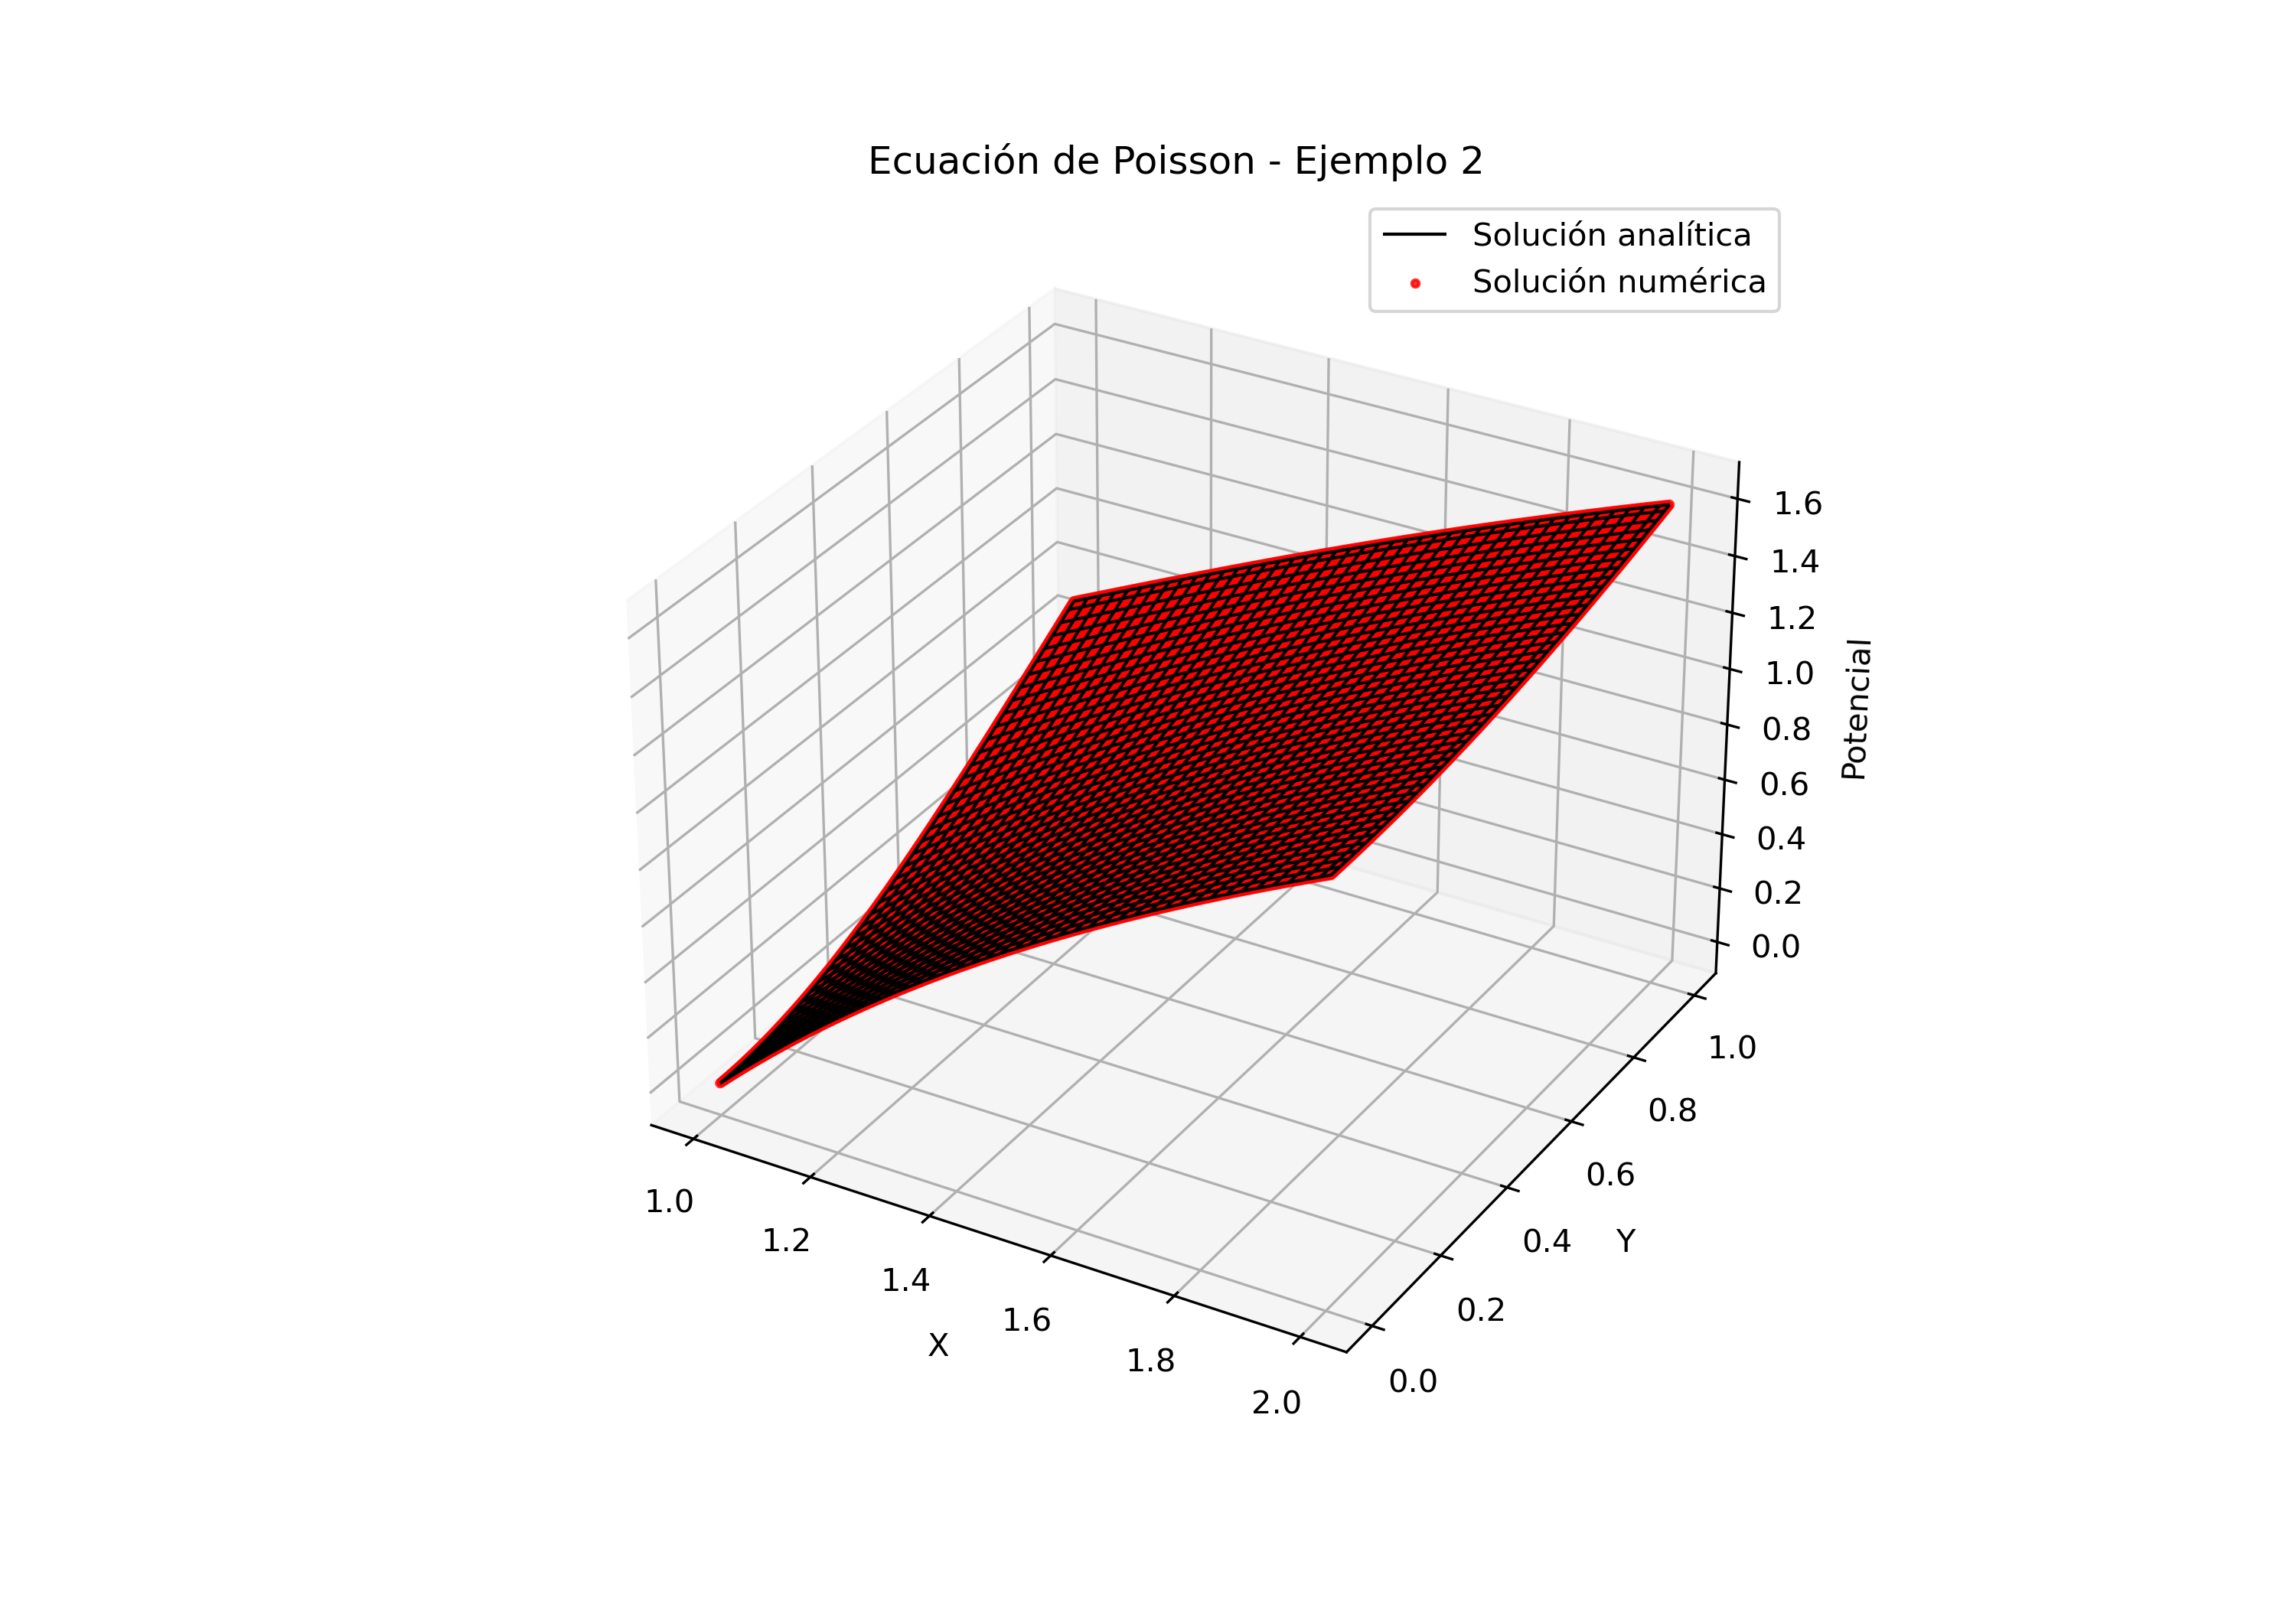
\includegraphics[width=0.8\textwidth]{imag/solucion_task_Ej2.png}
    \caption{Ejemplo 2 resuelto con \texttt{task}.}
\end{figure}

% === EJEMPLO 3 ===
\begin{figure}[H]
    \centering
    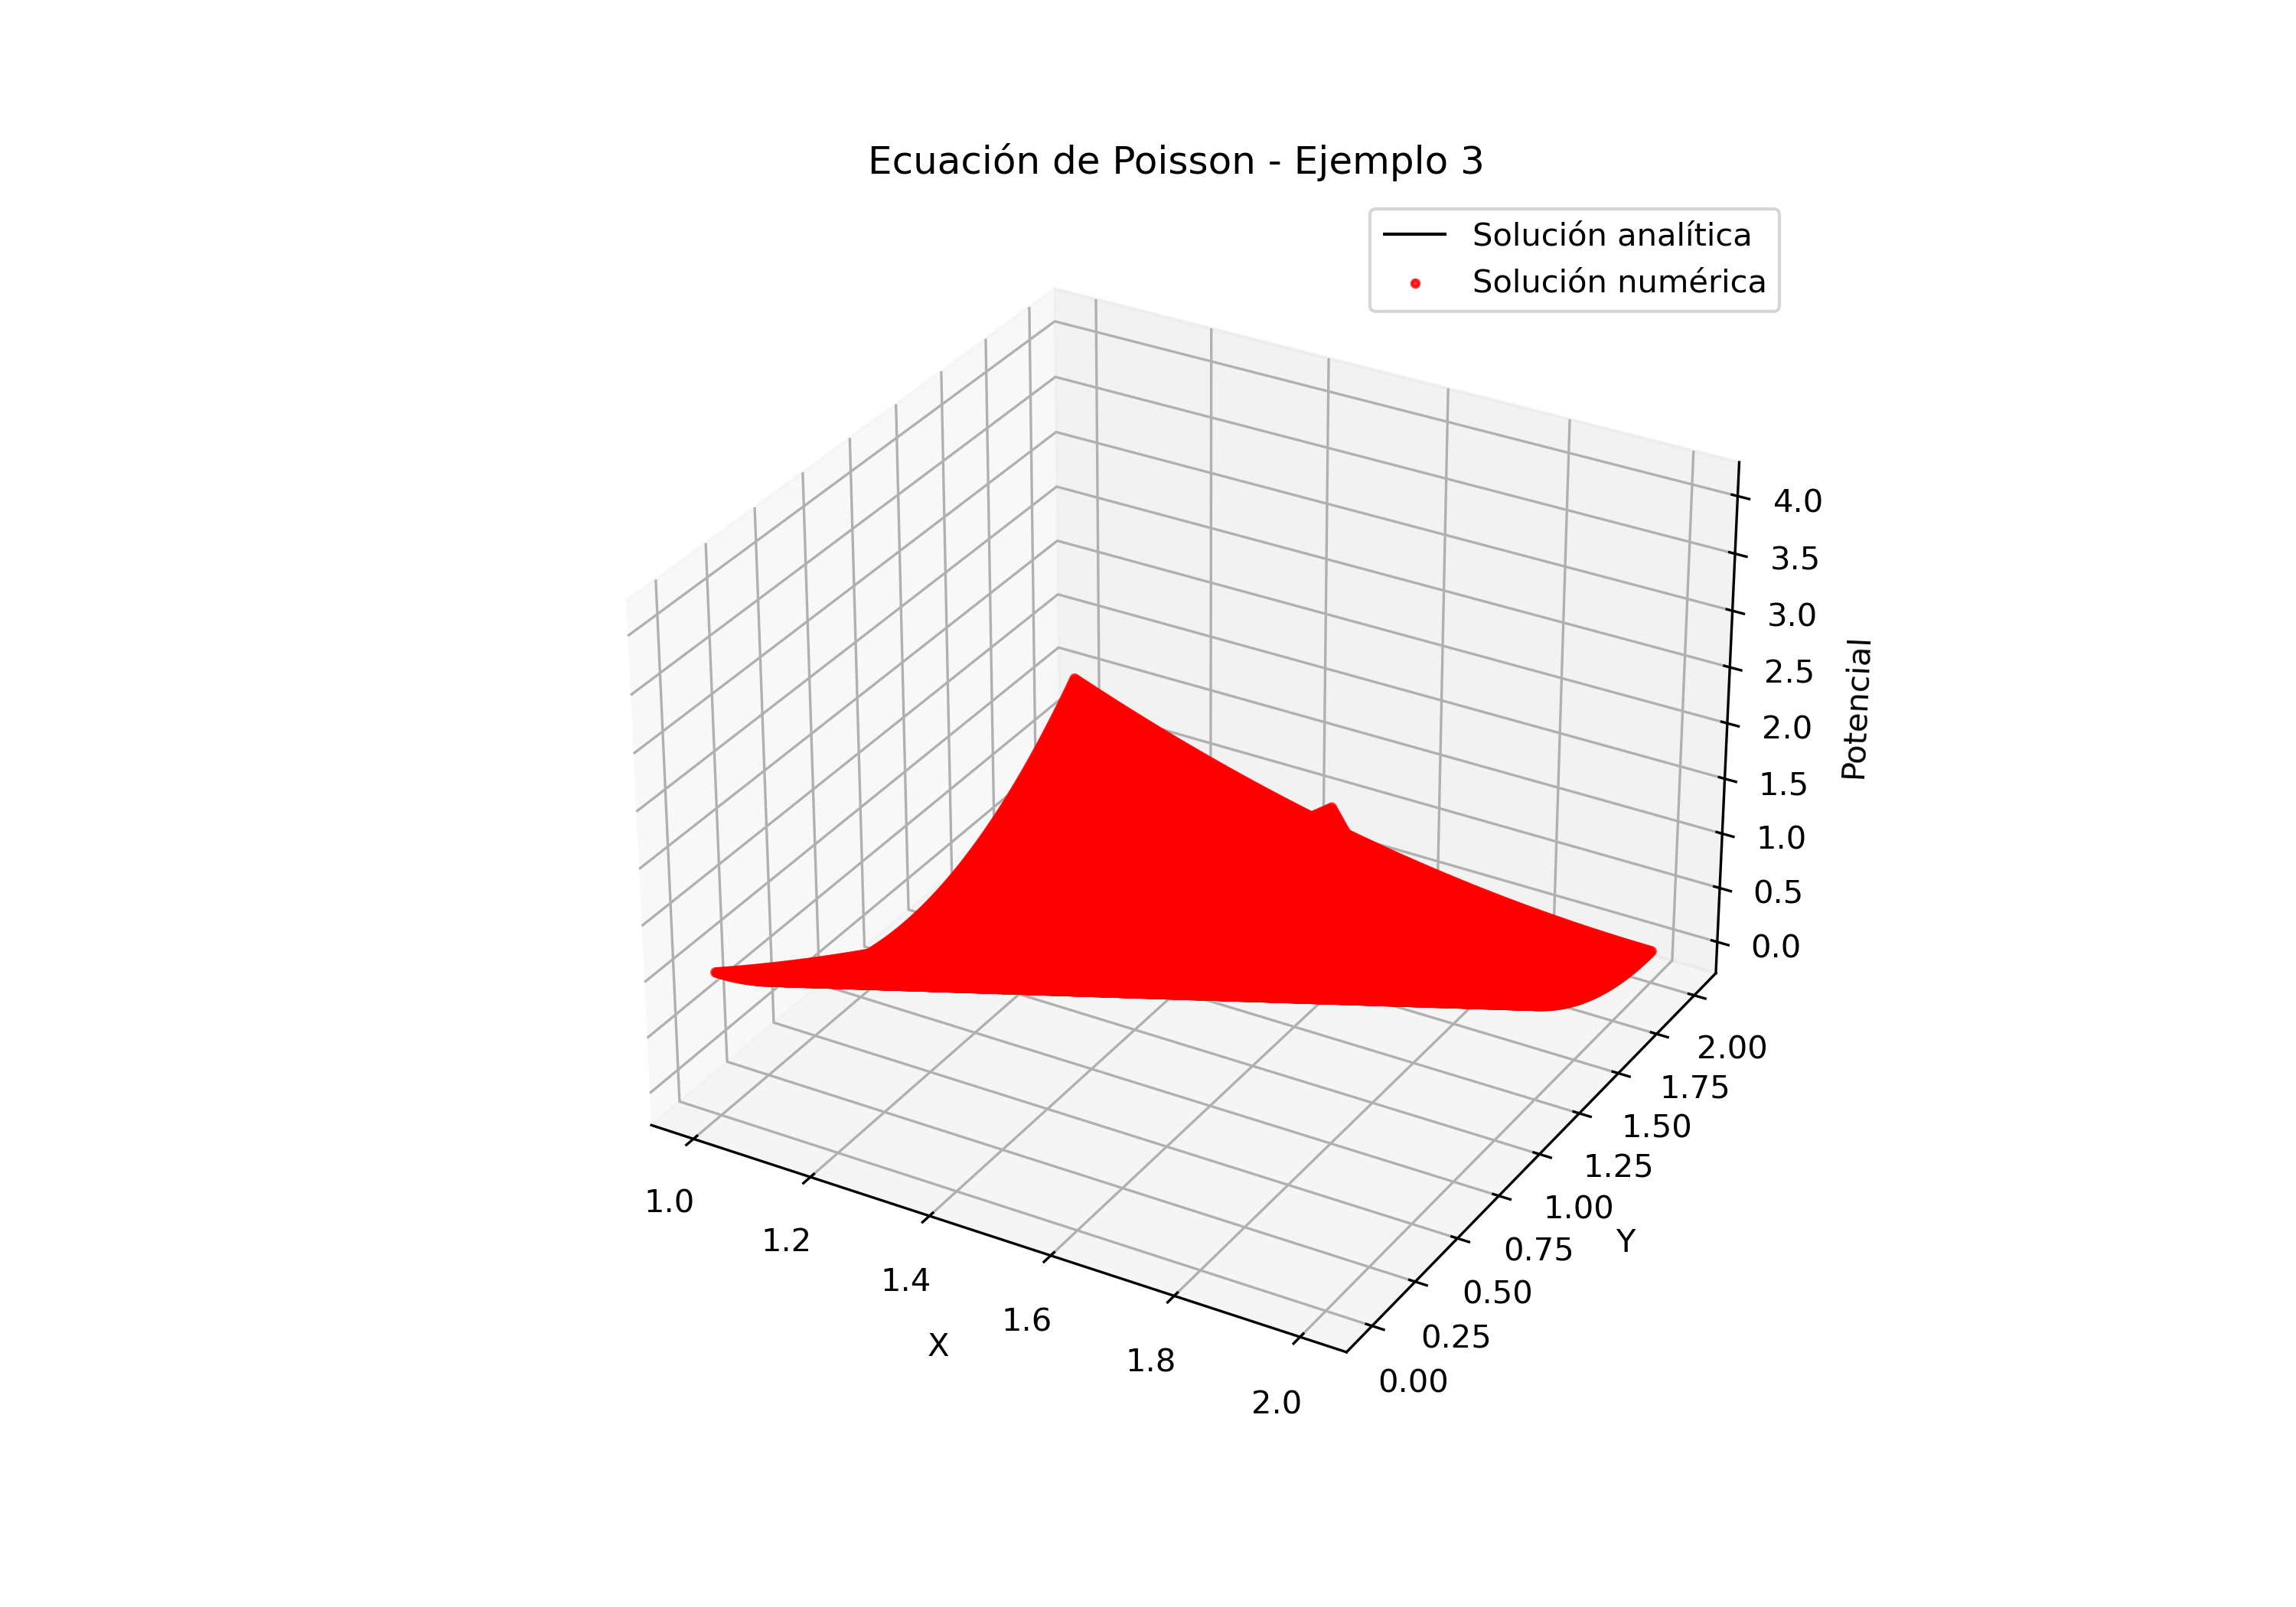
\includegraphics[width=0.8\textwidth]{imag/solucion_serial_Ej3.png}
    \caption{Ejemplo 3 resuelto con método secuencial.}
\end{figure}
\begin{figure}[H]
    \centering
    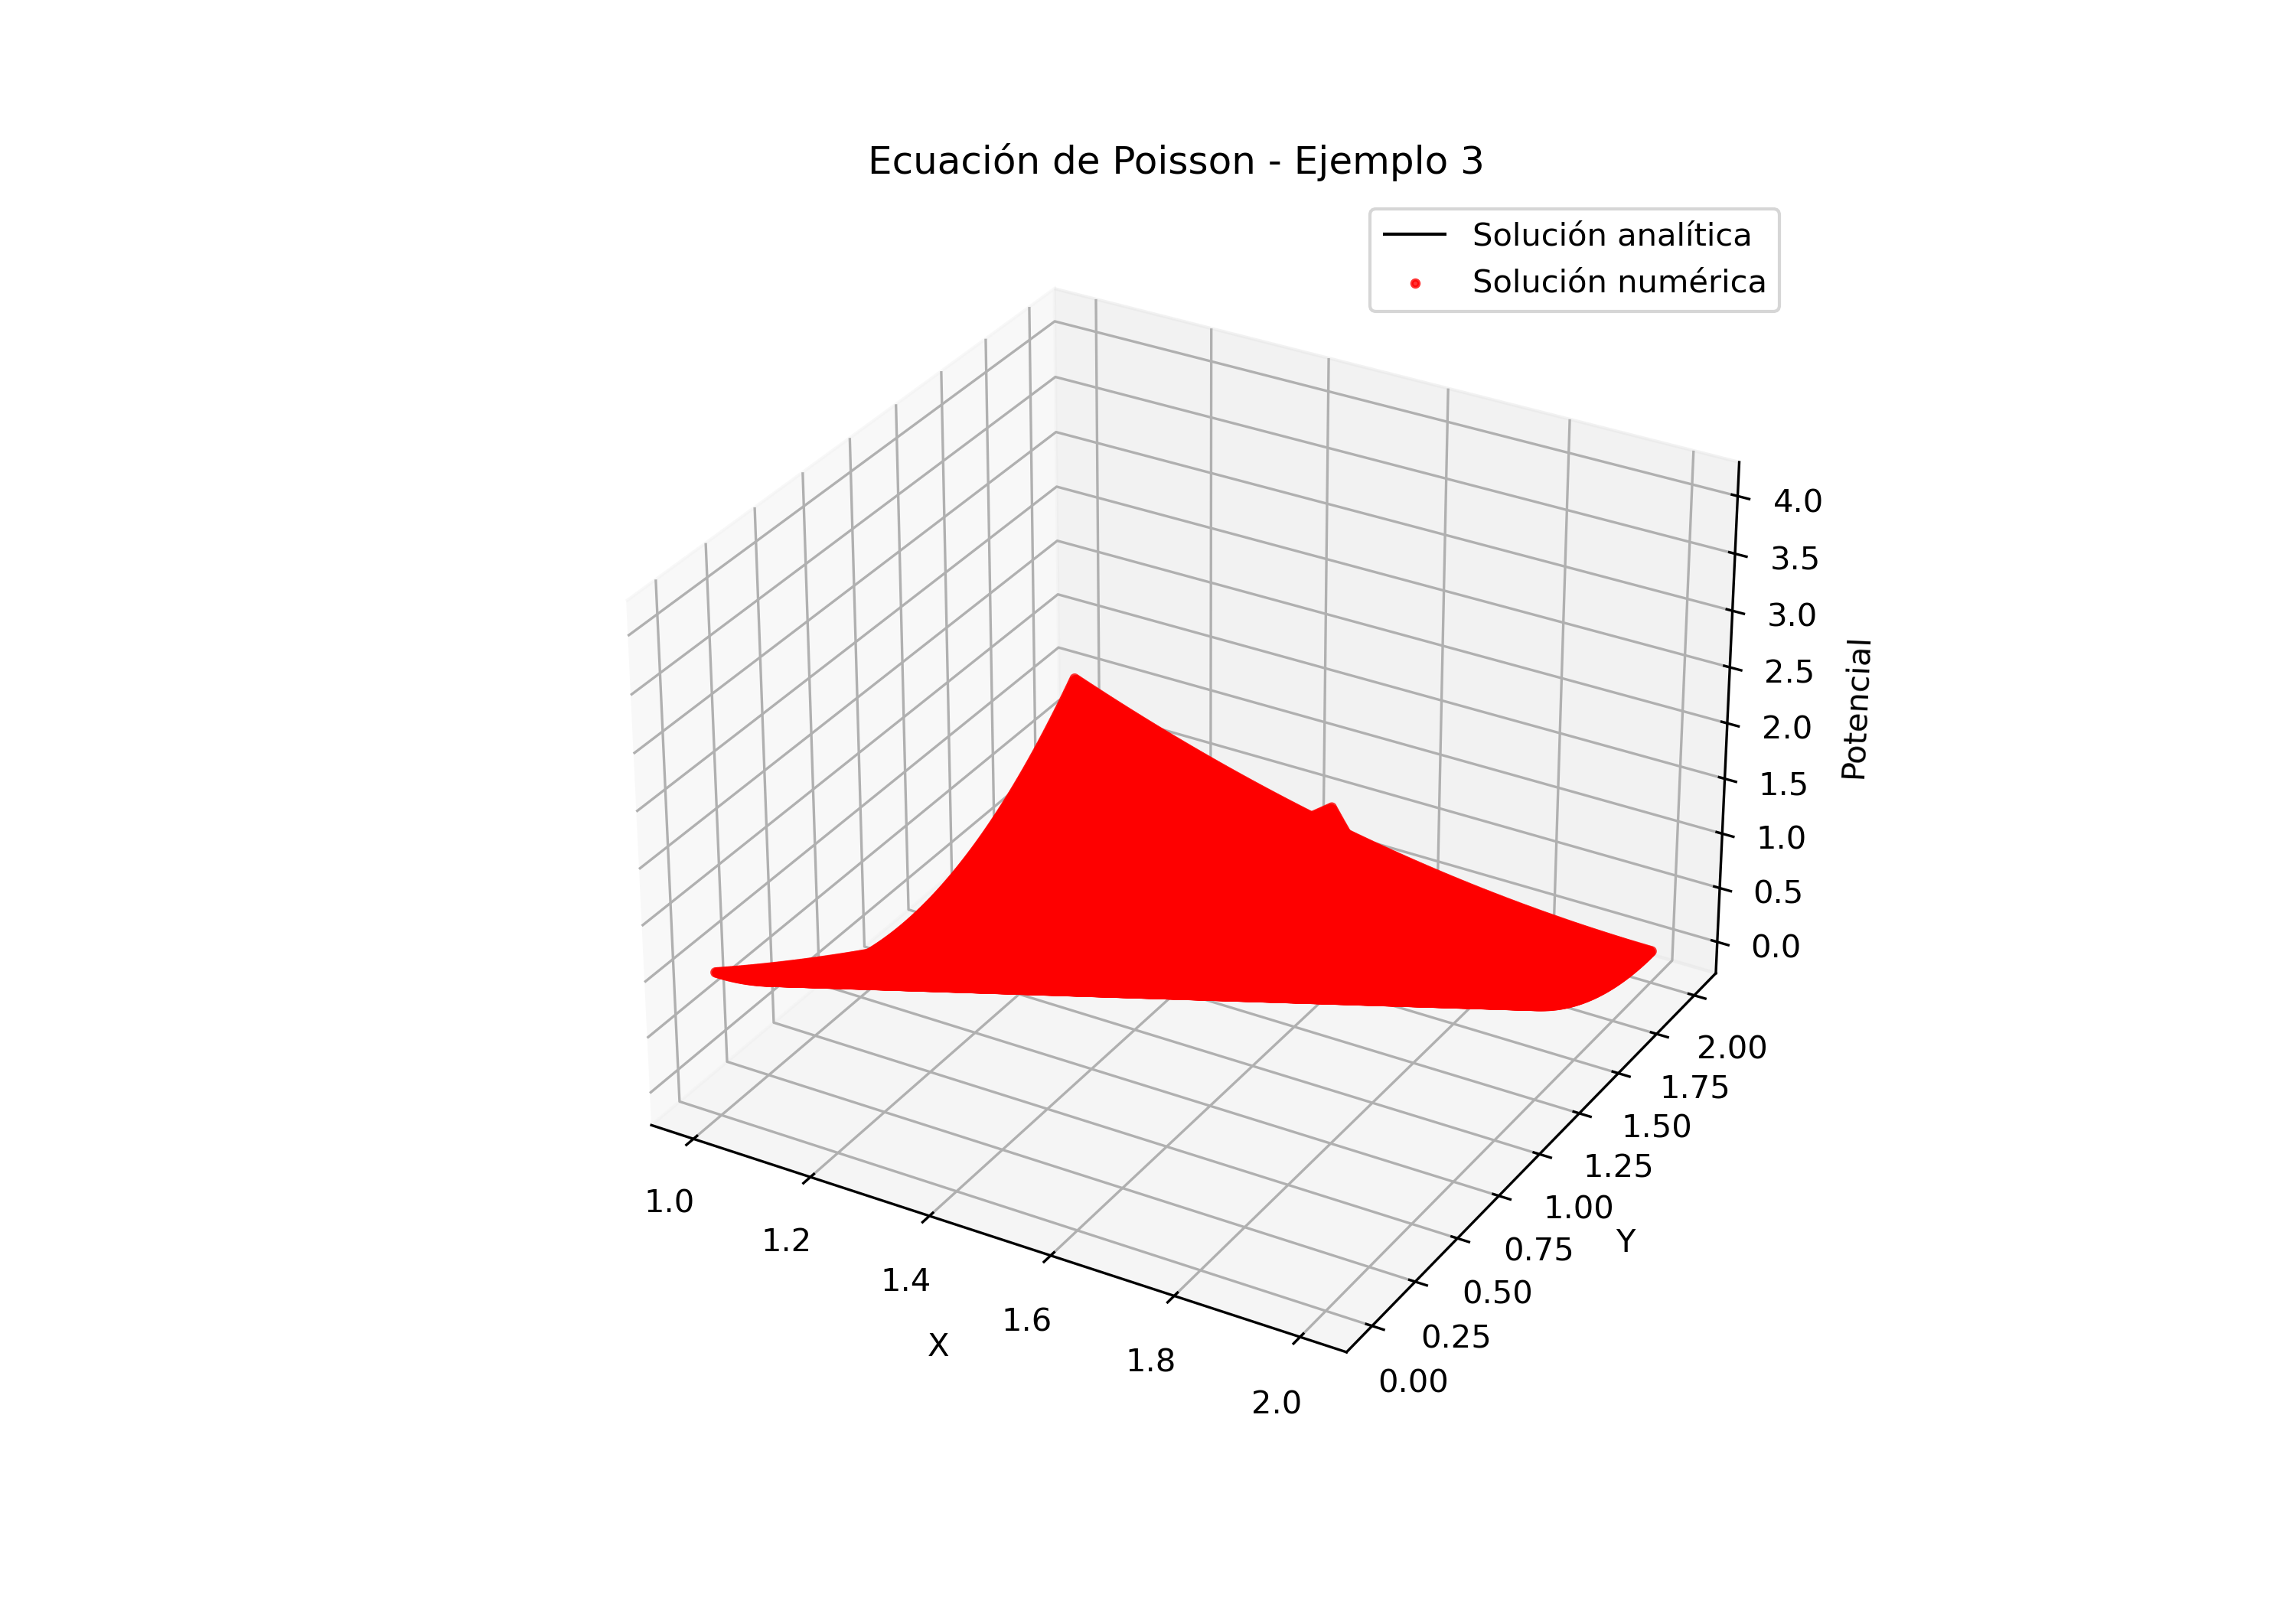
\includegraphics[width=0.8\textwidth]{imag/solucion_parallel_for_Ej3.png}
    \caption{Ejemplo 3 resuelto con \texttt{parallel for collapse}.}
\end{figure}
\begin{figure}[H]
    \centering
    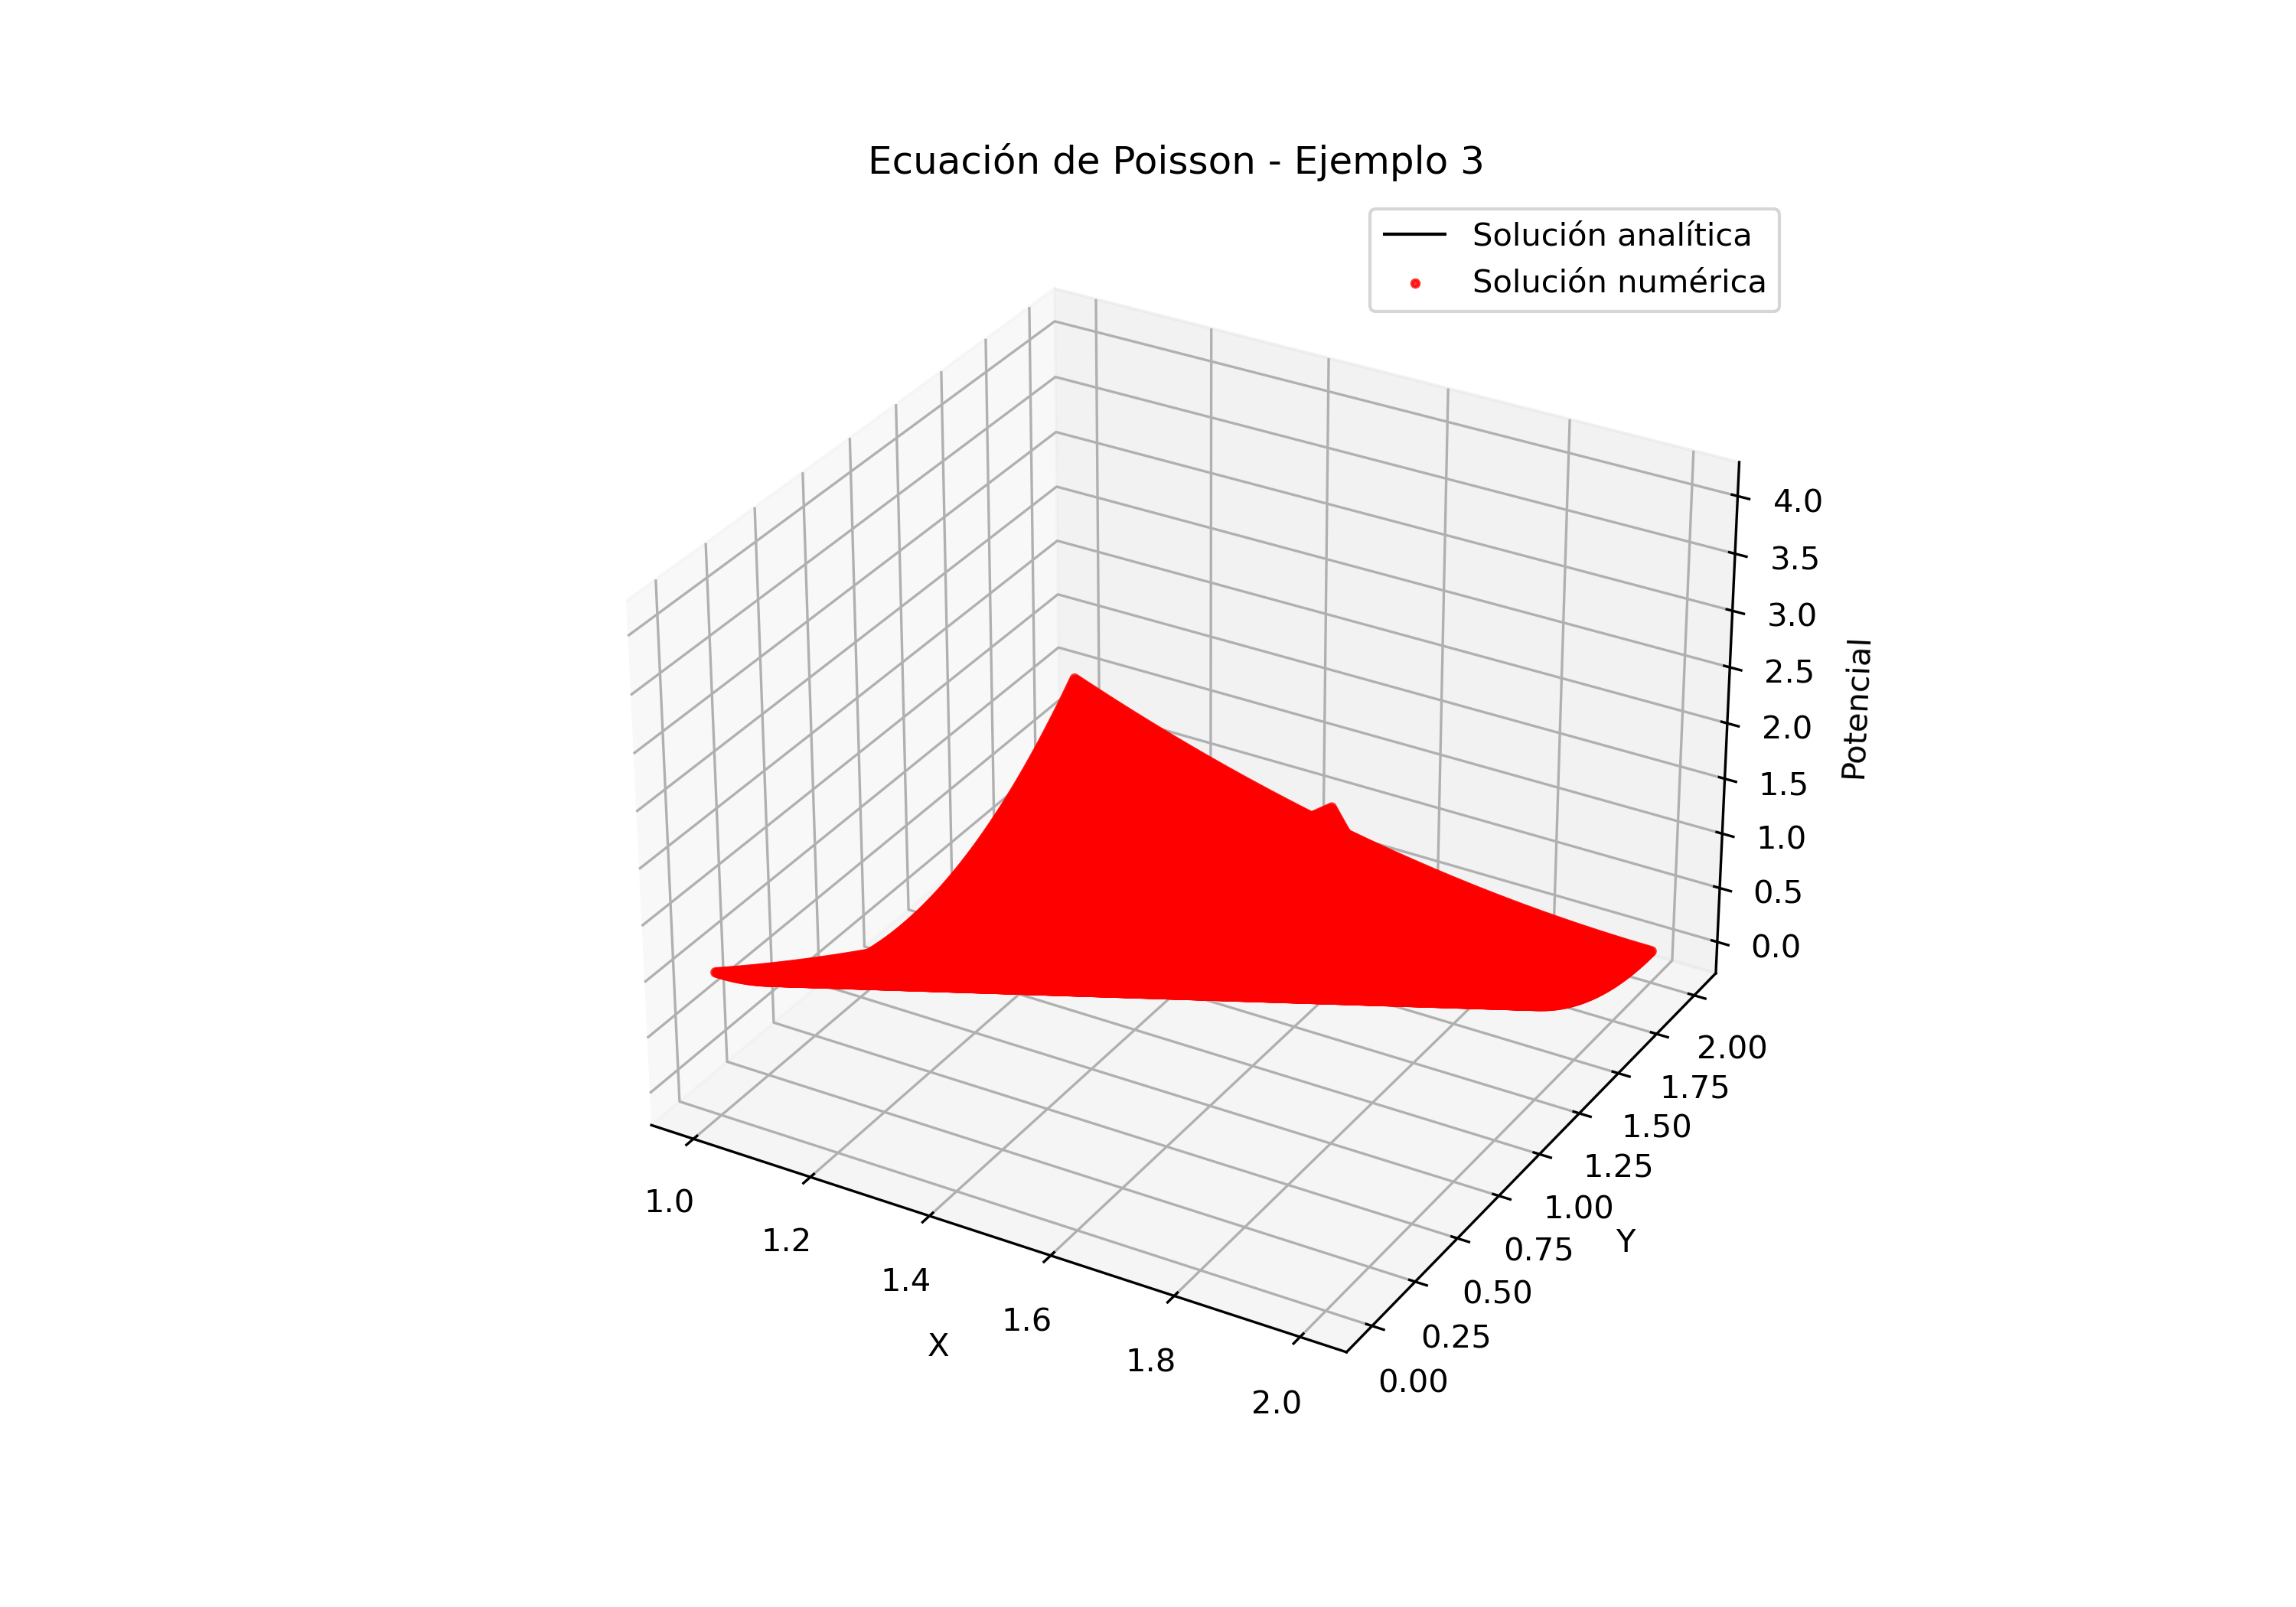
\includegraphics[width=0.8\textwidth]{imag/solucion_critical_Ej3.png}
    \caption{Ejemplo 3 resuelto con \texttt{critical}.}
\end{figure}
\begin{figure}[H]
    \centering
    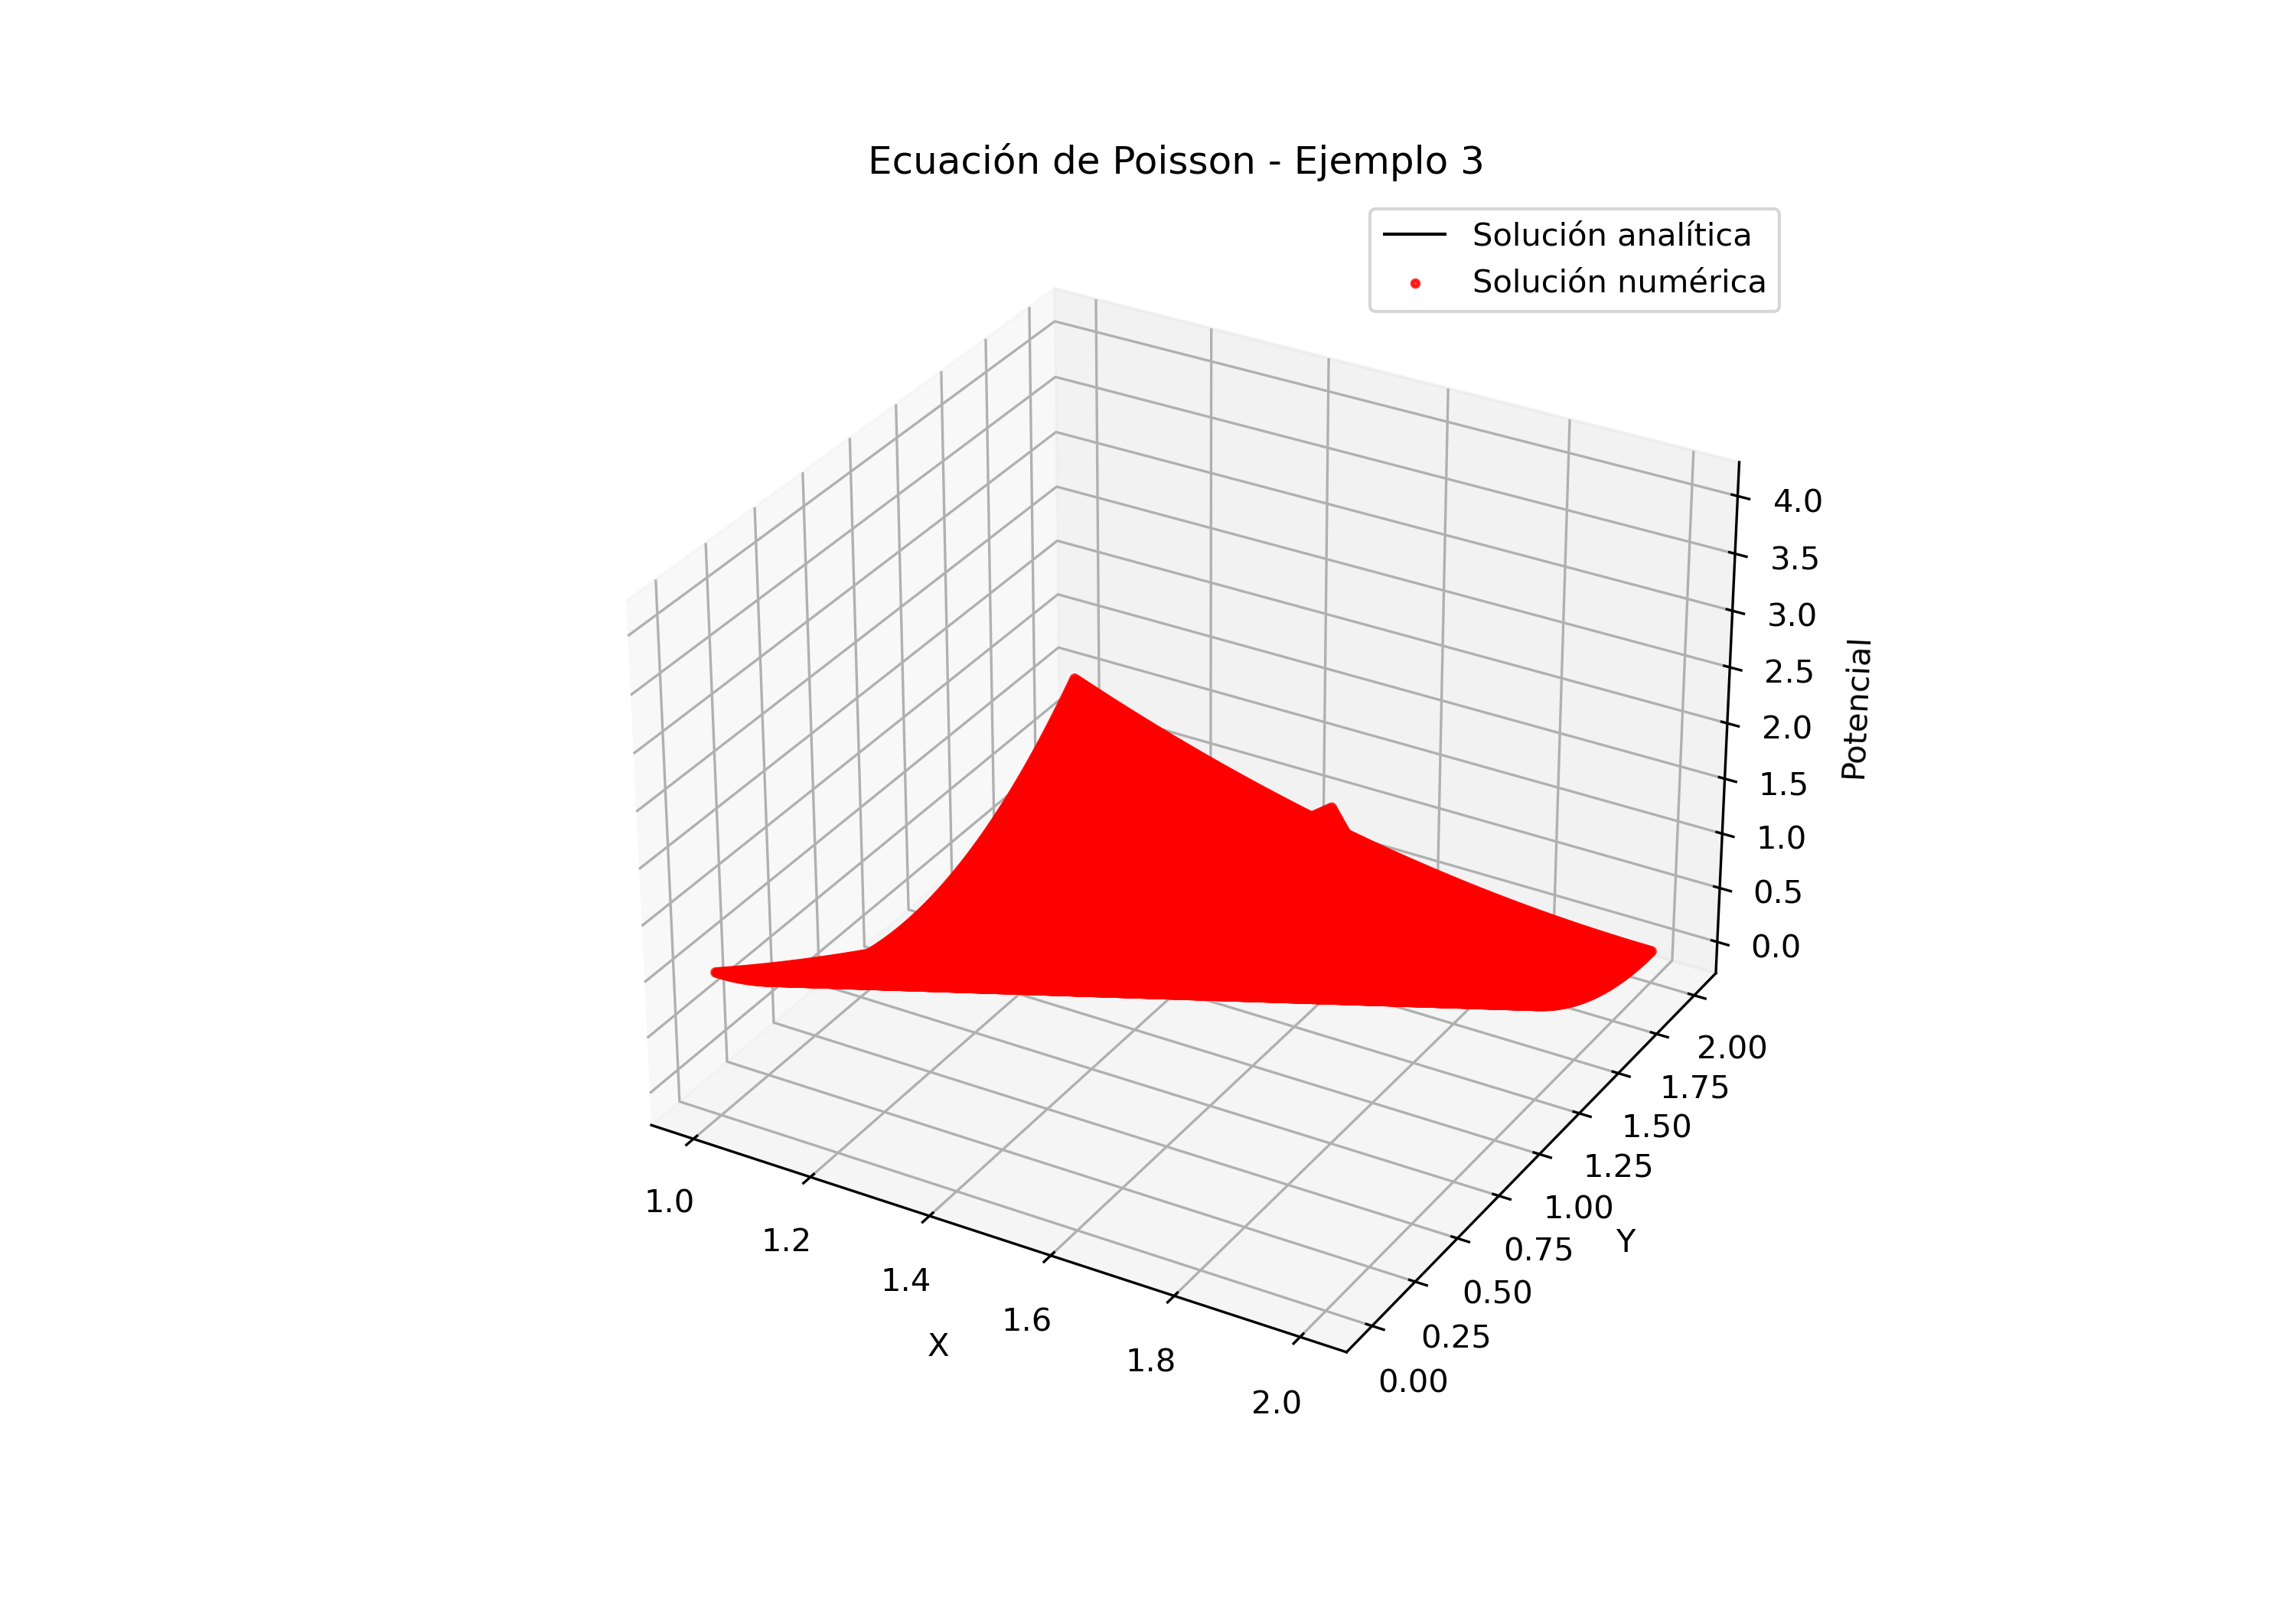
\includegraphics[width=0.8\textwidth]{imag/solucion_atomic_Ej3.png}
    \caption{Ejemplo 3 resuelto con \texttt{atomic}.}
\end{figure}
\begin{figure}[H]
    \centering
    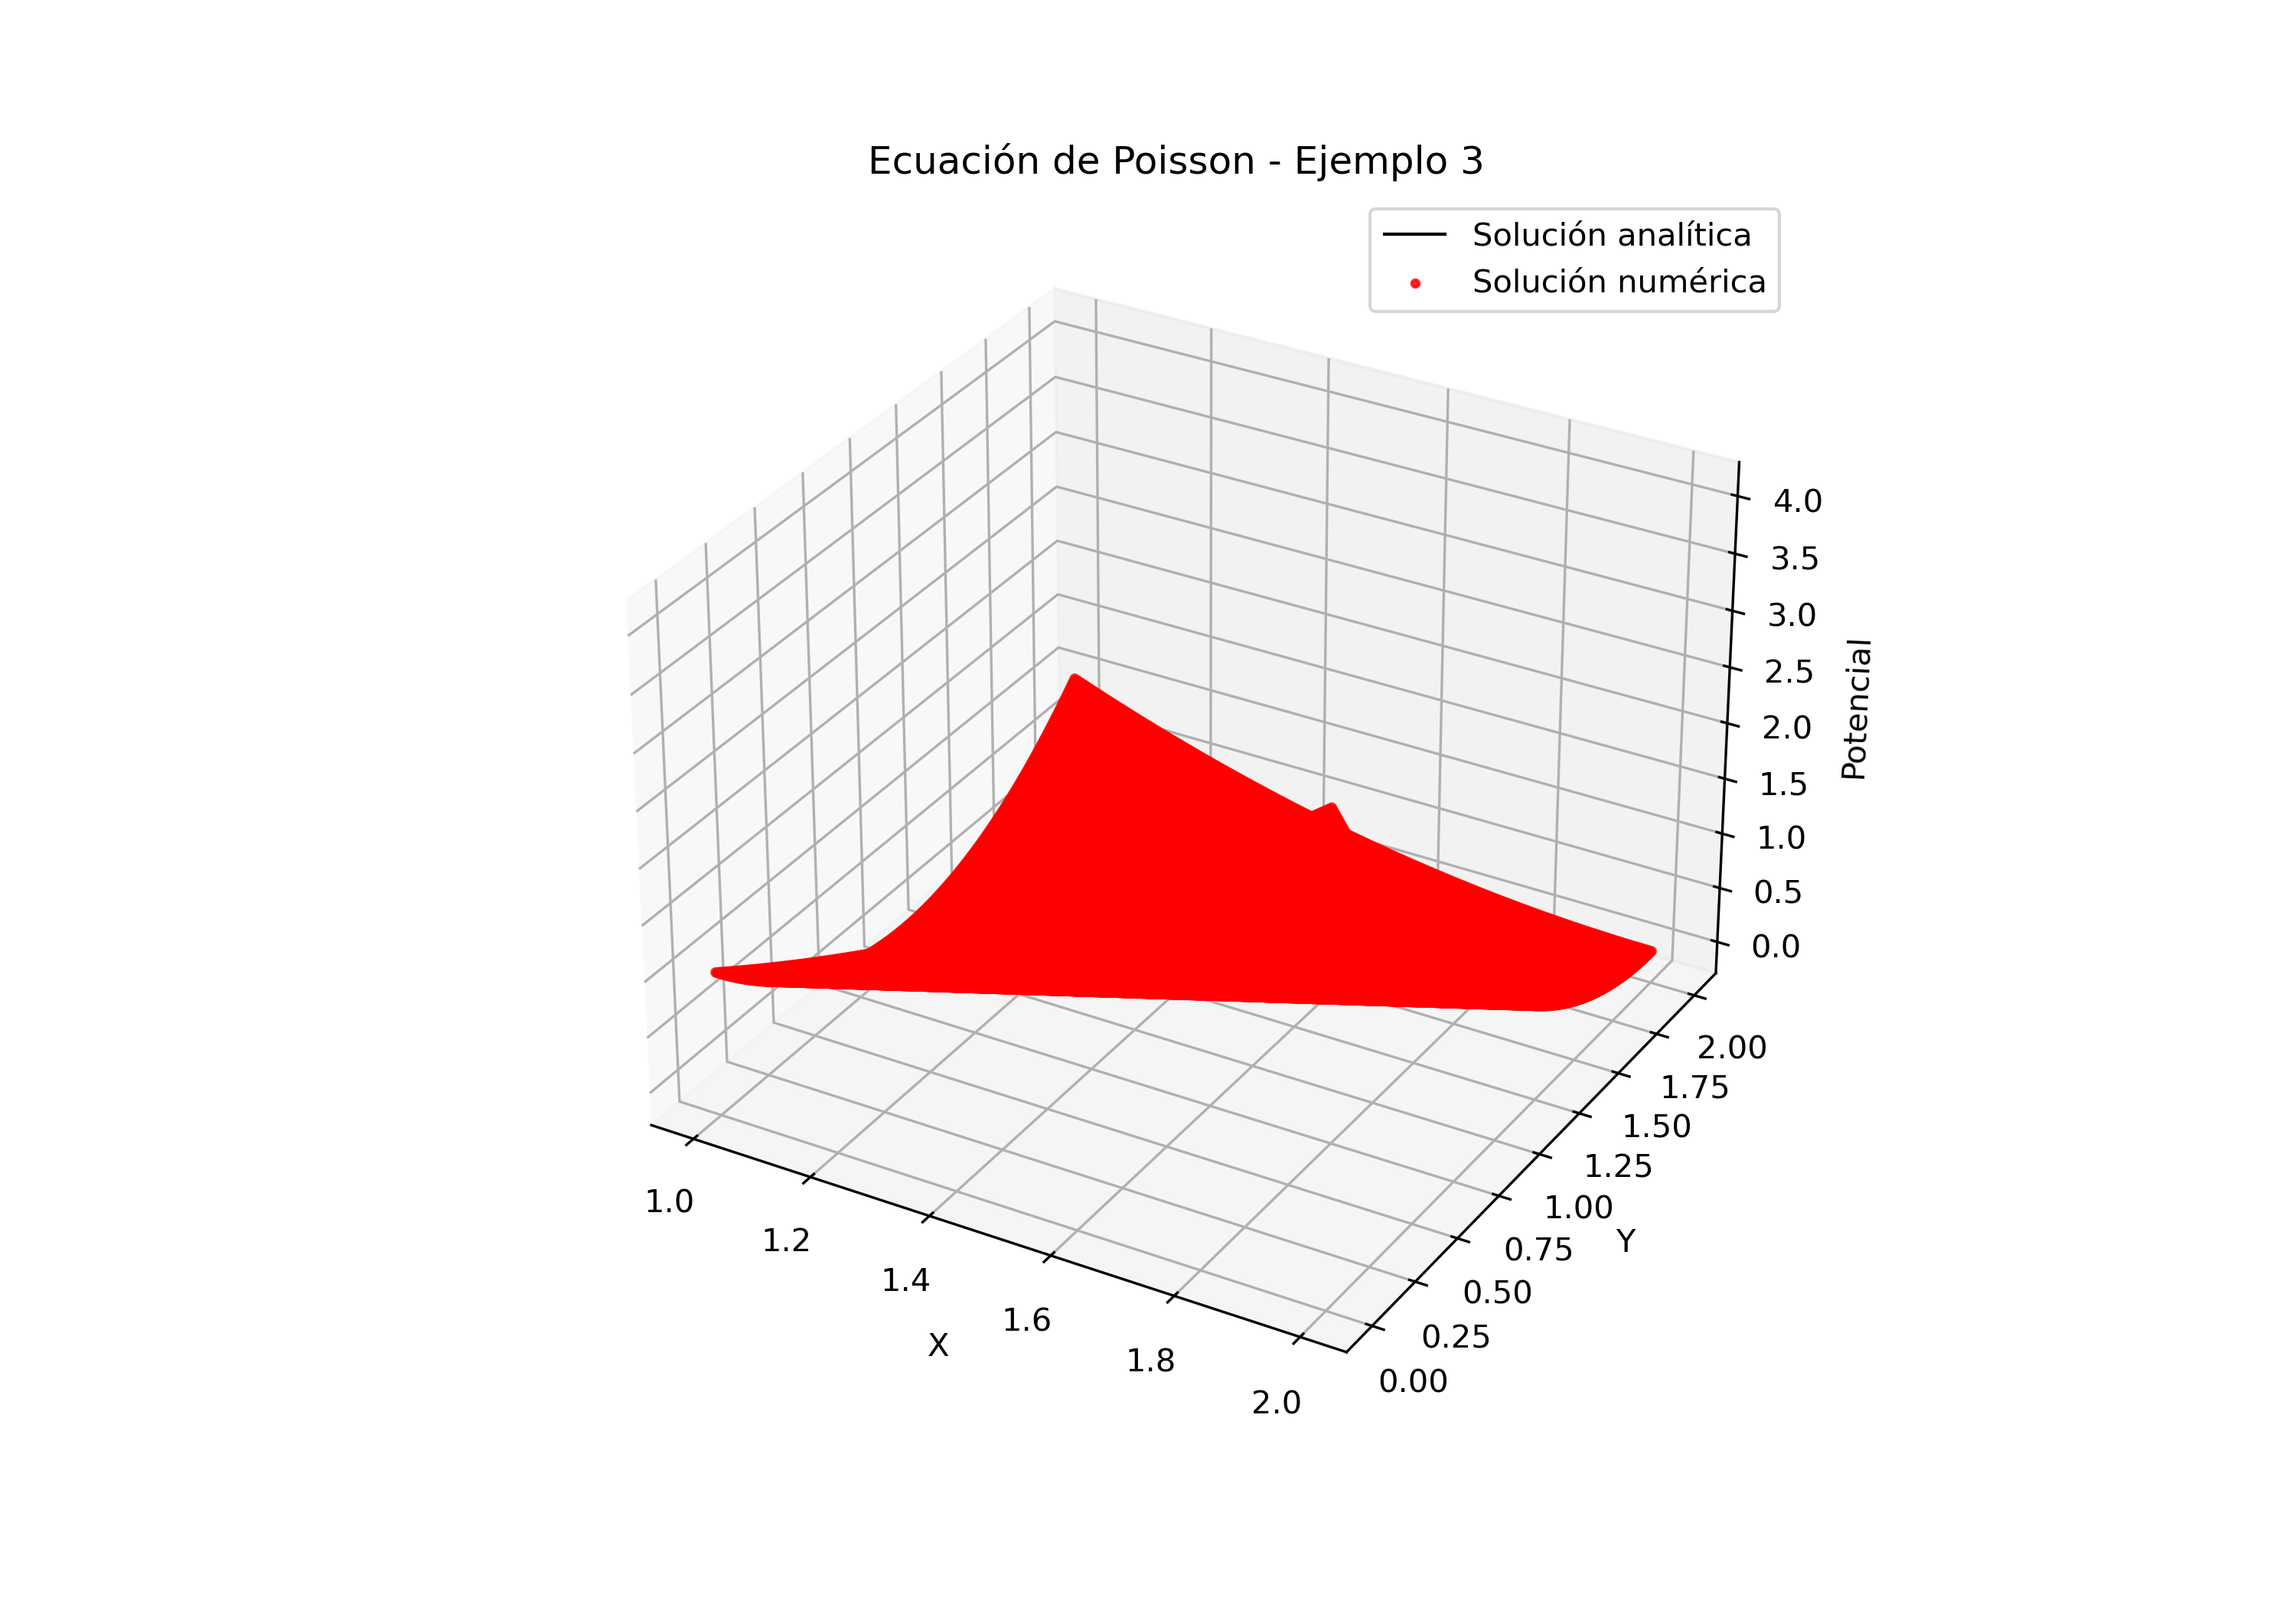
\includegraphics[width=0.8\textwidth]{imag/solucion_task_Ej3.png}
    \caption{Ejemplo 3 resuelto con \texttt{task}.}
\end{figure}

% === EJEMPLO 4 ===
\begin{figure}[H]
    \centering
    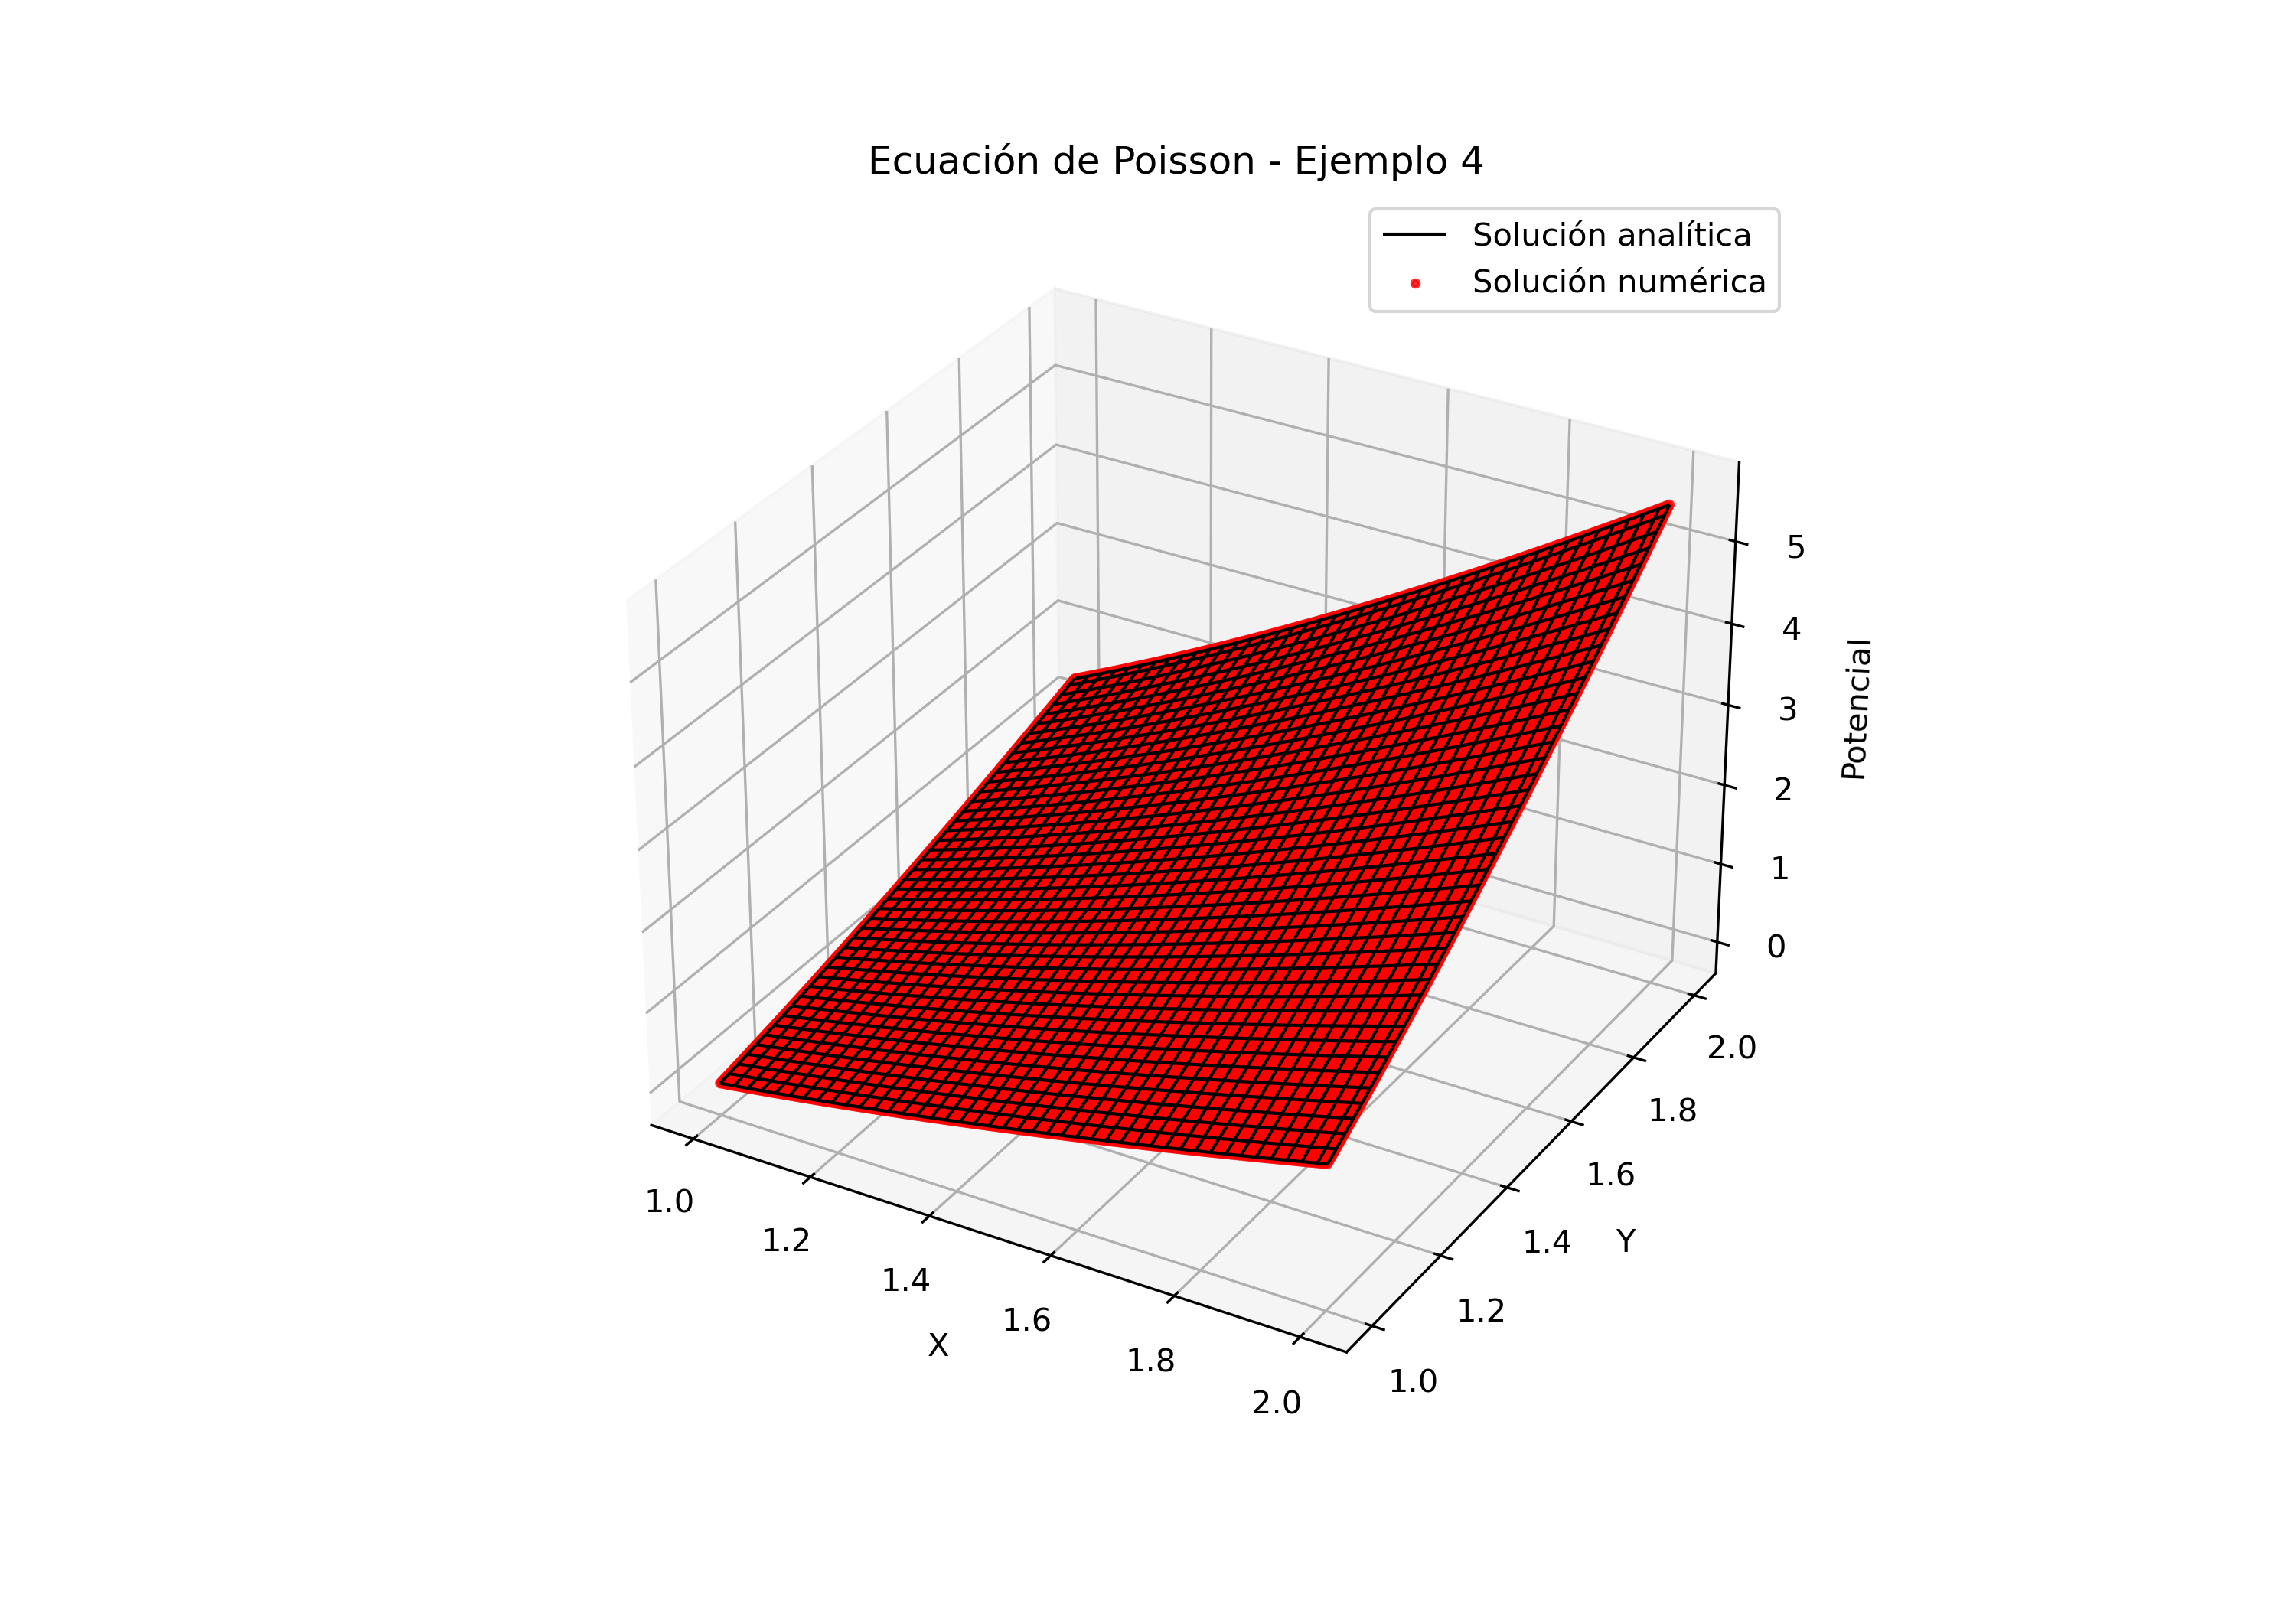
\includegraphics[width=0.8\textwidth]{imag/solucion_serial_Ej4.png}
    \caption{Ejemplo 4 resuelto con método secuencial.}
\end{figure}
\begin{figure}[H]
    \centering
    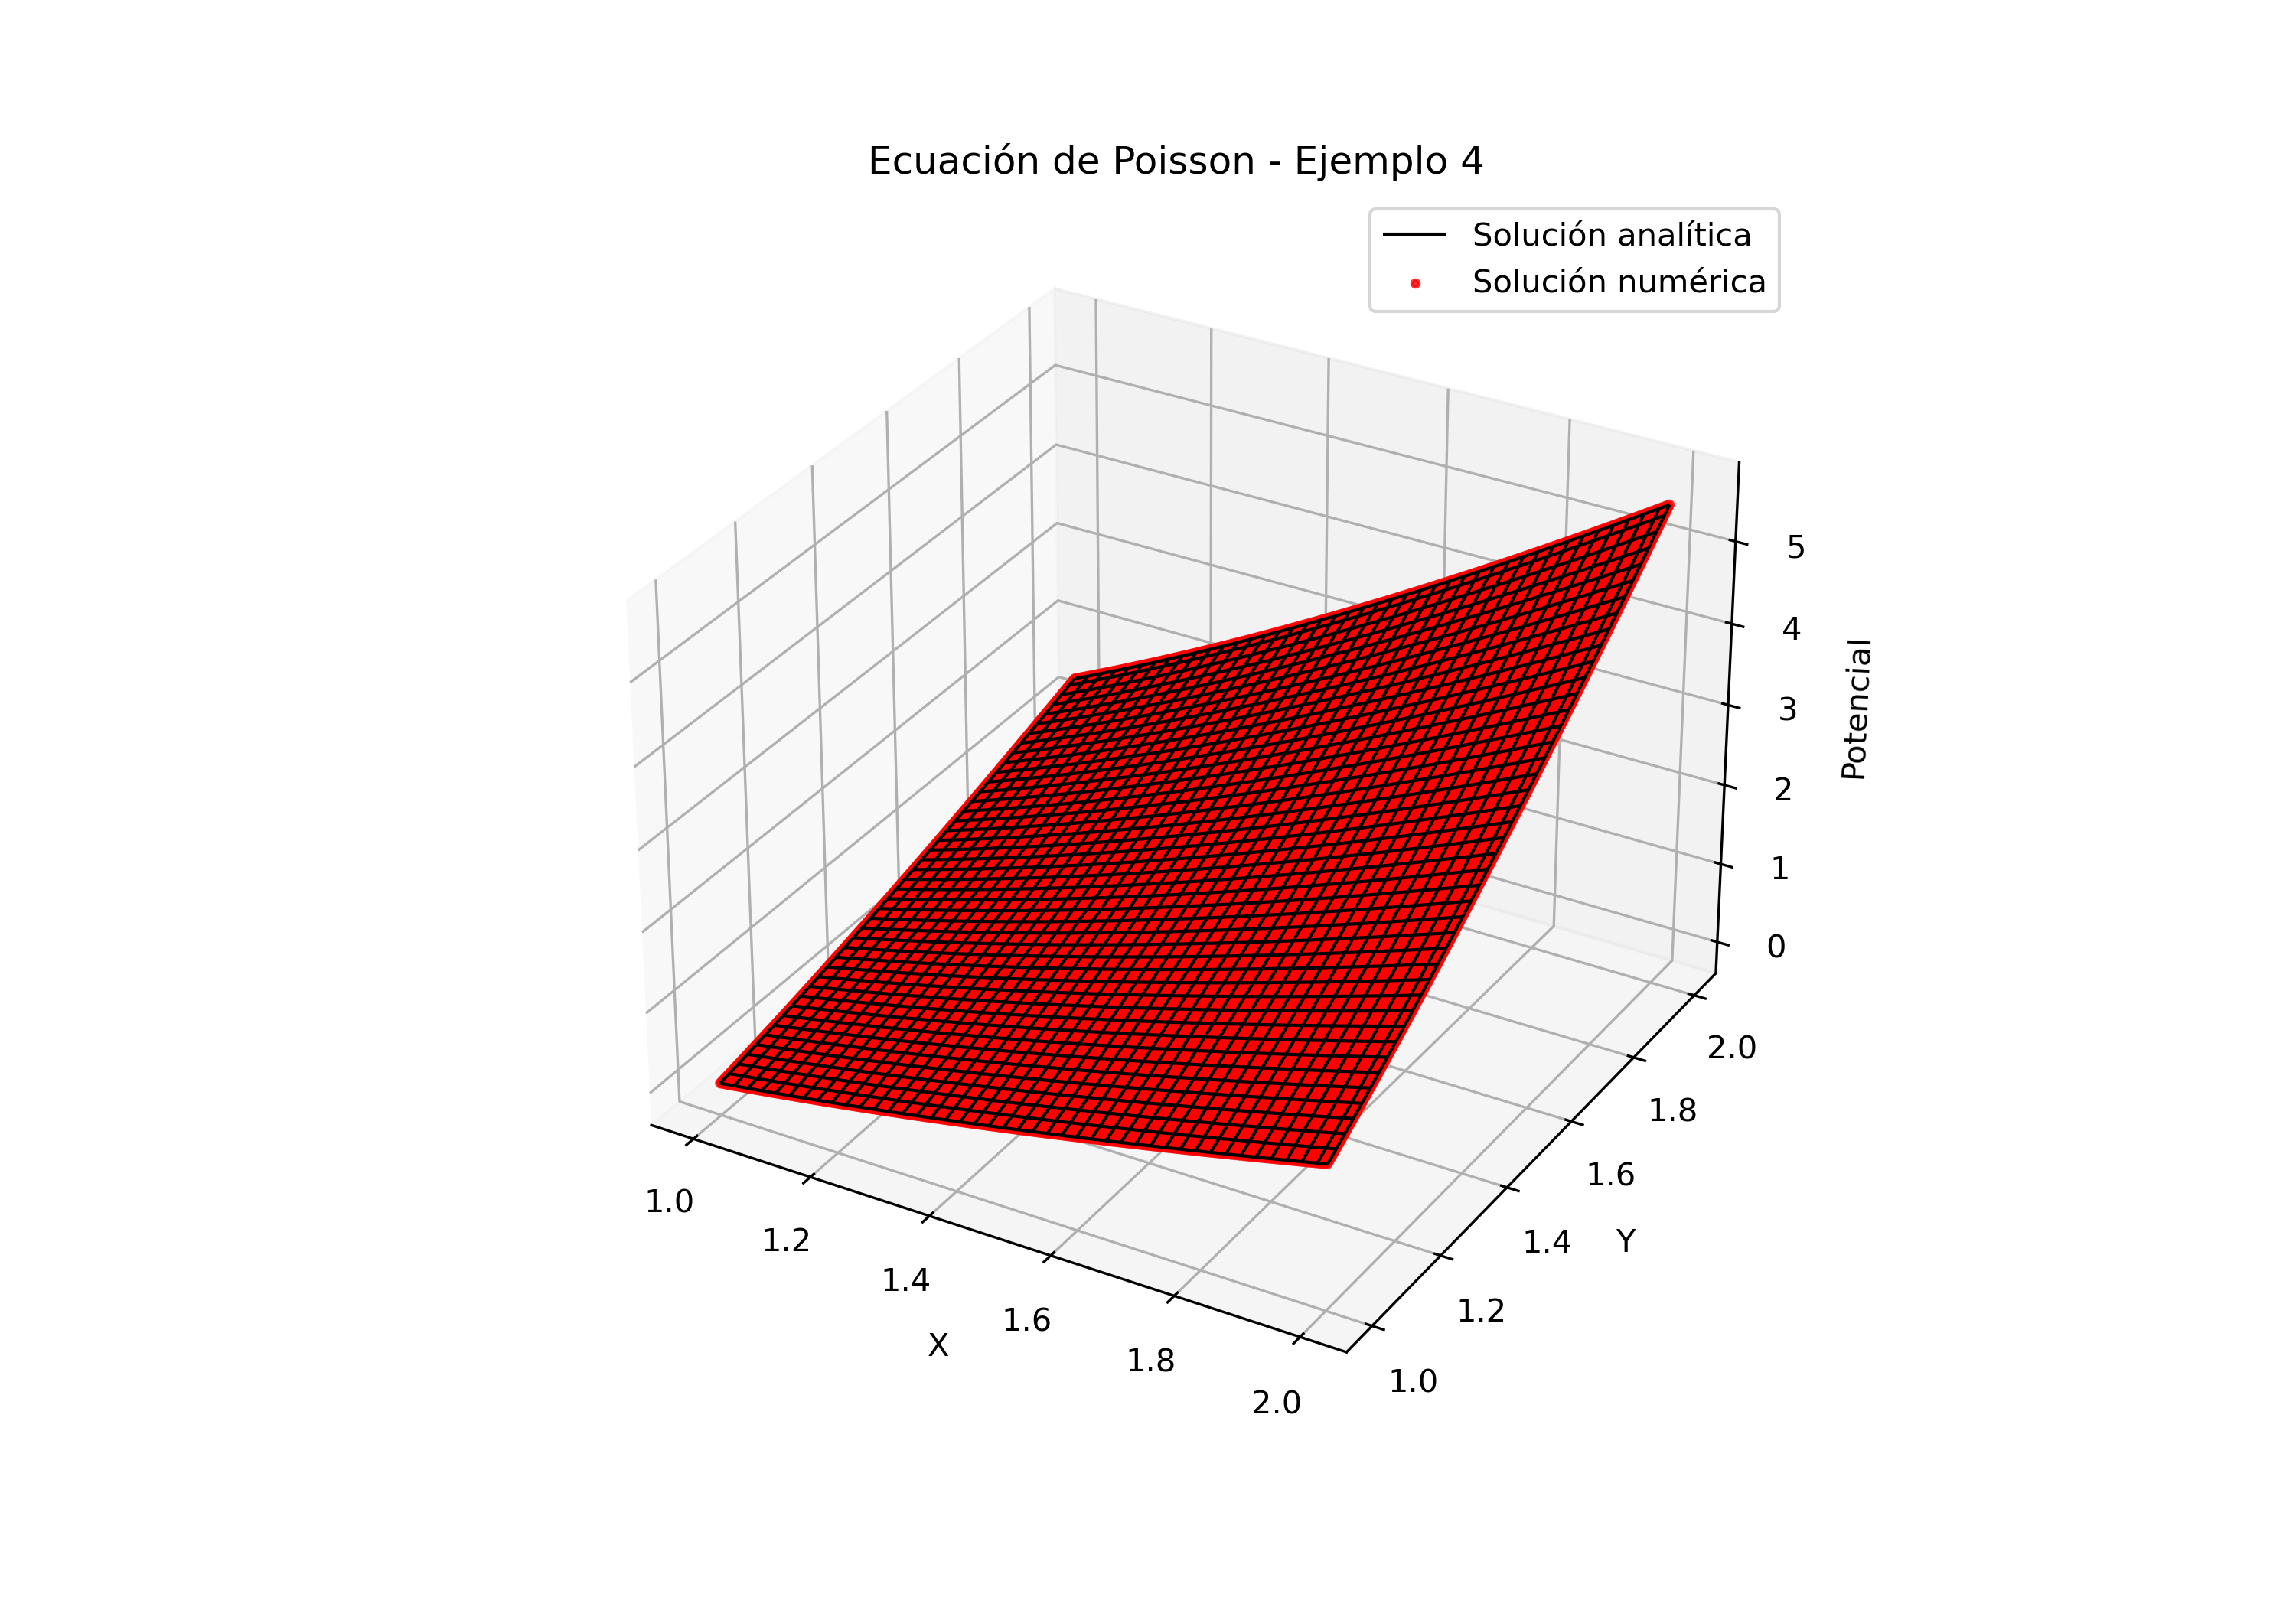
\includegraphics[width=0.8\textwidth]{imag/solucion_parallel_for_Ej4.png}
    \caption{Ejemplo 4 resuelto con \texttt{parallel for collapse}.}
\end{figure}
\begin{figure}[H]
    \centering
    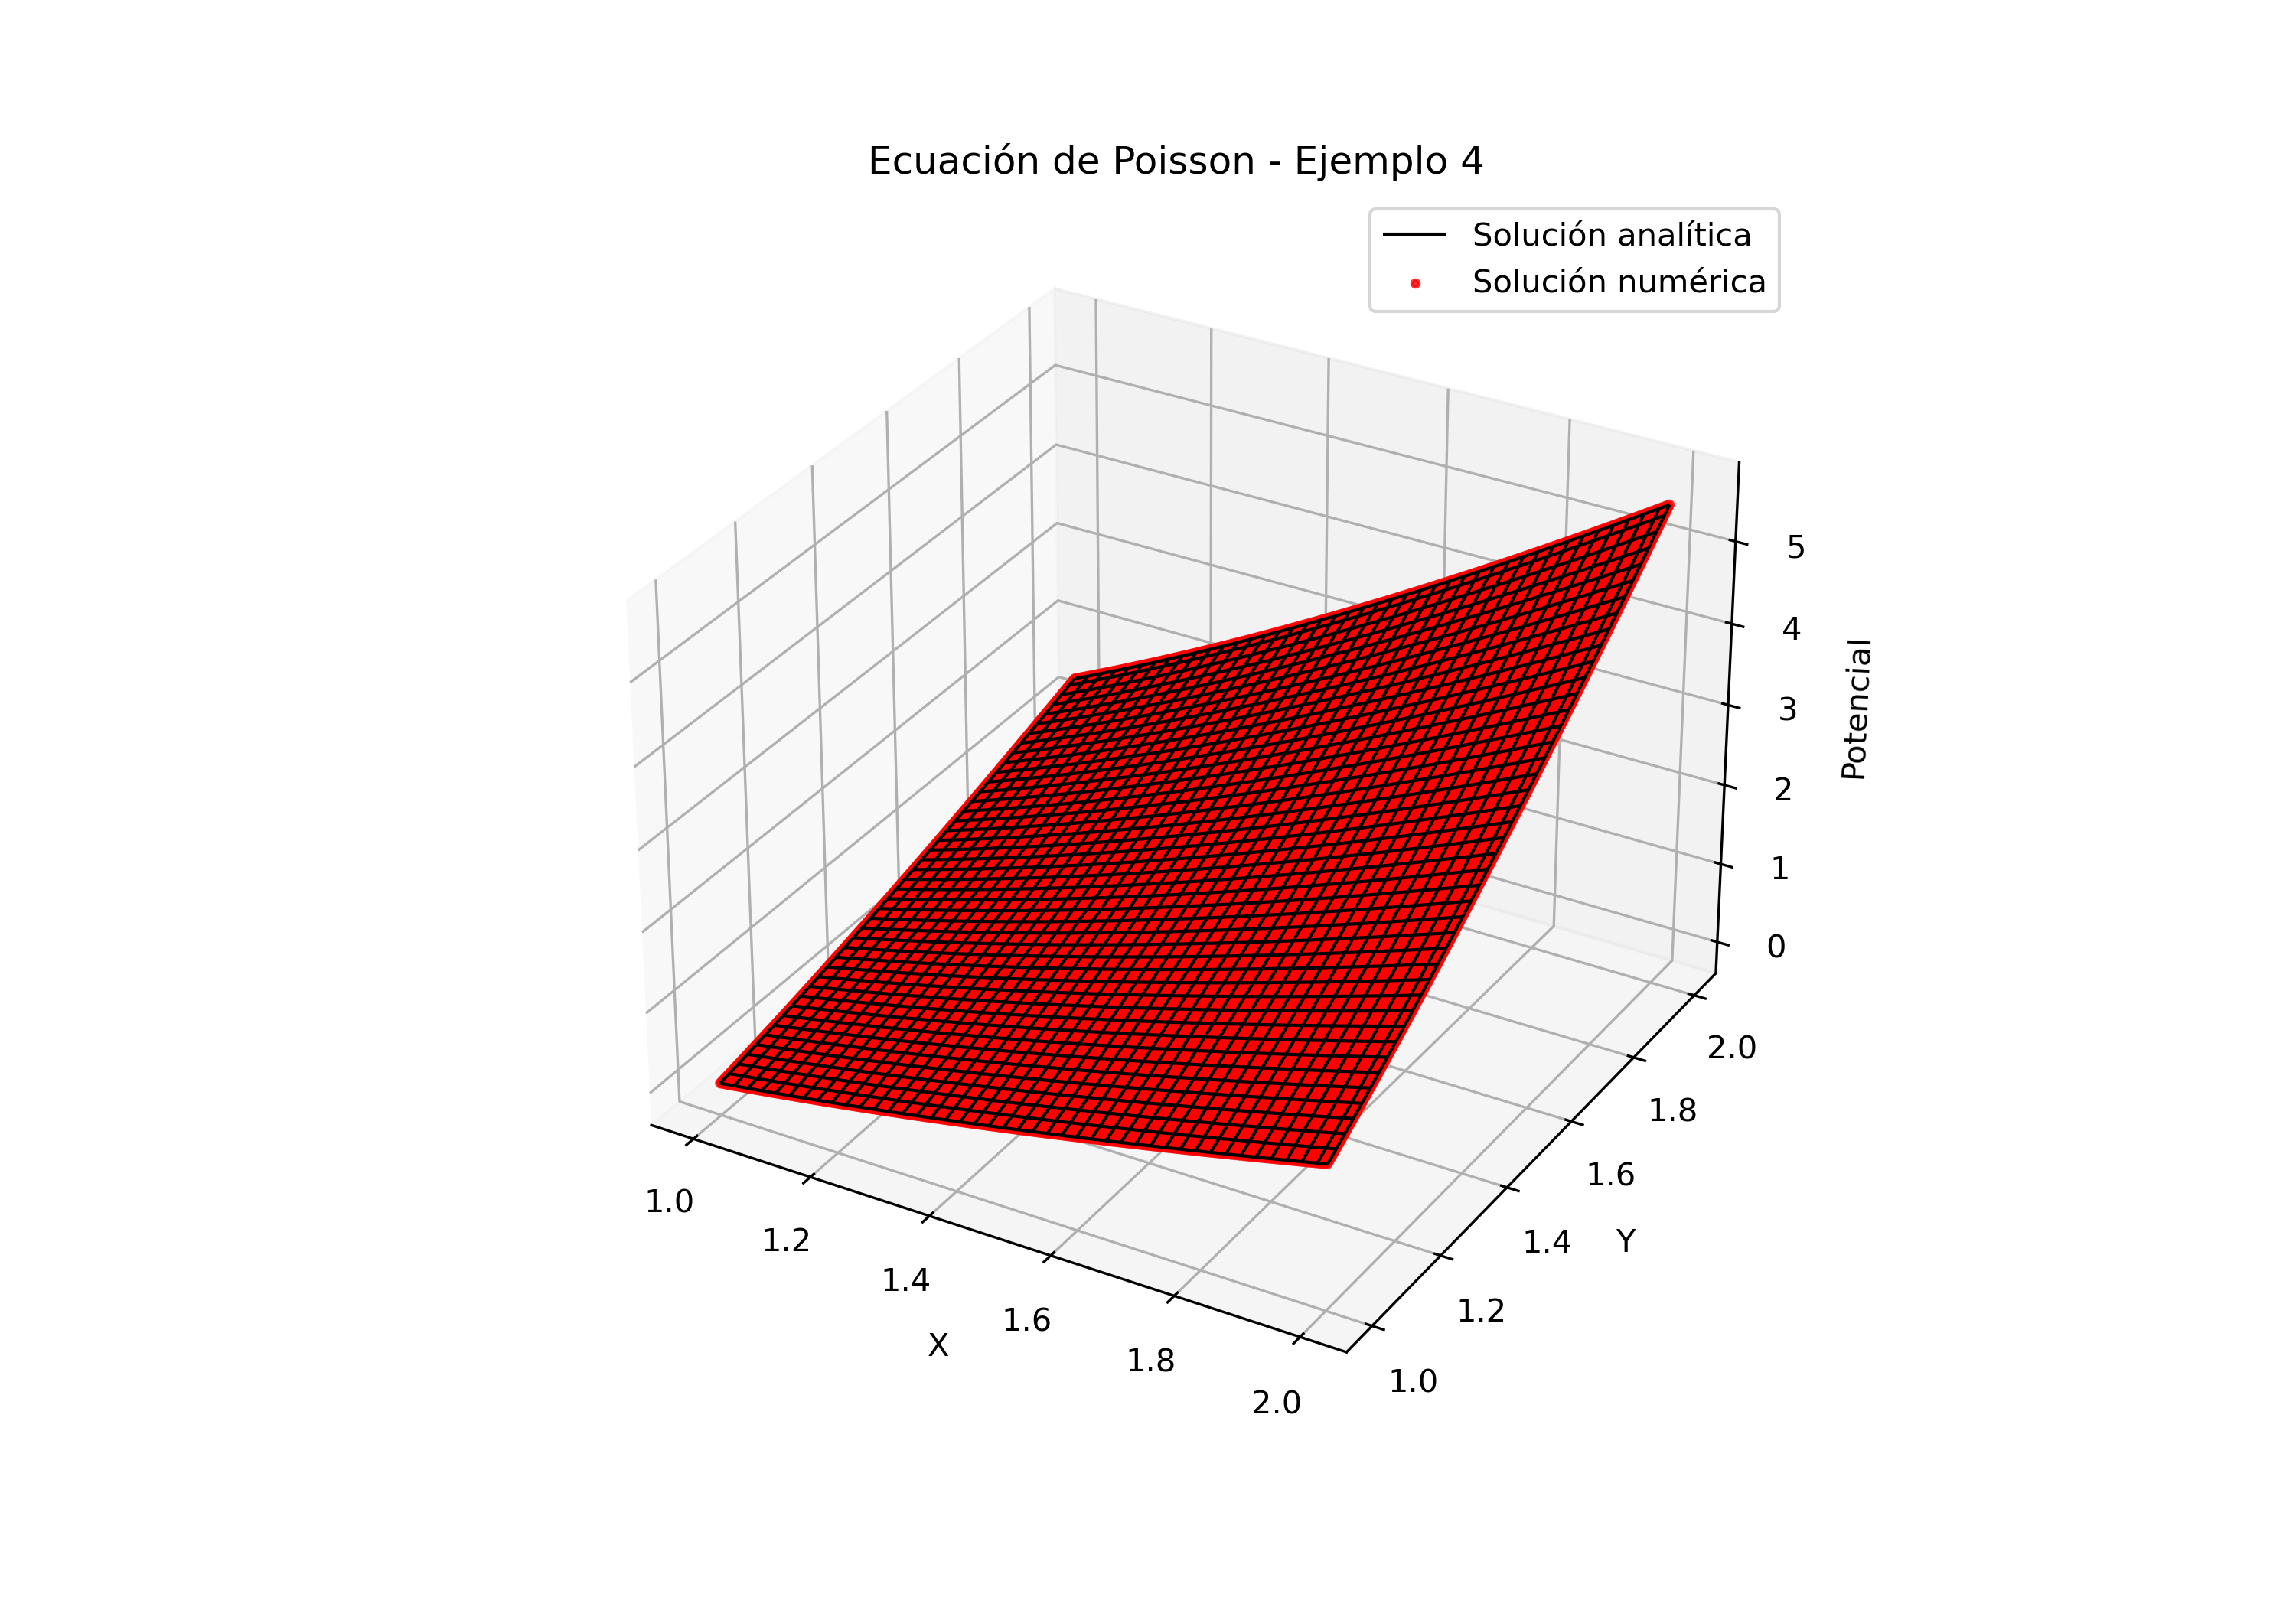
\includegraphics[width=0.8\textwidth]{imag/solucion_critical_Ej4.png}
    \caption{Ejemplo 4 resuelto con \texttt{critical}.}
\end{figure}
\begin{figure}[H]
    \centering
    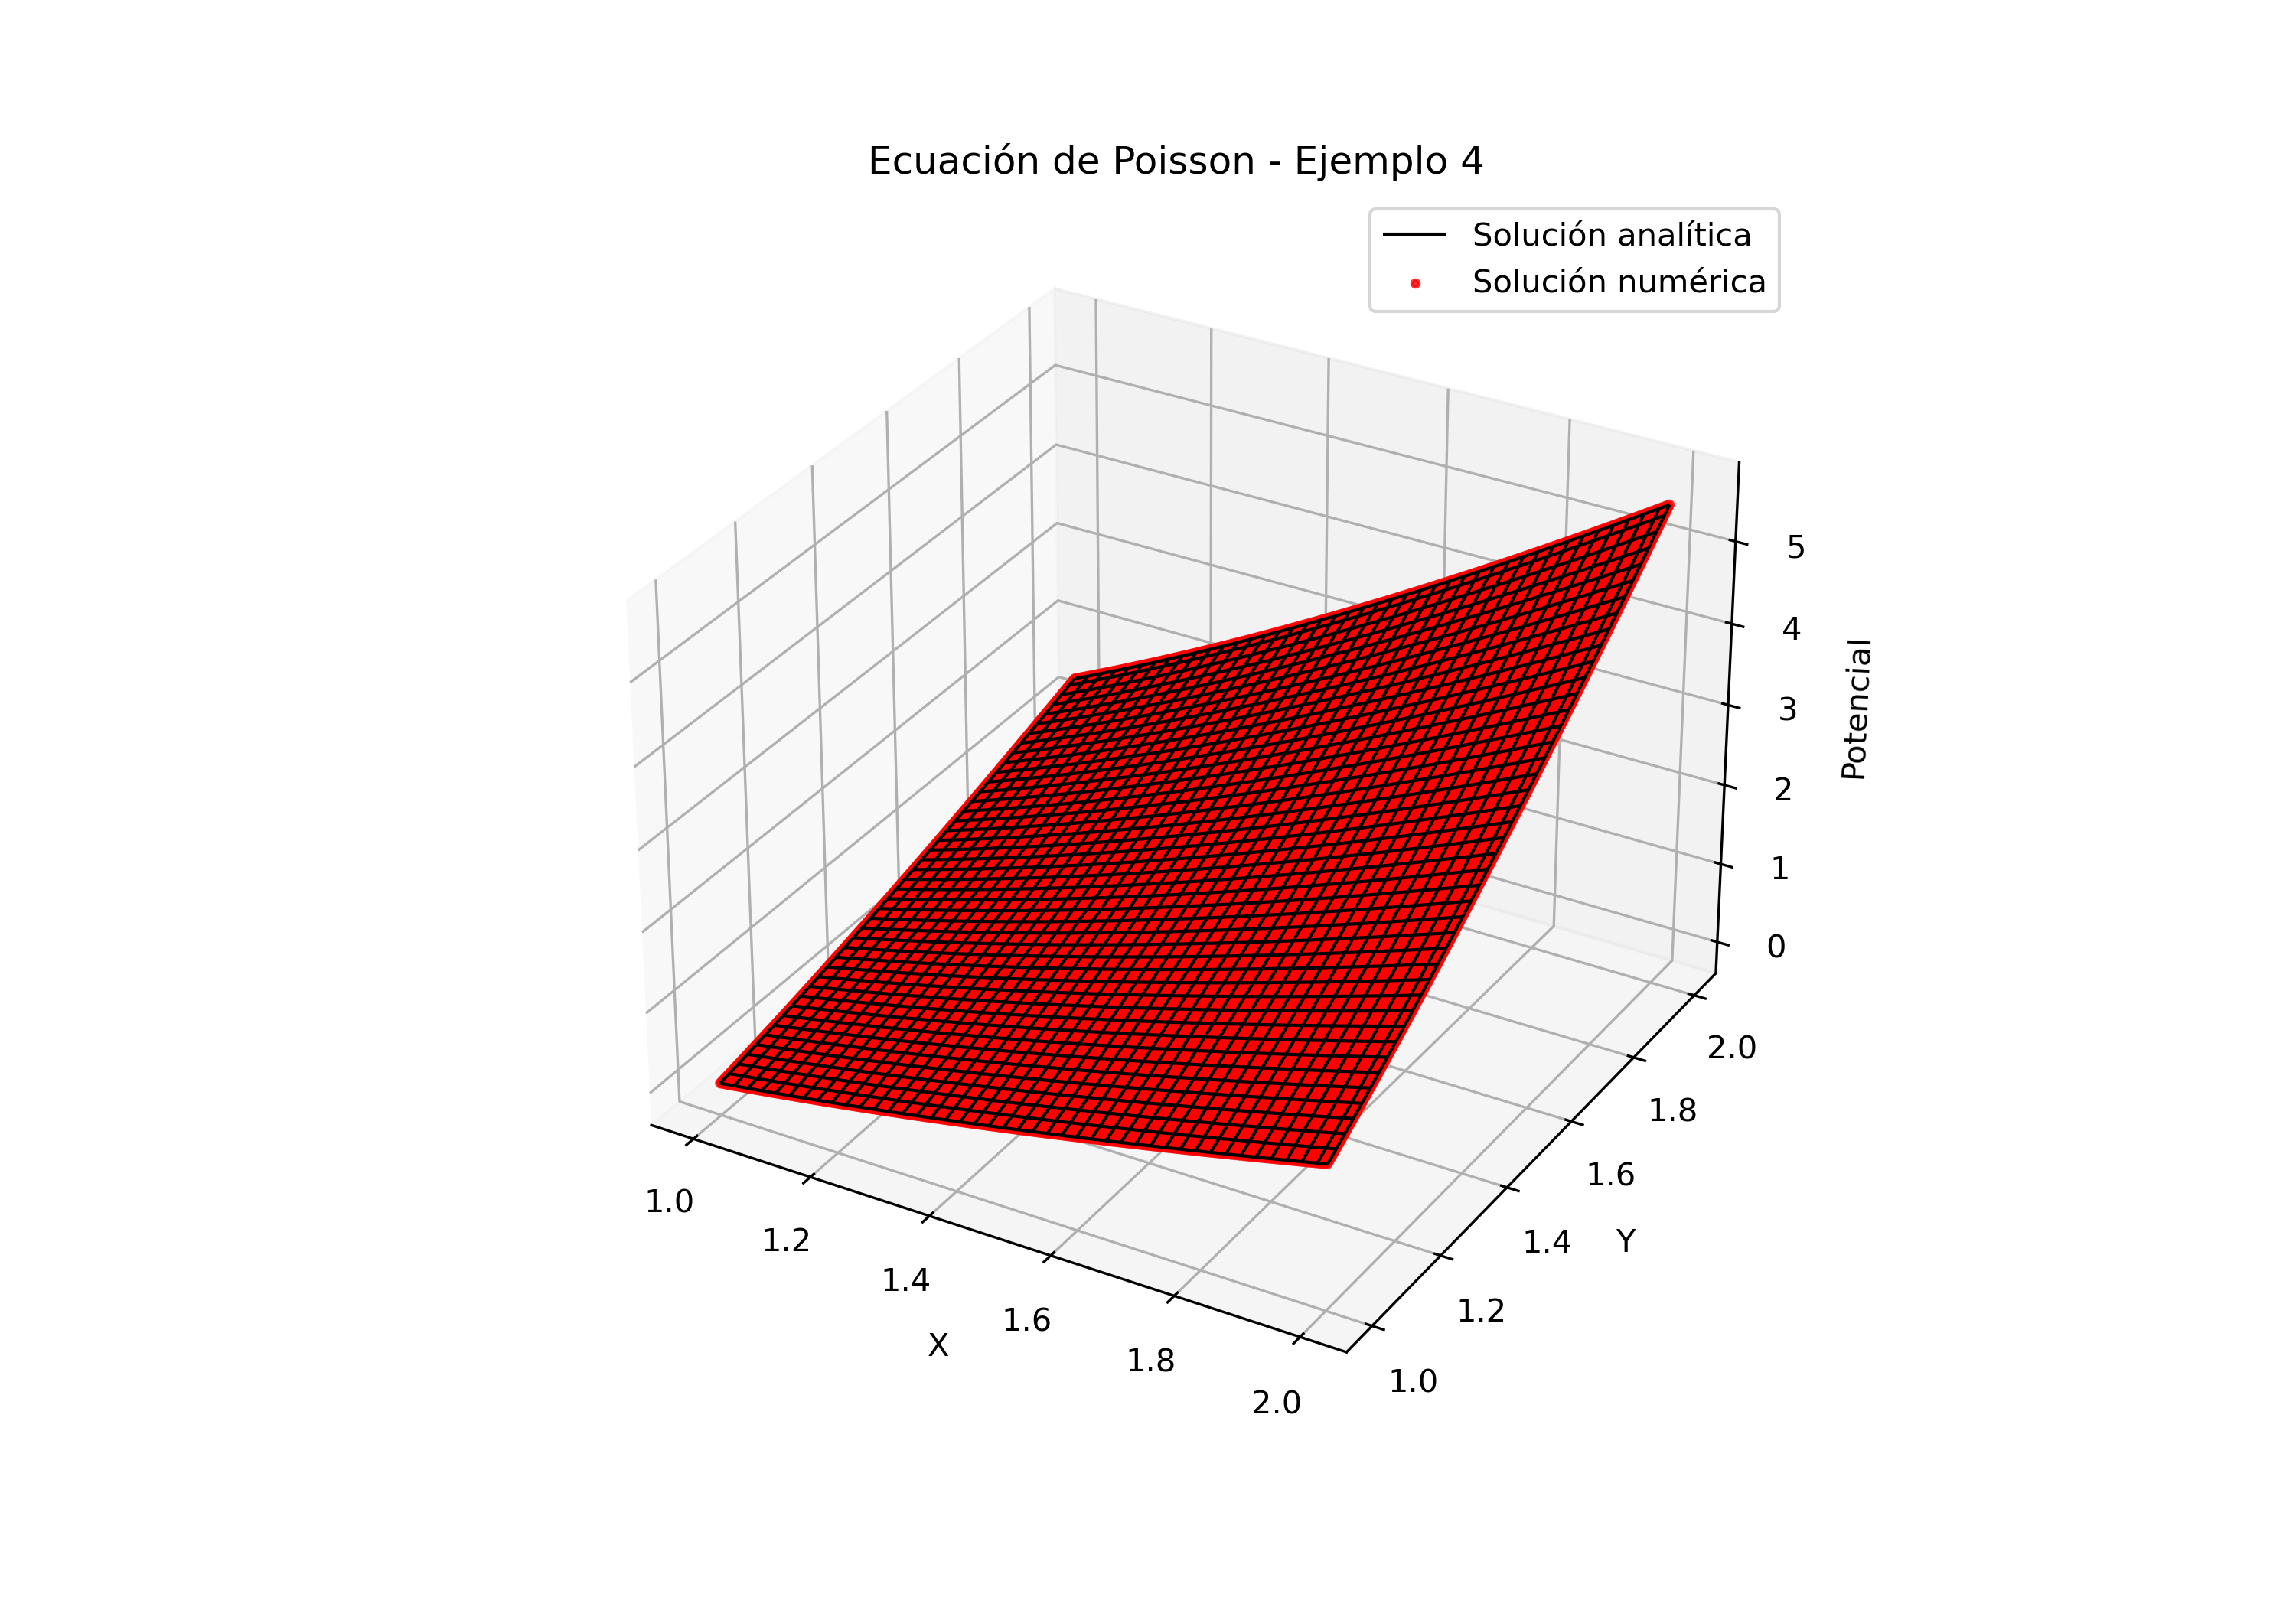
\includegraphics[width=0.8\textwidth]{imag/solucion_atomic_Ej4.png}
    \caption{Ejemplo 4 resuelto con \texttt{atomic}.}
\end{figure}
\begin{figure}[H]
    \centering
    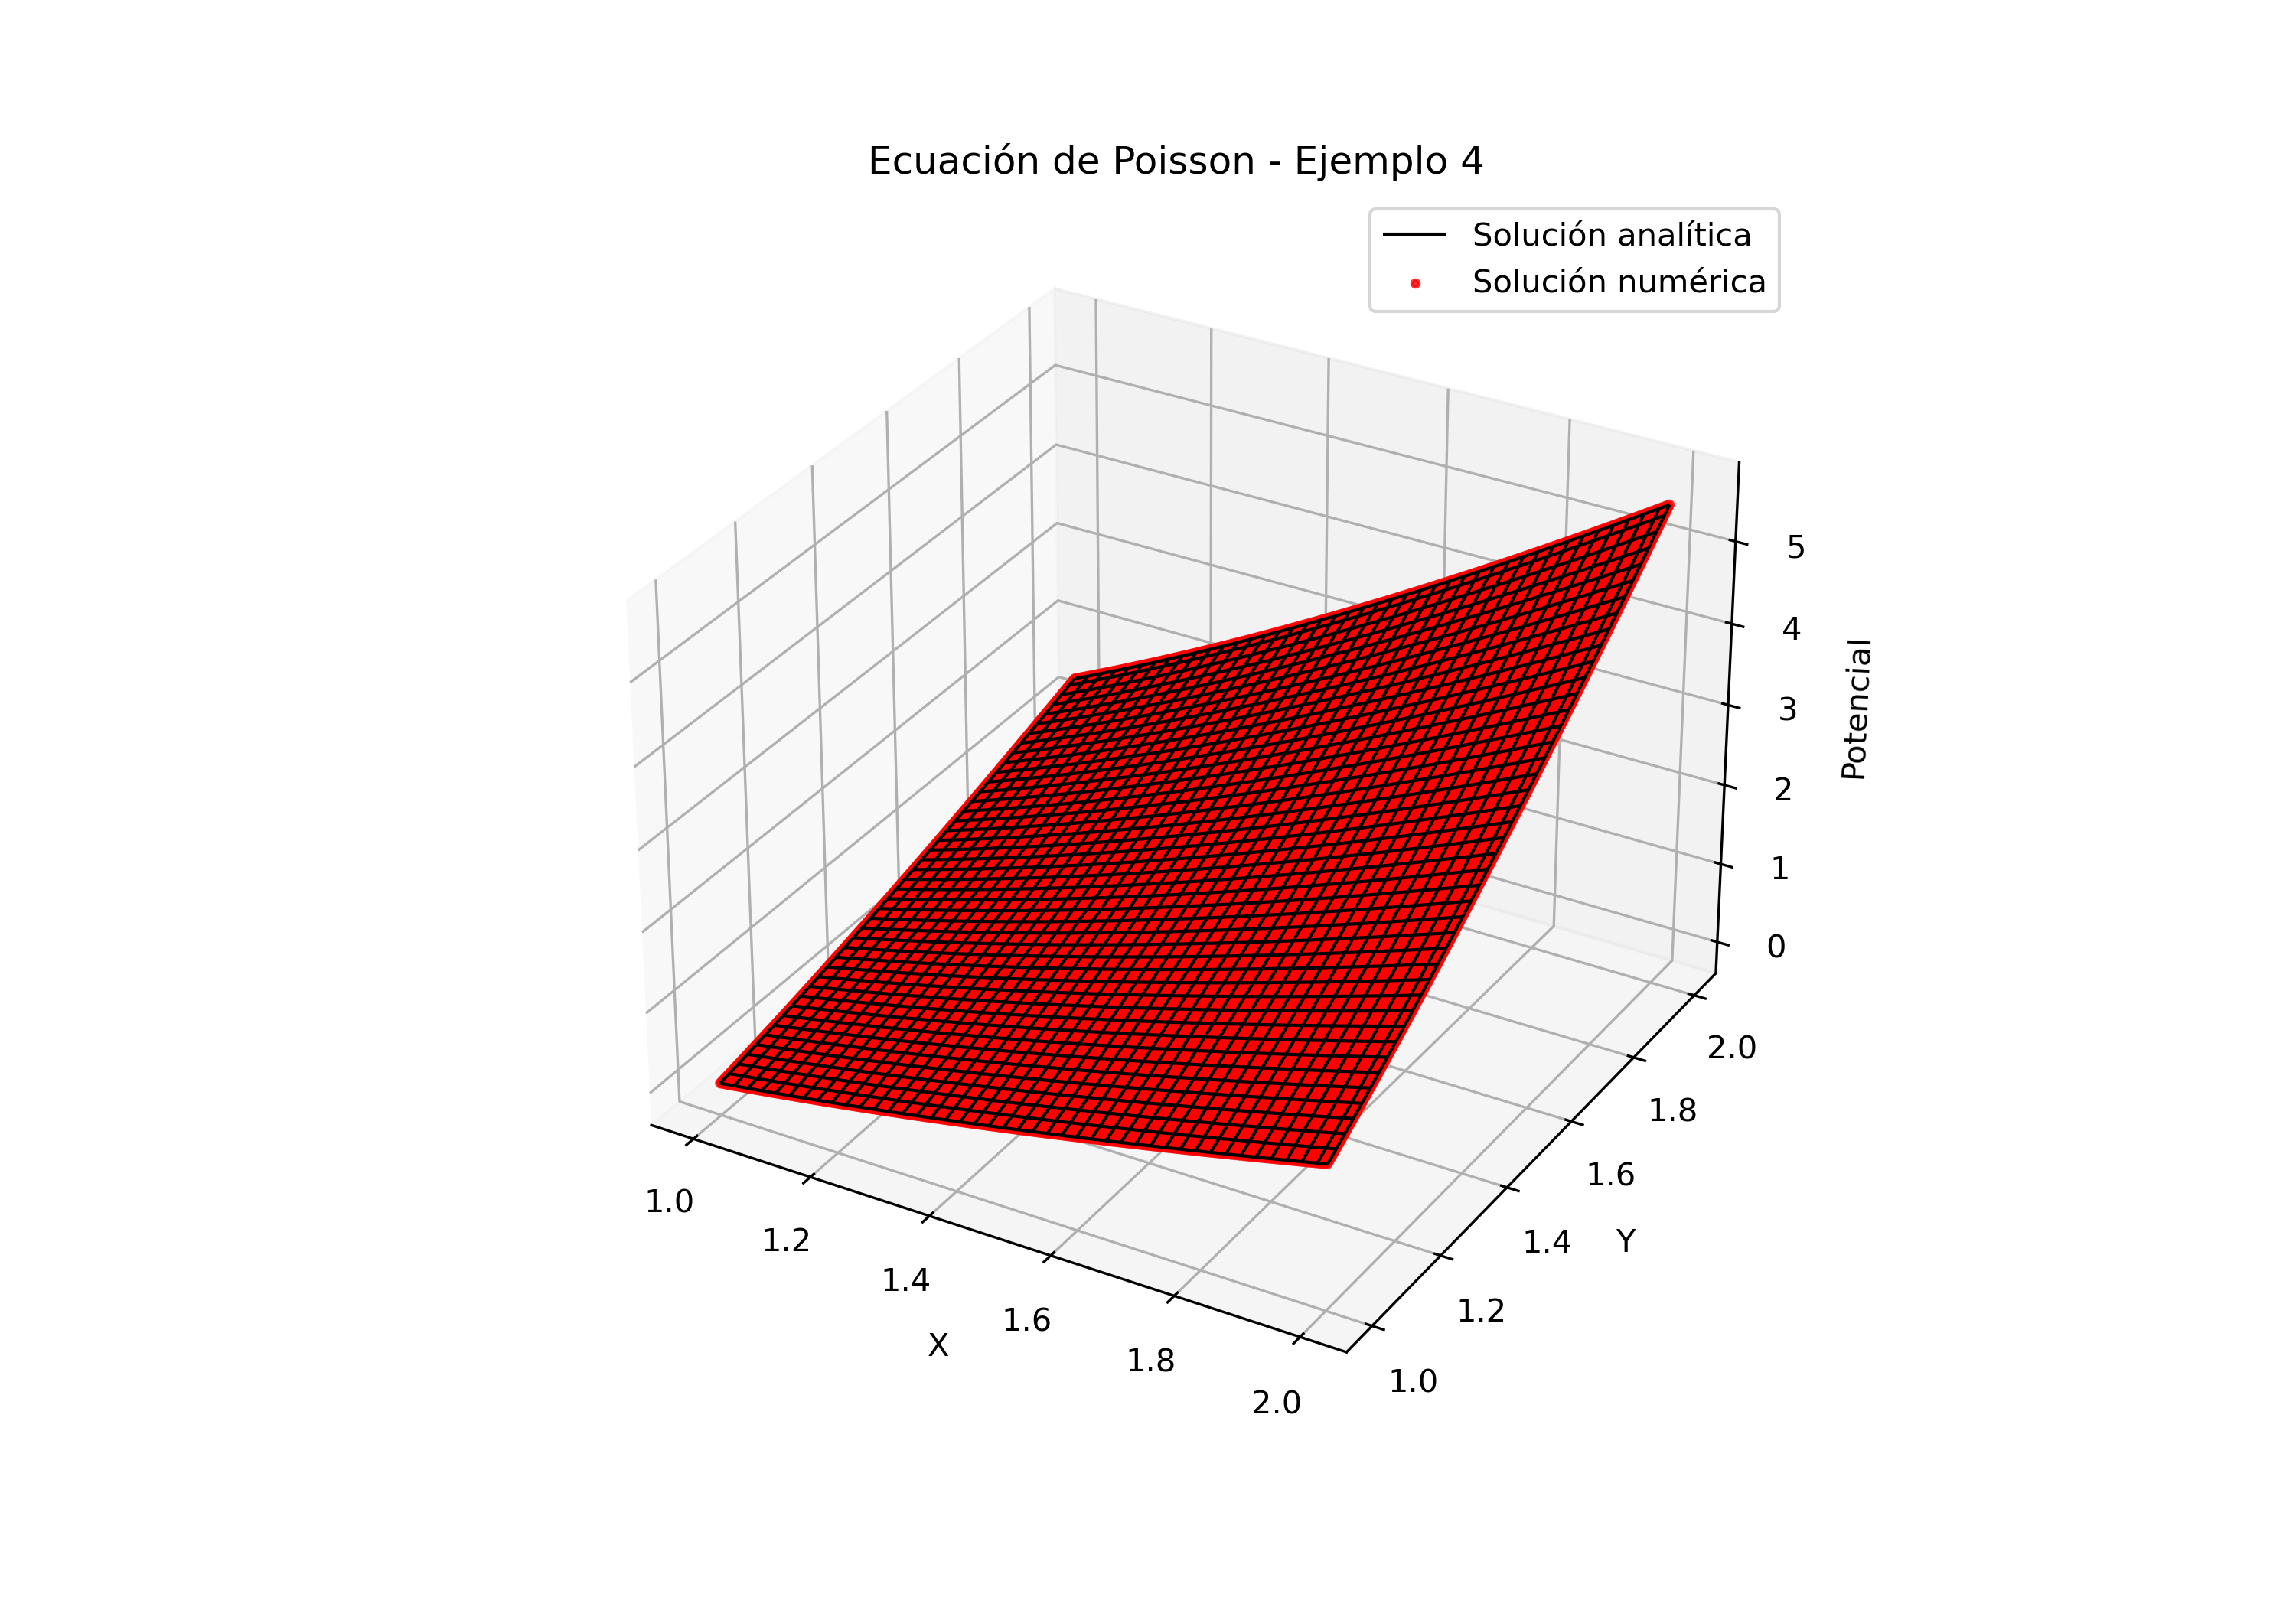
\includegraphics[width=0.8\textwidth]{imag/solucion_task_Ej4.png}
    \caption{Ejemplo 4 resuelto con \texttt{task}.}
\end{figure}

\section{Análisis de Rendimiento y Escalabilidad en Clúster}

Para evaluar la eficiencia de las directivas OpenMP empleadas, se llevó a cabo un experimento computacional en el clúster ejecutando los cinco códigos iterativos (Serial, Parallel For, Critical, Atomic y Task) sobre dos tamaños de malla distintos: $N=50$ y $N=250$. Se varió el número de hilos disponibles entre 12, 24, 48 y 64.

Los resultados arrojaron métricas de alto valor analítico que ilustran los límites del modelo de memoria compartida frente a la granularidad del problema.

\subsection{Caso 1: Malla Pequeña ($50 \times 50$)}
En la malla de baja resolución ($50 \times 50$), el algoritmo secuencial completó la simulación en apenas \textbf{0.193 segundos}. 

Al introducir paralelismo, se observó un fenómeno de \textbf{escalabilidad negativa extrema}. Con 12 hilos, el tiempo subió a $\sim$0.58 segundos; con 64 hilos, el tiempo ascendió a $\sim$3.5 segundos para las versiones atómicas/críticas, y superó los 5 segundos en la versión \texttt{task}. 

Este comportamiento demuestra que para matrices pequeñas, la carga computacional distribuida a cada hilo es despreciable frente al \textit{overhead} (costo administrativo) del sistema. El procesador invierte la vasta mayoría del tiempo instanciando hilos, gestionando la barrera de sincronización implícita de los bloques \texttt{for}, y encolando tareas, en lugar de realizar cálculos flotantes efectivos.

\begin{figure}[H]
    \centering
    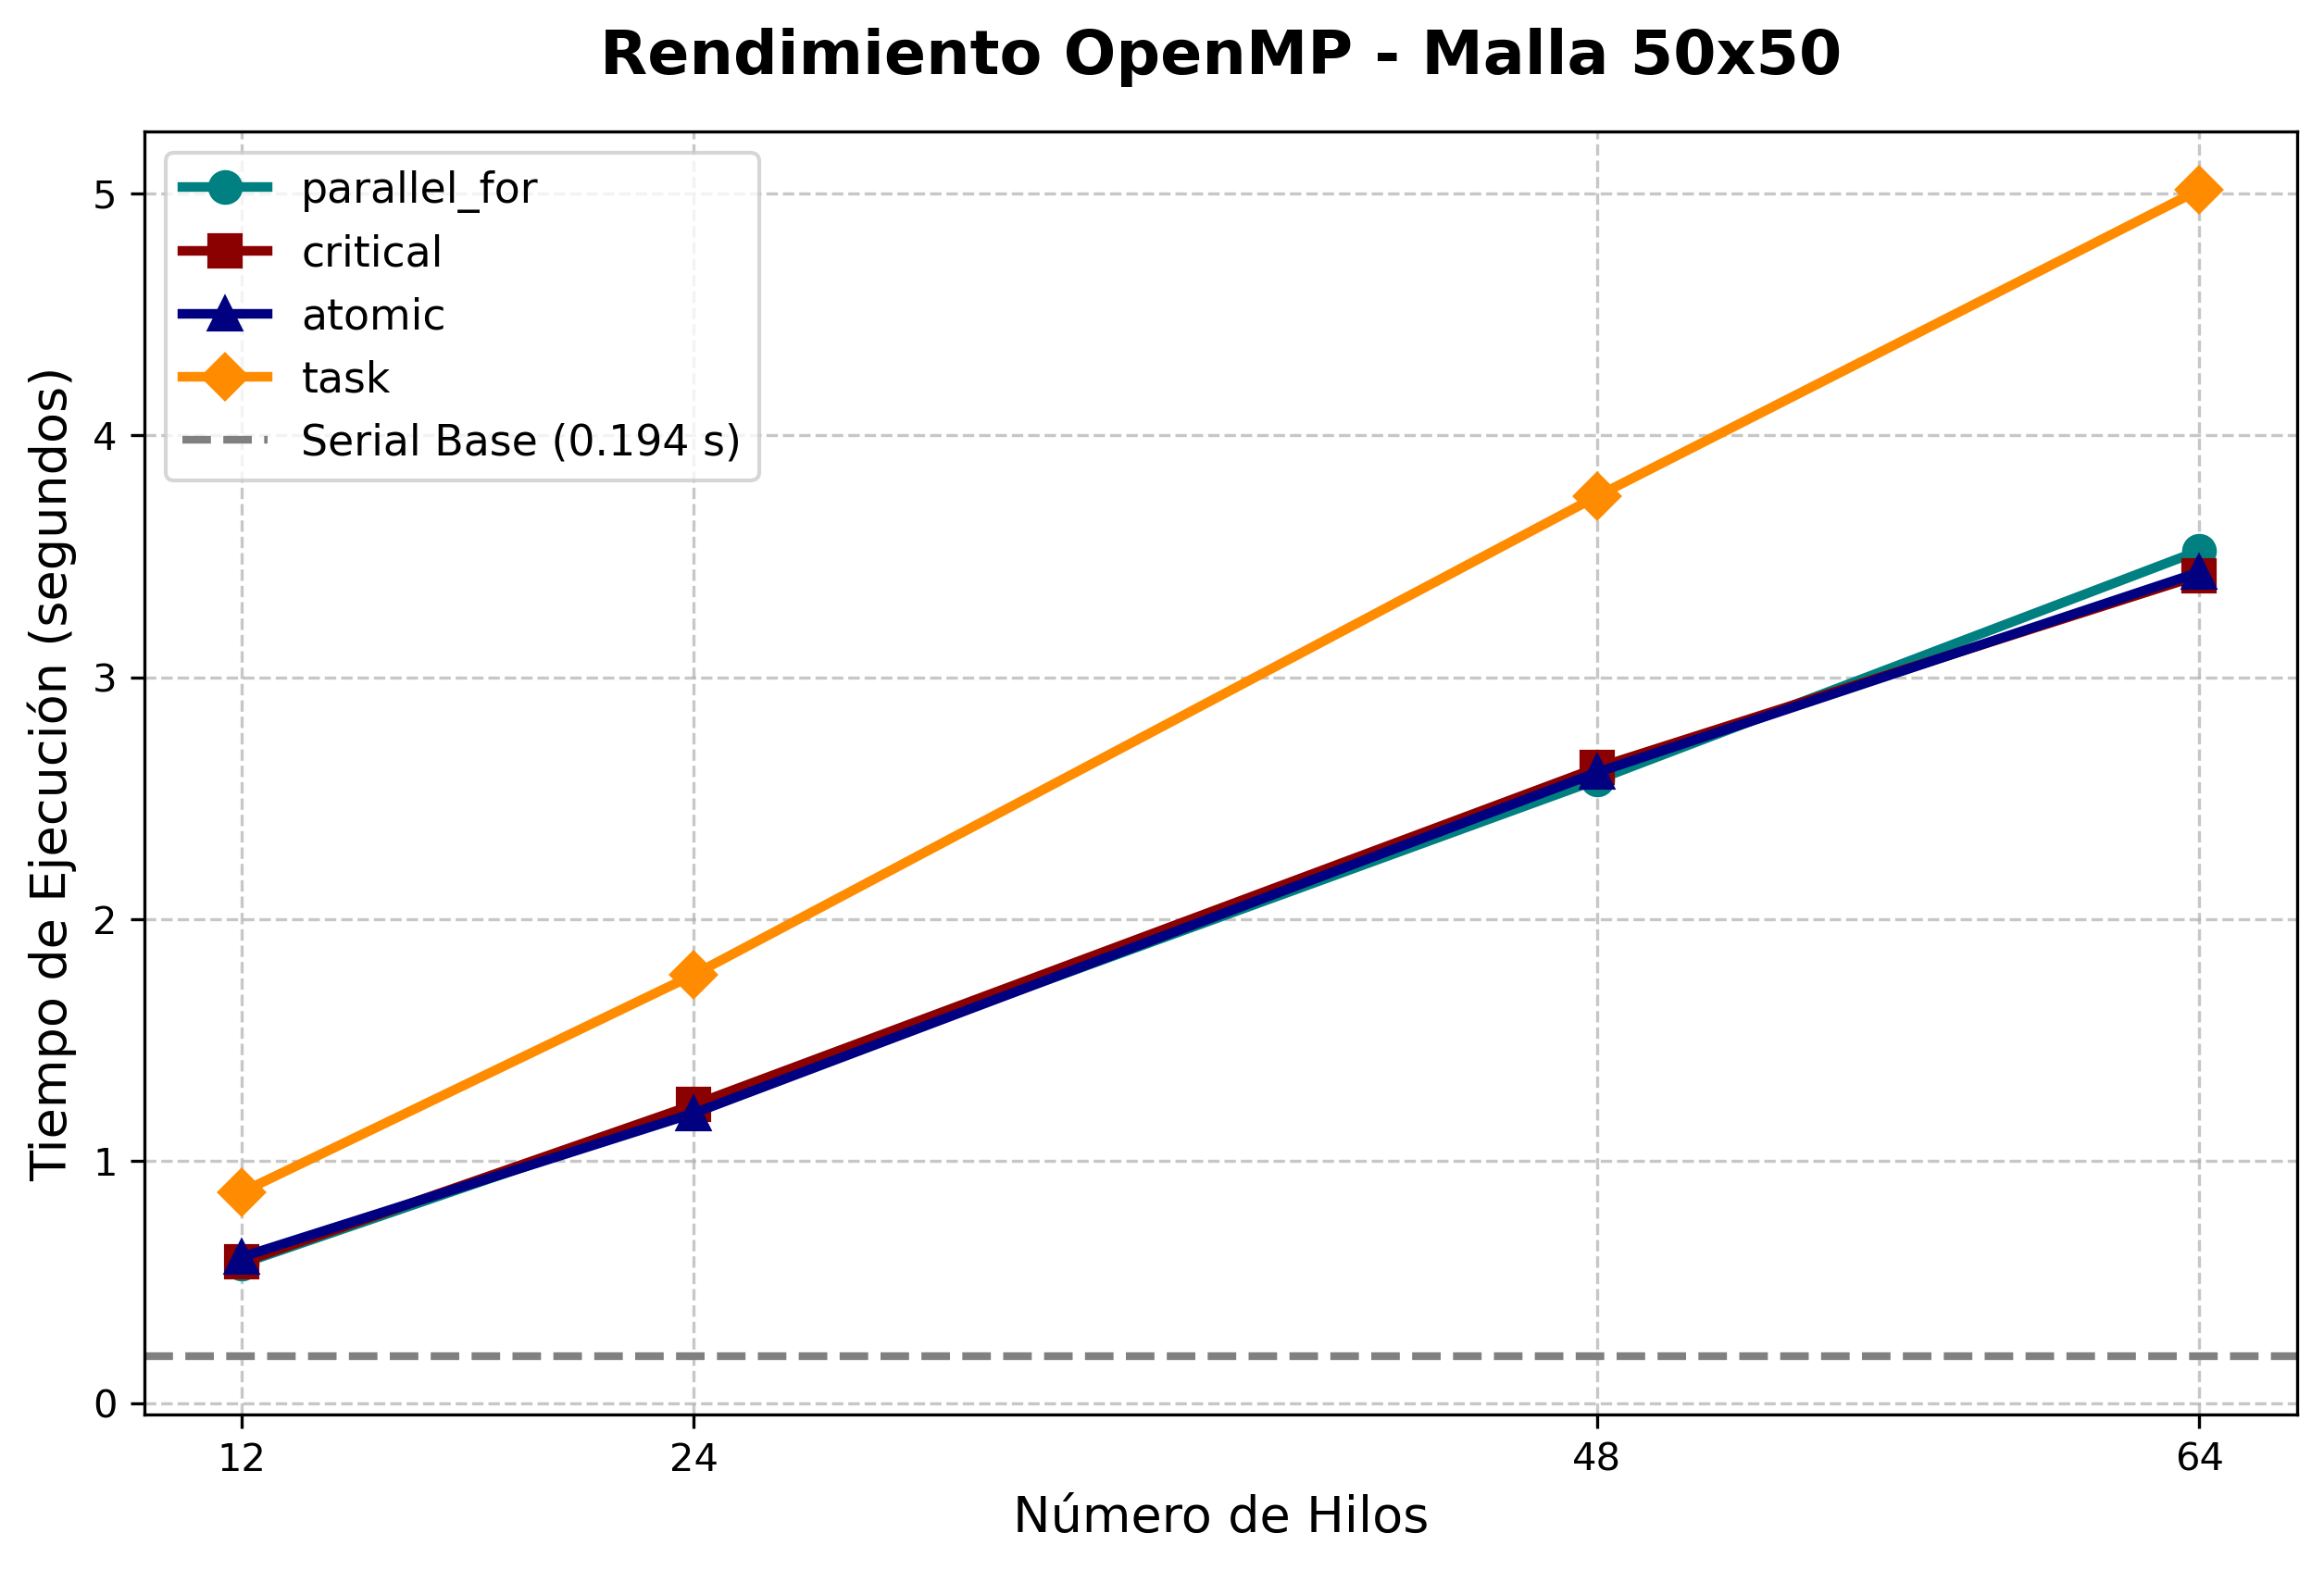
\includegraphics[width=0.8\textwidth]{imag/Rendimiento_Tiempos_N50.png}
    \caption{Tiempos de ejecución para $N=50$. La línea punteada indica el tiempo serial; todos los métodos paralelos son más lentos debido al \textit{overhead} de OpenMP.}
\end{figure}

\subsection{Caso 2: Malla Mediana ($250 \times 250$)}
Al aumentar la grilla geométrica a $250 \times 250$, la carga de cálculo crece exponencialmente. El algoritmo secuencial tardó \textbf{88.11 segundos} en converger.

Al desplegar 12 hilos, el tiempo colapsó dramáticamente a $\sim$\textbf{32.12 segundos} (en las versiones \texttt{parallel for} y \texttt{critical}), logrando un \textit{speedup} de $\sim$2.74x. Esto confirma que el paralelismo es altamente efectivo cuando hay suficiente volumen de datos para amortizar el costo de sincronización.

Sin embargo, al escalar a 24 hilos, se identificó un \textbf{cuello de botella de memoria compartida}. El tiempo de ejecución se degradó, subiendo de 32 segundos a \textbf{52.92 segundos} en la versión \texttt{parallel for}, y a 43.87 segundos en \texttt{critical}. Este fenómeno sugiere dos posibles causas ligadas a la arquitectura del clúster:
\begin{enumerate}
    \item \textbf{Falsa Compartición (\textit{False Sharing}):} Los hilos procesan filas contiguas de la matriz, provocando que múltiples núcleos invaliden constantemente las líneas de caché de nivel 1 (L1) y nivel 2 (L2) de los demás, destruyendo el ancho de banda.
    \item \textbf{Saturación del Bus de Memoria:} Aunque el número de núcleos aumente, el canal físico hacia la memoria RAM es el mismo. A partir de 12 hilos, las peticiones de lectura/escritura compiten simultáneamente bloqueando el acceso de los demás procesos.
\end{enumerate}

\begin{figure}[H]
    \centering
    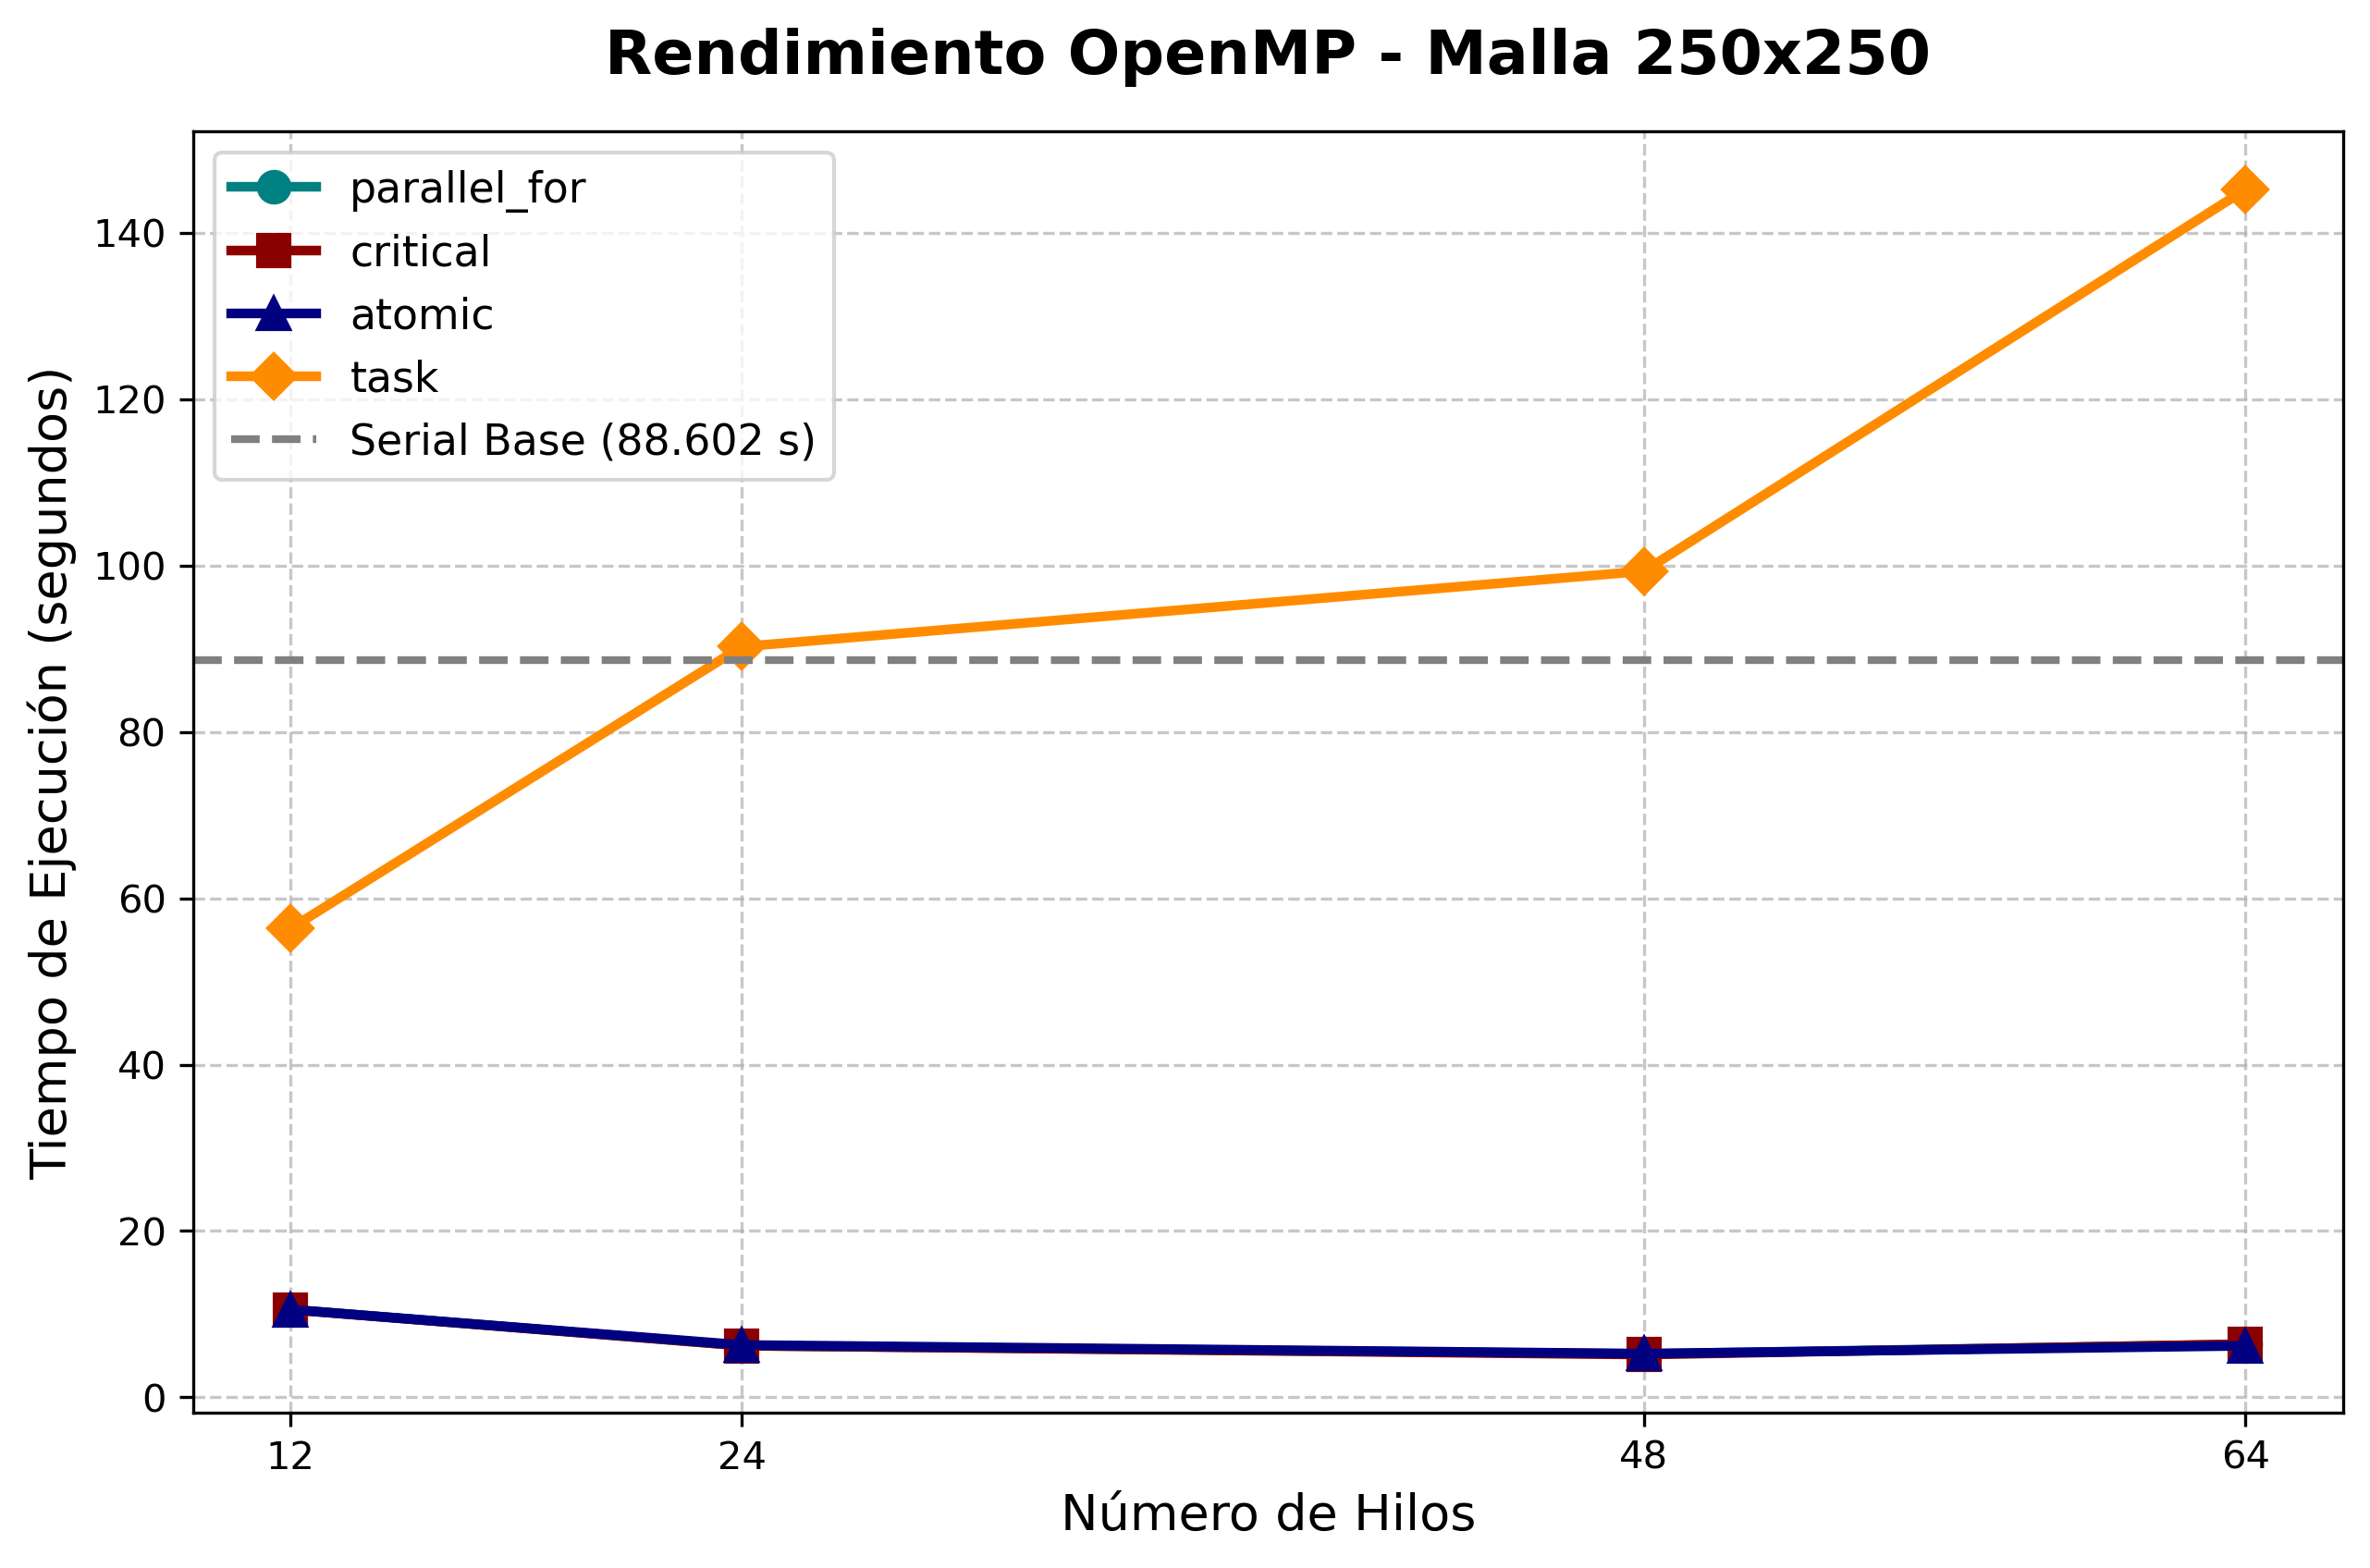
\includegraphics[width=0.8\textwidth]{imag/Rendimiento_Tiempos_N250.png}
    \caption{Tiempos de ejecución para $N=250$. Se observa un \textit{speedup} considerable con 12 hilos, seguido de una degradación por contención de memoria al saltar a 24 hilos.}
\end{figure}

\subsection{Comparativa de Directivas}
En cuanto a las directivas evaluadas, se concluye lo siguiente:
\begin{itemize}
    \item \texttt{parallel for collapse(2)} demostró ser el mecanismo más limpio y eficiente, equilibrando la carga al máximo.
    \item \texttt{atomic} y \texttt{critical} no mostraron diferencias sustanciales en tiempo debido a que la variable compartida (\texttt{iterations}) se actualiza en un bloque externo al bucle pesado.
    \item La directiva \texttt{task} arrojó consistentemente los peores tiempos (\textit{overhead} máximo), demostrando que la gestión de colas de tareas asíncronas no es la estrategia adecuada para problemas fuertemente estructurados y densos como las mallas de diferencias finitas.
\end{itemize}

\subsection{Caso 3: Malla Masiva ($1000 \times 1000$) y Límite Arquitectónico}

El verdadero potencial y las limitaciones de la arquitectura de memoria compartida se hacen evidentes al escalar el dominio a una malla densa de $1000 \times 1000$ celdas (un millón de puntos evaluados por iteración). 

Bajo estas condiciones de estrés, el algoritmo \textbf{secuencial} base requirió \textbf{18,878.71 segundos} (aproximadamente 5.24 horas) para alcanzar la convergencia de la simulación. Al aplicar el paralelismo, los resultados divergen drásticamente dependiendo de la directiva utilizada:

\begin{itemize}
    \item \textbf{Eficiencia de \texttt{parallel for}:} La directiva de paralelización de bucles con \texttt{collapse(2)} exhibió un escalamiento brillante, reduciendo el tiempo a \textbf{408.73 segundos} al emplear 64 hilos. Esto representa un \textit{speedup} (aceleración) de $\sim$\textbf{46.18x} respecto a la versión serial.
    
    \item \textbf{Penalización por Sincronización (\texttt{critical} y \texttt{atomic}):} Aunque a 12 y 24 hilos compiten estrechamente con el \texttt{parallel for}, al saturar el clúster con 48 y 64 hilos el rendimiento se degrada. Con 64 hilos, \texttt{critical} sube a 665.57s y \texttt{atomic} a 802.71s. Esta degradación se debe a la \textbf{contención extrema}: decenas de hilos intentando bloquear y actualizar una misma variable compartida (el contador de iteraciones o el cálculo del error máximo) en cada microsegundo, generando cuellos de botella en el bus de caché del procesador.
    
    \item \textbf{Sobrecarga de Tareas (\texttt{task}):} El enfoque orientado a tareas (\texttt{tasking}) resultó ser el menos eficiente para este problema matemático altamente estructurado. A 64 hilos, el tiempo ascendió a 2,906 segundos. La sobrecarga generada por el sistema en tiempo de ejecución de OpenMP para crear, encolar, gestionar dependencias y destruir millones de tareas asíncronas eclipsa las ventajas de repartir la carga.
\end{itemize}

\begin{figure}[H]
    \centering
    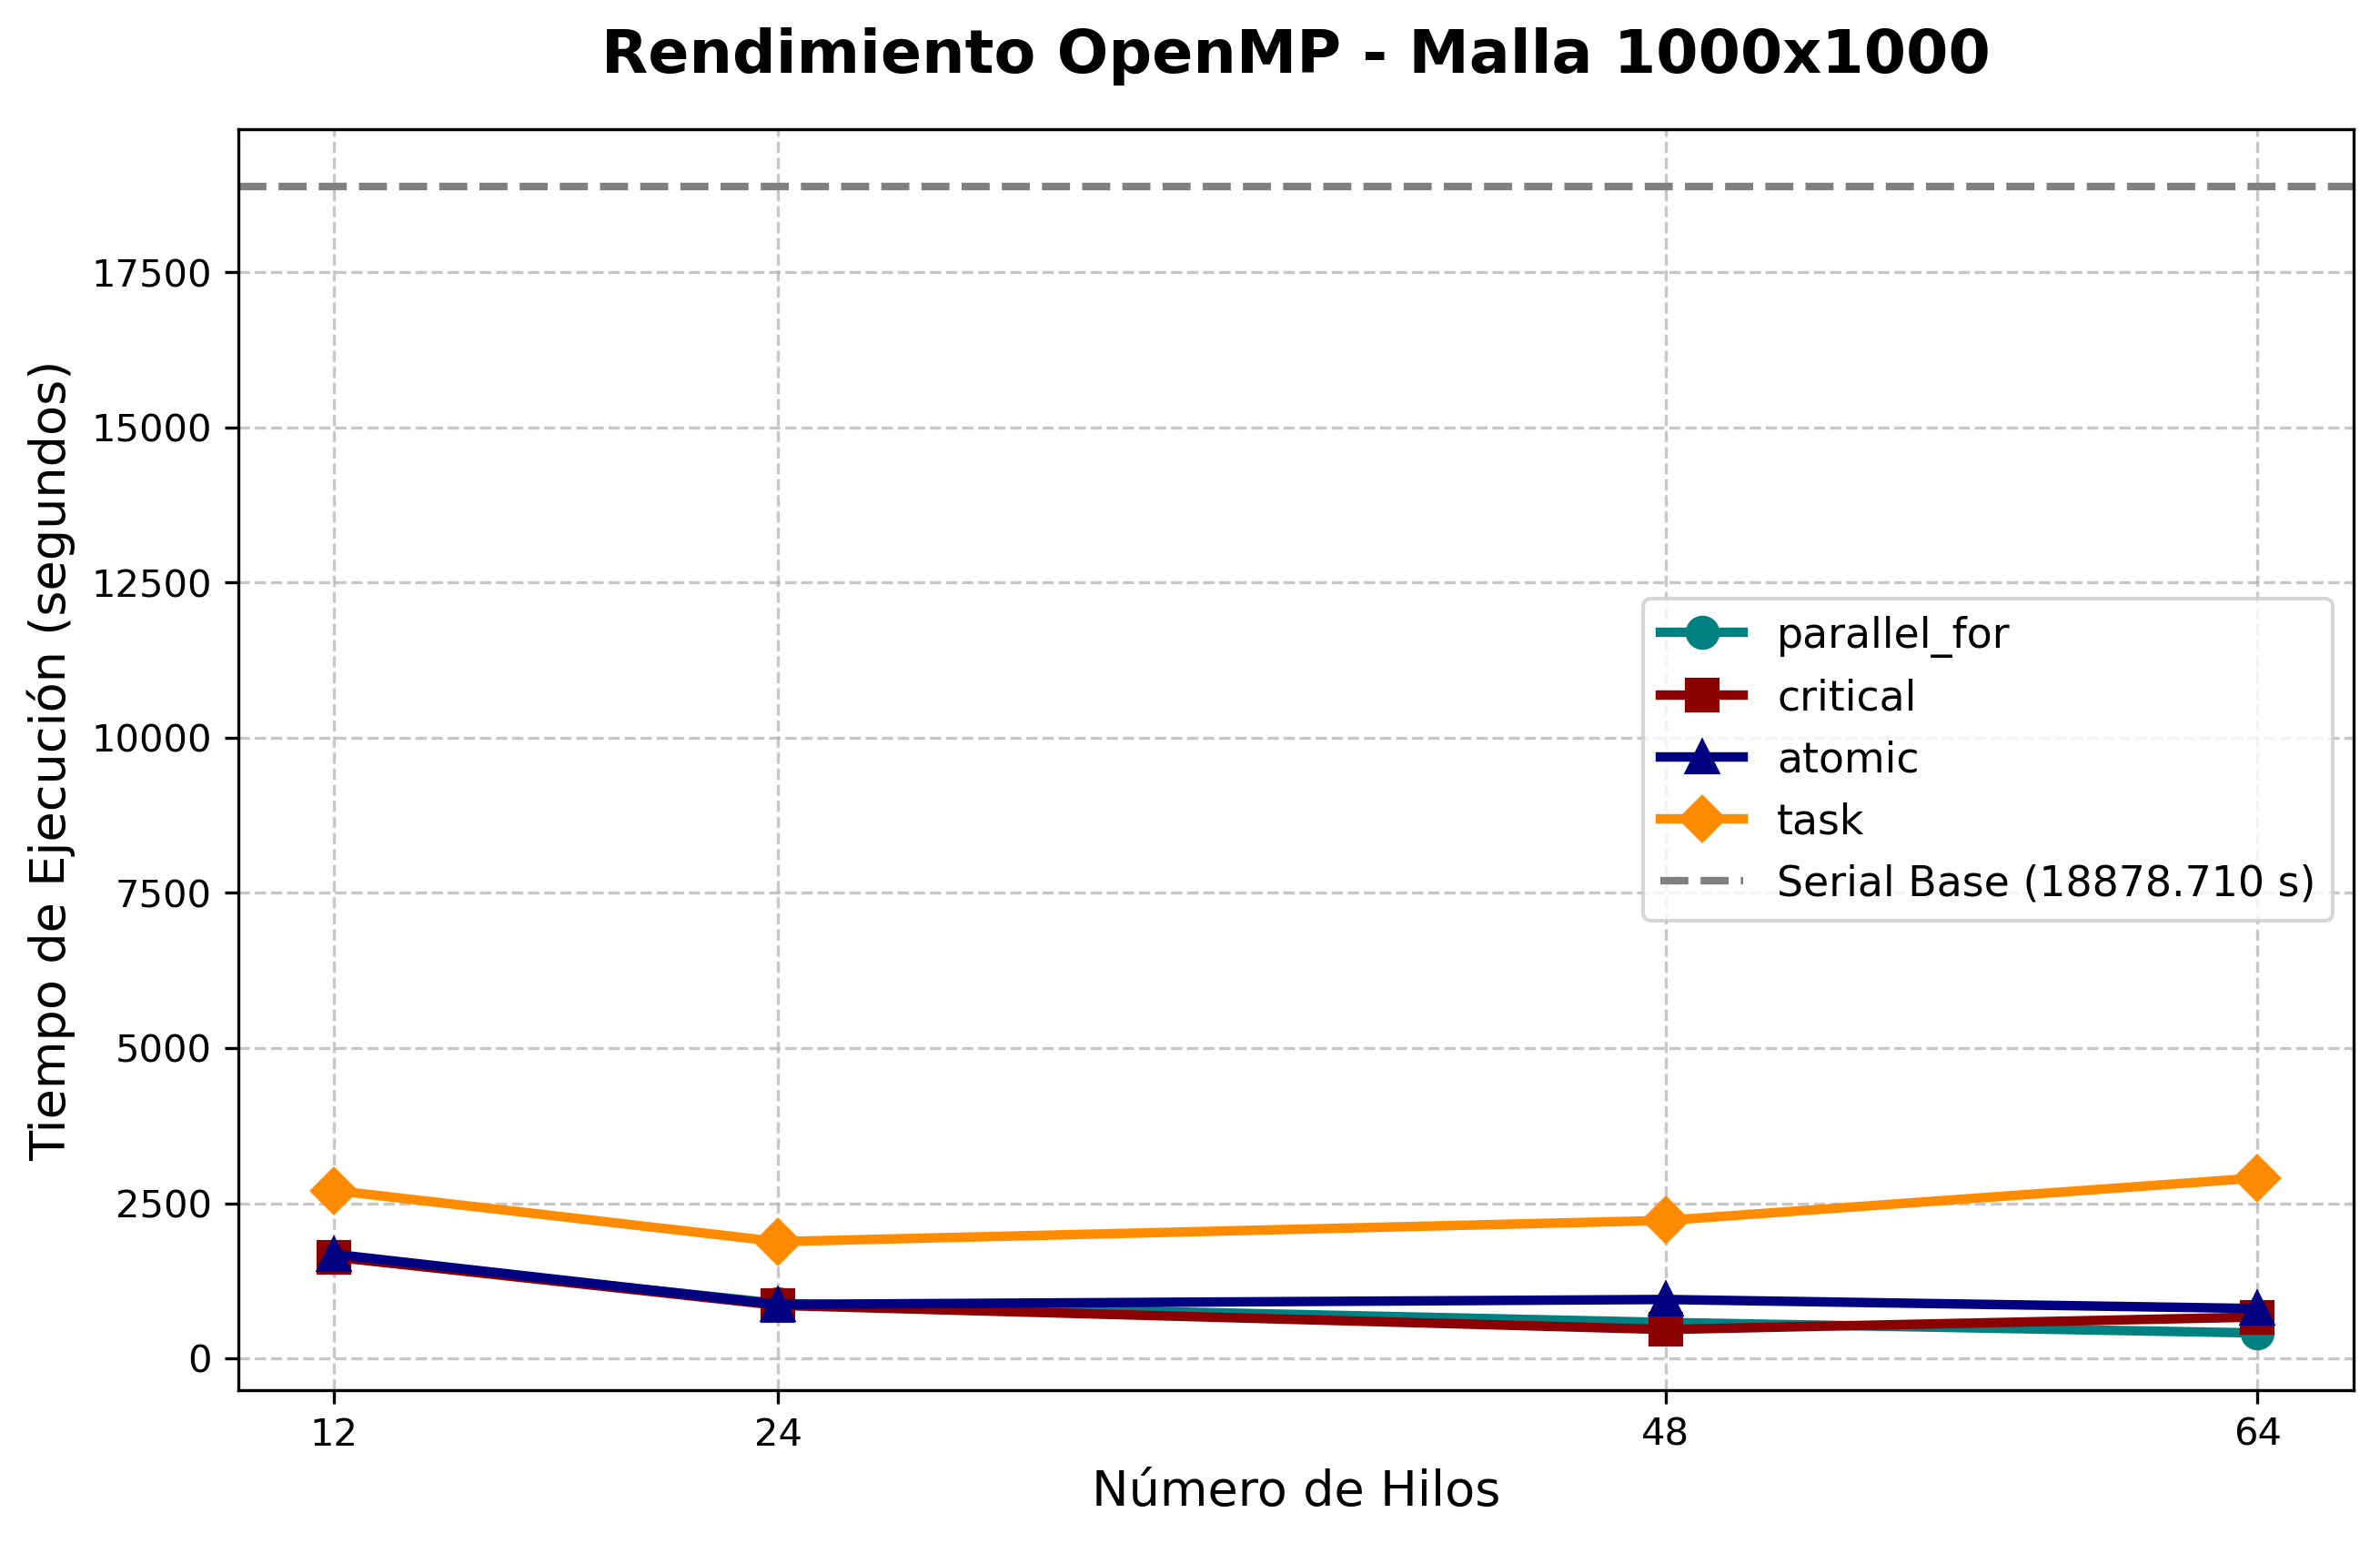
\includegraphics[width=0.8\textwidth]{imag/Rendimiento_Tiempos_N1000.png}
    \caption{Tiempos de ejecución para la malla masiva de $1000 \times 1000$. La línea punteada superior (fuera del cuadro principal) representa el tiempo serial de $\sim$5.2 horas. Se destaca la escalabilidad óptima del \texttt{parallel for} y el aumento de tiempos por contención en las estrategias de sincronización estricta a altos conteos de hilos.}
\end{figure}

\subsection{Visualización de la Escalabilidad Multihilo}

Las siguientes gráficas representan visualmente otros tiempos de ejecución obtenidos en el clúster. La línea segmentada horizontal establece la base de rendimiento secuencial, permitiendo identificar claramente a partir de qué punto el despliegue de hilos de OpenMP ofrece una ventaja competitiva frente al \textit{overhead} de sincronización.

\begin{figure}[H]
    \centering
    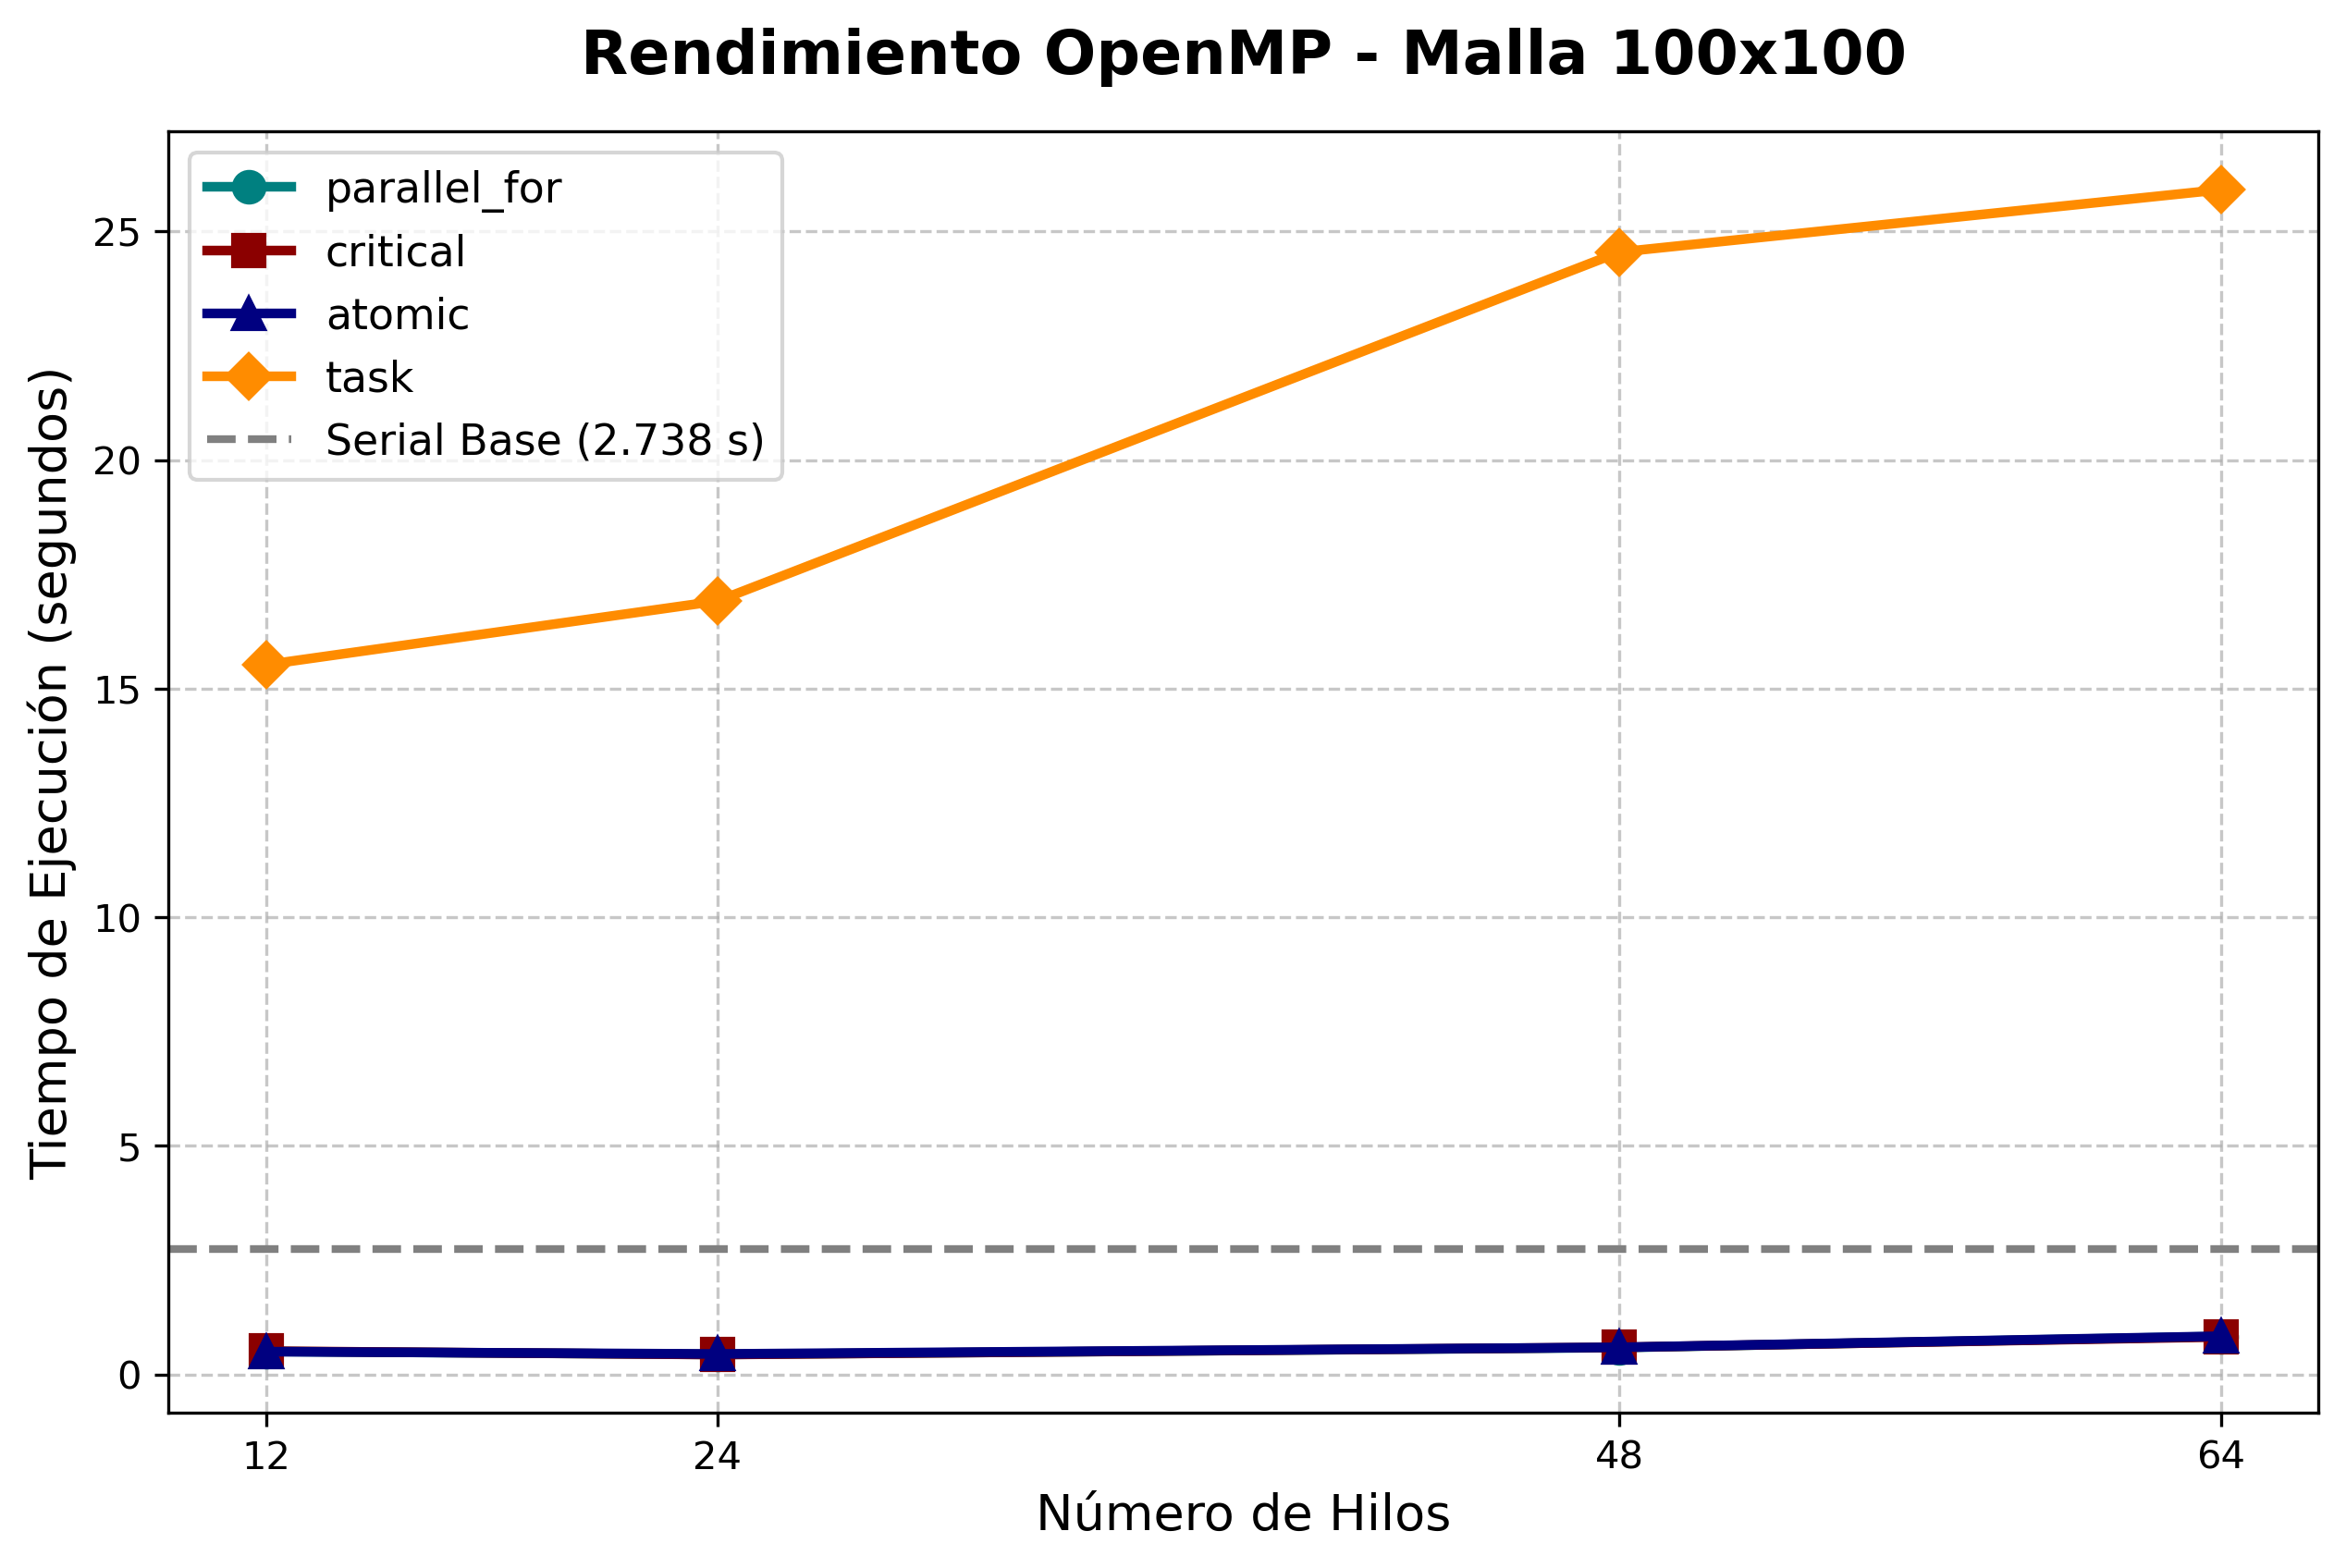
\includegraphics[width=0.8\textwidth]{imag/Rendimiento_Tiempos_N100.png}
    \caption{Tiempos de ejecución para la malla de $100 \times 100$. El tiempo secuencial es de 2.73 s. El punto de máxima eficiencia se alcanza con 24 hilos ($\sim 0.43$ s), tras lo cual la sobrecarga de comunicación penaliza el rendimiento. La directiva \texttt{task} resulta severamente ineficiente.}
\end{figure}

\begin{figure}[H]
    \centering
    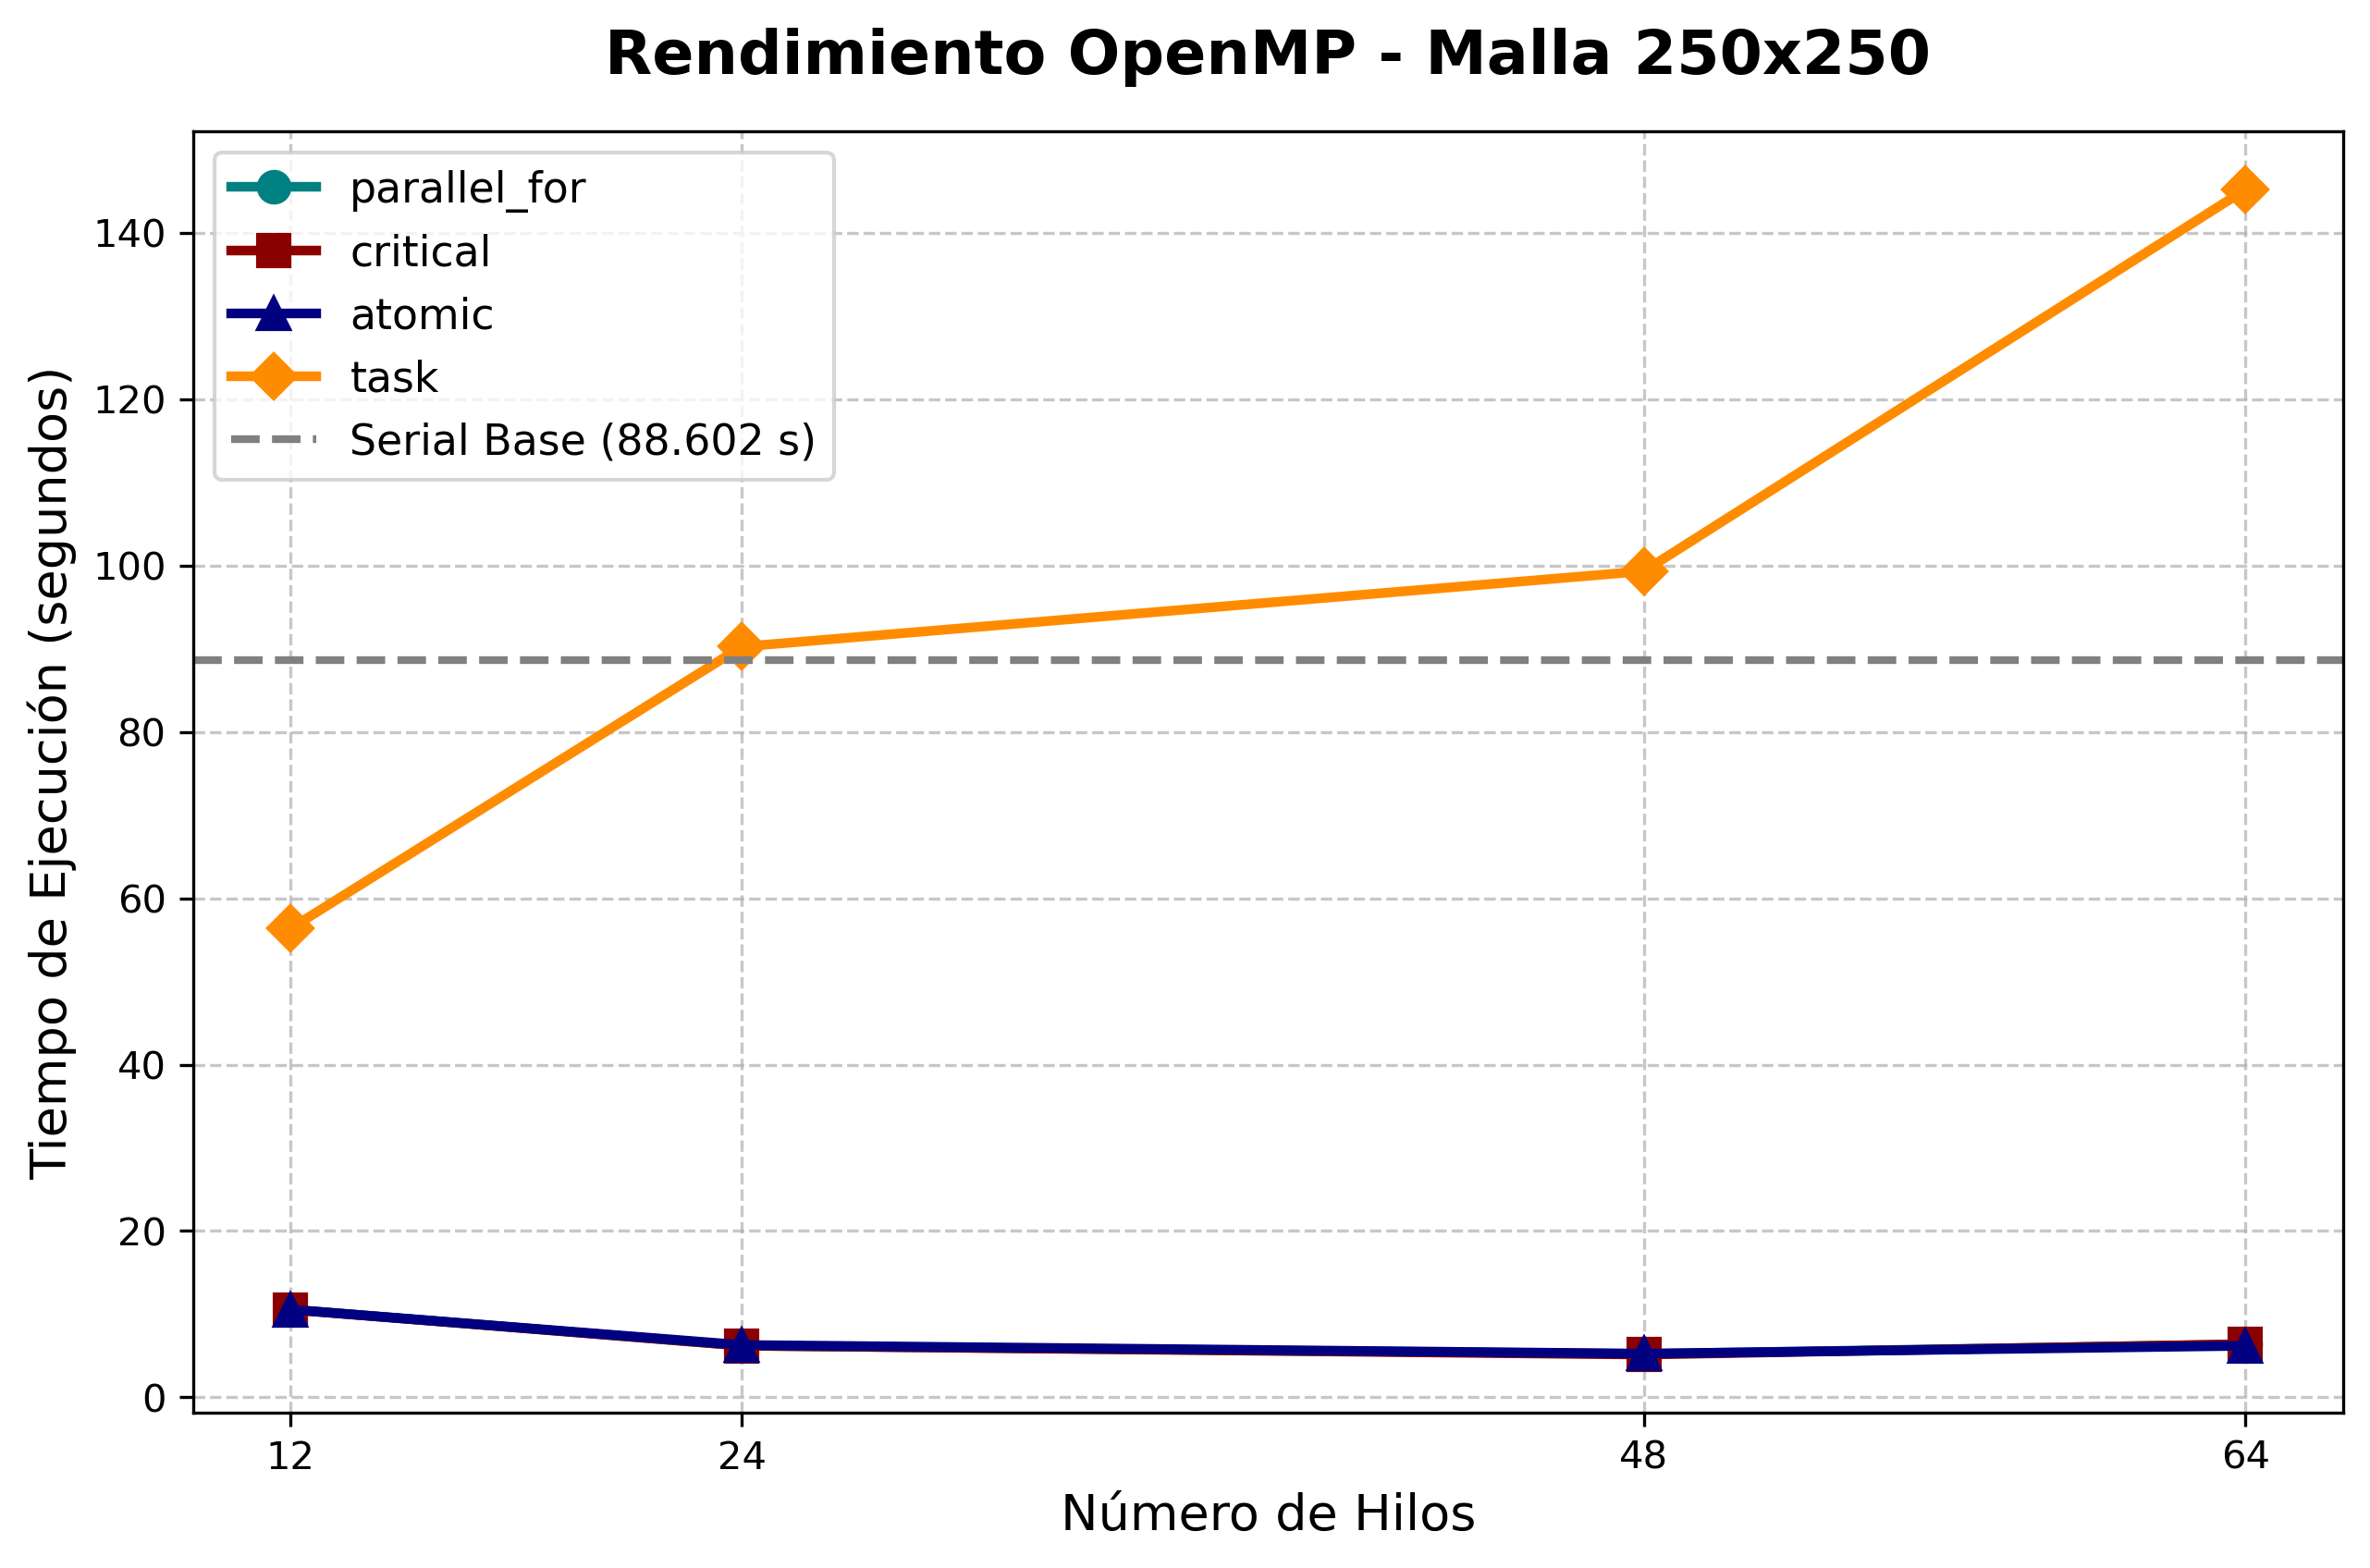
\includegraphics[width=0.8\textwidth]{imag/Rendimiento_Tiempos_N250.png}
    \caption{Tiempos de ejecución para la malla de $250 \times 250$. El tiempo base secuencial asciende a 88.6 s. El sistema encuentra su punto óptimo de aceleración alrededor de los 48 hilos ($\sim 5.1$ s), evidenciando un \textit{speedup} superior a 17x.}
\end{figure}

\begin{figure}[H]
    \centering
    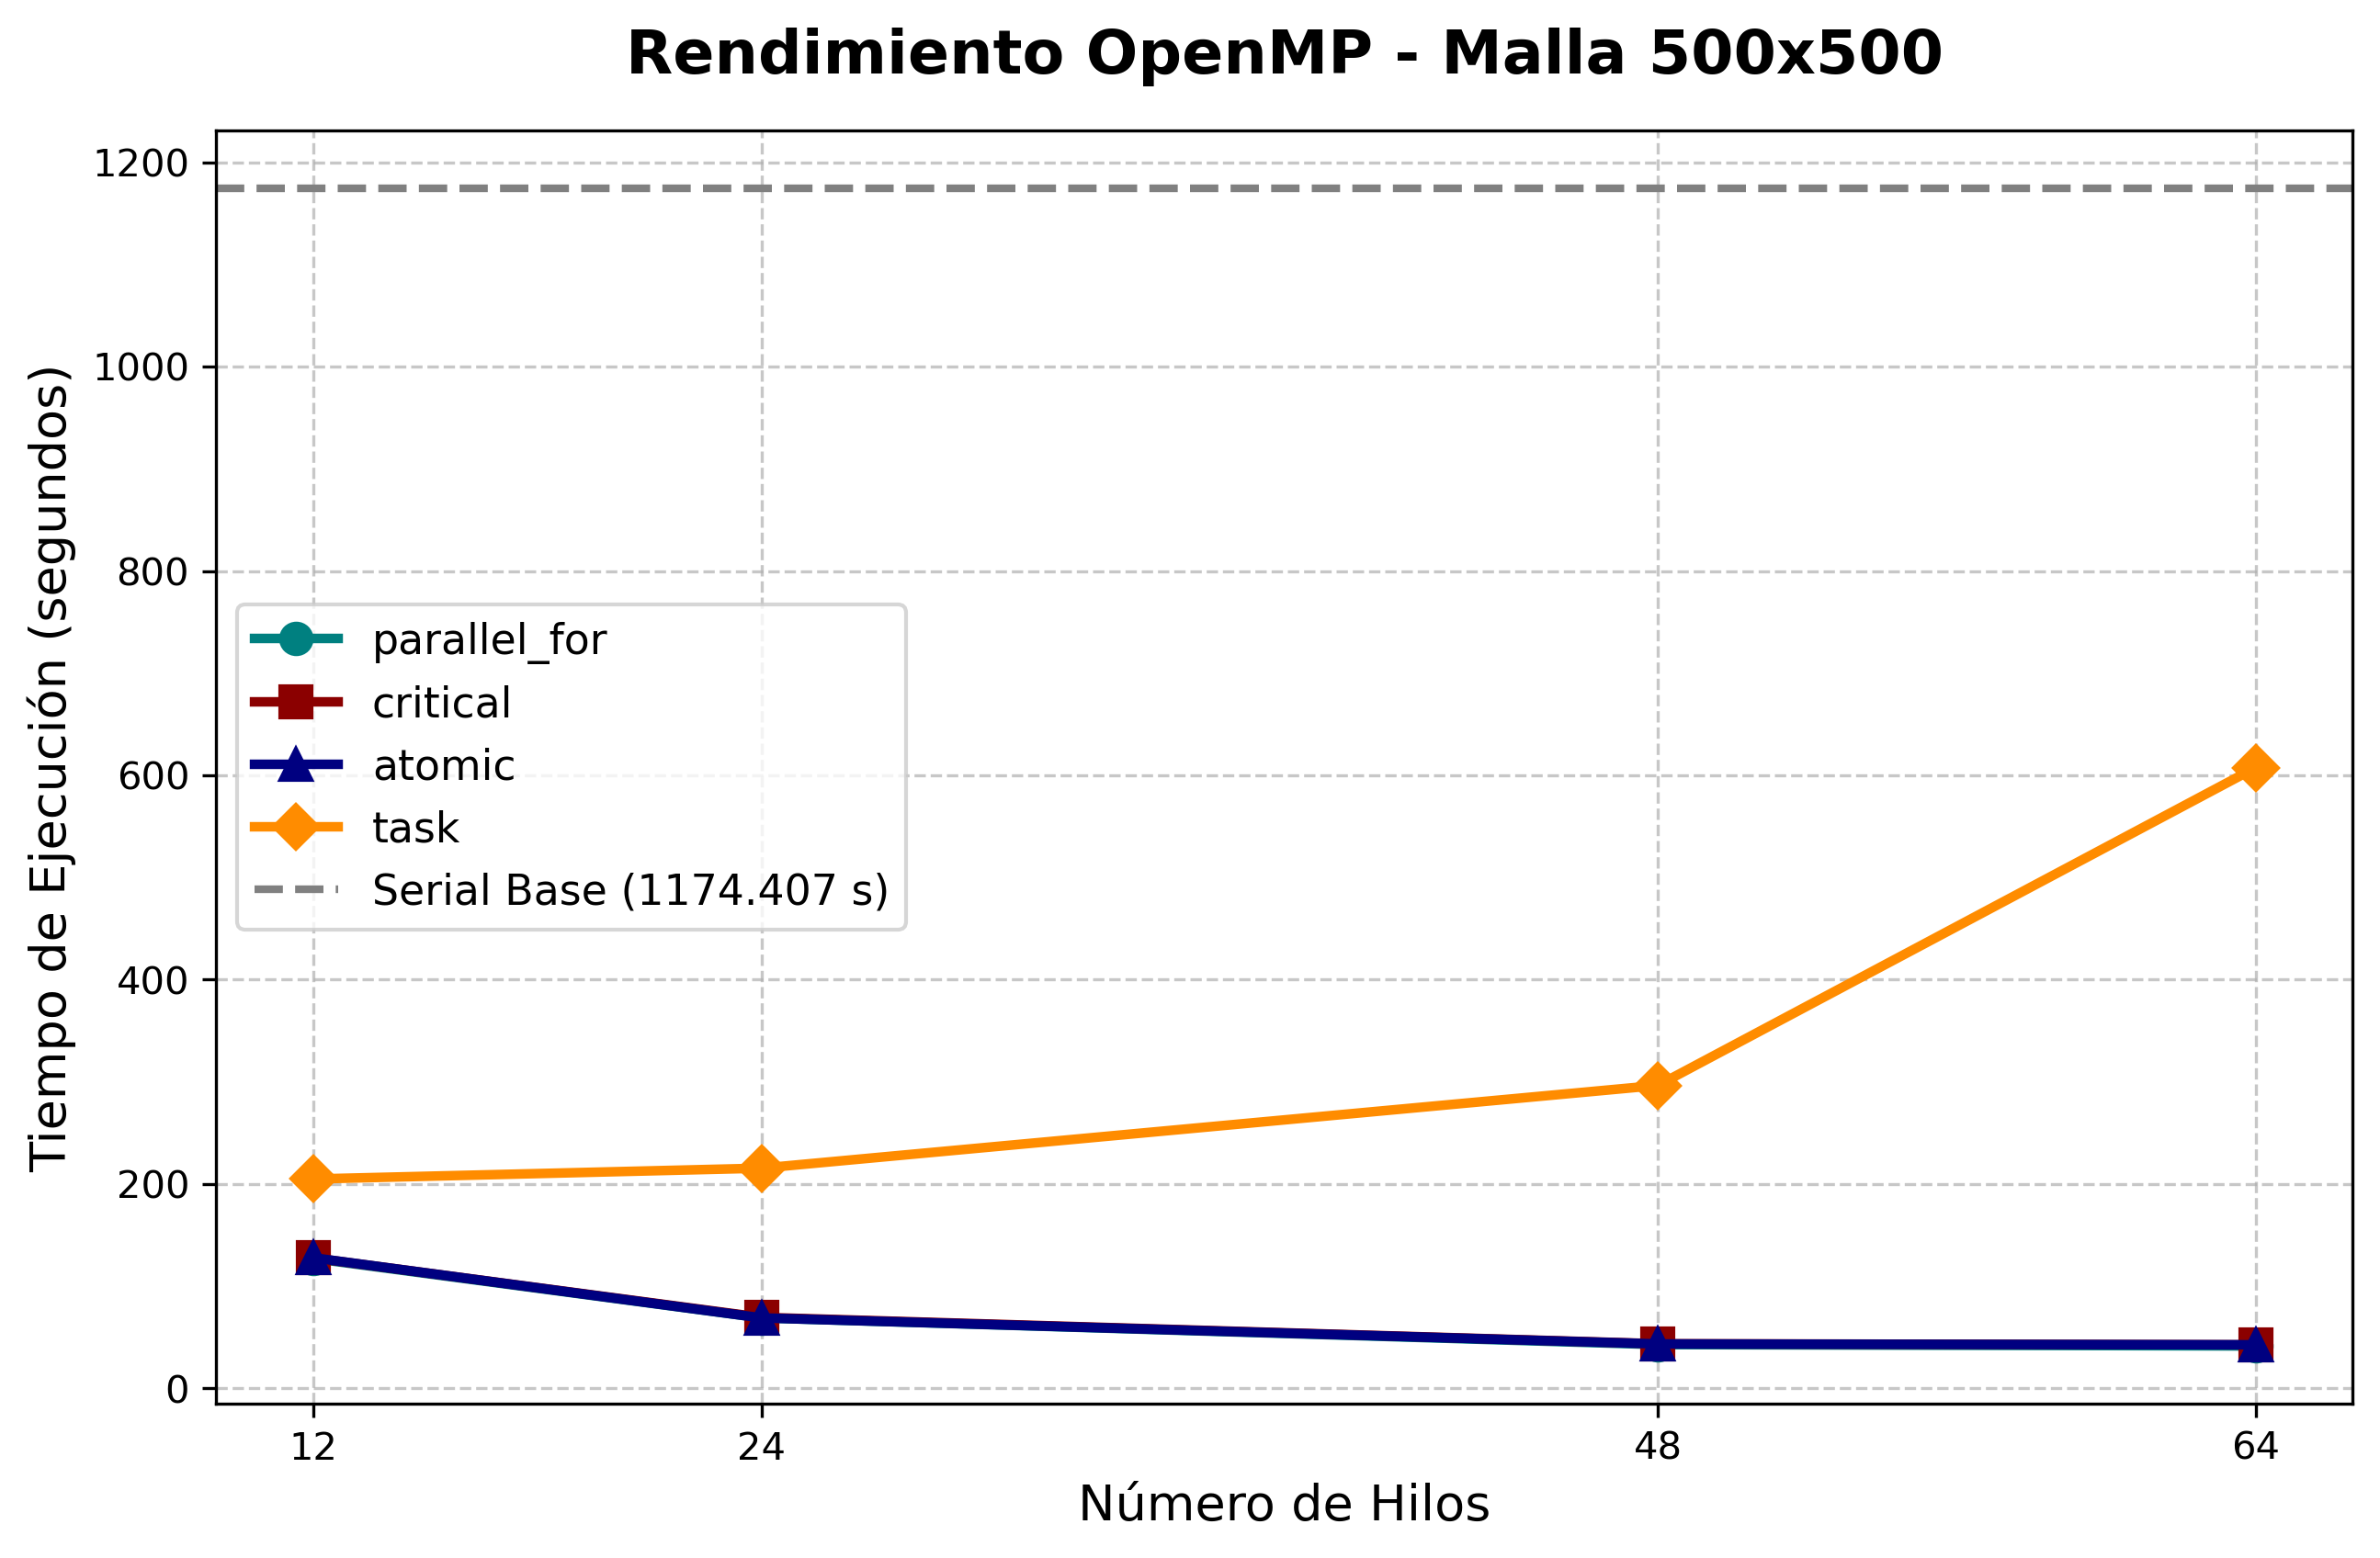
\includegraphics[width=0.8\textwidth]{imag/Rendimiento_Tiempos_N500.png}
    \caption{Tiempos de ejecución para la malla masiva de $500 \times 500$. La convergencia en un solo núcleo requiere 1174 s (casi 20 minutos). Las directivas de bucle y variables compartidas logran escalar eficientemente hasta los 64 hilos, reduciendo el cálculo a $\sim 41.5$ s.}
\end{figure}

\begin{figure}[H]
    \centering
    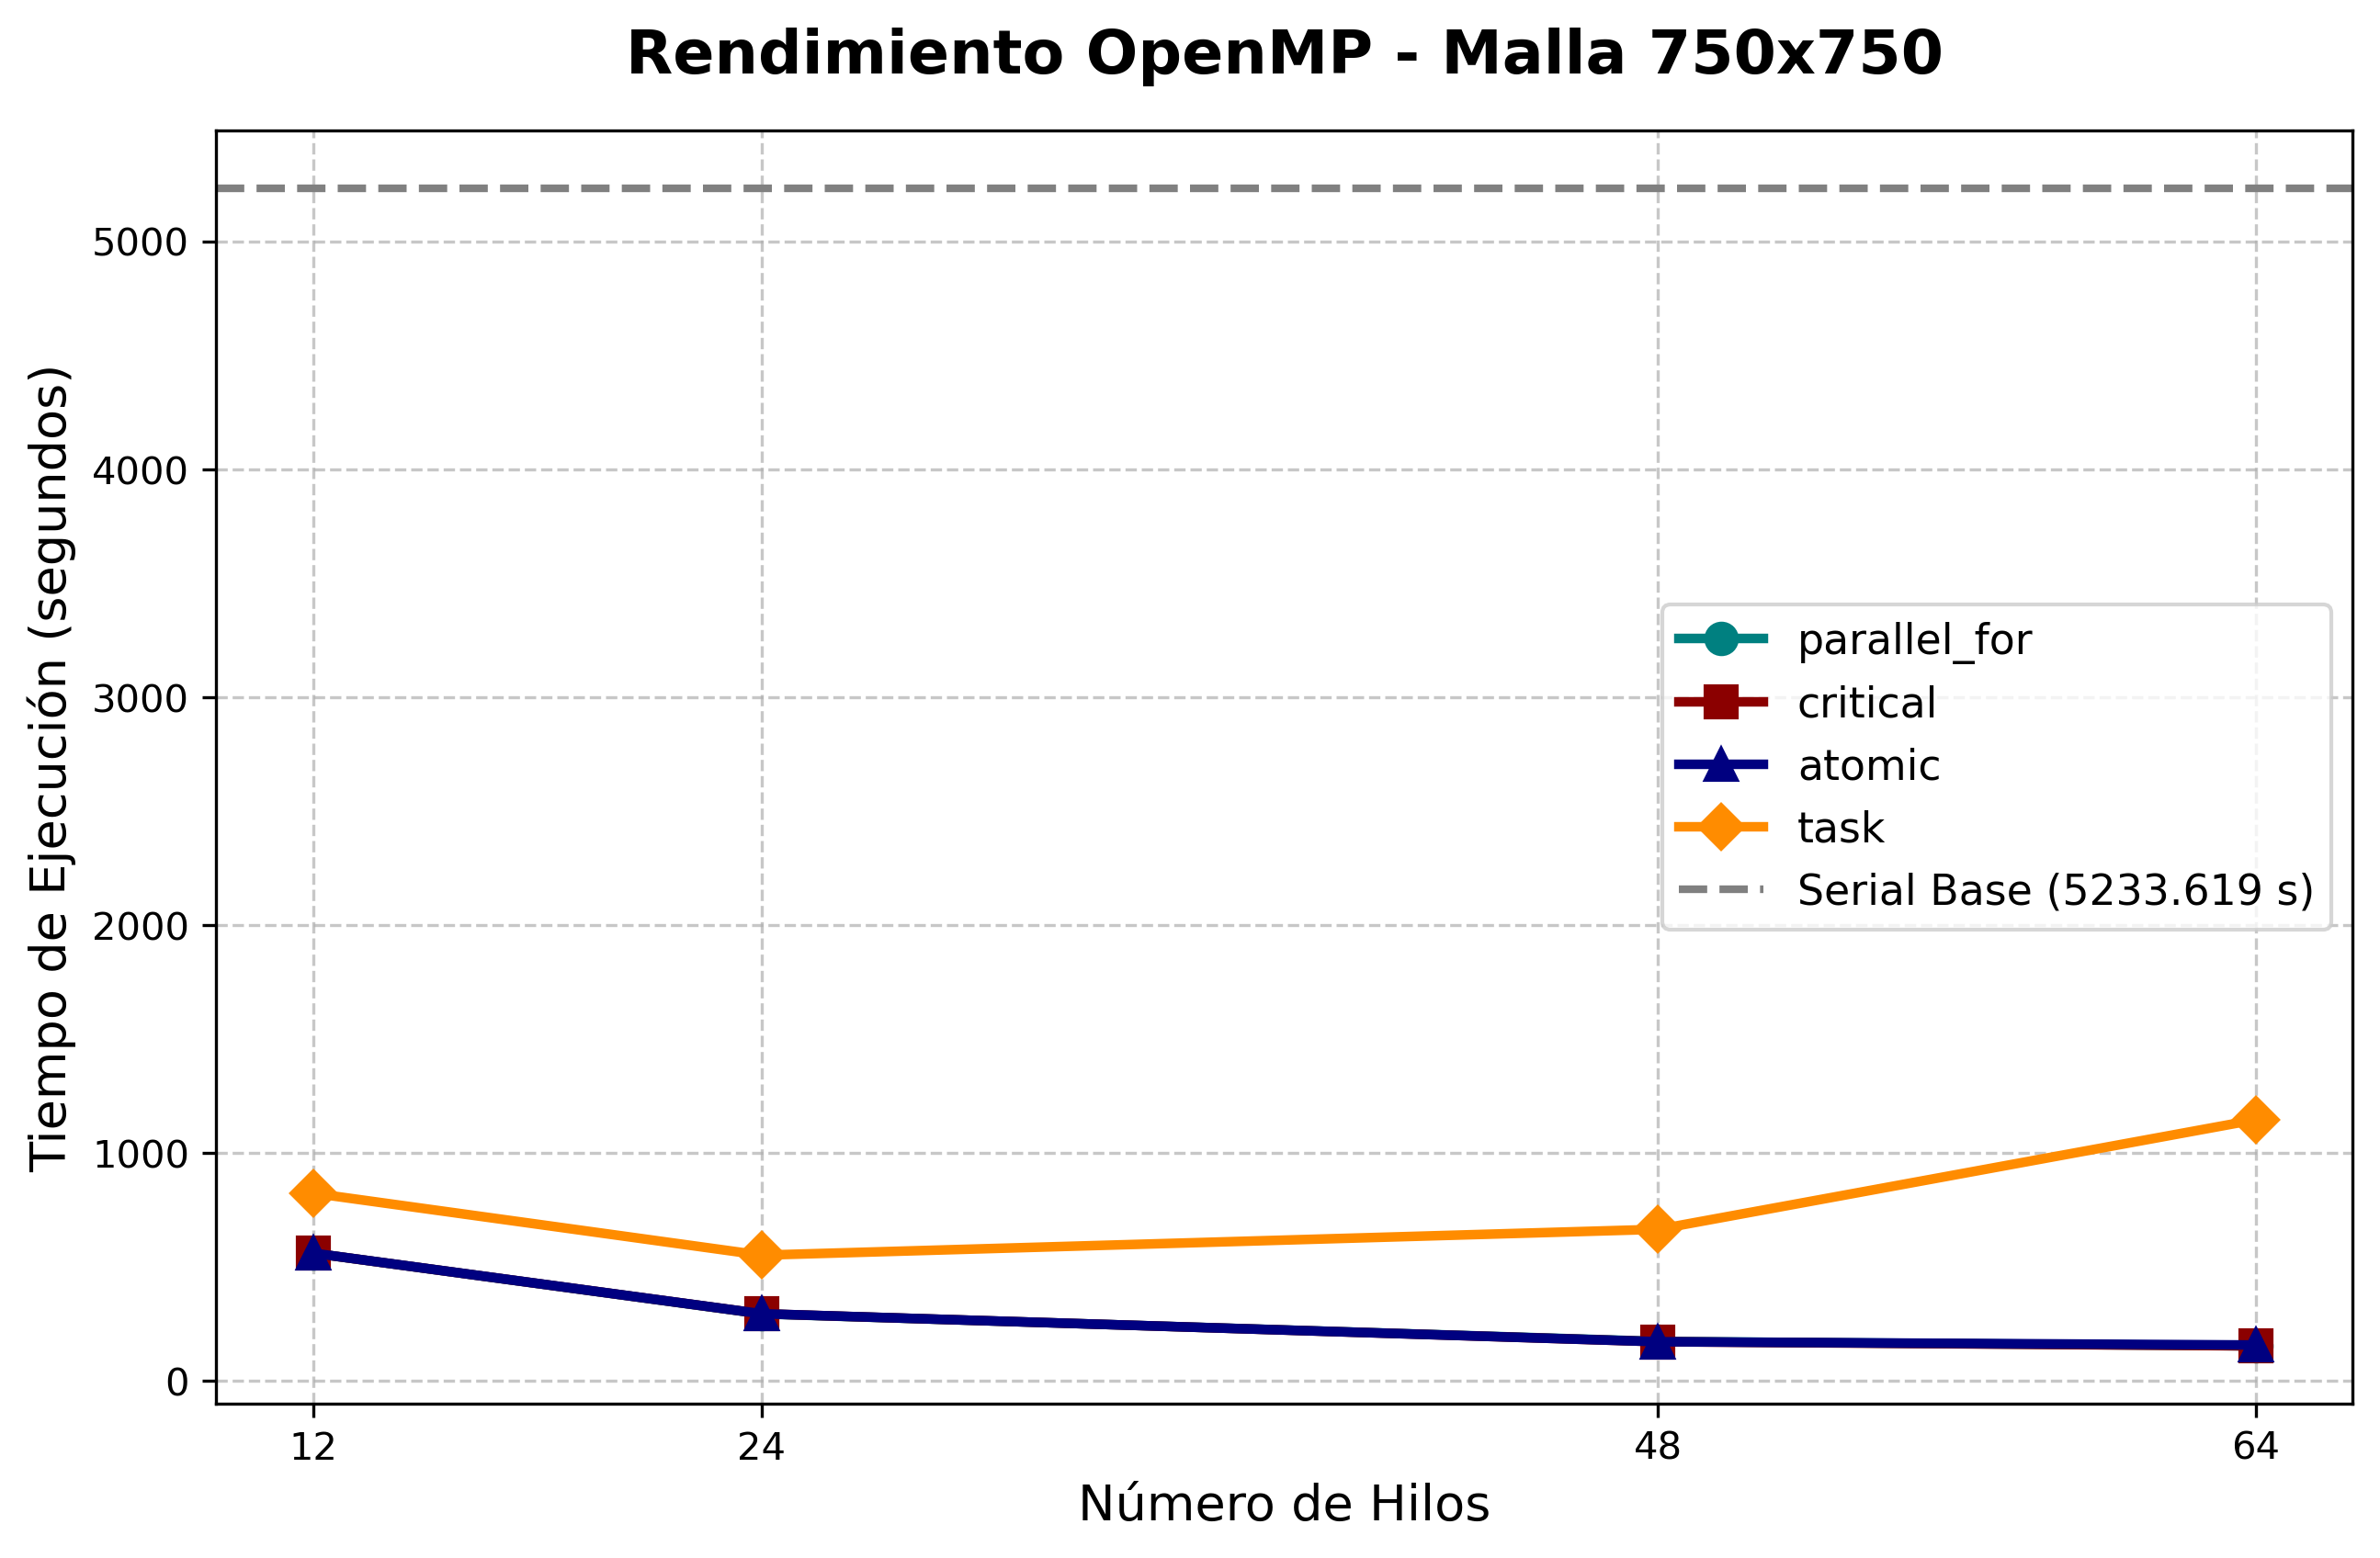
\includegraphics[width=0.8\textwidth]{imag/Rendimiento_Tiempos_N750.png}
    \caption{Tiempos de ejecución para la malla de $750 \times 750$. Bajo esta carga extrema, la ejecución serial sobrepasa los 5233 s. El paralelismo demuestra una escalabilidad sobresaliente y continua, consolidando su menor tiempo (154.2 s) con la capacidad máxima de 64 hilos.}
\end{figure}







\subsection{Análisis de Convergencia: Relajación Asíncrona en Memoria Compartida}

Para validar la exactitud de las soluciones numéricas y comprender la dinámica interna de OpenMP, se instrumentaron las implementaciones \texttt{poisson\_critical} y \texttt{poisson\_atomic}. El objetivo fue contabilizar el número exacto de iteraciones que requirió el bucle principal \texttt{while} para satisfacer la tolerancia estricta ($\Delta < 10^{-6}$).

El análisis de los registros de ejecución (\textit{logs}) del clúster revela un comportamiento no determinista fundamental en la computación paralela, evidenciado en la siguiente tabla de convergencia para diferentes tamaños de malla ($N$):

\begin{table}[H]
    \centering
    \begin{tabular}{|c|c|c|c|c|}
        \hline
        \textbf{Tamaño de Malla} & \textbf{Hilos} & \textbf{Iteraciones (\texttt{poisson\_critical})} & \textbf{Iteraciones (\texttt{poisson\_atomic})} \\ \hline
        \multirow{4}{*}{$N = 100$} 
        & 12 & 10,386 & 10,386 \\ \cline{2-4}
        & 24 & 10,385 & 10,385 \\ \cline{2-4}
        & 48 & 10,405 & 10,397 \\ \cline{2-4}
        & 64 & 10,494 & 10,519 \\ \hline
        \multirow{4}{*}{$N = 250$} 
        & 12 & 53,259 & 53,259 \\ \cline{2-4}
        & 24 & 53,258 & 53,258 \\ \cline{2-4}
        & 48 & 53,256 & 53,256 \\ \cline{2-4}
        & 64 & 53,254 & 53,254 \\ \hline
        \multirow{4}{*}{$N = 500$} 
        & 12 & 177,846 & 177,846 \\ \cline{2-4}
        & 24 & 177,845 & 177,845 \\ \cline{2-4}
        & 48 & 177,843 & 177,843 \\ \cline{2-4}
        & 64 & 177,841 & 177,841 \\ \hline
        \multirow{4}{*}{$N = 750$} 
        & 12 & 353,882 & 353,882 \\ \cline{2-4}
        & 24 & 353,881 & 353,881 \\ \cline{2-4}
        & 48 & 353,879 & 353,879 \\ \cline{2-4}
        & 64 & 353,877 & 353,877 \\ \hline
    \end{tabular}
    \caption{Número total de iteraciones necesarias para la convergencia variando el tamaño de la malla ($N$) y el número de hilos, comparando los dos métodos de sincronización explícita.}
    \label{tab:convergencia_iteraciones}
\end{table}

De estos datos empíricos se extraen dos conclusiones arquitectónicas críticas sobre las implementaciones desarrolladas:

\subsubsection{1. Carga Computacional Ligada a la Geometría}
La tabla ilustra que el esfuerzo iterativo depende de manera superlineal del tamaño de la malla geométrica ($N$). Pasar de una malla de $100 \times 100$ a una de $750 \times 750$ (un aumento de factor $7.5$ por lado) dispara la cantidad de barridos necesarios de $\sim 10,386$ a $\sim 353,882$ iteraciones (un factor cercano a $34\times$). Este crecimiento masivo en el número de iteraciones requeridas explica el colapso del rendimiento secuencial (\texttt{poisson\_serial}) en las mallas de 500 y 750, haciendo imperativa la división de la carga de trabajo entre múltiples núcleos.

\subsubsection{2. Relajación Asíncrona (Caótica) y Variación Numérica}
Al observar los datos dentro de una misma malla (por ejemplo, $N=500$ o $N=750$), se nota que \textbf{la cantidad de iteraciones no es una constante matemática fija}, sino que \textbf{disminuye levemente} al incrementar el número de hilos. Además, en condiciones de contención extrema (como en $N=100$ con 48 y 64 hilos), \texttt{critical} y \texttt{atomic} arrojan números de iteraciones notablemente distintos (ej. 10,494 vs. 10,519).

Esto ocurre porque las implementaciones en C++ carecen de un doble búfer estricto (como exigiría un método de Jacobi puro). Todos los hilos leen y sobrescriben la misma matriz \texttt{T} simultáneamente. Cuando el planificador de OpenMP altera la cantidad de hilos, modifica las "fronteras" de memoria donde los núcleos vecinos intercambian datos. 
Dependiendo de la latencia de la caché y de qué hilo ejecute su ciclo for más rápido, una celda puede calcular su promedio utilizando datos "viejos" (iteración $k$) o datos "recién actualizados" por otro hilo vecino (iteración $k+1$). Esta asincronía en la propagación de la información acelera o retrasa sutilmente el flujo global del error, alterando el conteo final de iteraciones de forma no determinista, aunque convergiendo siempre al mismo resultado físico válido.





\subsection{Desarrollo y Reflexiones del Taller}

A continuación, se da respuesta a las interrogantes planteadas en la guía del proyecto, fundamentadas en el comportamiento analizado durante la ejecución en el clúster computacional.

\subsubsection*{Actividad 1: Uso de \texttt{\#pragma omp parallel for} y \texttt{reduction}}
\begin{itemize}
    \item \textbf{¿Por qué es necesaria la cláusula \texttt{reduction}?} \\
    En el algoritmo de diferencias finitas, la variable \texttt{delta} almacena el error máximo de toda la malla para determinar la condición de parada del bucle \texttt{while}. Si múltiples hilos intentan sobrescribir esta variable simultáneamente utilizando \texttt{std::max}, se produce una condición de carrera (\textit{race condition}), corrompiendo el resultado. La cláusula \texttt{reduction(max:delta)} crea una copia privada de la variable para cada hilo y, al finalizar la región paralela, combina estos valores locales de forma segura utilizando el operador máximo.
    \item \textbf{¿Hubo mejora de rendimiento?} \\
    El rendimiento mejoró significativamente, pero su éxito dependió enteramente del tamaño del problema. Para mallas masivas ($750 \times 750$), el tiempo de cálculo se redujo en órdenes de magnitud. Sin embargo, para mallas pequeñas ($100 \times 100$), el rendimiento llegó a empeorar o estancarse al usar demasiados hilos debido al \textit{overhead} administrativo de instanciar y sincronizar.
    \item \textbf{¿Hubo diferencia en el número de iteraciones?} \\
    Sí, aunque de forma muy leve (variaciones de 1 a 5 iteraciones en cientos de miles). Al no implementar un esquema de doble búfer estricto, los hilos leen y escriben sobre la matriz simultáneamente. Esto genera \textbf{relajación asíncrona}: la variación en la velocidad de los hilos cambia ligeramente el flujo de la información, alterando la cantidad final de iteraciones dependiendo de la cantidad de hilos utilizados.
\end{itemize}

\subsubsection*{Actividad 2: Cláusula \texttt{collapse(2)}}
\begin{itemize}
    \item \textbf{¿Qué hace \texttt{collapse(2)}?} \\
    Esta directiva fusiona los dos bucles \texttt{for} anidados (iteradores $i$ y $j$) en un único espacio de iteración lineal de tamaño $M \times N$. Esto le permite a OpenMP distribuir una cantidad mucho mayor de tareas individuales entre los hilos, mejorando drásticamente el balanceo de carga (\textit{load balancing}).
    \item \textbf{¿Es siempre recomendable su uso?} \\
    No siempre. Solo es recomendable si los bucles anidados son "perfectamente anidados" (sin código intermedio entre el primer \texttt{for} y el segundo) y si el bucle exterior no tiene suficientes iteraciones para mantener a todos los hilos ocupados de forma óptima.
\end{itemize}

\subsubsection*{Actividad 3: Paralelización con \texttt{sections}}
\begin{itemize}
    \item \textbf{¿Vale la pena paralelizar funciones tan rápidas como la inicialización?} \\
    En el contexto de la ecuación de Poisson iterativa, \textbf{no vale la pena}. La inicialización y el cálculo de la matriz fuente se ejecutan \textbf{una sola vez} al inicio del programa. El costo (\textit{overhead}) computacional de crear un equipo de hilos y gestionar regiones \texttt{sections} supera las fracciones de milisegundo que tardan estas funciones en ejecutarse secuencialmente. El esfuerzo de paralelización debe enfocarse siempre en los cuellos de botella reales.
\end{itemize}

\subsubsection*{Actividad 4: Políticas de Planificación (\texttt{schedule})}
\begin{itemize}
    \item \textbf{Comparativa \texttt{static} vs \texttt{dynamic}:} \\
    Para este proyecto específico de diferencias finitas en una grilla uniforme, \texttt{schedule(static)} resulta ser la estrategia óptima. Al ser un dominio rectangular, el costo computacional de actualizar cada celda es exactamente el mismo. La política estática asigna los bloques de trabajo en tiempo de inicio, minimizando el \textit{overhead}. La política \texttt{dynamic} añade una sobrecarga innecesaria al pausar la ejecución para reasignar bloques de trabajo a los hilos que van terminando.
\end{itemize}

\subsubsection*{Conclusiones Generales}
\begin{enumerate}
    \item \textbf{¿Cuál fue la versión más rápida?} \\
    La versión \texttt{poisson\_parallel\_for} integrando la cláusula \texttt{collapse(2)}. Logró reducciones de tiempo contundentes, alcanzando \textit{speedups} superiores a $\sim$33x en la malla de $750 \times 750$.
    \item \textbf{¿Qué directiva es más fácil de usar?} \\
    La directiva \texttt{\#pragma omp parallel for}. Basta con anteponerla a un bucle \texttt{for} estándar garantizando la independencia de las variables, ocultando toda la complejidad de la instanciación de hilos y barreras de sincronización implícitas.
    \item \textbf{¿Hubo directivas que empeoraron el rendimiento? ¿Por qué?} \\
    Sí, la directiva \texttt{task} en general, y el exceso de hilos (64) en matrices pequeñas ($N=100$). El rendimiento se desplomó porque la contención en memoria y el \textit{overhead} introducido por OpenMP para administrar los hilos y las colas de tareas superó por completo el tiempo real de cómputo matemático.
\end{enumerate}

\subsubsection*{Actividad 5: \texttt{nowait}, \texttt{barrier}, \texttt{single}, \texttt{critical} (Control de sincronización)}
\begin{itemize}
    \item \textbf{Tiempo con \texttt{nowait} y cambios respecto al uso por defecto:} \\
    Al añadir \texttt{nowait}, se elimina la barrera de sincronización implícita al final del bucle \texttt{for}. Si bien esto reduce levemente el tiempo al evitar que los hilos rápidos esperen a los lentos, en la ecuación de Poisson genera un cambio desastroso si se usa mal: los hilos \textbf{deben} sincronizarse (\textit{barrier}) antes de pasar a la iteración $k+1$ o antes de evaluar la tolerancia del error. Si un hilo avanza y sobrescribe la matriz mientras otros siguen leyendo, la simulación física se corrompe por completo.
    \item \textbf{¿Dónde colocaste la directiva \texttt{single} y por qué?} \\
    La directiva \texttt{single} se ubicó estratégicamente al inicio de la región paralela del bucle \texttt{while} (por ejemplo, en la implementación con \texttt{task}) para inicializar variables bandera o imprimir el inicio del cálculo. Se utiliza ahí porque asegura que \textbf{un solo hilo} ejecute esa instrucción administrativa mientras los demás lo ignoran, evitando impresiones repetidas en la consola o el reinicio de variables por parte de múltiples hilos.
    \item \textbf{¿\texttt{critical} ralentizó la ejecución? ¿En qué contexto sería útil?} \\
    Sí, colocar un bloque \texttt{critical} detiene el flujo concurrente y genera un cuello de botella severo, ralentizando drásticamente la ejecución si se evalúa millones de veces. Sin embargo, es inmensamente útil y obligatorio en contextos donde varios hilos deben realizar operaciones no atómicas sobre recursos compartidos, como por ejemplo: comparar y actualizar el error máximo global (\texttt{std::max}), o proteger la escritura en los archivos de datos (\texttt{.dat}) para que el texto de diferentes hilos no se mezcle en el archivo de salida.
\end{itemize}

\subsubsection*{Actividad 6: Sincronización y Acceso Compartido (\texttt{critical} vs \texttt{atomic})}
En esta actividad se abordó el problema de las condiciones de carrera (\textit{Race Conditions}) al intentar que múltiples hilos contabilicen el número total de iteraciones sobre una misma variable compartida (\texttt{iterations}). Para proteger esta variable y garantizar que la suma sea exacta, se implementaron y compararon dos directivas de sincronización de OpenMP: \texttt{\#pragma omp critical} y \texttt{\#pragma omp atomic}.

A partir de los resultados empíricos obtenidos en el clúster y el análisis de la arquitectura de la API, se da respuesta a las interrogantes planteadas:

\textbf{¿Qué diferencias observas en el rendimiento entre usar \texttt{critical} y \texttt{atomic}?} \\
Aunque en mallas pequeñas el impacto queda enmascarado por la rapidez del cálculo, a nivel de arquitectura la diferencia de rendimiento radica en cómo gestionan el bloqueo bajo cargas de alta contención (por ejemplo, con 48 o 64 hilos):
\begin{itemize}
    \item \textbf{\texttt{critical}:} Genera un \textbf{bloqueo a nivel de software} (mutex). Obliga al sistema operativo a intervenir, poniendo en estado de espera (suspensión) a los hilos que intentan acceder al bloque mientras otro lo está ocupando. Esto genera un alto \textit{overhead} administrativo, ralentizando la ejecución si miles de iteraciones compiten por el candado.
    \item \textbf{\texttt{atomic}:} Genera un \textbf{bloqueo a nivel de hardware}. Utiliza instrucciones directas del procesador (como \textit{Compare-And-Swap}) para asegurar que la actualización en la dirección de memoria de la variable se realice en un solo ciclo de reloj indivisible. Es inmensamente más rápido y eficiente, ya que evita que los hilos entren en estado de suspensión, reduciendo drásticamente el cuello de botella.
\end{itemize}

\textbf{¿En qué casos sería preferible una sobre la otra?} \\
La elección entre ambas directivas depende estrictamente de la complejidad de la operación que se necesita proteger:
\begin{itemize}
    \item \textbf{Se prefiere \texttt{atomic}:} Cuando se requiere proteger operaciones matemáticas simples, rápidas y elementales sobre \textbf{una única variable} en memoria (por ejemplo: incrementos \texttt{++}, decrementos \texttt{--}, sumas \texttt{+=}, restas o multiplicaciones). Es la opción obligatoria para contadores y acumuladores globales debido a su nulo impacto en el rendimiento.
    \item \textbf{Se prefiere \texttt{critical}:} Cuando la sección de código a proteger es compleja y no puede ser traducida a una instrucción atómica de hardware. Es indispensable si se necesita ejecutar bloques enteros de código secuencial, evaluar sentencias condicionales (\texttt{if-else}), manipular múltiples variables simultáneamente, o escribir datos en la salida estándar (como el uso de \texttt{std::cout} o escritura en archivos \texttt{.dat} para evitar que el texto de los hilos se superponga).
\end{itemize}

\subsubsection*{Actividad 7: Exploración con Tareas (\texttt{task})}
\begin{itemize}
    \item \textbf{¿Cómo se compara el rendimiento usando \texttt{task} con respecto a \texttt{parallel for}?} \\
    La estrategia basada en \texttt{task} arrojó consistentemente los \textbf{peores tiempos} en todo el benchmark. En el caso masivo ($750 \times 750$ con 64 hilos), el método por tareas requirió más de 1146 segundos, en marcado contraste con los 154 segundos del \texttt{parallel for collapse}.
    \item \textbf{¿Qué ventajas y desventajas tiene este enfoque?} \\
    \textit{Ventajas:} El enfoque de tareas es extraordinariamente potente para estructuras de datos irregulares o dinámicas (como listas enlazadas), algoritmos recursivos (como Fibonacci o Merge Sort) y bucles \texttt{while} sin límites definidos. \\
    \textit{Desventajas:} Para arreglos densos y predecibles (como las matrices de diferencias finitas), el costo administrativo de instanciar tareas en OpenMP, agregarlas a una cola en memoria compartida y esperar a que los hilos las reclamen, ahoga por completo al procesador y destruye la escalabilidad.
\end{itemize}
\end{document}



